% arara: pdflatex
% arara: biber
% arara: pdflatex
% arara: pdflatex
\documentclass[tufte-book,notoc,biblatex={citestyle=authoryear, autocite=footnote}]{tufte-thesis}

\usepackage{tikz}
\usetikzlibrary { graphs , automata , quotes , cd }

\usepackage{logic}
\RenewDocumentCommand \limp { } { \mathbin { \setminus } }
\RenewDocumentCommand \pmir { } { \mathbin { / } }

\usepackage{proof-dashed}
% \usepackage{mathpartir}
% \ExplSyntaxOn
%   \cs_set_eq:NN \__infer:nn \infer
%   \RenewDocumentCommand \infer { m m }
%     { \__infer:nn {#2} {#1} }
% \ExplSyntaxOff

\usepackage{singleton}

\usepackage{thesis-macros}

\usepackage{pbox}

\newcommand* \ie {\textit{i.e.}}
\newcommand* \alertnote [1]{\footnote{\color{red} #1}}

%%% Local Variables:
%%% mode: latex
%%% TeX-master: "thesis"
%%% End:


\usepackage{lipsum}

\title{Untitled thesis}
\author{Henry DeYoung}

\addbibresource{thesis.bib}

\begin{document}

\frontmatter

\maketitle
\tableofcontents
\listoffigures
\listoftables

\mainmatter

\chapter{Introduction}\label{ch:introduction}

\fixnote{Simple example throughout introduction?}

\begin{itemize}
\item
  Concurrency is notoriously difficult to get right.
  \begin{itemize}
  \item For functional programming, Curry--Howard application of proof theory is the gold standard.
  \item Since Girard, efforts to explain concurrency using proof theory.
  \end{itemize}

\item 
  Two proof-theoretic ways to characterize concurrency:
  \begin{itemize}
  \item proof construction as concurrency
  \item proof reduction as concurrency
  \end{itemize}
  Each has its own strengths and weaknesses.
  Relatively little (none?) study of the relationship between these characterizations.

\item
  Proof reduction $\cong$ session-typed processes (SILL).
  \begin{itemize}
  \item Strengths: behavioral types; preservation and progress; process implementation;
                   logical extensions suggest new features
  \item Weaknesses: very local description (cf.\ local and global session types);
                    synchronous communication
  \end{itemize}
  Good for implementation.

\item
  Proof construction $\cong$ process-as-formula (Miller et al.),
                             multiset rewriting (Cervesato and Scedrov).
  \begin{itemize}
  \item Strengths: more global description (though slightly lower level than global types?);
                   \emph{a}synchronous communication;
  \item Weaknesses: untyped; can deadlock; less obviously extensible;
                    specification, but not implementation
  \end{itemize}
  Good for specification.

\item
  Where do the proof reduction and proof construction characterizations intersect?
  \begin{itemize}
  \item Intersection will have strengths of both, with weaknesses of neither.
  \item On the intersection, a proof-construction specification can be \enquote{projected} to a proof-reduction implementation.
  \end{itemize}

\item
  To focus our attention on the essential differences between proof reduction and proof construction, we limit our investigation to chain topologies, not the more general tree topologies of SILL.
  \begin{itemize}
  \item Chain topologies let us treat channels namelessly, which turns out to lift a large notational burden.
  \item In both the proof reduction and proof construction chacterizations, there are logical justifications for chain topologies.
  \item We conjecture that our results can be straightforwardly generalized to tree topologies, with a large notational overhead, but no conceptual difficulties.
  \end{itemize}

\item
  Outline of chapters and discussion of contributions

\item
  Abstract rewriting, specifically string rewriting, as a framework for specifying the dynamics of concurrent systems.
  \begin{itemize}
  \item Systems with components arranged in a linear topology with a monoidal structure 
  \item Special case of multiset rewriting (Cervesato and Scedrov), so not a contribution of this work
  \item Introduce running examples for the first time: NFAs and binary counters.
    (A review of finite automata can be found in \cref{ch:finite-automata}.)
  \end{itemize}

\item
  Ordered rewriting generalizes string rewriting to a richer set of \enquote{connectives} -- free residuated lattice, not just a free monoid
  \begin{itemize}
  \item Based on the ordered sequent calculus of \cref{ch:ordered-logic}
  \item Ordered rewriting justified by refactoring the sequent calculus left rules to eliminate boilerplate.
    \begin{itemize}
    \item Rewriting is obtained as a fragment of the refactored calculus
    \item This derivation appears to be an auxiliary contribution of this work
    \end{itemize}
  \item Roughly a special case of (Cervesato and Scedrov)
  \item \emph{Focused} ordered rewriting to control the atomicity of individual rewriting steps
  \end{itemize}

\item 
  Both string rewriting and (focused) ordered rewriting are global, state transformation systems.
  \begin{itemize}
  \item Our goal is to identify a fragment (intersection) that acts like a process calculus -- a local, formula-as-process interpretation.
    \begin{itemize}
    \item Propositions as process expressions, contexts as runtime process configurations, atoms as messages 
    \item Surprisingly few changes needed: atom directions and syntactic restriction placed on implications
    \item Not really a contribution?  (Miller et al.)
    \end{itemize}
  \item coinductively defined propositions, not replication, for unbounded rewriting 
  \item Major contribution of this chapter: proceedure for choreographing string rewriting specifications into formula-as-process ordered rewriting
    \begin{itemize}
    \item Role assignment to each symbol -- message or process
    \item Not all role assignments lead to sensible choreographies
    \item String rewriting axioms used as an evaluation\fixnote{word choice?} -- specification and choreography must be bisimilar.
      [First appearance of a bisimiarity.  States' structures are observable]
    \item Informal description, then formal description 
    \end{itemize}
  \item Choreographies for binary counters and NFAs 
    \begin{itemize}
    \item End-to-end adequacy of choreography as a composition of specification's adequacy with bisimilarity of choreography and specification
    \item NFA example leads to a desire for an equivalence coarser than equality 
    \end{itemize}
  \end{itemize}

\item A notion of bisimilarity for ordered rewriting
  \begin{itemize}
  \item observatinal equivalence: prepositions/processes are opaque; atoms/messages are observable 
    \begin{itemize}
    \item very much dependent on formula-as-process interpretation
    \end{itemize}
  \item Contribution?  Related to (Deng et al.) but our formulation is different
  \item Labeled bisimilarity as a sound (and complete!) proof technique for rewriting bisimilarity
  \item Examples of bisimilarity: NFA encoding preserves bisimilarity; bisimilarity of binary counters coincides with equal denotations 
  \end{itemize}

\item That closes proof construction.  Now for proof reduction.

\item Singleton logic
  \begin{itemize}
  \item Independently identified by (Fortier and Santocanale)
  \end{itemize}
\end{itemize}

 






























































\subsection{}

\begin{itemize}
\item Computation as deduction: clear, expressive, and provably correct programs
  \begin{itemize}
  \item Examples of sucess stories
  \item Can it be applied to concurrency?
  \end{itemize}
\item Proof constuction and proof reduction views of con currency
  \begin{itemize}
  \item Proof construction: good for specifications 
  \item Proof reduction: good for implementions 
  \end{itemize}
\item Thesis statement: Session types bridge these two views
\item Ordered logic as a proving ground 
  \begin{itemize}
  \item Ordered rewriting for proof construction
  \item Singleton logic (purely additive fragment of ordered logic) for proof reduction
  \end{itemize}
\item Ordered rewriting (chapter 4) for specifications
  \begin{itemize}
  \item DFAs and NFAs 
  \item Binary counters
  \end{itemize}
\item Refinement of ordered rewriting for choreographies (chapter 5)
  \begin{itemize}
  \item Recursive definitions as processes; atoms as messages 
  \item Untyped (mostly, except for directions)
  \item Rewriting bisimilarity for observational equivalence
    \begin{itemize}
    \item Examples
    \end{itemize}
  \end{itemize}
\item Singleton logic and its semi-axiomatic calculus (chapter 6)
\item 
\end{itemize}


Concurrent systems are notoriously difficult to get right.

Beginning with Curry's observation that Hilbert [...] corresponds to a form of computation based on combinatory reduction\autocite{??}, and continuing with Howard's discovery of an isomorphism between [Gentzen's] intuitionistic natural deduction and Church's simply-typed $\lambda$-calculus, computation-as-deduction has been the gold standard for clear, expressive, and provably correct programs.

Computation-as-deduction can be divided into two classes: proof-search-as-computation and proof-reduction-as-computation.
The former provides a logically grounded basis for the backward- and forward-chaining logic programming paradigms, whereas the latter is the foundation for the functional programming paradigm.

Logically grounded concurrent computation 

More recently, a proof-reduction description of concurrency has been discovered by \textcite{??} with \textcite{??}.
In this isomorphism, linear propositions correspond to session types; sequent proofs, to session-typed processes; and cut reduction, to synchronous message-passing communication.

This thesis seeks to bring these two apparently divergent views of concurrency together.
Is there a class of specifications for which well-typed implementations can automatically be extracted?

Thesis statement: Session types form the bridge. 


\section{Proposal introduction}

With the increasingly complex, distributed nature of today's software systems, concurrency is ubiquitous.
Concurrency facilitates distributed computation by structuring systems as nondeterministic compositions of simpler subsystems.
But, concomitant with nondeterminism, concurrent systems are notoriously tricky to get right:
subtle races and deadlocks can occur even in the most rigorously tested of systems.

At the same time, decades of research into connections between proof theory and programming languages have firmly established the principle of \vocab{computation as deduction} as the gold standard [framework] for clear, expressive, and provably correct programs.
Most generally, intuitionistic logic is the bedrock for both the typed functional\autocite{Martin-Lof:LMPS80} and logic programming\autocites{Miller+:PAL91}{Andreoli:JLC92}\fixnote{check refs?} paradigms.
In more specific [...]
Examples abound: lax logic for effectful computation\autocite{Benton:JFP98}, temporal logic for functional reactive programming\autocite{Jeffrey:PLPV12}, and linear logic for graph-based algorithms\autocite{Cruz+:ICLP14}, to name just a few.

Can a computation-as-deduction approach make it similarly easier to clearly and concisely specify, as well as correctly implement, concurrent programs?

\subsection{}

The principle of computation as deduction comes in two flavors: \vocab{proof construction as computation} and \vocab{proof reduction as computation}.
Under a proof-construction-as-computation view, the search for a proof, according to a fixed strategy, forms the basis of computation; it is the foundation for logic programming\autocites{Miller+:PAL91}{Andreoli:JLC92}.
The proof-reduction-as-computation view, on the other hand, revolves around a correspondence, known as the Curry--Howard Isomorphism\autocite{Curry:??}{Howard:??}, between propositions and types, proofs and programs, and proof simplification, or reduction, and program evaluation;
it is the foundation for typed functional programming\autocite{Martin-Lof:LMPS80}.

Both the proof-construction and proof-reduction approaches have been successfully applied to concurrent programming, originally stemming from \citeauthor{Girard:TCS87}'s suggestion of connections between linear logic and concurrency\autocite{Girard:TCS87}.
In the proof-construction vein, \acroifusedTF{CLF}{\ac{CLF}\autocite{Watkins+:CMU02}}{the \acf{CLF}\autocite{Watkins+:CMU02}} treats the permutability of inference rules as the source of concurrency.
\Ac{CLF} has been used to specify a variety of concurrent systems, ranging from the $\pi$-calculus to security protocols and even emergent story narratives\autocites{Cervesato+Scedrov:IC09}{Martens+:LPNMR13}.\fixnote{check refs}
Although these same concurrent systems can be simulated according to their \ac{CLF} specifications by the Lollimon\autocite{Lopez+:PPDP05} and Celf\autocite{Schack-Nielsen:ITU11} logic programming engines, the programs ultimately remain specifications, not actual \emph{decentralized} implementations.

Taking the other, proof-reduction tack, \textcite{Abramsky:TCS93}, \textcite{Bellin+Scott:TCS94}, and later \textcite{Caires+Pfenning:CONCUR10} with Toninho\autocites{Caires+:TLDI12}{Caires+:MSCS13} have given correspondences between sequent calculus proofs or proof nets in linear logic and processes; between cut elimination and concurrent process execution.
Moreover, in \citeauthor{Caires+:MSCS13}'s work, the correspondence is a true Curry--Howard isomorphism in that intuitionistic linear propositions are also types -- \vocab{session types}\autocite{Honda:CONCUR93} that describe the interaction protocol to which a process adheres.
Unlike proof construction, the proof-reduction approach yields actual decentralized implementations with independent threads of control\autocites{Toninho+:ESOP13}{Griffith+Pfenning:14}.

In spite of their common basis in linear logic, these proof-construction and proof-reduction approaches to concurrent computation appear at first glance to be strikingly disparate.
They have different dynamics; they offer different guarantees (session fidelity, behavioral type preservation, and deadlock freedom for the proof-reduction approach, but only non-behavioral type preservaton for the proof-construction approach); and, perhaps most importantly, they serve very different roles in programming practice.
Proof construction is better suited to system specification and reasoning, whereas proof reduction is better suited to implementation.

To reduce the possibiity of error when building an implementation from a specification, we would like to minimize the gap between the two.
Despite the apparent disparity between proof construction and proof reduction, is there a class of concurrent specifications from which decentralized concurrent implementations can be automatically extracted?
Stated differently, is there perhaps (some fragment of) a substructural logic in which the computational natures of proof construction and proof reduction coincide?

\subsection{}

The thesis is that, yes, we can indeed have our cake and eat it too:
\begin{quotation}
\normalsize\noindent
Thesis statement.
\itshape Session types form a bridge between distinct notions of concurrency in computational interpretations of ordered logic based on proof construction, on one hand, and proof reduction, on the other hand.
\end{quotation}

\Cref{part:preliminaries} reviews some necessary background information: definitions of nondeterministic and \aclp*{DFA}~\parencref{ch:automata}, and a sequent calculus presentation of ordered logic~\parencref{ch:ordered-logic}.
The reader should feel free to skim or skip these \lcnamecrefs{ch:automata} and return to them 

\newthought{\Cref{part:proof-construction} then delves} into a proof-construction approach to concurrency, beginning with a review of a framework for string rewriting~\parencref{ch:string-rewriting}.
Because disjoint segments of a string may be rewritten independently, string rewriting can be used to specify concurrent systems that have a linear topology.
The \lcnamecref{ch:string-rewriting} concludes with two extended examples of string rewriting specifications:
\aclp*{NFA}\footnote{And, as a special case, deterministic ones, too.}
and binary representations of natural numbers equipped with increment and decrement operations.
These will serve as running examples throughout this document.

Despite being concurrent, string rewriting specifications lack an immediate notion of local execution.
String rewriting presumes the existence of a central conductor that orchestrates the computation, rewriting the string globally.
Global rewriting, although reasonable for concurrent specifications, will not map well to locally executing process implementations that a proof-reduction approach to concurrency suggests -- the gap is simply too large.

Toward this end, \cref{ch:ordered-rewriting} presents an extension of the Lambek calculus\autocite{Lambek:??} in which string rewriting specifications may be refined into \vocab{choreographies}.
Inspired by the process-as-formula view of linear logic\autocites{Miller:??}{Cervesato+Scedrov:IC09}, choreographies exist at a slightly lower level of abstraction than string rewriting specifications in that they begin to introduce a message-passing character.
A choreography partitions a string rewriting specification's symbols into 

Having introduced a message-passing character and stronger notion of process identity, we can then ask when two processes are observationally equivalent.
\Cref{ch:ordered-bisimilarity} develops a notion of bisimilarity for ordered propositions, where the uninterpreted atoms are the only observables.

\subsection{Contributions}

The contributions of this thesis can be viewed from several perspectives.
\begin{itemize}
\item This work can be seen as a proof-theoretic [logical] reconstruction of multiparty session types~\autocite{Honda+:POPL08}.
In multiparty session types, binary session types are generalized to conversations among several parties.
Conversations in their entirety are specified using global session types.
Global types can be projected to binary session types for each pair of participants, which very nearly are implementations.
\item This work can be seen to further understanding of proof construction and proof reduction.
\item Gives types to logic programs.
Guarantees deadlock-freedom.
\end{itemize}
In addition to the practical benefit of 


The remainder of this document aims to establish this thesis as a plausible one.
To do so, we turn our attention from linear logic to (non-modal) intuitionistic ordered logic~\autocites{Lambek:AMM58}{Polakow+Pfenning:MFPS99}---a restriction of linear logic in which the context of hypotheses forms a list rather than a multiset or bag---and defend the thesis in this restricted setting.
The proposed thesis research is to relax the restrictions and expand the ideas in this document to intuitionistic linear logic.

Specifically, this document describes ... as depicted in \cref{fig:outline}.
First, \cref{?} reviews a string rewriting interpretation of proof construction in a [non-modal] fragment of intuitionistic ordered logic~\autocite{Simmons:CMU12}.
String rewriting specifications in this fragment are equipped with a natural notion of concurrency based on treating  as equivalent the different interleavings of independent rewriting steps.
[equivalence classes of proofs.]

Despite being concurrent, these string rewriting specifications lack an immediate notion of \emph{process} or \emph{process identity}.
Toward this end, \cref{?} introduces \vocab{choreographies}, a further restriction of string rewriting specifications obtained when [in which] atomic propositions are assigned roles as either process-like atoms or message-like atoms.
(Message-like atoms, such as  in \cref{fig:outline}, are indicated with an arrow decoration.)
A specification may admit several choreographies, but, as described in \cref{?}, a well-formed choreography must be (lock-step) equivalent with the specification.

Even with process-like atoms, choreographies remain string rewriting specifications, not actual distributed implementations of processes.
Nevertheless, choreographies are a stepping-stone to process implementations. 
In \cref{?}, we develop a session-typed process calculus from a Curry--Howard interpretation of a fragment of linear logic; 
\Cref{?} shows how choreographies can be compiled to 

Choreographies serve as a stepping stone to full-fledged process definitions.

%%% Local Variables:
%%% mode: latex
%%% TeX-master: "thesis"
%%% End:


\part{Preliminaries}

\chapter{Preliminaries: Automata}\label{ch:automata}

In this \lcnamecref{ch:automata}, we review the definitions of alphabets, words, languages, and automata that we will use in the running examples throughout this document.
% The classic text by \textcite{Hopcroft+Ullman:??} is a excellent reference.
Our definitions, though equivalent to the classical ones found in \textcite{Hopcroft+Ullman:??}'s text, differ slightly, having been tuned for the particular applications in this document.

\section{Alphabets, words, and languages}

An alphabet $\ialph$ is simply a set of symbols, $a \in \ialph$.
A finite word $w$ over the alphabet $\ialph$ is then a (possibly empty) finite sequence of symbols drawn from $\ialph$;
we denote the empty word by $\emp$.
The finite words form a free monoid under concatenation, with $\emp$ being the unit.
We denote by $\finwds{\ialph}$ the set of all finite words over $\ialph$.

It is also possible to construct infinite words.
An infinite word over the alphabet $\ialph$ is a countably infinite sequence of letters drawn from $\ialph$;
we denote the set of all infinite words over $\ialph$ by $\infinwds{\ialph}$.
We also use $\wds{\ialph}$ to denote the set of all words -- finite or infinite -- over the alphabet $\ialph$; that is, $\wds{\ialph} = \finwds{\ialph} \union \infinwds{\ialph}$.

A language is a set of words.
Depending on the context, it will be a subset of either $\wds{\ialph}$, $\infinwds{\ialph}$, or $\finwds{\ialph}$.

% It will sometimes be useful to work with an augmented alphabet.
% Given a symbol $c \notin \ialph$, we may form the augmented alphabet $\augalph{\ialph}{c} = \ialph \union \{c\}$.
% The augmented alphabet $\augalph{\ialph}{\emp}$ is the most

% \subsection{Endmarked alphabets and words}

% An endmarked alphabet $\ealph{\ialph}$ is a pair $\ealph{\ialph} = (, )$ of finite alphabets $ $ and $ $.

\section{Nondeterministic and \aclp*{DFA}}

\begin{definition}
  \Iac{NFA} over a finite input alphabet $\ialph$ is a triple $\aut{A} = (Q, \nfapow, F)$ consisting of:
  \begin{itemize}
  \item a finite set of \vocab{states}, $Q$;
  \item a \vocab{transition function}, $\nfapow\colon Q \times \ialph \to \pow{Q}$ such that $\nfapow(q, a) \neq \emptyset$ for all states $q \in Q$ and input symbols $a \in \ialph$; and
  \item a subset of \vocab{final states}, $F \subseteq Q$,
  \end{itemize}
  If $q' \in \nfapow(q, a)$, then we say that $q'$ is an \emph{$a$-successor} of $q$ and write $q \nfareduces[a] q'$.
  The condition placed on $\nfapow$ thus serves to ensure that, for all input symbols $a$, each state $q$ has an $a$-successor -- that is, that the \ac{NFA} $\aut{A}$ cannot get stuck.

  The transition function $\nfapow$ can be lifted to a relation involving finite input words: For each word $w = a_1 \wc a_2 \dotsm a_n \in \finwds{\ialph}$, define a relation $\mathord{\nfareduces[\smash{w}]} \subseteq Q \times Q$ such that $q \nfareduces[w] q'$ when $q = q_0 \nfareduces[a_1] q_1 \nfareduces[a_2] \dotsb \nfareduces[a_n] q_n = q'$ for some sequence of states $q_0, q_1, \dotsc, q_n \in Q$.

  The \ac{NFA} $\aut{A}$ accepts input word $w$ from state $q$ if there exists a state $q' \in Q$ such that $q \nfareduces[w] q' \in F$;
  otherwise, the automaton rejects word $w$ from state $q$.
  The language of all words accepted by automaton $\aut{A}$ from state $q$ is denoted by $\autlang{\aut{A}}{q}$.%
  \footnote{We sometimes omit the subscript if the automaton is clear from the context.}
\end{definition}

Notice that, unlike the classical definition of \acp{NFA}, this definition does not fix an initial state for the automaton.
This is because we will be primarily interested in the operational aspects of \iac{NFA}, rather than its linguistic aspects.

\begin{example}
  \begin{marginfigure}
    \begin{equation*}
      \mathllap{\aut{A}_1 = {}}
      \begin{tikzpicture}[baseline=(q_0.base)]
        \graph [automaton] {
          q_0
           -> [loop above, "a,b"]
          q_0
           -> ["b"]
          q_1 [accepting]
           -> ["a,b"]
          q_2
           -> [loop above, "a,b"]
          q_2;
        };
      \end{tikzpicture}
    \end{equation*}
    \caption{\Iac*{NFA} that accepts, from state $q_0$, exactly those words that end with $b$.}\label{fig:nfa-example-ends-b}
  \end{marginfigure}
  %
  As a concrete example, consider the \ac{NFA} $\aut{A}_1$ over the input alphabet $\ialph = \set{a, b}$ that is depicted in \cref{fig:nfa-example-ends-b}.
  This \ac{NFA} accepts, from state $q_0$, exactly those words that end with $b$.
  For comparison, the only word accepted from state $q_1$ is $\emp$.
  This \ac{NFA} is indeed nondeterministic, as both $q_0 \nfareduces[\smash{b}] q_0$ and $q_0 \nfareduces[\smash{b}] q_1$ hold.
\end{example}

\begin{definition}
  \Iacf{DFA} over a finite input alphabet $\ialph$ is \iac{NFA} $\aut{A} = (Q, \nfapow, F)$ over $\ialph$ in which $\nfapow(q, a)$ is a singleton set for all states $q$ and input symbols $a$.
  In this case, we write $\dfanext$ for the function from $Q \times \ialph$ to $Q$ that underlies $\nfapow$.
\end{definition}

\begin{example}
  \begin{marginfigure}
    \begin{equation*}
      \mathllap{\aut{A}_2 = {}}
      \begin{tikzpicture}[baseline=(s_0.base)]
        \graph [automaton] {
          s_0
           -> [loop above, "a"]
          s_0
           -> [bend left, "b"]
          s_1 [accepting]
           -> [loop above, "b"]
          s_1
           -> [bend left, "a"]
          s_0;
        };
      \end{tikzpicture}
    \end{equation*}
    \caption{\Iac*{DFA} that accepts, from state $s_0$, exactly those words that end with $b$.}\label{fig:dfa-example-ends-b}
  \end{marginfigure}
  \Cref{fig:dfa-example-ends-b} depicts \iac{DFA} over the input alphabet $\ialph = \set{a, b}$ that accepts, from state $s_0$, exactly those words that end with $b$.
  For comparison, the empty word $\emp$, too, is accepted from the state $s_1$.
\end{example}

\subsection{\acs*{NFA} bisimilarity}

In later \lcnamecrefs{ch:ordered-bisimilarity}, we will refer to a notion of bisimilarity for \acp{NFA} that was originally developed by \textcite{Milner:??}.

In general, two objects are bisimilar if they cannot be distinguished by an observer.
Here, \ac{NFA} bisimilarity is a relation on states, and the observer may only observe whether the empty word, $\emp$, is accepted or rejected by the given state.
% Two \ac{NFA} states are bisimilar if their successors are bisimilar and if they behave equivalently on the empty word, $\emp$.
%
\begin{definition}% [\ac*{NFA} bisimilarity]
  Let $\aut{A}_1 = (Q_1, \nfapow_1, F_1)$ and $\aut{A}_2 = (Q_2, \nfapow_2, F_2)$ be \acp{NFA} over an input alphabet $\ialph$.
  An \emph{\acs{NFA} bisimulation} between $\aut{A}_1$ and $\aut{A}_2$ is a binary relation on states, $\mathord{\simu{R}} \subseteq Q_1 \times Q_2$, that satisfies the following conditions.
  \begin{description}[labelindent=\parindent, leftmargin=\dimexpr\leftmargin+\parindent\relax]
  \item[Input bisimilarity]
    If $s \simu{R}^{-1}\nfareduces[a] q'$, then $s \nfareduces[a]\simu{R}^{-1} q'$;
    symmetrically, if $q \simu{R}\nfareduces[a] s'$, then $q \nfareduces[a]\simu{R} s'$.
    (See the adjacent \lcnamecref{fig:nfa-bisim:diagrams}.)% 
    \begin{marginfigure}
      \begin{equation*}
        \begin{tikzcd}
          q \rar[reduces]{a} \dar[relation][swap]{\simu{R}}
            & q\mathrlap{'} \dar[relation, exists]{\simu{R}}
          \\[.5ex]
          s \rar[reduces, exists]{a} & s\smash{\mathrlap{'}}
        \end{tikzcd}
        \qquad
        \begin{tikzcd}
          q \rar[reduces, exists]{a} \dar[relation][swap]{\simu{R}}
            & q\mathrlap{'} \dar[relation, exists]{\simu{R}}
          \\[.5ex]
          s \rar[reduces]{a} & s\smash{\mathrlap{'}}
        \end{tikzcd}
      \end{equation*}
      \caption{\Acs*{NFA} input bisimilarity, in diagrams}\label{fig:nfa-bisim:diagrams}
    \end{marginfigure}%

  \item[Finality]
    If $q \simu{R} s$, then $q \in F_1$ if, and only if, $s \in F_2$.
  \end{description}
  \vocab{\ac{NFA} bisimilarity} between $\aut{A}_1$ and $\aut{A}_2$, written $\asim_{\aut{A}_1,\aut{A}_2}$, is the largest bisimulation between $\aut{A}_1$ and $\aut{A}_2$.
  We will usually omit the subscripts because the automata are nearly always clear from context.
\end{definition}

Often, as a matter of convenience, \ac{NFA} bisimilarity is defined on the disjoint union of two \acp{NFA}.
Bisimilarity is then an equivalence relation.
Here we choose to keep the two automata distinct and prove reflexivity, symmetry, and transitivity, not in their strictest form, but in forms that apply to bisimilarity as defined above.

\begin{theorem}\label{thm:nfa-bisim-refl}
  Let $\aut{A} = (Q, \nfapow, F)$ be \iac{NFA} over an input alphabet $\ialph$.
  Then equality on $Q$ is a bisimulation between $\aut{A}$ and itself.
  Moreover, $q \asim q$ for all $q \in Q$.
\end{theorem}
\begin{proof}
  By checking that equality on $Q$ satisfies the conditions of a bisimulation between $\aut{A}$ and itself.
\end{proof}

\begin{theorem}\label{thm:nfa-bisim-sym}
  Let $\aut{A}_1 = (Q_1, \nfapow_1, F_1)$ and $\aut{A}_2 = (Q_2, \nfapow_2, F_2)$ be \acp{NFA} over an input alphabet $\ialph$, and let $\simu{R}$ be \iac{NFA} bisimulations between $\aut{A}_1$ and $\aut{A}_2$.
  Then its relational inverse, $\simu{R}^{-1}$, is a bisimulation between $\aut{A}_2$ and $\aut{A}_1$.
  Moreover, for all $q_1 \in Q_1$ and $q_2 \in Q_2$, if $q_1 \asim q_2$, then $q_2 \asim q_1$.
\end{theorem}
\begin{proof}
  By checking that $\simu{R}^{-1}$ satisfies the conditions of a bisimulation between $\aut{A}_2$ and $\aut{A}_1$.
\end{proof}

\begin{theorem}\label{thm:nfa-bisim-trans}
  Let $\aut{A}_1 = (Q_1, \nfapow_1, F_1)$, $\aut{A}_2 = (Q_2, \nfapow_2, F_2)$, and $\aut{A}_3 = (Q_3, \nfapow_3, F_3)$ be \acp{NFA} over an input alphabet $\ialph$, and let $\simu{R}$ and $\simu{S}$ be \ac{NFA} bisimulations between $\aut{A}_1$ and $\aut{A}_2$ and between $\aut{A}_2$ and $\aut{A}_3$, respectively.
  Then their relational composition, $\simu{R}\simu{S}$, is a bisimulation between $\aut{A}_1$ and $\aut{A}_3$.
  Moreover, for all $q_1 \in Q_1$ and $q_2 \in Q_2$ and $q_3 \in Q_3$, if $q_1 \asim q_2$ and $q_2 \asim q_3$, then $q_1 \asim q_3$.
\end{theorem}
\begin{proof}
  By checking that $\simu{R}\simu{S}$ satisfies the conditions of a bisimulation between $\aut{A}_1$ and $\aut{A}_3$.
  % By proving that $\Set{ (q, r) \in Q_1 \times Q_3 \given \exists s \in Q_2.\, (q \asim s) \land (s \asim r) }$ is \iac{NFA} bisimulation between $\aut{A}_1$ and $\aut{A}_3$.
\end{proof}

% Notice that these \lcnamecrefs{thm:nfa-bisim-sym} are symmetry- and transitivity-like properties, but because distinct automata are used, they cannot be symmetry and transitivity in a strict sense.
When \ac{NFA} bisimilarity is employed as an endorelation on the states of a single \ac{NFA}, $\aut{A}$, bisimilarity is a bona fide equivalence relation.%
%
\begin{corollary}
  Let $\aut{A}$ be \iac{NFA} over an input alphabet $\ialph$.
  \Ac{NFA} bisimilarity on $\aut{A}$ is reflexive, symmetric, and transitive.
\end{corollary}
% %
% \begin{proof}
%   \Ac{NFA} bisimilarity can be proved to be reflexive by showing that the state equality relation is \iac{NFA} bisimulation.
%   \Cref{thm:nfa-bisim-sym,thm:nfa-bisim-trans} prove that \ac{NFA} bisimilarity on $\aut{A}$ is symmetric and transitive.
% \end{proof}

The input bisimilarity condition satisfied by \iac{NFA} bisimulation can be lifted to a condition on words, not just input symbols.
%
\begin{theorem}\label{thm:nfa-bisim:words}
  Let $\aut{A}_1 = (Q_1, \nfapow_1, F_1)$ and $\aut{A}_2 = (Q_2, \nfapow_2, F_2)$ be \acp{NFA} over an input alphabet $\ialph$, and let $\simu{R}$ be \iac{NFA} bisimulation for $\aut{A}_1$ and $\aut{A}_2$.
  Then $s \simu{R}^{-1}\nfareduces[w] q'$ implies $s \nfareduces[w]\simu{R}^{-1} q'$; moreover, $q \simu{R}\nfareduces[w] s'$ implies $q \nfareduces[w]\simu{R} s'$.
\end{theorem}
%
\begin{proof}
  By induction over the structure of word $w$.
\end{proof}


\Ac{NFA} bisimilarity implies language equivalence, but, because of nondeterminism, the converse does not hold.
%
\begin{theorem}
  Let $\aut{A}_1 = (Q_1, \nfapow_1, F_1)$ and $\aut{A}_2 = (Q_2, \nfapow_2, F_2)$ be \acp{NFA} over an input alphabet $\ialph$.
  Then $q \asim s$ implies $\autlang{\aut{A}_1}{q} = \autlang{\aut{A}_2}{s}$.
\end{theorem}
%
\begin{proof}
  Because bisimilarity has a symmetry-like property~\parencref{thm:nfa-bisim-sym}, it suffices to show that $q \asim s$ implies $\autlang{\aut{A}_1}{q} \subseteq \autlang{\aut{A}_2}{s}$.
  Let $q \in Q_1$ and $s \in Q_2$ be bisimilar states, and choose an arbitrary word $w$ that is accepted from state $q$.
  By definition, $q \nfareduces[w] q'_w \in F_1$ for some state $q'_w$.
  It follows from \cref{thm:nfa-bisim:words} and the finality condition that $s \nfareduces[w] s'_w \in F_2$, for some state $s'_w$, and so $w$ is also accepted from state $s$.
\end{proof}
%
\begin{falseclaim}
  Let $\aut{A}_1 = (Q_1, \nfapow_1, F_1)$ and $\aut{A}_2 = (Q_2, \nfapow_2, F_2)$ be \acp{NFA} over an input alphabet $\ialph$.
  Then $\autlang{\aut{A}_1}{q} = \autlang{\aut{A}_2}{s}$ implies $q \asim s$.
\end{falseclaim}
%
\begin{proof}[Counterexample]
  Choose the \acp{NFA} $\aut{A}_1$ and $\aut{A}_2$ given in \cref{fig:nfa-example-ends-b,fig:dfa-example-ends-b}.
  Although the languages accepted by states $q_0$ and $s_0$ are the same, the two states are \emph{not} bisimilar.

  For the sake of deriving a contradiction, assume that $q_0 \asim s_0$.
  % and its symmetric reflection, $s_0 \asim q_0$.
  Because $q_0$ is one of the $b$-successors of $q_0$, it follows by the input bisimilarity condition that $s_0 \nfareduces[\smash{b}]\asim q_0$.
  But $s_1$ is the unique $b$-successor of $s_0$, and so we may deduce that $s_1 \asim q_0$.
  Just as $s_1$ is a final state, the finality condition demands that $q_0$ be final, which it is not.
  From this contradiction, we conclude that $q_0$ and $s_0$ are \emph{not} bisimilar. 
\end{proof}

However, if both automata are \acp{DFA}, then language equivalence does imply bisimilarity.
%
\begin{theorem}
  Let $\aut{A}_1 = (Q_1, \dfanext_1, F_1)$ and $\aut{A}_2 = (Q_2, \dfanext_2, F_2)$ be \emph{\acp{DFA}} over an input alphabet $\ialph$.
  Then $\autlang{\aut{A}_1}{q} = \autlang{\aut{A}_2}{s}$ implies $q \asim s$.
\end{theorem}
%
\begin{proof}
  Let $\mathord{\simu{R}} = \Set{ (q, s) \given \autlang{\aut{A}_1}{q} = \autlang{\aut{A}_2}{s} }$; we will prove that $\simu{R}$ is a bisimulation between the \acp{DFA} $\aut{A}_1$ and $\aut{A}_2$.
  %
  \begin{description}[parsep=0pt, listparindent=\parindent]
  \item[Input bisimilarity]
    Assume that $s \simu{R}^{-1}\dfareduces[a] q'_a$; we must show that $s \dfareduces[a]\simu{R}^{-1} q'_a$.
    Because $\aut{A}_2$ is deterministic, it suffices to show that $\autlang{\aut{A}_1}{q'_a} = \autlang{\aut{A}_2}{s'_a}$, where $s'_a$ is the unique $a$-successor of $s$.

    Choose an arbitrary word $w$ from the language accepted from state $q'_a$.
    Then $a \wc w$ is in the language accepted from state $q$, and hence also in the language accepted from state $s$.
    Because $\aut{A}_2$ is deterministic, this can be only if $w$ is in the language accepted from state $s'_a$.
    Thus $\autlang{\aut{A}_1}{q'_a} \subseteq \autlang{\aut{A}_2}{s'_a}$.
    By symmetric reasoning, $\autlang{\aut{A}_1}{q'_a} \supseteq \autlang{\aut{A}_2}{s'_a}$.

  \item[Finality]
    Assume that $q \simu{R} s$; we must show that $q \in F_1$ if, and only if, $s \in F_2$.
    Because $\autlang{\aut{A}_1}{q} = \autlang{\aut{A}}{s}$, the states $q$ and $s$ either both accept or both reject $\emp$.
    A state accepts the empty word, $\emp$, exactly when it is a final state, so it follows that $q \in F_1$ if, and only if, $s \in F_2$.
  %
  \qedhere
  \end{description}
\end{proof}


% \subsection{\Aclp*{NFA} with $\emp$-transitions}

% \begin{definition}
%   \Iac{NFA} with $\emp$-moves over a finite alphabet $\ialph$ is a triple $\aut{A} = (Q, \mathord{\nfareduces}, F)$ consisting of:
%   \begin{itemize}
%   \item a finite set of \vocab{states}, $Q$;
%   \item a \vocab{transition relation}, $\mathord{\nfareduces} \subseteq (Q \times \ialph) \times Q$; and
%   \item a subset of \vocab{final states}, $F \subseteq Q$.
%   \end{itemize}
%   We will write $q \nfaReduces[a] q'$ whenever $q \nfareduces[\emp] \dotsb \nfareduces[\emp] \nfareduces[a] \nfareduces[\emp] \dotsb \nfareduces[\emp] q'$.

%   The transition relation can be lifted to one involving finite input words: For each input word $w = a_1 \wc a_2 \dotsm a_n$, let $q \nfaReduces[w] q'$ if $q = q_0 \nfaReduces[a_1] q_1 \nfaReduces[a_2] \dotsb \nfaReduces[a_n] q_n = q'$ for some sequence of states $q_0, q_1, \dotsc, q_n \in Q$.

%   The automaton $\aut{A}$ accepts input word $w$ from state $q$ if there exists a state $q' \in Q$ such that $q \nfaReduces[w] q' \in F$;
%   otherwise, the automaton rejects word $w$ from state $q$.
% \end{definition}

% \begin{marginfigure}
%   \begin{tikzcd}
%     \graph {
      
%   \end{tikzcd}
% \end{marginfigure}

\section{Finite transducers}
\fixnote{Remove these?}

\begin{definition}
  \Iac{SFT} over a finite input alphabet $\ialph$ and a finite output alphabet $\oalph$ is a tuple $\aut{T} = (Q, \sftnext, \sftout, \sftterm)$ consisting of:
  \begin{itemize}
  \item a finite set of \vocab{states}, $Q$;
  \item a \vocab{transition function}, $\sftnext\colon Q \times \ialph \to Q$;
  \item a \vocab{output function}, $\sftout\colon Q \times \ialph \to \finwds{\oalph}$; and
  \item a \vocab{terminal output function}, $\sftterm\colon Q \to \finwds{\oalph}$.
  \end{itemize}

  Define a combined transition--output function $\mathord{\sftreduces}\colon Q \times \ialph \to \finwds{\oalph} \times Q$:
  \begin{equation*}
    q \sftreduces[\tio{a | v}] \sftnext(q, a) \text{, where $v = \sftout(q, a)$}
  \end{equation*}
  We then lift this function, defining a function $\mathord{\sftReducesEnd}\colon Q \times \finwds{\ialph} \to \finwds{\oalph}$ on finite input words: 
  For each input word $w = a_1 \wc a_2 \dotsm a_n$:
  \begin{gather*}
    q \sftReducesEnd[w] v
    \\ \text{if and only if} \\
    q \sftreduces[\tio{a_1 | v_1}] q_1 \sftreduces[\tio{a_2 | v_2}] \dotsb \sftreduces[\tio{a_n | v_n}] q_n
    \text{ and }
    v = (v_1 \wc v_2 \dotsm v_n) \wc* \sftterm(q_n)
    \mathrlap{\,.}
  \end{gather*}

  The \ac{SFT} $\aut{T}$ transforms, from state $q$, the input word $w$ into the output word $v$ if $(q, \emp) \sftReducesEnd[w] v$.
\end{definition}



\subsection{From \acp*{SFT} to proofs}

\begin{equation*}
  \begin{lgathered}
    \finwds{\ialph} \defd \plus*[sub=_{a \in \ialph}]{a\colon\finwds{\ialph}, \emp\colon \varepsilon} \\
    \finwds{\oalph} \defd \plus*[sub=_{a \in \oalph}]{a\colon\finwds{\oalph}, \emp\colon \varepsilon} \\
    \slof{\finwds{\ialph} |- \hat{q} : \finwds{\oalph}} \defd
      \caseL[a \in \ialph]{a => \spawn{\hat{q}'_a}{\selectR{\sftout}(q, a)} | \emp => \selectR{\sftterm}(q)}
  \end{lgathered}
\end{equation*}

\subsection{From proofs to \acp*{SFT}}

\begin{equation*}
  \begin{lgathered}
    \slof{\finwds{\ialph} |- p : \finwds{\oalph}}
      \defd \caseL[a \in \ialph]{a => \spawn{p'_a}{\selectR{v}_{p,a}} | \emp => \spawn{e_p}{\selectR{v}'_{p,a}}} \\
    \slof{\finwds{\ialph} |- p : \finwds{\oalph}}
      \defd \spawn{p'}{\selectR{v}_p} \\
    \slof{\finwds{\ialph} |- p : \varepsilon}
      \defd \dotso \\
    \slof{\varepsilon |- p : \finwds{\oalph}}
      \defd \dotso
  \end{lgathered}
\end{equation*}


\begin{marginfigure}
  \begin{gather*}
    \mathllap{\aut{T}_1 = {}}
    \begin{tikzpicture}[baseline=(q_0.base)]
      \graph [automaton] {
        q_0
         -> [loop above, "$\tio{a | a}$"]
        q_0;
      };
    \end{tikzpicture}
    \\
    \mathllap{\aut{T}_2 = {}}
    \begin{tikzpicture}[baseline=(s_0.base)]
      \graph [automaton] {
        s_0
         -> [bend left, "$\tio{a | \emp}$"]
        s_1
         -> [bend left, "$\tio{a | aa}$"]
        s_0;
      };
    \end{tikzpicture}
  \end{gather*}
  \caption{Two \acp{NFA} that copy streams of $a$s.}
\end{marginfigure}


% \section{\Aclp*{DPDA}}

% \begin{definition}
%   \Iac{DPDA} over a finite input alphabet $\ialph$ and a finite stack alphabet $\salph$ is a triple $\aut{A} = (Q, \mathord{\nfareduces}, F)$ consisting of:
%   \begin{itemize}
%   \item a finite set of \vocab{states}, $Q$;
%   \item a \vocab{transition relation} on state-stack pairs, $\mathord{\nfareduces} \subseteq (Q \times \finwds{\salph}) \times \augalph{\ialph}{\emp} \times (Q \times \finwds{\salph})$; and
%   \item a subset of \vocab{final states}, $F \subseteq Q$.
%   \end{itemize}

%   We will write $q \nfareduces[a] q'$ whenever $((q, a), q') \in \mathord{\nfareduces}$.

%   The transition relation can be lifted to one involving finite input words: For each word $w = \alpha_1 \wc \alpha_2 \dotsm \alpha_n \in \finwds{\ialph}$, let $q \nfareduces[w] q'$ if $q = q_0 \nfareduces[\alpha_1] q_1 \nfareduces[\alpha_2] \dotsb \nfareduces[\alpha_n] q_n = q'$ for some sequence of states $q_0, q_1, \dotsc, q_n \in Q$.

%   The \ac{DPDA} $\aut{A}$ accepts input word $w$ from state $q$ if there exists a state $q' \in Q$ such that $q \nfareduces[w] q' \in F$;
%   otherwise, the automaton rejects word $w$ from state $q$.
%   The language of all words accepted by automaton $\aut{A}$ from state $q$ is denoted $\autlang{\aut{A}}{q}$.%
%   \footnote{We sometimes omit the subscript if the automaton is clear from the context.}

%   $(q, s) = (q_0, s_0) \nfareduces[\alpha_1] (q_1, s_1) \nfareduces[\alpha_2] \dotsb \nfareduces[\alpha_n] (q', s')$ with $q' \in F$.
% \end{definition}


\section{Chains of communicating automata}
\fixnote{Remove these?}

\begin{definition}
  A \emph{chain of communicating automata} over a finite alphabet $\ialph$ is a tuple $\aut{C} = (Q, (\ialph_q)_{q \in Q}, (\oalph_q)_{q \in Q})$ consisting of:
  \begin{itemize}
  \item a finite set of \vocab{states}, $Q$, that is partitioned into: left- and right-reading states, $\rL{Q}$ and $\rR{Q}$; left- and right-writing states, $\wL{Q}$ and $\wR{Q}$; forking states, $\fS{Q}$; and halting states, $\hS{Q}$;
  \item a state-indexed set of finite \vocab{left-hand alphabets}, $(\ialph_q)_{q \in Q}$, and a state-indexed set of finite \vocab{right-hand alphabets}, $(\oalph_q)_{q \in Q}$;
  \item $\rL{\delta} \colon \Pi q{:}\rL{Q}. \ialph_q \to Q$, with the condition that $\ialph_q = \ialph_{q'}$ and $\oalph_q = \oalph_{q'}$ for all $q' \in \cod{\rL{\delta}_q}$, and $\rR{\delta} \colon (\exists q{:}\rR{Q}. \oalph_q) \to Q$;
  \item $\wL{\delta} \colon \wL{Q} \to \exists q'{:}Q. \ialph_{q'}$ and $\wR{\delta} \colon \wR{Q} \to \exists q'{:}Q. \oalph_{q'}$; and
  \item $\fS{\delta} \colon \fS{Q} \to Q \times Q$.
  \end{itemize}

  \vocab{Chain configurations}, $c$ and $d$, consist of a finite sequence of states $q_1, q_2, \dotsc, q_n \in Q$ with, for all $1 \leq i < n$, a finite word drawn from $\finwds{\ialph_{q_{i+1}}}$ between neighboring states $q_i$ and $q_{i+1}$.
  In addition, a finite word drawn from $\finwds{\ialph_{q_1}}$ and a finite word drawn from $\finwds{\oalph_{q_n}}$ bracket the configuration.
  Formally, then, a chain configuration is a string drawn from the set
  \begin{equation*}
    \finwds{\ialph_{q_1}} q_1 \finwds{\ialph_{q_2}} q_2 \dotsm \finwds{\ialph_{q_n}} q_n \finwds{\oalph_{q_n}}
    \,,
  \end{equation*}
  for some finite sequence of states $q_1, q_2, \dotsc, q_n \in Q$.
  The chain configuration is \vocab{well-formed} if $\oalph_{q_i} = \ialph_{q_{i+1}}$ for all $1 \leq i < n$.

  \begin{itemize}
  \item $c \wc a \,q\, d \reduces c \,q'\, d$ if $\rL{\delta}_q(a) = q'$, and $c \,q\, a \wc d \reduces c \,q'\, d$ if $\rR{\delta}_q(a) = q'$;
  \item $c \,q\, d \reduces c \wc a \,q'\, d$ if $\wL{\delta}(q) = (q', a)$, and $c \,q\, d \reduces c \,q'\, a \wc d$ if $\wR{\delta}(q) = (q', a)$;

  \item $c \,q\, d \reduces c \, q' \, q'' \, d$ if $\fS{\delta}(q) = (q', q'')$;
  \item $c \,q\, d \reduces c \, d$ if $q \in \hS{Q}$ and $\ialph_q = \oalph_q$.
  \end{itemize}
\end{definition}


%%% Local Variables:
%%% mode: latex
%%% TeX-master: "thesis"
%%% End:

\chapter{Preliminaries: Ordered logic}\label{ch:ordered-logic}

% In \citeyear{Lambek:??}, \citeauthor{Lambek:??} published a seminal paper developing a formal system for describing sentence structure.
% The Lambek calculus, when viewed from a logical perspective, forms the core of \emph{intuitionistic ordered logic}%
% \footnote{Also known as intuitionistic noncommutative linear logic.}%
% .


% [This \lcnamecref{ch:ordered-logic} serves to review a sequent calculus presentation of ordered logic, also known as the (full) Lambek calculus\autocite{Lambek:AMM58}.]

In its traditional form, intuitionistic logic\footnote{And classical logic, too.} presumes that hypotheses admit three structural properties
\begin{description*}[
  mode=unboxed,
  before=\unskip:\space,
  font=\normalfont, afterlabel={,\space},
  itemjoin=;\space, itemjoin*=; and\space%
]
\item[weakening] that hypotheses need not be used
\item[contraction] that hypotheses may be reused indefinitely
\item[exchange] that hypotheses may be freely permuted
\end{description*}.

Substructural logics are so named because they reject some or all of these structural properties.
Most famously, linear logic\autocite{Girard:TCS87} is substructural because it rejects both weakening and contraction.
The result is a system in which each hypothesis must be used exactly once; accordingly, linear hypotheses may be viewed as consumable resources\autocite{Girard:TCS87}.

Ordered logic, also known as the (full) Lambek calculus,\autocites{Lambek:AMM58}{Abrusci:MLQ90}{Kanazawa:LLI92} goes a substructural step further.
Like its linear cousin, ordered logic rejects weakening and contraction, making ordered hypotheses resources, too.
But ordered logic additionally eschews exchange; 
ordered hypotheses are resources that must remain in order, with no reshuffling.


\newthought{%
This \lcnamecref{ch:ordered-logic}%
}
serves to review a sequent calculus presentation of ordered logic.
% \Citeauthor{Lambek:AMM58} originally developed the calculus to give a formal description of sentence structure.
% In this work, however, our interest is not mathematical linguistics but the logical foundations of concurrent computation.




As a substructural logic, ordered logic eschews the usual structural properties of antecedents -- weakening, contraction, and exchange.
As in \citeauthor{Girard:TCS87}'s linear logic\autocite{Girard:TCS87}, the lack of weakening and contraction properties means that each antecedent must be used exactly once within a proof.
Ordered logic's additional lack of an exchange property means that antecedents must also remain in order within a proof.

\Citeauthor{Lambek:AMM58} leveraged this noncommutativity of antecedents to give a formal description of sentence structure.
In this work, however, our interest is not mathematical linguistics but the logical foundations of concurrent computation.
Accordingly, the description of ordered logic in this \lcnamecref{ch:ordered-logic} has a proof-theoretic emphasis and is derived from presentations by \textcite{Pfenning:CMU16} and \textcite{Polakow+Pfenning:MFPS99}.

\Cref{sec:ordered-logic:sequent-calculus} introduces ordered logic's sequent calculus as a collection of inference rules, informally justifying them with a resource interpretation similar to that of linear logic.
To be sure that this collection of rules constitutes a well-defined logic
Together, cut and identity elimination \lcnamecrefs{thm:ordered-logic:cut-elimination}~\parencref{thm:ordered-logic:cut-elimination,thm:ordered-logic:identity-elimination} serve to establish a proof normalization result: every proof has a corresponding verification.


The reader who is familiar with ordered logic's sequent calculus and basic metatheory -- particularly the cut elimination result -- should feel free to skip this \lcnamecref{ch:ordered-logic}.


\section{A sequent calculus presentation of ordered logic}\label{sec:ordered-logic:sequent-calculus}

The full sequent calculus for ordered logic will be summarized in \cref{fig:ordered-logic:sequent-calculus}, but first we will discuss the calculus's judgmental principles and logical connectives one by one.

\subsection{Sequents and contexts}

\paragraph{Seq\-uents}
In ordered logic's sequent calculus presentation, the basic judgment is a sequent
\begin{equation*}
  \oseq{A_1 \oc A_2 \dotsb A_n |- A} \,,
\end{equation*}
where the propositions $A_1, A_2, \dotsc, A_n$ are assumptions, or \emph{antecedents}, that are arranged into an ordered list%
% \footnote{Antecedents may be freely reassociated, and so form a list, not a tree.}%
% , not a multiset as in linear logic, nor a set as in intuitionistic logic
; the proposition $A$ is termed the \emph{consequent}.

Ordered logic eschews the usual structural properties of antecedents -- namely weakening, contraction, and exchange.
As in linear logic, the absence of weakening and contraction means that
% the
antecedents
% , $A_1 \oc A_2 \dotsb A_n$,
may neither be discarded nor duplicated within a proof.
Neither a proof of $\oseq{A_2 \dotsb A_n |- A}$ nor of $\oseq{A_1 \oc A_1 \oc A_2 \dotsb A_n |- A}$ implies a proof of $\oseq{A_1 \oc A_2 \dotsb A_n |- A}$, for example.
But ordered logic's rejection of the exchange property takes things one step further: antecedents may not even be permuted within a proof.
For example, $\oseq{A_2 \oc A_1 \dotsb A_n |- A}$ does not imply $\oseq{A_1 \oc A_2 \dotsb A_n |- A}$.

Like linear sequents\autocite{Girard:TCS87}, ordered sequents can be given a resource interpretation -- but with a slight twist.
% An ordered sequent $\oseq{A_1 \oc A_2 \dotsb A_n |- A}$ can be read as stating that resource $A$ can be produced from the resources $A_1, A_2, \dotsc, A_n$, and a proof of that sequent is a recipe for
A proof of an ordered sequent
$\oseq{A_1 \oc A_2 \dotsb A_n |- A}$
can be interpreted as a recipe for producing resource $A$ from the resources $A_1 \oc A_2 \dotsb A_n$.
The small twist is that these resources are inherently ordered and may not be permuted, exactly because ordered logic rejects the exchange property that linear logic admits.

\paragraph{Contexts}
To keep the notation for sequents concise, the list of antecedents is usually packaged into an ordered context $\octx = A_1 \oc A_2 \dotsb A_n$, with the sequent then written $\oseq{\octx |- A}$.
Algebraically, ordered contexts $\octx$ form a free noncommutative monoid:
\begin{equation*}
  \octx , \lctx \Coloneqq \octx_1 \oc \octx_2 \mid \octxe \mid A \,,
\end{equation*}
where the monoid operation is concatenation, denoted by juxtaposition, and the unit element is the empty context, denoted by $(\octxe)$.
(We will also sometimes use the metavariable $\lctx$ for \emph{ordered} contexts.)
As a monoid, ordered contexts are equivalent up to associativity and unit laws (see adjacent \lcnamecref{fig:ordered-logic:monoid-laws}).%
\begin{marginfigure}
  \begin{gather*}
    (\octx_1 \oc \octx_2) \oc \octx_3 = \octx_1 \oc (\octx_2 \oc \octx_3) \\
    (\octxe) \oc \octx = \octx = \octx \oc (\octxe)
  \end{gather*}
  \caption{Monoid laws for ordered contexts}\label{fig:ordered-logic:monoid-laws}
\end{marginfigure}
We choose to keep this equivalence implicit, however, treating equivalent contexts as syntactically indistinguishable.%
\footnote{Throughout this document, we will encounter free noncommutative monoids in various guises.
Each time, we will choose to keep the equivalence induced by the monoid laws implicit, as we do here.}
%
Associativity means that contexts are indeed lists, not trees; and noncommutativity means that those lists are ordered, not multisets as in linear logic.



% The full sequent calculus for ordered logic will be summarized in \cref{fig:ordered-logic}, but first we will discuss the calculus's judgmental principles and logical connectives one by one.

% Following the example of linear logic, ordered logic can be given a resource interpretation -- with a small twist.
% The absence of an exhange property means that resouces are now inherently ordered.
% The sequent $\oseq{\octx |- A}$ means that, by consuming the resources $\octx$, the resource $A$ can be produced.
% For ordered logic, however, 

\subsection{Judgmental principles}

Even without considering the specific structure of propositions, two judgmental principles must hold if sequents are to accurately describe the production of resources.

First, given a resource $A$, producing the same resource $A$ should be effortless -- it already exists!
This amounts to an identity principle for sequents:
  \begin{description}[labelindent=\parindent]
  \item[Identity principle] $\oseq{A |- A}$ for all propositions $A$.
  \end{description}
  This principle is adopted by the ordered sequent calculus as a primitive rule of inference:
  \begin{equation*}
    \infer[\jrule{ID}\smash{^A}]{\oseq{A |- A}}{}
    \,.
  \end{equation*}
Both the identity principle and its corresponding $\jrule{ID}$ rule capture the idea that resource production is a reflexive process.

Second, and dually, resource production should be transitive process.
If a resource $B$ can be produced from resource $A$ (\ie, $\oseq{A |- B}$), and if a resource $C$ can be produced from resource $B$ (\ie, $\oseq{B |- C}$), then, by chaining the productions, it ought to be possible to produce $C$ from $A$ (\ie, $\oseq{A |- C}$).
For sequents, this amounts to a cut principle that is most useful in a generalized form:
\begin{description}[resume*]
\item[Cut principle]
  If $\oseq{\octx |- B}$ and $\oseq{\octx'_L \oc B \oc \octx'_R |- C}$, then $\oseq{\octx'_L \oc \octx \oc \octx'_R |- C}$.
\end{description}
As with the identity principle, this cut principle is adopted by the ordered sequent calculus as a primitive rule of inference:
\begin{equation*}
  \infer[\jrule{CUT}\smash{^B}]{\oseq{\octx'_L \oc \octx \oc \octx'_R |- C}}{
    \oseq{\octx |- B} & \oseq{\octx'_L \oc B \oc \octx'_R |- C}}
  \,.
\end{equation*}

The importance of these two judgmental principles goes beyond that of mere rules of inference.
As we will see in \cref{??}, the admissibility of these principles serves an important role in defining the meaning of the logical connectives.

% Even without considering the structure of propositions, two judgmental principles of the ordered sequent calculus are already apparent.
% \begin{itemize}
% \item Resource production is transitive: if resource $A$ can be produced from resources $\octx$, and if the resource $C$ can be produced from resources $\octx'_L \oc A \oc \octx'_R$, then $C$ can be produced from $\octx'_L \oc \octx \oc \octx'_R$ by first producing $A$ from the inner resources $\octx$ and then producing $C$ from the resulting resources, $\octx'_L \oc A \oc \octx'_R$.
% \end{itemize}

% \begin{inferences}
%   \infer[\jrule{CUT}\smash{^A}]{\oseq{\octx'_L \oc \octx \oc \octx'_R |- C}}{
%     \oseq{\octx |- A} & \oseq{\octx'_L \oc A \oc \octx'_R |- C}}
%   \and
%   \infer[\jrule{ID}\smash{^A}]{\oseq{A |- A}}{}
% \end{inferences}
% The $\jrule{CUT}$ rule shows that resource production is transitive: if resource $A$ can be produced from resources $\octx$, and if the resource $C$ can be produced from resources $\octx'_L \oc A \oc \octx'_R$, then $C$ can be produced from $\octx'_L \oc \octx \oc \octx'_R$ by first producing $A$ from the inner resources $\octx$ and then producing $C$ from the resulting resources, $\octx'_L \oc A \oc \octx'_R$.
% Dually, the $\jrule{ID}$ rule shows that resource production is also reflexive: given a resource $A$, the same resource $A$ can be produced effortlessly.

\subsection{The ordered logical connectives}

The propositions of ordered logic are given by the following grammar.
\begin{syntax*}
  Propositions & A, B, C &
    a
    \begin{array}[t]{@{{} \mid {}}l@{}}
      A \fuse B \mid \one \mid A \esuf B \mid A \plus B \mid \zero \\
      A \with B \mid \top \mid A \limp B \mid B \pmir A
    \end{array}
\end{syntax*}
Among these are propositional atoms, $a$, which stand in for arbitrary propositions.
The other propositions are built up from these atoms by using the logical connectives.

Under the resource interpretation of ordered logic, these logical connectives may be viewed as resource constructors.
A connective's right rule defines how to produce that kind of resource, while the corresponding left rules define how that kind of resource may be used.
% As a first example, consider ordered conjunction.

\paragraph*{Ordered conjunction and its unit}\label{p:ordered-logic:ordered-conjunction}
Ordered conjunction\footnote{Also known as multiplicative conjunction.} is the proposition $A \fuse B$, read \enquote{$A$ fuse $B$}.
Under the resource interpretation, $A \fuse B$ is the side-by-side pair of resources $A$ and $B$, packaged as a single ordered resource.
Its sequent calculus inference rules are:
\begin{inferences}
  \infer[\rrule{\fuse}]{\oseq{\octx_1 \oc \octx_2 |- A \fuse B}}{
    \oseq{\octx_1 |- A} & \oseq{\octx_2 |- B}}
  \and
  \infer[\lrule{\fuse}]{\oseq{\octx'_L \oc (A \fuse B) \oc \octx'_R |- C}}{
    \oseq{\octx'_L \oc A \oc B \oc \octx'_R |- C}}
\end{inferences}
The right rule, $\rrule{\fuse}$, says that $A \fuse B$ may be produced by partitioning the available resources into $\octx_1 \oc \octx_2$ and then separately using the resources $\octx_1$ and $\octx_2$ to produce $A$ and $B$, respectively.
The left rule, $\lrule{\fuse}$, shows how to use resource $A \fuse B$: simply unwrap the package to leave the separate contents, resources $A$ and $B$, side by side.

Just as truth is the nullary analogue of conjunction in intuitionistic logic, multiplicative truth, $\one$, is the nullary analogue of ordered conjunction.
Under the resource interpretation, $\one$ is therefore an empty resource package that contains no resources.
\begin{inferences}
  \infer[\rrule{\one}]{\oseq{\octxe |- \one}}{}
  \and
  \infer[\lrule{\one}]{\oseq{\octx'_L \oc \one \oc \octx'_R |- C}}{
    \oseq{\octx'_L \oc \octx'_R |- C}}
\end{inferences}
The sequents $\oseq{\one \fuse A \dashv|- \oseq{A \dashv|- A \fuse \one}}$ are all derivable%
\footnote{$\oseq{A \dashv|- B}$ stands for the sequents $\oseq{A |- B}$ and $\oseq{B |- A}$.}%
, so $\one$ is indeed $\fuse$'s unit.

In addition to $A \fuse B$, the proposition $A \esuf B$, read \enquote{$A$ twist $B$}, is included.
Under the resource interpretation, $A \esuf B$ is the side-by-side pair of resources $B$ and $A$, packaged as a single ordered resource.
If we gave sequent calculus inference rules for $A \esuf B$, the sequents $\oseq{B \fuse A \dashv|- A \esuf B}$ and $\oseq{\one \esuf A \dashv|- \oseq{A \dashv|- A \esuf \one}}$ would all be derivable.
Therefore, instead of taking $A \esuf B$ as a primitive and explicitly giving, we choose to treat it as merely a notational definition for the ordered conjunction $B \fuse A$.


\paragraph{Disjunction and its unit}
Disjunction is the proposition $A \plus B$, read \enquote{$A$ plus $B$}.%
\footnote{This connective is also known as additive disjunction, in contrast with the multiplicative disjunction of classical linear logic; being intuitionistic, ordered logic does not have a purely multiplicative disjunction.
  See \textcite{Chang+:CMU03}.}
Under the resource interpretation, $A \plus B$ is a package that contains one of the resources $A$ or $B$
% either resource $A$ or resource $B$
(but not both).
\begin{inferences}
  \infer[\rrule{\plus}_1]{\oseq{\octx |- A \plus B}}{
    \oseq{\octx |- A}}
  \and
  \infer[\rrule{\plus}_2]{\oseq{\octx |- A \plus B}}{
    \oseq{\octx |- B}}
  \and
  \infer[\lrule{\plus}]{\oseq{\octx'_L \oc (A \plus B) \oc \octx'_R |- C}}{
    \oseq{\octx'_L \oc A \oc \octx'_R |- C} &
    \oseq{\octx'_L \oc B \oc \octx'_R |- C}}
\end{inferences}
The right rules, $\rrule{\plus}_1$ and $\rrule{\plus}_2$, say that a resource $A \plus B$ may be produced from the resources $\octx$ by producing either $A$ or $B$ and then wrapping that resource up as an $A \plus B$ package.
The left rule, $\lrule{\plus}$, shows how to use a resource $A \plus B$: unwrap the package and use whatever it contains -- whether an $A$ or a $B$.

Falsehood, $\zero$, can be viewed as the nullary analogue of disjunction:
\begin{inferences}
  \text{(no $\rrule{\zero}$ rule)}
  \and
  \infer[\lrule{\zero}]{\oseq{\octx'_L \oc \zero \oc \octx'_R |- C}}{}
\end{inferences}
The sequents $\oseq{\zero \plus A \dashv|- \oseq{A \dashv|- A \plus \zero}}$ are all derivable, so $\zero$ is indeed $\plus$'s unit.

\paragraph{Alternative conjunction and its unit}
Alternative conjunction\footnote{Also known as additive conjunction.} is the proposition $A \with B$, read \enquote{$A$ with $B$};
it is dual to disjunction.
Under the resource interpretation, $A \with B$ is the resource that can be transformed -- irreversibly -- into either a resource $A$ or a resource $B$, whichever the user chooses.
\begin{inferences}
  \infer[\rrule{\with}]{\oseq{\octx |- A \with B}}{
    \oseq{\octx |- A} & \oseq{\octx |- B}}
  \and
  \infer[\lrule{\with}_1]{\oseq{\octx'_L \oc (A \with B) \oc \octx'_R |- C}}{
    \oseq{\octx'_L \oc A \oc \octx'_R |- C}}
  \and
  \infer[\lrule{\with}_2]{\oseq{\octx'_L \oc (A \with B) \oc \octx'_R |- C}}{
    \oseq{\octx'_L \oc B \oc \octx'_R |- C}}
\end{inferences}
The left rules, $\lrule{\with}_1$ and $\lrule{\with}_2$, show how to use a resource $A \with B$: transform it into either an $A$ or a $B$ and then use that resource.
The right rule, $\rrule{\with}$, says that to produce a resource $A \with B$ the producer must be prepared to produce either $A$ or $B$ -- whichever the user eventually chooses.
% it must be possible to produce $A$ from $\octx$ \emph{and} to produce $B$ from $\octx$ -- to be ready for either eventuality.

Additive truth, $\top$, can be viewed as the nullary analogue of alternative conjunction:
\begin{inferences}
  \infer[\rrule{\top}]{\oseq{\octx |- \top}}{}
  \and
  \text{(no $\lrule{\top}$ rule)}
\end{inferences}
Once again, the sequents $\oseq{\top \with A \dashv|- \oseq{A \dashv|- A \with \top}}$ are all derivable, so $\top$ is indeed the unit of $\with$.


\paragraph*{Left- and right-handed implications}
Left-handed implication is the proposition $A \limp B$, read \enquote{$A$ under $B$} or \enquote{$A$ left-implies $B$}.
% Under the resource interpretation, $A \limp B$ is the resource that, when placed with the resource $A$ to its immediate left, consumes the $A$ to produce resource $B$.
When interpreted as a resource, $A \limp B$ is the resource that can transform a left-adjacent resource~$A$ into the resource $B$.
% consume a resource $A$ from its immediate left and thereby produce the resource $B$.
\begin{inferences}
  \infer[\rrule{\limp}]{\oseq{\octx |- A \limp B}}{
    \oseq{A \oc \octx |- B}}
  \and
  \infer[\lrule{\limp}]{\oseq{\octx'_L \oc \octx \oc (A \limp B) \oc \octx'_R |- C}}{
    \oseq{\octx |- A} & \oseq{\octx'_L \oc B \oc \octx'_R |- C}}
\end{inferences}
The left rule, $\lrule{\limp}$, shows how to use a resource $A \limp B$: first produce $A$ from the left-adjacent resources $\octx$, then transform the left-adjacent $A$ into the resource $B$, and finally use that $B$.
The right rule, $\rrule{\limp}$, says that resources $\octx$ can produce $A \limp B$ if the same resources prefixed with $A$ -- that is, $A \oc \octx$ -- can produce $B$.

Right-handed implication, $B \pmir A$ (read \enquote{$B$ over $A$} or \enquote{$A$ right-implies $B$}), is symmetric to left-handed implication: $B \pmir A$ is the resource that can transform a \emph{right}-adjacent resource $A$ into the resource $B$.
\begin{inferences}
  \infer[\rrule{\pmir}]{\oseq{\octx |- B \pmir A}}{
    \oseq{\octx \oc A |- B}}
  \and
  \infer[\lrule{\pmir}]{\oseq{\octx'_L \oc (B \pmir A) \oc \octx \oc \octx'_R |- C}}{
    \oseq{\octx |- A} & \oseq{\octx'_L \oc B \oc \octx'_R |- C}}
\end{inferences}

The two forms of implication each enjoy their own currying laws: the sequents $\oseq{A \limp (B \limp C) \dashv|- (A \esuf B) \limp C}$ and $\oseq{(C \pmir B) \pmir A \dashv|- C \pmir (A \fuse B)}$ are derivable.


% \paragraph*{Summary}
% The sequent calculus presented above is summarized in \cref{fig:ordered-logic:sequent-calculus}.


\begin{table}[tbp]
  \centering
  \begin{tabular}{@{}rll@{}}
    \toprule
    \multicolumn{2}{r}{\emph{Ordered logical connective}} % & \emph{Notation}
      & \emph{Resource interpretation}
    \\ \midrule
    Ordered conjunction & $A \fuse B$ & A side-by-side pair of resources $A$ and $B$ % , packaged as one % a single resource
    \\
    Multiplicative truth & $\one$ & The unit of ordered conjunction 
    \\
    (Additive) disjunction & $A \plus B$ & % A resource package that contains
      A package containing  $A$ or $B$ (not both)
    \\
    (Additive) falsehood & $\zero$ & A package containing no resources 
    \\
    Alternative conjunction & $A \with B$ &% A resource that can be transformed into either $A$ or $B$
      A resource that transforms into $A$ or $B$
    \\
    Additive truth & $\top$ & An immutable resource
    \\
    Left-handed implication & $A \limp B$ & % A resource that
      Transforms a left-adjacent % resource
      $A$ into % resource
      $B$ \\
    Right-handed implication & $B \pmir A$ & % A resource that
      Transforms a right-adjacent % resource
      $A$ into % resource
      $B$ \\
    \bottomrule
  \end{tabular}
  \caption{A resource interpretation of the ordered logical connectives}\label{tbl:ordered-logic:resources}
\end{table}

\begin{figure}[tbp]
  \vspace*{\dimexpr-\abovedisplayskip-\abovecaptionskip\relax}
  \begin{syntax*}
    Propositions & A,B,C &
      a \begin{array}[t]{@{{} \mid {}}l@{}}
          A \fuse B \mid \one \mid A \plus B \mid \zero \\
          A \with B \mid \top \mid A \limp B \mid B \pmir A
        \end{array}
    \\
    Contexts & \octx &
      \octx_1 \oc \octx_2 \mid \octxe \mid A
  \end{syntax*}
  \begin{inferences}
    \infer[\jrule{CUT}\smash{^A}]{\oseq{\octx'_L \oc \octx \oc \octx'_R |- C}}{
      \oseq{\octx |- A} & \oseq{\octx'_L \oc A \oc \octx'_R |- C}}
    \and
    \infer[\jrule{ID}\smash{^A}]{\oseq{A |- A}}{}
  \end{inferences}
  \begin{inferences}
    \infer[\rrule{\fuse}]{\oseq{\octx_1 \oc \octx_2 |- A \fuse B}}{
      \oseq{\octx_1 |- A} & \oseq{\octx_2 |- B}}
    \and
    \infer[\lrule{\fuse}]{\oseq{\octx'_L \oc (A \fuse B) \oc \octx'_R |- C}}{
      \oseq{\octx'_L \oc A \oc B \oc \octx'_R |- C}}
    % \\
    % \infer[\rrule{\esuf}]{\oseq{\octx_1 \oc \octx_2 |- B \esuf A}}{
    %   \oseq{\octx_1 |- A} & \oseq{\octx_2 |- B}}
    % \and
    % \infer[\lrule{\esuf}]{\oseq{\octx'_L \oc (B \esuf A) \oc \octx'_R |- C}}{
    %   \oseq{\octx'_L \oc A \oc B \oc \octx'_R |- C}}
    \\
    \infer[\rrule{\one}]{\oseq{\octxe |- \one}}{}
    \and
    \infer[\lrule{\one}]{\oseq{\octx'_L \oc \one \oc \octx'_R |- C}}{
      \oseq{\octx'_L \oc \octx'_R |- C}}
    \\
    \infer[\rrule{\plus}_1]{\oseq{\octx |- A \plus B}}{
      \oseq{\octx |- A}}
    \and
    \infer[\rrule{\plus}_2]{\oseq{\octx |- A \plus B}}{
      \oseq{\octx |- B}}
    \and
    \infer[\lrule{\plus}]{\oseq{\octx'_L \oc (A \plus B) \oc \octx'_R |- C}}{
      \oseq{\octx'_L \oc A \oc \octx'_R |- C} &
      \oseq{\octx'_L \oc B \oc \octx'_R |- C}}
    \\
    \text{(no $\rrule{\zero}$ rule)}
    \and
    \infer[\lrule{\zero}]{\oseq{\octx'_L \oc \zero \oc \octx'_R |- C}}{}
  \end{inferences}
  \begin{inferences}
    \infer[\rrule{\with}]{\oseq{\octx |- A \with B}}{
      \oseq{\octx |- A} & \oseq{\octx |- B}}
    \and
    \infer[\lrule{\with}_1]{\oseq{\octx'_L \oc (A \with B) \oc \octx'_R |- C}}{
      \oseq{\octx'_L \oc A \oc \octx'_R |- C}}
    \and
    \infer[\lrule{\with}_2]{\oseq{\octx'_L \oc (A \with B) \oc \octx'_R |- C}}{
      \oseq{\octx'_L \oc B \oc \octx'_R |- C}}
    \\
    \infer[\rrule{\top}]{\oseq{\octx |- \top}}{}
    \and
    \text{(no $\lrule{\top}$ rule)}
    \\
    \infer[\rrule{\limp}]{\oseq{\octx |- A \limp B}}{
      \oseq{A \oc \octx |- B}}
    \and
     \infer[\lrule{\limp}]{\oseq{\octx'_L \oc \octx \oc (A \limp B) \oc \octx'_R |- C}}{
      \oseq{\octx |- A} & \oseq{\octx'_L \oc B \oc \octx'_R |- C}}
    \\
    \infer[\rrule{\pmir}]{\oseq{\octx |- B \pmir A}}{
      \oseq{\octx \oc A |- B}}
    \and
    \infer[\lrule{\pmir}]{\oseq{\octx'_L \oc (B \pmir A) \oc \octx \oc \octx'_R |- C}}{
      \oseq{\octx |- A} & \oseq{\octx'_L \oc B \oc \octx'_R |- C}}
  \end{inferences}
  \caption{A summary of  ordered logic's sequent calculus, as presented in \cref{sec:ordered-logic:sequent-calculus}}\label{fig:ordered-logic:sequent-calculus}
\end{figure}

\section{A verificationist meaning-theory of the ordered sequent calculus}\label{sec:ordered-logic:verifications}

The previous \lcnamecref{sec:ordered-logic:sequent-calculus} presented a collection of inference rules that have an apparently sensible resource interpretation.
But how can we be sure that the rules constitute a well-defined \emph{logic}?

In the tradition of \citeauthor{Gentzen:MZ35}, \citeauthor{Dummett:WJ76}, and \citeauthor{Martin-Lof:Siena83}, a logic is well-defined if it rests on the solid foundation of a verificationist meaning-\-theory.\autocites{Gentzen:MZ35}{Dummett:WJ76}{Martin-Lof:Siena83}
In \citeauthor{Martin-Lof:Siena83}'s words, \enquote{The meaning of a proposition is determined by \textelp{} what counts as a verification of it.}
And a verification is a proof that decomposes that proposition into its subformulas, without dragging in other, unrelated propositions.
In this way, the meaning of a proposition is compositional.

For the ordered sequent calculus, a verification is thus a proof that relies only on the right and left inference rules (and the $\jrule{ID}^{a}$ rule for propositional atoms) -- the $\jrule{CUT}$ rule drags in an unrelated proposition as its cut formula; and, when $A$ is a compound proposition, the $\jrule{ID}^A$ rule fails to decompose $A$ to its subformulas.
A proof is \vocab{cut-free} if it does not contain any instances of the $\jrule{CUT}$ rule; similarly, a proof is \vocab{identity-long} if all instances of the $\jrule{ID}$ rule occur at propositional atoms.
Verifications are thus exactly those proofs that are both cut-free and identity-long.

Because meaning is based on verifications, every proof must have a corresponding verification if proofs are to be meaningful.
That is, we need to describe a procedure for normalizing arbitrary proofs to verifications.
The characterization of verifications as cut-free, identity-long proofs suggests a two-step strategy for proof normalization:
\begin{enumerate}[topsep=.33\baselineskip, noitemsep]
  \label{list:ordered-logic:normalization}
\item Eliminate all instances of $\jrule{CUT}$.
\item Without introducing new instances of $\jrule{CUT}$, eliminate all remaining instances of $\jrule{ID}$ that occur at non-atomic propositions.
\end{enumerate}
% Provided that the identity elimination step does not introduce any instances of $\jrule{CUT}$,
The end result will be a cut-free, identity-long proof -- a verification.

This normalization procedure is described by the constructive content of the following \lcnamecrefs{thm:ordered-logic:cut-elimination}; their proofs amount to defining functions on proofs.%
% As presented in the following \lcnamecrefs{sec:ordered-logic:cut-elimination}, the proofs of these \lcnamecrefs{thm:ordered-logic:cut-elimination} are all constructive and amount to defining functions on proofs.
%
\begin{restatable*}[
      name=Cut elimination,
      label=thm:ordered-logic:cut-elimination
    ]{theorem}{orderedcutelimination}
      If a proof of\/ $\oseq{\octx |- A}$ exists, then there exists a \emph{cut-free} proof of\/ $\oseq{\octx |- A}$.
    \end{restatable*}
%
\begin{restatable*}[
      name=Identity elimination,
      label=thm:ordered-logic:identity-elimination
    ]{theorem}{orderedidelimination}
      If a proof of\/ $\oseq{\octx |- A}$ exists, then an \emph{identity-long} proof of\/ $\oseq{\octx |- A}$ exists.
      % Moreover, cut-freeness is preserved.
      Moreover, if the given proof is cut-free, so is the identity-long proof.
    \end{restatable*}
%
\begin{restatable*}[
  name=Proof normalization,
  label=cor:ordered-logic:proof-normalization
]{corollary}{orderedproofnormalization}
  If a proof of\/ $\oseq{\octx |- A}$ exists, then a verification (\ie, a cut-free, identity-long proof) of\/ $\oseq{\octx |- A}$ exists.
\end{restatable*}

We will now prove these \lcnamecrefs{thm:ordered-logic:cut-elimination}.


% For a sequent calculus, a verification is thus a proof that relies only on the right and left inference rules -- that is, a verification is a proof in which all occurrences of the cut and identity rules have been eliminated.
% (Of course, propositional atoms do not have right and left rules, and so the identity rule is permitted for propositional atoms -- and propositional atoms alone.)

% For this verificationist program to succeed, we need to be sure that every proof has a corresponding verification -- we need a proof normalization procedure.

% We will say that a proof is \vocab{cut-free} if it contains no instances of the $\jrule{CUT}$ rule, and \vocab{long} if all instances of the $\jrule{ID}$ rule occur at propositional atoms, not compound propositions.
% Verifications are thus exactly those proofs that are both cut-free and long.

% This suggests a strategy for normalizing proofs to verifications: first eliminate all instances of $\jrule{CUT}$, and then eliminate any remaining non-atomic instances of $\jrule{ID}$.
% Provided that the identity elimination step does not introduce any instances of $\jrule{CUT}$, the end result will be a cut-free, long proof -- that is, a verification.






\subsection{Cut elimination}\label{sec:ordered-logic:cut-elimination}

To prove the cut elimination \lcnamecref{thm:ordered-logic:cut-elimination} stated above, we will eventually use a straightforward induction on the structure of the given proof.
But first, we need to establish a cut principle for cut-free proofs:
%
\begin{restatable*}[
  name=Admissibility of cut,
  label=lem:ordered-logic:cut-admissibility
]{lemma}{orderedcutadmissibility}
  If cut-free proofs of\/ $\oseq{\octx |- A}$ and $\oseq{\octx'_L \oc A \oc \octx'_R |- C}$ exist, then there exists a \emph{cut-free} proof of\/ $\oseq{\octx'_L \oc \octx \oc \octx'_R |- C}$.
\end{restatable*}

Before proceeding to this \lcnamecref{lem:ordered-logic:cut-admissibility}'s proof, it is worth emphasizing a subtle distinction between the sequent calculus's primitive $\jrule{CUT}$ rule and the admissible cut principle that this \lcnamecref{lem:ordered-logic:cut-admissibility} establishes.
To be completely formal, we ought to treat cut-freeness as an extrinsic, Curry-style property of proofs and indicate that property by decorating the turnstile: a proof of $\oseqcf{\octx |- \mkern-2mu A}$ is a cut-free proof of $\oseq{\octx |- A}$.
The admissible cut principle stated in \cref{lem:ordered-logic:cut-admissibility} could then be expressed as the rule
\begin{equation*}
  \infer-[\jrule{A-CUT}\smash{^A}]{\oseqcf{\octx'_L \oc \octx \oc \octx'_R |- C}}{
    \oseqcf{\octx |- A} & \oseqcf{\octx'_L \oc A \oc \octx'_R |- C}}
  \,
\end{equation*}
with the dotted line indicating that this is an admissible, not primitive, rule.
Writing it in this way emphasizes that the proof of \cref{lem:ordered-logic:cut-admissibility} will amount to defining a meta-level function that takes cut-free proofs of $\oseq{\octx |- A}$ and $\oseq{\octx'_L \oc A \oc \octx'_R |- C}$ and produces a \emph{cut-free} proof of $\oseq{\octx'_L \oc \octx \oc \octx'_R |- C}$.
Contrast this with the primitive $\jrule{CUT}$ rule of the ordered sequent calculus, which forms a (cut-full) proof of $\oseq{\octx'_L \oc \octx \oc \octx'_R |- C}$ from (potentially cut-full) proofs of $\oseq{\octx |- A}$ and $\oseq{\octx'_L \oc A \oc \octx'_R |- C}$.

From here on, we won't bother to be quite so pedantic, instead often omitting the turnstile decoration on cut-free proofs, with the understanding that any proofs to which the admissible $\jrule{A-CUT}$ rule is applied are necessarily cut-free.%
\footnote{The distinction will become somewhat more important in \cref{ch:singleton-logic} when we introduce a \enquote{semi-axiomatic sequent calculus} for singleton logic.}

\newthought{With that} clarification out of the way, we may proceed to proving the previously stated \lcnamecref{lem:ordered-logic:cut-admissibility} and \lcnamecref{thm:ordered-logic:cut-elimination}.
%
\orderedcutadmissibility
%
\begin{proof}
  This \lcnamecref{lem:ordered-logic:cut-admissibility} was proved in a similar setting by \textcite{Polakow+Pfenning:MFPS99} using a standard technique for proving the admissibility of a cut principle\autocite{Pfenning:LICS95} --
  % We follow a standard technique for proving the admissibility of a cut principle\autocite{Pfenning:LICS95} --
  a lexicographic structural induction, first on the structure of the cut formula, $A$, and then on the structures of the given proofs.
  We review their proof here.

  As usual, the various cases can be classified into three catagories: identity cases, principal cases, and commutative cases.
  %
  \begin{description}[parsep=0pt, listparindent=\parindent]
  \item[Identity cases]
    In the cases where one of the two proofs is an instance of the $\jrule{ID}$ rule, the admissible cut can be reduced to the other proof alone.
    For example:
    \begin{equation*}
      \infer-[\jrule{A-CUT}\smash{^A}]{\oseq{\octx'_L \oc A \oc \octx'_R |- C}}{
        \infer[\jrule{ID}\smash{^A}]{\oseq{A |- A}}{} &
        \deduce{\oseq{\octx'_L \oc A \oc \octx'_R |- C}}{\EE}}
      =
      \deduce{\oseq{\octx'_L \oc A \oc \octx'_R |- C}}{\EE}
    \end{equation*}
    That the cut and identity principles are inverses is reflected in these identity cases.

  \item[Principal cases]
    In another class of cases, both proofs end by introducing the cut formula -- on the right in the left-hand proof with a right rule, and on the left in the right-hand proof with a left rule.
    These cases are resolved by reducing the admissible cut to several instances of the admissible cut principle at proper subformulas of the cut formula.

    For example, the principal cut reduction for $A_1 \limp A_2$ yields cuts at the proper subformulas $A_1$ and $A_2$:
    \begin{gather*}
      \infer-[\jrule{A-CUT}\smash{^{A_1 \limp A_2}}]{\oseq{\octx'_L \oc \octx'_1 \oc \octx \oc \octx'_R |- C}}{
        \infer[\rrule{\limp}]{\oseq{\octx |- A_1 \limp A_2}}{
          \deduce{\oseq{A_1 \oc \octx |- A_2}}{\DD_1}} &
        \infer[\lrule{\limp}]{\oseq{\octx'_L \oc \octx'_1 \oc (A_1 \limp A_2) \oc \octx'_R |- C}}{
          \deduce{\oseq{\octx'_1 |- A_1}}{\EE_1} &
          \deduce{\oseq{\octx'_L \oc A_2 \oc \octx'_R |- C}}{\EE_2}}}
      \\=\\
      \infer-[\jrule{A-CUT}\smash{^{A_2}}]{\oseq{\octx'_L \oc \octx'_1 \oc \octx \oc \octx'_R |- C}}{
        \infer-[\jrule{A-CUT}\smash{^{A_1}}]{\oseq{\octx'_1 \oc \octx |- A_2}}{
          \deduce{\oseq{\octx'_1 |- A_1}}{\DD_1} &
          \deduce{\oseq{A_1 \oc \octx |- A_2}}{\EE_1}} &
        \deduce{\oseq{\octx'_L \oc A_2 \oc \octx'_R |- C}}{\EE_2}}
    \end{gather*}

  \item[Commutative cases]
    In the remaining cases, at least one of the two proofs ends by introducing a side formula, \ie, a formula other than the cut formula.
    To reduce the admissible cut, it is permuted with the final inference in that proof;
    the reduced instance of the admissible cut is smaller because it occurs with the same cut formula but smaller proofs.

    Commutative cases are subcategorized as left- or right-\-com\-mu\-ta\-tive cut reductions according to the branch into which the admissible cut is permuted.
    % For example, one left-commutative case involves a left branch that ends with the $\lrule{\limp}$ rule:
    % \begin{gather*}
    %   \infer-[\jrule{A-CUT}\smash{^A}]{\oseq{\octx'_L \oc \octx_L \oc \octx_1 \oc (B_1 \limp B_2) \oc \octx_R \oc \octx'_R |- C}}{
    %     \infer[\lrule{\limp}]{\oseq{\octx_L \oc \octx_1 \oc (B_1 \limp B_2) \oc \octx_R |- A}}{
    %       \deduce{\oseq{\octx_1 |- B_1}}{\DD_1} &
    %       \deduce{\oseq{\octx_L \oc B_2 \oc \octx_R |- A}}{\DD_2}} &
    %     \deduce{\oseq{\octx'_L \oc A \oc \octx'_R |- C}}{\EE}}
    %   \\=\\
    %   \infer[\lrule{\limp}]{\oseq{\octx'_L \oc \octx_L \oc \octx_1 \oc (B_1 \limp B_2) \oc \octx_R \oc \octx'_R |- C}}{
    %     \deduce{\oseq{\octx_1 |- B_1}}{\DD_1} &
    %     \infer-[\jrule{A-CUT}\smash{^A}]{\oseq{\octx'_L \oc \octx_L \oc B_2 \oc \octx_R \oc \octx'_R |- C}}{
    %       \deduce{\oseq{\octx_L \oc B_2 \oc \octx_R |- A}}{\DD_2} &
    %       \deduce{\oseq{\octx'_L \oc A \oc \octx'_R |- C}}{\EE}}}
    % \end{gather*}
    % And
    For example, one right-commutative case involves a right-hand proof that ends by introducing the consequent with the $\rrule{\limp}$ rule:
    \begin{equation*}
      \infer-[\jrule{A-CUT}\smash{^A}]{\oseq{\octx'_L \oc \octx \oc \octx'_R |- C_1 \limp C_2}}{
        \deduce{\oseq{\octx |- A}}{\DD} &
        \infer[\rrule{\limp}]{\oseq{\octx'_L \oc A \oc \octx'_R |- C_1 \limp C_2}}{
          \deduce{\oseq{C_1 \oc \octx'_L \oc A \oc \octx'_R |- C_2}}{\EE_1}}}
      =
      \infer[\rrule{\limp}]{\oseq{\octx'_L \oc \octx \oc \octx'_R |- C_1 \limp C_2}}{
        \infer-[\jrule{A-CUT}\smash{^A}]{\oseq{C_1 \oc \octx'_L \oc \octx \oc \octx'_R |- C_2}}{
          \deduce{\oseq{\octx |- A}}{\DD} &
          \deduce{\oseq{C_1 \oc \octx'_L \oc A \oc \octx'_R |- C_2}}{\EE_1}}}
    \end{equation*}
    % And still
    Among the other right-commutative cases are several involving a right-hand proof that ends by using a left rule, such as the $\lrule{\limp}$ rule, to introduce a side formula.
    This contrasts with the left-commutative cases: the left-hand proof can never use a right rule to introduce a side formula because its only consequent is the cut formula.
    %
%     Other right-commutative cases involve a right-hand proof that ends with the $\lrule{\limp}$ rule.
    % \begin{gather*}
    %   \infer-[\jrule{A-CUT}\smash{^A}]{\oseq{\octx'_L \oc \octx \oc \octx'_M \oc \octx'_1 \oc (B_1 \limp B_2) \oc \octx'_R |- C}}{
    %     \deduce{\oseq{\octx |- A}}{\DD} &
    %     \infer[\lrule{\limp}]{\oseq{\octx'_L \oc A \oc \octx'_M \oc \octx'_1 \oc (B_1 \limp B_2) \oc \octx'_R |- C}}{
    %       \deduce{\oseq{\octx'_1 |- B_1}}{\EE_1} &
    %       \deduce{\oseq{\octx'_L \oc A \oc \octx'_M \oc B_2 \oc \octx'_R |- C}}{\EE_2}}}
    %   \\=\\
    %   \infer[\lrule{\limp}]{\oseq{\octx'_L \oc \octx \oc \octx'_M \oc \octx'_1 \oc (B_1 \limp B_2) \oc \octx'_R |- C}}{
    %     \deduce{\oseq{\octx'_1 |- B_1}}{\EE_1} &
    %     \infer-[\jrule{A-CUT}\smash{^A}]{\oseq{\octx'_L \oc \octx \oc \octx'_M \oc B_2 \oc \octx'_R |- C}}{
    %       \deduce{\oseq{\octx |- A}}{\DD} &
    %       \deduce{\oseq{\octx'_L \oc A \oc \octx'_M \oc B_2 \oc \octx'_R |- C}}{\EE_2}}}
    % \end{gather*}
  \qedhere
  \end{description}
\end{proof}

With the admissibility of a cut principle for cut-free proofs established, we may finally prove a cut elimination result.
%
\orderedcutelimination
%
\begin{proof}
  We follow the proof sketched by \textcite{Polakow+Pfenning:MFPS99}.
  The proof is by structural induction on the proof of $\oseq{\octx |- A}$, with appeals to the admissibility of cut~\parencref{lem:ordered-logic:cut-admissibility} whenever a $\jrule{CUT}$ rule is encountered.

  Like the admissibility of cut \lcnamecref{lem:ordered-logic:cut-admissibility}, this \lcnamecref{thm:ordered-logic:cut-elimination} may be rendered as an admissible rule:
  \begin{equation*}
    \infer-[\jrule{CE}]{\oseqcf{\octx |- A}}{
      \oseq{\octx |- A}}
  \end{equation*}
  Writing the \lcnamecref{thm:ordered-logic:cut-elimination} in this way serves to emphasize that its proof amounts to the definition of a meta-level function for normalizing proofs to cut-free form.

  The crucial case is then resolved as follows:
  \begin{equation*}
    \infer-[\jrule{CE}]{\oseqcf{\octx'_L \oc \octx \oc \octx'_R |- C}}{
      \infer[\jrule{CUT}\smash{^A}]{\oseq{\octx'_L \oc \octx \oc \octx'_R |- C}}{
        \oseq{\octx |- A} & \oseq{\octx'_L \oc A \oc \octx'_R |- C}}}
    =
    \infer-[\jrule{A-CUT}\smash{^A}]{\oseqcf{\octx'_L \oc \octx \oc \octx'_R |- C}}{
      \infer-[\jrule{CE}]{\oseqcf{\octx |- A}}{
        \oseq{\octx |- A}} &
      \infer-[\jrule{CE}]{\oseqcf{\octx'_L \oc A \oc \octx'_R |- C}}{
        \oseq{\octx'_L \oc A \oc \octx'_R |- C}}}
  \end{equation*}
  All other cases are resolved compositionally.
\end{proof}


\subsection{Identity elimination}

By this cut elimination \lcnamecref{thm:ordered-logic:cut-elimination}, an arbitrary proof may be put into cut-free form.
Recall from earlier in this \lcnamecref{sec:ordered-logic:verifications}~(\cpageref{list:ordered-logic:normalization}) that the next step toward proof normalization is to eliminate all remaining instances of the $\jrule{ID}$ rule that occur at non-atomic propositions $A$.
Before proving the identity elimination \lcnamecref{thm:ordered-logic:id-elimination}, we need to prove that an identity principle is admissible for identity-long proofs.
%
\begin{lemma}[
  name=Admissibility of identity,
  label=lem:ordered-logic:identity-admissibility
]
  For all propositions $A$, an \emph{identity-long} proof of $\oseq{A |- A}$ exists.
  Moreover, this proof is cut-free.
\end{lemma}
%
\begin{proof}
  As usual\fixnote{Best reference?  Frank's lecture notes?}, by induction on the structure of the proposition $A$.
  As before, we may represent this \lcnamecref{lem:ordered-logic:identity-admissibility} as an admissible rule:
  \begin{equation*}
    \infer-[\jrule{A-ID}\smash{^A}]{\oseql{A |- A}}{}
  \end{equation*}
  to suggest that this proof amounts to defining a meta-level function on propositions $A$.

  In the base case of propositional atoms $a$, the instance of the $\jrule{ID}$ rule at $a$ is itself already identity-long:
  \begin{equation*}
    \infer-[\jrule{A-ID}\smash{^{a}}]{\oseql{a |- a}}{}
    =
    \infer[\jrule{ID}\smash{^{a}}]{\oseql{a |- a}}{}
  \end{equation*}

  For non-atomic propositions, the identity-long proof of $\oseq{A |- A}$ is constructed from right and left rules, together with calls to the admissible $\jrule{A-ID}$ rule at subformulas of $A$.
  For example, the identity expansion at $A_1 \limp A_2$ is:
  \begin{equation*}
    \infer-[\jrule{A-ID}\smash{^{A_1 \limp A_2}}]{\oseql{A_1 \limp A_2 |- A_1 \limp A_2}}{}
    =
    \infer[\rrule{\limp}]{\oseql{A_1 \limp A_2 |- A_1 \limp A_2}}{
      \infer[\lrule{\limp}]{\oseql{A_1 \oc (A_1 \limp A_2) |- A_2}}{
        \infer-[\jrule{A-ID}\smash{^{A_1}}]{\oseql{A_1 |- A_1}}{} &
        \infer-[\jrule{A-ID}\smash{^{A_2}}]{\oseql{A_2 |- A_2}}{}}}
  \end{equation*}
  The remaining cases are similarly compositional.
\end{proof}

\orderedidelimination
%
\begin{proof}
  As usual, by structural induction on the proof of $\oseq{\octx |- A}$.
  Once again, we may represent this \lcnamecref{thm:ordered-logic:id-elimination} as an admissible rule:
  \begin{equation*}
    \infer-[\jrule{IE}]{\oseql{\octx |- A}}{
      \oseq{\octx |- A}}
  \end{equation*}

  The crucial case in the definition of this admissible rule comes when  the given proof is instance of the $\jrule{ID}$ rule.
  An appeal to the admissible $\jrule{A-ID}$ rule~\parencref{lem:ordered-logic:identity-admissibility} then yields an identity-long proof of $\oseq{\octx |- A}$:
  \begin{equation*}
    \infer-[\jrule{IE}]{\oseql{A |- A}}{
      \infer[\jrule{ID}\smash{^A}]{\oseq{A |- A}}{}}
    =
    \infer-[\jrule{A-ID}\smash{^A}]{\oseql{A |- A}}{}
  \end{equation*}
  As part of \cref{lem:ordered-logic:identity-admissibility}, we know that this proof is also cut-free.

  The remaining cases are resolved compositionally.
  For example:
  \begin{equation*}
    \infer-[\jrule{IE}]{\oseql{\octx |- A_1 \limp A_2}}{
      \infer[\rrule{\limp}]{\oseq{\octx |- A_1 \limp A_2}}{
        \deduce{\oseq{A_1 \oc \octx |- A_2}}{\DD_1}}}
    =
    \infer[\rrule{\limp}]{\oseql{\octx |- A_1 \limp A_2}}{
      \infer-[\jrule{IE}]{\oseql{A_1 \oc \octx |- A_2}}{
        \deduce{\oseq{A_1 \oc \octx |- A_2}}{\DD_1}}}
  \end{equation*}
  Notice that no case introduces any instances of the $\jrule{CUT}$ beyond those that were already present in the given proof.
  Thus, identity elimination preserves cut-freeness.
\end{proof}

\subsection{Proof normalization}

With the cut and identity elimination results~\parencref{thm:ordered-logic:cut-elimination,thm:ordered-logic:id-elimination} in hand, normalization of proofs to verification is a straightforward \lcnamecref{cor:ordered-logic:proof-normalization}:

\orderedproofnormalization
%
\begin{proof}
  Given a proof of $\oseq{\octx |- A}$, applying cut elimination~\parencref{thm:ordered-logic:cut-elimination} and identity elimination~\parencref{thm:ordered-logic:id-elimination} in sequence yields a proof that is both cut-free and long -- in other words, a verification $\oseqv{\octx |- A}$.
  Using an admissible rule, this \lcnamecref{cor:ordered-logic:proof-normalization} may be represented as
  \begin{equation*}
    \infer-[\jrule{NORM}]{\oseqv{\octx |- A}}{
      \deduce{\oseq{\octx |- A}}{\DD}}
    =
    \infer-[\jrule{IE}]{\oseqv{\octx |- A}}{
      \infer-[\jrule{CE}]{\oseqcf{\octx |- A}}{
        \deduce{\oseq{\octx |- A}}{\DD}}}
  \qedhere
  \end{equation*}
\end{proof}

By establishing that every proof has a corresponding verification, we are now assured that the ordered sequent calculus presented in \cref{fig:ordered-logic:sequent-calculus} indeed constitutes a well-defined logic with a verificationist meaning-theory.



\section{Circular propositions and proofs}

By rejecting weakening and especially contraction, ordered logic as formulated above is bounded: there is exactly one of each antecedent, with no means of producing unbounded resources.
The antecedent $A \limp A \fuse A$ will indeed transform a left-adjacent resource $A$ into a pair of resources, $A \oc A$, effectively copying the initial $A$.
But because the antecedent $A \limp A \fuse A$ is itself a use-once resource, that is not enough to produce unbounded copies of $A$.

Linear logic traditionally introduces unboundedness by way of its \enquote*{of course} exponential, $\bang A$, which is viewed as an unbounded number of copies of resource $A$ -- as many, or as few, copies of $A$ as desired.\autocite{Girard:TCS87}
Ordered logic can be extended with a similar persistence modality\autocite{Polakow+Pfenning:??}, so that $\bang A$ is an unbounded number of resources $A$ and $\bang (A \limp B)$ is a means for transforming, an unbounded number of times, a left-adjacent $A$ into a $B$.

Like replication in \citeauthor{Milner:??}
$\bang (p \limp p \fuse A)$

Also like in the $\pi$-calculus, there is an alternative means of introducing unbounded behavior: recursive definitions, $p \defd A$.
Recursive definitions have been studied extensively\autocites{??}, but have not, to the best of our knowledge, been previously used in the context of ordered logic.
We conjecture that persistence is strictly more expressive than recursive definitions, but as we will see in \cref{ch:??}, recursive definitions will prove to be a good match for recursive processes.

\Textcite{Fortier+Santocanale:CSL13} have used recursive definitions together with circular derivations in a fragment of the linear sequent calculus, establishing a sound condition under which these definitions constitute least and greatest fixed points and these derivations constitute valid inductive and coinductive proofs.
Extending their work, \textcite{Derakhshan+Pfenning:??} have presented a related, locally decidable condition on circular derivations in first-order intuitionistic multiplicative and additive linear logic that ensures cut elimination is productive.
We know of no work on applying these ideas to ordered logic, but we expect that similar results ought to hold.
In any case, in the remainder of this document we are concerned only with general recursive definitions, not inductive or coinductive definitions.

\section{Other extensions}\label{sec:ordered-logic:extensions}

Ordered logic can also be extended in other directions that we briefly describe here
% In this \lcnamecref{sec:ordered-logic:extensions}, we give a brief overview of several extensions to the preceding ordered sequent calculus
% \begin{itemize*}[label=, before=\unskip{:}, itemjoin={,}, itemjoin*={, and}]
first-order universal and existential quantifiers,
 multiplicative falsehood and disjunction\autocite{Chang+:CMU03},
 a mobility modality\autocite{Polakow+Pfenning:MFPS99},
 the aforementioned persistence modality, and
 subexponentials\autocite{Kanovich+:MSCS19} and adjunctions from adjoint logic\autocite{??}.
These extensions are not crucial to the remainder of this dissertation, but are mentioned for the sake of completeness.

% \paragraph*{First-order quantification}

Adding first-order universal and existential quantifiers, $\forall x{:}\tau.A$ and $\exists x{:}\tau.A$, to the ordered sequent calculus is completely standard.
Sequents are extended with a separate context of well-sorted term variables, $x{:}\tau$; this new context is structural, admitting weakening, contraction, and exchange properties.

  % \begin{inferences}
  %   \infer[\rrule{\forall}]{\oseq{\Sigma ; \octx |- \forall x{:}\tau.A}}{
  %     \oseq{\Sigma, a{:}\tau ; \octx |- [a/x]A}}
  %   \and
  %   \infer[\lrule{\forall}]{\oseq{\Sigma ; \octx'_L \oc (\forall x{:}\tau.A) \oc \octx'_R |- C}}{
  %     \Sigma \vdash t : \tau &
  %     \oseq{\Sigma ; \octx'_L \oc ([t/x]A) \oc \octx'_R |- C}}
  %   \\
  %   \infer[\rrule{\exists}]{\oseq{\Sigma ; \octx |- \exists x{:}\tau.A}}{
  %     \Sigma \vdash t : \tau &
  %     \oseq{\Sigma ; \octx |- [t/x]A}}
  %   \and
  %   \infer[\lrule{\exists}]{\oseq{\Sigma ; \octx'_L \oc (\exists x{:}\tau.A) \oc \octx'_R |- C}}{
  %     \oseq{\Sigma, a{:}\tau ; \octx'_L \oc ([a/x]A) \oc \octx'_R |- C}}
  % \end{inferences}

% \paragraph*{Multiplicative falsehood}

Multiplicative falsehood can be introduced into
% along a different dimension, 
the ordered sequent calculus like in the intuitionistic linear sequent calculus\autocite{Chang+:CMU03}:
by generalizing % can be generalized to allow
sequents to % carry
allow
an empty consequent, $\oseq{\octx |- \cdot}$.
With this new judgment form, the cut principle and left rules must be revised to allow the empty consequent.
% For example, the $\jrule{CUT}$ and $\lrule{\fuse}$ rules are revised to:
% \begin{inferences}
%   \infer[\jrule{CUT}\smash{^A}]{\oseq{\octx'_L \oc \octx \oc \octx'_R |- \gamma}}{
%     \oseq{\octx |- A} & \oseq{\octx'_L \oc A \oc \octx'_R |- \gamma}}
%   \and
%   \infer[\lrule{\fuse}]{\oseq{\octx'_L \oc (A \fuse B) \oc \octx'_R |- \gamma}}{
%     \oseq{\octx'_L \oc A \oc B \oc \octx'_R |- \gamma}}
% \end{inferences}
% where $\gamma$ is a metavariable%
% \marginnote{%
%   $
%     \gamma \Coloneqq \cdot \mid C
%   $
% }
% standing for a consequent, either empty, $\cdot$, or a single proposition, $C$.
% 
% This new judgment makes it possible to introduce \emph{multiplicative falsehood}, $\bot$, as a logical constant.
Multiplicative falsehood, $\bot$, internalizes this judgment as a proposition and is, as its name suggests, dual to multiplicative truth, $\one$.
% Its right and left rules are:
% \begin{inferences}
%   \infer[\rrule{\bot}]{\oseq{\octx |- \bot}}{
%     \oseq{\octx |- \cdot}}
%   \and
%   \infer[\lrule{\bot}]{\oseq{\bot |- \cdot}}{}
% \end{inferences}
Multiplicative disjunction, $A \boxplus B$, can also be introduced like in the intuitionistic linear sequent calculus\autocite{Chang+:CMU03}; it requires multiple-conclusion sequents.

% \paragraph*{Mobility and persistence modalities}
% Linear\fixnote{Circular proofs, too!}

In addition to the aforementioned persistence modality, $\bang A$, it is possible to introduce a mobility modality, $\gnab A$.\autocite{Polakow+Pfenning:MFPS99}
Just as persistence is subject to all of the structural properties, $\gnab A$ is subject to exchange (but neither weakening nor contraction).
In this way, $\gnab A$ represents a mobile resource that may permute with other resources.
Related to these modalities are subexponentials\autocite{Kanovich+:MSCS19} and adjunctions from adjoint logic\autocite{??}.
Both subexponentials and adjunctions allow ordered logic to include multiple distinct layers, each with its own set of structural properties (that must, however, meet conditions for cut elimination).





% \clearpage

% Ordered logic is a generalization of \citeauthor{Girard:TCS87}'s linear logic\autocite{Girard:TCS87} that further restricts the admitted structural properties.
% In addition to ... the weakening and contraction

% Like the intuitionistic linear sequent calculus, the ordered sequent calculus can be given a resource interpretation.
% Because the ordered sequent calculus rejects the exchange property, the resouce interpretation differs slightly from that of linear logic.

% \begin{itemize}
% \item \citeauthor{Martin-Lof:NJPL96}: Distinguish propositions from judgments

% \item Ordered sequents are hypothetical judgments
%   \begin{equation*}
%     \oseq{A_1 \oc A_2 \dotsb A_n |- A} \,,
%   \end{equation*}
%   meaning that using the (ordered) resources $A_1, A_2, \dotsc, A_n$, the resource $A$ can be produced.
%   A proof of this sequent amounts to a recipe or set of instructions for producing resource $A$ from resources $A_1 \oc A_2 \dotsb A_n$.

% \item Contexts as (noncommutative) free monoid over resources -- associative and unit laws

% \item $A \fuse B$ as resources $A$ and $B$ side by side, as a single resource package.
%   \begin{equation*}
%     \infer[\rrule{\fuse}]{\oseq{\octx_1 \oc \octx_2 |- A \fuse B}}{
%       \oseq{\octx_1 |- A} & \oseq{\octx_2 |- B}}
%   \end{equation*}
%   The sequence of resources $\octx$ can be used to produce the resource $A \fuse B$ if the resources $\octx$ can be partitioned into subsequences $\octx_1$ and $\octx_2$ and those subsequences can be used to produce the resources $A$ and $B$, respectively.
%   \begin{equation*}
%     \infer[\lrule{\fuse}]{\oseq{\octx'_L \oc (A \fuse B) \oc \octx'_R |- C}}{
%       \oseq{\octx'_L \oc A \oc B \oc \octx'_R |- C}}
%   \end{equation*}
%   To use the resource package $A \fuse B$ to produce $C$, unwrap the package and use the side-by-side resources $A \oc B$ to produce $C$.

% \item Harmony:
%   \begin{gather*}
%     \infer[\jrule{CUT}\smash{^{A \fuse B}}]{\oseq{\octx'_L \oc (\octx_1 \oc \octx_2) \oc \octx'_R |- C}}{
%       \infer[\rrule{\fuse}]{\oseq{\octx_1 \oc \octx_2 |- A \fuse B}}{
%         \oseq{\octx_1 |- A} & \oseq{\octx_2 |- B}} &
%       \infer[\lrule{\fuse}]{\oseq{\octx'_L \oc (A \fuse B) \oc \octx'_R |- C}}{
%         \oseq{\octx'_L \oc A \oc B \oc \octx'_R |- C}}}
%     \\\rightsquigarrow\\
%     \infer[\jrule{CUT}\smash{^B}]{\oseq{\octx'_L \oc \octx_1 \oc \octx_2 \oc \octx'_R |- C}}{
%       \oseq{\octx_2 |- B} &
%       \infer[\jrule{CUT}\smash{^A}]{\oseq{\octx'_L \oc \octx_1 \oc B \oc \octx'_R |- C}}{
%         \oseq{\octx_1 |- A} & \oseq{\octx'_L \oc A \oc B \oc \octx'_R |- C}}}
%   \end{gather*}

%   \begin{equation*}
%     \infer[\jrule{ID}\smash{^{A \fuse B}}]{\oseq{A \fuse B |- A \fuse B}}{}
%     \leftrightsquigarrow
%     \infer[\lrule{\fuse}]{\oseq{A \fuse B |- A \fuse B}}{
%       \infer[\rrule{\fuse}]{\oseq{A \oc B |- A \fuse B}}{
%         \infer[\jrule{ID}\smash{^A}]{\oseq{A |- A}}{} &
%         \infer[\jrule{ID}\smash{^B}]{\oseq{B |- B}}{}}}
%   \end{equation*}

% \item How do we know that these rules constitute the beginnings of a logic?
%   Either \citeauthor{Dummett:HUP91} (harmony of the logical rules) or \citeauthor{Martin-Lof:NJPL96} (verifications).
%   \begin{itemize}
%   \item These are not unrelated, but we will adopt verifications as our basis. 
%   \item Verifications use only the logical rules, not the judgmental $\jrule{CUT}$ and $\jrule{ID}$.
%     This way, the meaning of a proposition depends only on its internal structure, not on other propositions or connectives.
%   \end{itemize}

% \end{itemize}



% \begin{align*}
%   n(\slof{A |- \spawn{P_1}{^B P_2} : C}) &= \nspawn{n(\slof{A |- P_1 : B})}{n(\slof{B |- P_2 : C})} \\
%   n(\slof{A |- \fwd : A}) &= \eta(A) \\
%   n(\selectR{\kay}) &= \selectR{\kay} \\
%   n(\slof{\plus*[sub=_{\ell \in L}]{\ell:A_{\ell}} |- \caseL[\ell \in L]{\ell => P_{\ell}} : C}) &= \caseL[\ell \in L]{\ell => n(\slof{A_{\ell} |- P_{\ell} : C})}
% \end{align*}

% \begin{align*}
%   \nspawn{\fwd}{M} &= M \\
%   \nspawn{(\spawn{N_0}{\selectR{\kay}})}{M} &= \nspawn{N_0}{(\nspawn{\selectR{\kay}}{M})} \\
%   \nspawn{\selectR{\kay}}{\caseL[\ell \in L]{\ell => M_{\ell}}} &= M_{\kay} \\
%   \nspawn{N}{\selectR{\kay}} &= \spawn{N}{\selectR{\kay}} \\
%   \nspawn{N}{(\spawn{M_0}{\selectR{\kay}})} &= \spawn{(\nspawn{N}{M_0})}{\selectR{\kay}} \\
%   \nspawn{\caseL[\ell \in L]{\ell => N_{\ell}}}{M} &= \caseL[\ell \in L]{\ell => \nspawn{N_{\ell}}{M}}
% \end{align*}


% \clearpage













% \section{The non-modal fragment of intuitionistic ordered logic}

% \subsection{Judgments, sequents, and contexts}

% Following \citeauthor{Martin-Lof:NJPL96}\autocite{Martin-Lof:NJPL96}, we maintain a separation of ordered propositions, $A$, from judgments about those propositions.
%   The categorical judgment $A \ord$ ... 

% To allow hypothetical reasoning, a new form of categorical judgment, $A \ant$, for antecedents and generalize $A \ord$ to sequents
%   \begin{equation*}
%     \oseq{(A_1 \ant) \dotsm (A_i \ant) \dotsm (A_n \ant) |- A \ord}
%     \,,
%   \end{equation*}
%   meaning the ordered sequence $A_1 \ant \dotsm A_n \ant$ can be transformed into $A \ord$.
%   Because the judgment label can be inferred from a proposition's position in the sequent, we usually elide the labels and write $\oseq{A_1 \oc A_2 \dotsm A_n |- A}$.

% To further streamline the syntax of sequents,
% % keep sequents from becoming verbose and cumbersome,
% antecedents are usually collected into an \vocab{ordered context}, $\octx = A_1 \oc A_2 \dotsm A_n$; sequents are then written $\oseq{\octx |- A}$.
% % 
% As strings of antecedents, ordered contexts form a free monoid.
% The monoid operation is concatenation of contexts, written as juxtaposition; the unit element is the empty context, written as $\octxe$.
% In other words, ordered contexts are generated by the grammar
% \begin{syntax*}
%   & \octx & \octx_1 \oc \octx_2 \mid \octxe \mid A \ant
%   \,,
% \end{syntax*}
% and are subject to the usual associativity and unit laws.
% \begin{marginfigure}
%   % \vspace*{\dimexpr-\abovedisplayskip\relax}
%   \begin{gather*}
%     (\octx_1 \oc \octx_2) \oc \octx_3 = \octx_1 \oc (\octx_2 \oc \octx_3) \\
%     (\octxe) \oc \octx = \octx = \octx \oc (\octxe)
%   \end{gather*}
%   \caption{Monoid laws for ordered contexts}
% \end{marginfigure}%
% % which may be silently applied as needed within proofs.
% % These monoid laws are applied implicitly as needed within a proof.
% Because contexts are ordered, the underlying monoid is not commutative.


% \subsection{}

% Following \textcite{Martin-Lof:NJPL96}, we maintain a separation of ordered propositions from judgements about those propositions.
% The categorical judgement $A \ord$ holds if language $A$ is inhabited [if there exists a string of type $A$].

% To allow hypothetical reasoning, the judgement $A \ord$ is generalized to sequents
% \begin{equation*}
%   \oseq{(A_1 \ant) \oc (A_2 \ant) \dotsb (A_n \ant) |- A \ord}
%   \,,
% \end{equation*}
% meaning that any string drawn from the concatenation of languages $A_1 \oc A_2 \dotsb A_n$ is a member of the language $A$.
% ... if the concatenation of languages ... is inhabited, then any inhabitant also inhabits the language $A$.

% \begin{itemize}
% \item $\oseq{A_1 \oc A_2 \dotsb A_n |- A}$ means that a string of type $A$ may be obtained from the concatenation of strings of types $A_1, A_2, \dotsc, A_n$.
% \item $\oseq{A_1 \oc A_2 \dotsb A_n |- A}$ means that any string expressible as the concatenation of strings of types $A_1, A_2, \dotsc, A_n$ is also a string of type $A$.
% \end{itemize}

% \begin{itemize}
% \item $a$ -- trivial language containing only the single-letter string $a$
% \item $A \fuse B$ -- concatenation of languages
% \item $\one$ -- trivial language containing only the empty string
% \item $A \with B$ -- intersection of languages
% \item $\top$ -- universal language
% \item $A \plus B$ -- union of languages
% \item $\zero$ -- empty language
% \item $A \limp B$ -- left quotient of languages
% \item $B \pmir A$ -- right quotient of languages
% \end{itemize}

% $\vdash$ as language inclusion?
% What about the language $a \with b$?  The intersection of languages $a$ and $b$ is empty, but $a \with b \nvdash \zero$.

% The right rule says that any string that can be partitioned into consecutive pieces drawn from the languages $\octx_1$ and $\octx_2$ is a member of language $A \fuse B$ if $\octx_1$ is contained in $A$ and $\octx_2$ is contianed in $B$.
% \begin{inferences}
%   \infer[\rrule{\fuse}]{\oseq{\octx_1 \oc \octx_2 |- A \fuse B}}{
%     \oseq{\octx_1 |- A} & \oseq{\octx_2 |- B}}
%   \and
%   \infer[\lrule{\fuse}]{\oseq{\octx'_L \oc (A \fuse B) \oc \octx'_R |- C}}{
%     \oseq{\octx'_L \oc A \oc B \oc \octx'_R |- C}}
% \end{inferences}

% \subsection{Judgmental principles of sequents}

% Even without knowing the specific structure of propositions, we can already enumerate several judgmental principles that must hold if sequents are to accurately reflect hypothetical reasoning.

% First, if we assume that $A$ is ..., then 

% If we are given a string that parses to $A$, then that string may be trivially transformed to a string that parses to $A$ -- simply use the same string.
% Cast as a sequent:
% \begin{description}
% \item[Identity principle]
%   $\oseq{A |- A}$ for all propositions $A$.
% \end{description}

% Dually, a string that parses to $A$ licenses a hypothesis of $A$:
% \begin{description}
% \item[Cut principle]
%   If $\oseq{\octx |- A}$ and $\oseq{\octx'_L \oc A \oc \octx'_R |- C}$, then $\oseq{\octx'_L \oc \octx \oc \octx'_R |- C}$.
% \end{description}

% These two judgmental principles are adopted by the ordered sequent calculus as primitive rules of inference.
% But their importance goes beyound that of mere rules of inference, with the two principles playing an important role in the meaning of the logical connectives.

% \subsection{The logical connectives and their meanings}

% \begin{inferences}
%   \infer[\rrule{\fuse}]{\oseq{\octx_1 \oc \octx_2 |- A \fuse B}}{
%     \oseq{\octx_1 |- A} & \oseq{\octx_2 |- B}}
%   \and
%   \infer[\lrule{\fuse}]{\oseq{\octx'_L \oc (A \fuse B) \oc \octx'_R |- C}}{
%     \oseq{\octx'_L \oc A \oc B \oc \octx'_R |- C}}
% \end{inferences}



% \clearpage 

% \newthought{Even without} knowing any specifics about propositions, two purely judgmental principles are already apparent.
% %
% First, there should be a trivial transformation of $A$ into $A$, for all propositions $A$.
% In the sequent calculus, this idea is rendered as an \vocab{identity principle}:
% \begin{quotation}
%   $\oseq{A \ant |- A \ord}$ for all propositions $A$.
% \end{quotation}
% Stated differently, $\vdash$ is reflexive.%
% \footnote{Actually, this is not precisely true because the two sides of the turnstile use different judgments.
% The intuition is nevertheless useful.}

% Second, and dually, a proof of $A \ord$ should license the use of $A \ant$ in another proof.
% \begin{quotation}
%   If $\oseq{\octx |- A \ord}$ and $\oseq{\octx'_L \oc (A \ant) \oc \octx'_R |- C \ord}$, then $\oseq{\octx'_L \oc \octx \oc \octx'_R |- C \ord}$.
% \end{quotation}

% These two judgmental principles are adopted as primitive rules of inference in the sequent calculus.
% \begin{inferences}
%   \infer[\jrule{CUT}\smash{^A}]{\oseq{\octx'_L \oc \octx \oc \octx'_R |- C}}{
%     \oseq{\octx |- A} & \oseq{\octx'_L \oc A \oc \octx'_R |- C}}
%   \and
%   \infer[\jrule{ID}\smash{^A}]{\oseq{A |- A}}{}
% \end{inferences}
% The importance of the cut and identity principles goes beyond that of their corresponding inference rules, however.
% Both principles are intimately linked to what counts as the meanings of the logical connectives.

% \subsection{Propositions}

% The propositional, purely ordered fragment of intuitionistic ordered logic has propositions given by the following grammar.
% \begin{syntax*}
%   Propositions &
%     A,B,C & \begin{array}[t]{@{}l@{}}
%               \alpha \mid A \limp B \mid B \pmir A
%                 \mid A \fuse B \mid \one \\
%               \mathllap{\mid {}} A \with B \mid \top
%                 \mid A \plus B \mid \zero
%             \end{array}
% \end{syntax*}
% The ordered propositions in this fragment are:
% propositional variables, $\alpha$;
% left- and right-handed implications, $A \limp B$ and $B \pmir A$, respectively;
% ordered conjunction, $A \fuse B$, and its unit, $\one$;
% alternative conjunction, $A \with B$, and its unit, $\top$;
% and
% additive disjunction, $A \plus B$, and its unit, $\zero$.

% In the tradition of \citeauthor{Gentzen:MZ35} and \citeauthor{Martin-Lof:NJPL96}\autocites{Gentzen:MZ35}{Martin-Lof:NJPL96}, the meaning of a proposition $A$ is given by what counts as a verification of the judgment $A \ord$.

% Left-handed implication has the following right and left rules.
% \begin{inferences}
%   \infer[\rrule{\limp}]{\oseq{\octx |- A \limp B}}{
%     \oseq{A \oc \octx |- B}}
%   \and
%   \infer[\lrule{\limp}]{\oseq{\octx'_L \oc \octx \oc (A \limp B) \oc \octx'_R |- C}}{
%     \oseq{\octx |- A} & \oseq{\octx'_L \oc B \oc \octx'_R |- C}}
% \end{inferences}
% According to the right rule, $\rrule{\limp}$, verifying the left-handed implication $A \limp B$ amounts to verifying $B$ under the left-extended context $A \oc \octx$ -- that is, a hypothetical proof of $\oseq{A \oc \octx |- B}$.
% The left rule, $\lrule{\limp}$, shows how to use such a proof:
% Prove $A$ and left-adjoin that proof to the verification of $A \limp B$, which is just a hypothetical proof of $\oseq{A \oc \octx |- B}$.
% This yields 

% Right-handed implication is symmetric to its left-handed counterpart:
% \begin{inferences}
%   \infer[\rrule{\pmir}]{\oseq{\octx |- B \pmir A}}{
%     \oseq{\octx \oc A |- B}}
%   \and
%   \infer[\lrule{\pmir}]{\oseq{\octx'_L \oc (B \pmir A) \oc \octx \oc \octx'_R |- C}}{
%     \oseq{\octx |- A} & \oseq{\octx'_L \oc B \oc \octx'_R |- C}}
% \end{inferences}

% Ordered conjunction is another multiplicative connective; its right and left rules are:
% \begin{inferences}
%   \infer[\rrule{\fuse}]{\oseq{\octx_1 \oc \octx_2 |- A \fuse B}}{
%     \oseq{\octx_1 |- A} & \oseq{\octx_2 |- B}}
%   \and
%   \infer[\lrule{\fuse}]{\oseq{\octx'_L \oc (A \fuse B) \oc \octx'_R |- C}}{
%     \oseq{\octx'_L \oc A \oc B \oc \octx'_R |- C}}
% \end{inferences}
% As its right rule makes clear, ordered conjunction internalizes concatenation of contexts as a logical connective.

% $\one$ internalizes the empty context.
% The logical constant $\one$ is the nullary analogue to binary ordered conjunction, as its right and left rules reflect:
% \begin{inferences}
%   \infer[\rrule{\one}]{\oseq{\octxe |- \one}}{}
%   \and
%   \infer[\lrule{\one}]{\oseq{\octx'_L \oc \one \oc \octx'_R |- C}}{
%     \oseq{\octx'_L \oc \octx'_R |- C}}
% \end{inferences}
% Consequently, $\one$ is the unit of ordered conjunction: $\oseq{\one \fuse A \dashv|- \oseq{A \dashv|- A \fuse \one}}$, for all propositions $A$.


% \begin{equation*}
%   \infer[\rrule{\limp}]{\oseq{A \limp (B \limp C) |- (A \esuf B) \limp C}}{
%     \infer[\lrule{\esuf}]{\oseq{(A \esuf B) \oc (A \limp (B \limp C)) |- C}}{
%       \infer[\lrule{\limp}]{\oseq{B \oc A \oc (A \limp (B \limp C)) |- C}}{
%         \infer[\jrule{ID}]{\oseq{A |- A}}{} &
%         \infer[\lrule{\limp}]{\oseq{B \oc (B \limp C) |- C}}{
%           \infer[\jrule{ID}]{\oseq{B |- B}}{} &
%           \infer[\jrule{ID}]{\oseq{C |- C}}{}}}}}
% \end{equation*}

% \begin{equation*}
%   \infer[\rrule{\limp}]{\oseq{(A \esuf B) \limp C |- A \limp (B \limp C)}}{
%     \infer[\rrule{\limp}]{\oseq{A \oc ((A \esuf B) \limp C) |- B \limp C}}{
%       \infer[\lrule{\limp}]{\oseq{B \oc A \oc ((A \esuf B) \limp C) |- C}}{
%         \infer[\rrule{\esuf}]{\oseq{B \oc A |- A \esuf B}}{
%           \infer[\jrule{ID}]{\oseq{B |- B}}{} &
%           \infer[\jrule{ID}]{\oseq{A |- A}}{}} &
%         \infer[\jrule{ID}]{\oseq{C |- C}}{}}}}
% \end{equation*}

% \begin{equation*}
%   \infer[\rrule{\pmir}]{\oseq{(C \pmir B) \pmir A |- C \pmir (B \esuf A)}}{
%     \infer[\lrule{\esuf}]{\oseq{((C \pmir B) \pmir A) \oc (B \esuf A) |- C}}{
%       \infer[\lrule{\pmir}]{\oseq{((C \pmir B) \pmir A) \oc A \oc B |- C}}{
%         \infer[\jrule{ID}]{\oseq{A |- A}}{} &
%         \infer[\lrule{\pmir}]{\oseq{(C \pmir B) \oc B |- C}}{
%           \infer[\jrule{ID}]{\oseq{B |- B}}{} &
%           \infer[\jrule{ID}]{\oseq{C |- C}}{}}}}}
% \end{equation*}

% \begin{equation*}
%   \infer[\rrule{\pmir}]{\oseq{C \pmir (B \esuf A) |- (C \pmir B) \pmir A}}{
%     \infer[\rrule{\pmir}]{\oseq{(C \pmir (B \esuf A)) \oc A |- C \pmir B}}{
%       \infer[\lrule{\pmir}]{\oseq{(C \pmir (B \esuf A)) \oc A \oc B |- C}}{
%         \infer[\rrule{\esuf}]{\oseq{A \oc B |- B \esuf A}}{
%           \infer[\jrule{ID}]{\oseq{A |- A}}{} &
%           \infer[\jrule{ID}]{\oseq{B |- B}}{}} &
%         \infer[\jrule{ID}]{\oseq{C |- C}}{}}}}
% \end{equation*}

% \begin{itemize}
% \item Contexts form a monoid
% \item None of the usual structural properties -- weakening, contraction, exchange -- but we still have (implicitly, judgmentally) associativity
% \item Multiplicative falsehood\alertnote{Get rid of this?}
% \end{itemize}

% \subsection{Rules of logical inference}

% According to its right rule, verifying $A \limp B$ amounts to verifying $B$ under the additional assumption that $A$ holds;
% moreover, the assumption $A$ is prepended to the left end of context $\octx$, because $A \limp B$ is a left-handed implication.

% To use a verification of $A \limp B$, we first verify $A$ and are thus justified in using $B$.

% Using a verification of $A \limp B$ thus amounts to using the hypothetical verification of $B$ under $A$


% The right-handed implication $B \pmir A$ is symmetric to left-handed implication.


% \begin{figure}
%   \begin{syntax*}
%     Propositions & A, B, C &
%       \begin{array}[t]{@{}l@{}}
%         A \limp B \mid B \pmir A \mid A \fuse B \mid B \esuf A \mid \one \\
%         \mathllap{\mid {}}
%         A \plus B \mid \zero \mid A \with B \mid \top
%       \end{array}
%     \\
%     Contexts & \octx &
%       \octxe \mid \octx_1 \oc \octx_2 \mid A
%   \end{syntax*}
%   \begin{inferences}
%     \infer[\jrule{CUT}\smash{^A}]{\oseq{\octx'_L \oc \octx \oc \octx'_R |- \cseq}}{
%       \oseq{\octx |- A} & \oseq{\octx'_L \oc A \oc \octx'_R |- \cseq}}
%     \and
%     \infer[\jrule{ID}\smash{^A}]{\oseq{A |- A}}{}
%     \\
%     \infer[\rrule{\limp}]{\oseq{\octx |- A \limp B}}{
%       \oseq{A \oc \octx |- B}}
%     \and
%      \infer[\lrule{\limp}]{\oseq{\octx'_L \oc \octx \oc (A \limp B) \oc \octx'_R |- C}}{
%       \oseq{\octx |- A} & \oseq{\octx'_L \oc B \oc \octx'_R |- C}}
%     \\
%     \infer[\rrule{\pmir}]{\oseq{\octx |- B \pmir A}}{
%       \oseq{\octx \oc A |- B}}
%     \and
%     \infer[\lrule{\pmir}]{\oseq{\octx'_L \oc (B \pmir A) \oc \octx \oc \octx'_R |- C}}{
%       \oseq{\octx |- A} & \oseq{\octx'_L \oc B \oc \octx'_R |- C}}
%     \\
%     \infer[\rrule{\fuse}]{\oseq{\octx_A \oc \octx_B |- A \fuse B}}{
%       \oseq{\octx_A |- A} & \oseq{\octx_B |- B}}
%     \and
%     \infer[\lrule{\fuse}]{\oseq{\octx'_L \oc (A \fuse B) \oc \octx'_R |- C}}{
%       \oseq{\octx'_L \oc A \oc B \oc \octx'_R |- C}}
%     \\
%     \infer[\rrule{\esuf}]{\oseq{\octx_A \oc \octx_B |- B \esuf A}}{
%       \oseq{\octx_A |- A} & \oseq{\octx_B |- B}}
%     \and
%     \infer[\lrule{\esuf}]{\oseq{\octx'_L \oc (B \esuf A) \oc \octx'_R |- C}}{
%       \oseq{\octx'_L \oc A \oc B \oc \octx'_R |- C}}
%     \\
%     \infer[\rrule{\one}]{\oseq{\octxe |- \one}}{}
%     \and
%     \infer[\lrule{\one}]{\oseq{\octx'_L \oc \one \oc \octx'_R |- C}}{
%       \oseq{\octx'_L \oc \octx'_R |- C}}
%     \\
%     \infer[\rrule{\with}]{\oseq{\octx |- A \with B}}{
%       \oseq{\octx |- A} & \oseq{\octx |- B}}
%     \and
%     \infer[\lrule{\with}_1]{\oseq{\octx'_L \oc (A \with B) \oc \octx'_R |- C}}{
%       \oseq{\octx'_L \oc A \oc \octx'_R |- C}}
%     \and
%     \infer[\lrule{\with}_2]{\oseq{\octx'_L \oc (A \with B) \oc \octx'_R |- C}}{
%       \oseq{\octx'_L \oc B \oc \octx'_R |- C}}
%     \\
%     \infer[\rrule{\top}]{\oseq{\octx |- \top}}{}
%     \and
%     \text{(no $\lrule{\top}$ rule)}
%     \\
%     \infer[\rrule{\plus}_1]{\oseq{\octx |- A \plus B}}{
%       \oseq{\octx |- A}}
%     \and
%     \infer[\rrule{\plus}_2]{\oseq{\octx |- A \plus B}}{
%       \oseq{\octx |- B}}
%     \and
%     \infer[\lrule{\plus}]{\oseq{\octx'_L \oc (A \plus B) \oc \octx'_R |- C}}{
%       \oseq{\octx'_L \oc A \oc \octx'_R |- C} &
%       \oseq{\octx'_L \oc B \oc \octx'_R |- C}}
%     \\
%     \text{(no $\rrule{\zero}$ rule)}
%     \and
%     \infer[\lrule{\zero}]{\oseq{\octx'_L \oc \zero \oc \octx'_R |- C}}{}
%   \end{inferences}
% \end{figure}  

% \begin{theorem}[Admissibility of cut]
%   If $\oseq{\octx |- A}$ and $\oseq{\octx'_L \oc A \oc \octx'_R |- C}$, then $\oseq{\octx'_L \oc \octx \oc \octx'_R |- C}$.
% \end{theorem}
% \begin{proof}
%   By lexicographic structural induction, first on the structure of the cut formula and then simultaneously on the structures of the given derivations.

%   \begin{description}
%   \item[Identity cases]
%     \begin{equation*}
%       \infer-[\jrule{CUT}^A]{\oseq{\octx'_L \oc A \oc \octx'_R |- C}}{
%         \infer[\jrule{ID}^A]{\oseq{A |- A}}{} &
%         \deduce{\oseq{\octx'_L \oc A \oc \octx'_R |- C}}{\EE}}
%       =
%       \deduce{\oseq{\octx'_L \oc A \oc \octx'_R |- C}}{\EE}
%     \end{equation*}

%   \item[Principal cases]
%     \begin{equation*}
%       \infer-[\jrule{CUT}^{A_1 \limp A_2}]{\oseq{\octx'_L \oc \octx'_{A_1} \oc \octx \oc \octx'_R |- C}}{
%         \infer[\rrule{\limp}]{\oseq{\octx |- A_1 \limp A_2}}{
%           \deduce{\oseq{A_1 \oc \octx |- A_2}}{\DD_1}} &
%         \infer[\lrule{\limp}]{\oseq{\octx'_L \oc \octx'_{A_1} \oc (A_1 \limp A_2) \oc \octx'_R |- C}}{
%           \deduce{\oseq{\octx'_{A_1} |- A_1}}{\EE_1} &
%           \deduce{\oseq{\octx'_L \oc A_2 \oc \octx'_R |- C}}{\EE_2}}}
%       =
%       \infer-[\jrule{CUT}^{A_2}]{\oseq{\octx'_L \oc \octx'_{A_1} \oc \octx \oc \octx'_R |- C}}{
%         \infer-[\jrule{CUT}^{A_1}]{\oseq{\octx'_{A_1} \oc \octx |- A_2}}{
%           \deduce{\oseq{\octx'_{A_1} |- A_1}}{\EE_1} &
%           \deduce{\oseq{A_1 \oc \octx |- A_2}}{\DD_1}} &
%         \deduce{\oseq{\octx'_L \oc A_2 \oc \octx'_R |- C}}{\EE_2}}
%     \end{equation*}

%   \item[Commutative cases]
%     \begin{equation*}
%       \infer-[\jrule{CUT}^A]{\oseq{\octx'_L \oc \octx_L \oc (B_1 \with B_2) \oc \octx_R \oc \octx'_R |- C}}{
%         \infer[\lrule{\with}_1]{\oseq{\octx_L \oc (B_1 \with B_2) \oc \octx_R |- A}}{
%           \deduce{\oseq{\octx_L \oc B_1 \oc \octx_R |- A}}{\DD_1}} &
%         \deduce{\oseq{\octx'_L \oc A \oc \octx'_R |- C}}{\EE}}
%       =
%       \infer[\lrule{\with}_1]{\oseq{\octx'_L \oc \octx_L \oc (B_1 \with B_2) \oc \octx_R \oc \octx'_R |- C}}{
%         \infer-[\jrule{CUT}^A]{\oseq{\octx'_L \oc \octx_L \oc B_1 \oc \octx_R \oc \octx'_R |- C}}{
%           \deduce{\oseq{\octx_L \oc B_1 \oc \octx_R |- A}}{\DD_1} &
%           \deduce{\oseq{\octx'_L \oc A \oc \octx'_R |- C}}{\EE}}}
%     \end{equation*}

%     \begin{equation*}
%       \infer-[\jrule{CUT}^A]{\oseq{\octx'_{L1} \oc \octx \oc \octx'_{L2} \oc (B_1 \with B_2) \oc \octx'_R |- C}}{
%         \deduce{\oseq{\octx |- A}}{\DD} &
%         \infer[\lrule{\with}_1]{\oseq{\octx'_{L1} \oc A \oc \octx'_{L2} \oc (B_1 \with B_2) \oc \octx'_R |- C}}{
%           \deduce{\oseq{\octx'_{L1} \oc A \oc \octx'_{L2} \oc B_1 \oc \octx'_R |- C}}{\EE_1}}}
%       =
%     \end{equation*}
%   \end{description}
% \end{proof}

% \begin{theorem}[Identity expansion]
%   $\oseq{A |- A}$ for all propositions $A$.
% \end{theorem}
% \begin{proof}
%   By induction on the structure of the proposition $A$.
% \end{proof}

% \section{Extensions}\label{sec:ordered-logic:extensions}

% In this \lcnamecref{sec:ordered-logic:extensions}, we give a brief overview of several extensions to the preceding ordered sequent calculus
% \begin{itemize*}[label=, before=\unskip{:}, itemjoin={,}, itemjoin*={, and}]
% \item first-order universal and existential quantifiers
% \item multiplicative falsehood
% \item mobility and persistence modalities
% \end{itemize*}.
% These extensions are not crucial to the remainder of this dissertation, but are included for the sake of completeness.

% \paragraph*{First-order quantification}

% The manner in which first-order universal and existential quantifiers, $\forall x{:}\tau.A$ and $\exists x{:}\tau.A$, may be added to the ordered sequent calculus is completely standard.
% Sequents are extended with a separate context, $\Sigma$, of well-sorted term variables, $x{:}\tau$; this new context is structural, admitting weakening, contraction, and exchange properties.

% \begin{marginfigure}
%   \begin{inferences}
%     \infer[\rrule{\forall}]{\oseq{\Sigma ; \octx |- \forall x{:}\tau.A}}{
%       \oseq{\Sigma, a{:}\tau ; \octx |- [a/x]A}}
%     \\
%     \infer[\lrule{\forall}]{\oseq{\Sigma ; \octx'_L \oc (\forall x{:}\tau.A) \oc \octx_R |- C}}{
%       \Sigma \vdash t : \tau &
%       \oseq{\Sigma ; \octx_L \oc ([t/x]A) \oc \octx_R |- C}}
%     \\
%     \infer[\rrule{\exists}]{\oseq{\Sigma ; \octx |- \exists x{:}\tau.A}}{
%       \Sigma \vdash t : \tau &
%       \oseq{\Sigma ; \octx |- [t/x]A}}
%     \\
%     \infer[\lrule{\exists}]{\oseq{\Sigma ; \octx'_L \oc (\exists x{:}\tau.A) \oc \octx'_R |- C}}{
%       \oseq{\Sigma, a{:}\tau ; \octx'_L \oc ([a/x]A) \oc \octx'_R |- C}}
%   \end{inferences}
% \end{marginfigure}

% \subsection{Multiplicative falsehood}

% \subsection{Mobility and persistence modalities}



% \section{Circular propositions and circular derivations}

% \begin{itemize}
% \item No exponentials; recursion/circularity instead (Milner)\alertnote{Should this go in ordered rewriting chapter instead?}
% \item $\mu$MALL (Baelde) and circular proofs (Fortier and Santocanale)
% \item Contractivity requirement
% \item We will use only general recursion.
%   Inductive and coinductive types are outside our scope.
% \item Subset of infinite propositions/derivations
% \end{itemize}

% \section{Outline}

% \subsection{Judgments, contexts, and sequents}

% \begin{itemize}
% \item Consequent and antecedent judgments 
%   \begin{itemize}
%   \item Hypothetical reasoning -- how to gloss an ordered sequent?
%   \item Drop judgment labels because they are implied from position in sequents
%   \end{itemize}
% \item Ordered contexts: monoidal structure and structural properties as algebraic laws
% \item Judgmental principles -- identity and cut 
%   \begin{itemize}
%   \item First rules of inference, but foreshadow connections to verifications 
%   \end{itemize}
% \end{itemize}

% \subsection{Propositions and their meanings}

% \begin{itemize}
% \item right and left rules 
%   \begin{itemize}
%   \item right rules show how to verify propositions; left rules show how to use those verifications 
%   \end{itemize}
% \end{itemize}


%%% Local Variables:
%%% mode: latex
%%% TeX-master: "thesis"
%%% End:


\part{Concurrency as proof construction}

\chapter{Ordered rewriting}\label{ch:ordered-rewriting}

\begin{syntax*}
  Propositions &
    A & p \mid A \limp B \mid B \pmir A
          \mid A \with B \mid \top
          \mid A \fuse B \mid \one
  \\
  Ordered contexts & 
    \octx & \octxe \mid \octx \oc A
\end{syntax*}

\begin{itemize}
\item Lambek calculus and rewriting; compare to multiset rewriting
\item Explain why $\plus$, $\zero$, and $\bot$ are undesirable here.
\item Connections to left rules
\end{itemize}

The rewriting relation is the smallest compatible relation that satisfies:
\begin{inferences}
  \infer{A \oc (A \limp B) \reduces B}{}
  \and
  \infer{(B \pmir A) \oc A \reduces B}{}
  \\
  \infer{A \with B \reduces A}{}
  \and
  \infer{A \with B \reduces B}{}
  \and
  \text{(no rule for $\top$)}
  \\
  \infer{A \fuse B \reduces A \oc B}{}
  \and
  \infer{\one \reduces \octxe}{}
\end{inferences}
We will also refer to this relation as \vocab{reduction}%
\footnote{Input transitions are postponed to \cref{ch:ordered-bisimilarity}.}%
.


\section{Examples}

\subsection{Automata and transducers}

\begin{equation*}
  \begin{lgathered}
    q_0 \defd (\atm{a} \limp q_0) \with (\atm{b} \limp q_0 \with q_1) \with (\atm{\emp} \limp \top) \\
    q_1 \defd (\atm{a} \limp q_2) \with (\atm{b} \limp q_2) \with (\atm{\emp} \limp \one) \\
    q_2 \defd (\atm{a} \limp q_2) \with (\atm{b} \limp q_2) \with (\atm{\emp} \limp \top)
  \end{lgathered}
  \qquad
  \begin{lgathered}
    s_0 \defd (\atm{a} \limp s_0) \with (\atm{b} \limp s_1) \with (\atm{\emp} \limp \top) \\
    s_1 \defd (\atm{a} \limp s_0) \with (\atm{b} \limp s_1) \with (\atm{\emp} \limp \one)
  \end{lgathered}
\end{equation*}

\begin{theorem}
  Let $\aut{A} = (Q, \mathord{\nfareduces}, F)$ be \iac{NFA} over an input alphabet $\ialph$.
  Then:
  \begin{itemize}[nosep]
  \item $q \nfareduces[a] q'$ if and only if $\atm{a} \oc \nfa{q} \Reduces \nfa{q}'$.
  \item $q \in F$ if and only if $\atm{\emp} \oc \nfa{q} \Reduces \octxe$.
  \item $q \notin F$ if and only if $\atm{\emp} \oc \nfa{q} \Reduces \top$.
  \end{itemize}
  % \item
  %   If $\atm{a} \oc \nfa{q} \Reduces \nfa{q}'$, then $q \nfareduces[a] q'$.
  %   If $\atm{\emp} \oc \nfa{q} \Reduces \octxe$, then $q \in F$.
\end{theorem}

\begin{equation*}
  q_0 \defd \atm{a} \limp q_0 \fuse \atm{a}
  \qquad
  \begin{lgathered}
    s_0 \defd \atm{a} \limp s_1 \\
    s_1 \defd \atm{a} \limp s_0 \fuse \atm{a} \fuse \atm{a}
  \end{lgathered}
\end{equation*}

\subsection{Binary counter}

\begin{equation*}
  \begin{lgathered}
    e \defd (e \fuse b_1 \pmir \atm{i}) \with (\atm{z} \pmir \atm{d}) \\
    b_0 \defd (b_1 \pmir \atm{i}) \with (\atm{d} \fuse b'_0 \pmir \atm{d}) \\
    b_1 \defd (\atm{i} \fuse b_0 \pmir \atm{i}) \with (b_0 \fuse \atm{s} \pmir \atm{d}) \\
    b'_0 \defd (\atm{z} \limp \atm{z}) \with (\atm{s} \limp b_1 \fuse \atm{s})
  \end{lgathered}
\end{equation*}

\begin{itemize}
\item Concurrency that is not message-passing
\end{itemize}

\begin{equation*}
  \begin{lgathered}
    i \defd (e \limp e \fuse b_1) \with (b_0 \limp b_1) \with (b_1 \limp i \fuse b_0) \\
    d \defd (e \limp z) \with (b_0 \limp d \fuse b'_0) \with (b_1 \limp b_0 \fuse s) \\
    b'_0 \defd (z \limp z) \with (s \limp b_1 \fuse s)
  \end{lgathered}
\end{equation*}


%%% Local Variables:
%%% mode: latex
%%% TeX-master: "thesis"
%%% End:

\chapter{From ordered rewriting to concurrency}\label{ch:ordered-bisimilarity}

\section{}

\begin{definition}
  \vocab{Ordered bisimilarity} is the largest \emph{symmetric} binary relation among contexts that satisfies the following conditions.
  \begin{thmdescription}
  \item[Output bisimilarity]
    If $\octx \miso\Reduces \atm{\lctx}'_L \oc \lctx' \oc \atm{\lctx}'_R$, then $\octx \Reduces\lrframe{\atm{\lctx}'_L}{\osim}{\atm{\lctx}'_R}^{-1} \atm{\lctx}'_L \oc \lctx' \oc \atm{\lctx}'_R$.
  \item[Input bisimilarity]
    If $\atmR{a} \oc \octx \lframe{\atmR{a}}{\osim}^{-1}\Reduces \lctx'$, then $\atmR{a} \oc \octx \Reduces\miso \lctx'$.
    Symmetrically, if $\octx \oc \atmL{a} \rframe{\osim}{\atmL{a}}^{-1}\Reduces \lctx'$, then $\octx \oc \atmL{a} \Reduces\miso \lctx'$.
  \item[Reduction bisimilarity]
    If $\octx \miso\Reduces \lctx'$, then $\octx \Reduces\miso \lctx'$.
  \end{thmdescription}
\end{definition}

\begin{definition}
  \vocab{Ordered bisimilarity} is the largest \emph{symmetric} binary relation among contexts that satisfies the following conditions.
  \begin{thmdescription}
  \item[Output bisimilarity]
    If $\octx \miso\Reduces \atmL{\lctx}'_L \oc \lctx' \oc \atmR{\lctx}'_R$, then $\octx \Reduces\lrframe{\atmL{\lctx}'_L}{\osim}{\atmR{\lctx}'_R}^{-1} \atmL{\lctx}'_L \oc \lctx' \oc \atmR{\lctx}'_R$.
  \item[Input bisimilarity]
    If $\atmR{\lctx}_L \oc \octx \oc \atmL{\lctx}_R \lrframe{\atmR{\lctx}_L}{\osim}{\atmL{\lctx}_R}^{-1}\Reduces \lctx'$, then $\atmR{\lctx}_L \oc \octx \oc \atmL{\lctx}_R \Reduces\miso \lctx'$.
  \end{thmdescription}
\end{definition}

\subsection{Counterexample}


This definition is too fine, ruling out desirable equivalences.
For example, $e \oc b_0 \not\osim e$.
Suppose, for the sake of deriving a contradiction, that $e \oc b_0 \osim e$.
Because $e \oc b_0 \oc \atm{d} \Reduces \atm{z} \oc b'_0$, it follows from input bisimilarity that $e \oc \atm{d} \Reduces\miso \atm{z} \oc b'_0$.
So either $\atm{z} \oc b'_0 \osim e \oc \atm{d}$ or $\atm{z} \oc b'_0 \osim \atm{z}$.
The former is impossible because $\atm{z} \oc b'_0$ cannot produce $\atm{d}$ on the right\footnote{Nor, in fact, on the left.} and so violates output bisimilarity.

The latter is also impossible.
It has an output of $\atm{z}$ on the left of $\atm{z} \oc b'_0$, from which output bisimilarity yields $b'_0 \osim \octxe$.
From input bisimilarity, $b'_0 \oc \atm{a} \osim \atm{a}$ follows, for any $\atm{a}$.
And, that violates output bisimilarity because $b'_0 \oc \atm{a}$, which does not reduce, cannot match the left output that $\atm{a}$ makes.

The key feature of this counterexample is that atoms' lack of direction means that the output bisimilarity condition also applies to atoms intended to act as inputs ($\atm{d}$ and $\atm{a}$, for instance).


\section{Input transitions}

\begin{inferences}
  \infer{\ireduces{\atm{a} \oc #1}{\atm{a} \limp A}{A}}{}
  \and
  \infer{\ireduces{#1 \oc \atm{a}}{A \pmir \atm{a}}{A}}{}
  \\
  \infer{\ireduces{\atm{a} \oc #1}{\octx \oc B}{\octx' \oc B}}{
    \ireduces{\atm{a} \oc #1}{\octx}{\octx'}}
  \and
  \infer{\ireduces{#1 \oc \atm{a}}{B \oc \octx}{B \oc \octx'}}{
    \ireduces{#1 \oc \atm{a}}{\octx}{\octx'}}
\end{inferences}
Ultimately, $\ireduces{\atm{a} \oc #1}{\octx}{\octx'}$ exactly when $\octx = (\atm{a} \limp A) \oc \octx'_R$ and $\octx' = A \oc \octx'_R$ for some $\octx'_R$.
Symmetrically, $\ireduces{#1 \oc \atm{a}}{\octx}{\octx'}$ exactly when $\octx = \octx'_L \oc (A \pmir \atm{a})$ and $\octx' = \octx'_L \oc A$ for some $\octx'_L$.

\section{A proof technique for ordered bisimilarity}

\begin{theorem}\label{thm:ord-bisim-technique}
  Let $\simu{R}$ be a \emph{symmetric} binary relation among contexts that satisfies the following conditions.
  \begin{thmdescription}
  \item[Immediate output bisimulation]
    If $\lctx = \atmL{\lctx}'_L \oc \lctx' \oc \atmR{\lctx}'_R \simu{R} \octx$, then $\octx \Reduces\lrframe{\atmL{\lctx}'_L}{\refl{\simu{R}}}{\atmR{\lctx}'_R}^{-1} \lctx$.
  \item[Immediate input bisimulation]
    If $\lctx \simu{R} \octx$ and $\ireduces{\atmR{\lctx}_L \oc #1 \oc \atmL{\lctx}_L}{\lctx}{\lctx'}$, then $\atmR{\lctx}_L \oc \octx \oc \atmL{\lctx}_R \Reduces\refl*{\simu{R}}^{-1} \lctx'$.
  \item[Reduction bisimulation]
    If $\octx \simu{R}^{-1}\reduces \lctx'$, then $\octx \Reduces\refl*{\simu{R}}^{-1} \lctx'$.
  \item[Emptiness bisimulation]
    If $\octxe \simu{R} \octx$, then:
    \begin{itemize}
    \item $\atmR{\lctx} \oc \octx \Reduces\rframe{\refl{\simu{R}}}{\atmR{\lctx}}^{-1} \atmR{\lctx}$ for all $\atmR{\lctx}$; and
    \item $\octx \oc \atmL{\lctx} \Reduces\lframe{\atmL{\lctx}}{\refl{\simu{R}}}^{-1} \atmL{\lctx}$ for all $\atmL{\lctx}$.
    \end{itemize}
  \end{thmdescription}
  Then $\refl{\simu{R}}$ is included in ordered bisimilarity.
\end{theorem}


\section{Examples of ordered bisimilarity}

\subsection{\Aclp*{NFA}}

\begin{theorem}
  If $q \asim s$, then $\nfa{q} \osim \nfa{s}$.
\end{theorem}
%
\begin{proof}
  Let $\simu{R}$ be the least binary relation%
  \alertnote{What about symmetry?}
  on ordered contexts given by
  \begin{equation*}
    \infer{\nfa{q} \simu{R} \nfa{s}}{
      q \asim s}
  \end{equation*}
  To establish the completness of our \ac{NFA} encoding with respect to bisimularity, it then suffices to show that ordered bisimularity contains the relation $\simu{R}$.
  Appealing to the preceding proof technique for ordered bisimularity\pcref{thm:ord-bisim-technique}, we need only establish that $\simu{R}$ has immediate output bisimulation, immediate input bisimulation, reduction bisimulation, and emptiness bisimulation properties.

  Only the immediate input bisimulation and reduction bisimulation conditions apply to the relation $\simu{R}$.
  \begin{description}
  \item[Immediate input bisimulation]
    Assume that $\lctx \simu{R} \octx$ and $\ireduces{\atmR{\lctx}_L \oc #1 \oc \atmL{\lctx}_R}{\lctx}{\lctx'}$;
    we must show that $\atmR{\lctx}_L \oc \octx \oc \atmL{\lctx}_R \Reduces\refl*{\simu{R}}^{-1} \lctx'$.

    Inversion allows us to deduce $\lctx = \nfa{q}$ and $\octx = \nfa{s}$ for some states $q$ and $s$ such that $q \asim s$.
    Examining the encoding, we see that there are two possible input transitions from $\nfa{q}$.
    \begin{itemize}
    \item Consider the input transition $\ireduces{\atmR{a} \oc #1}{\nfa{q}}{\nfa{q}'_a}$, with $a \in \ialph$ and $q \nfareduces[a] q'_a$ -- that is, $\atmR{\lctx}_L = \atmR{a}$; $\atmL{\lctx}_R = \octxe$; and $\lctx' = \nfa{q}'_a$.
      We must show that $\atmR{a} \oc \nfa{s} \Reduces\refl*{\simu{R}}^{-1} \nfa{q}'_a$.

      Because $q$ and $s$ are bisimilar states, $s \nfareduces[a] s'_a \misa q'_a$ for some state $s'_a$.
      Recall from \cref{thm:nfa-encoding-reduces} that the encoding of \acp{NFA} is complete with respect to input transitions; so, $\atmR{a} \oc \nfa{s} \reduces \nfa{s}'_a$.
      As $q'_a$ and $s'_a$ are bisimilar states, we conclude that $\atmR{a} \oc \nfa{s} \reduces\refl*{\simu{R}}^{-1} \nfa{q}'_a$, as required.

    \item Consider the input transition $\ireduces{\atmR{\emp} \oc #1}{\nfa{q}}{\octxe}$ when $q$ is a final state -- that is, $\atmR{\lctx}_L = \atmR{\emp}$ and $\atmL{\lctx}_R = \lctx' = \octxe$.
      We must show that $\atmR{\emp} \oc \nfa{s} \Reduces\refl*{\simu{R}}^{-1} \octxe$.

      Because $q$ and $s$ are bisimilar states, $s$ must also be a final state.
      Recall from \cref{thm:nfa-encoding-reduces} that the encoding of \acp{NFA} is complete with respect to input transitions; so, $\atmR{\emp} \oc \nfa{s} \reduces \octxe$.
      We conclude that $\atmR{\emp} \oc \nfa{s} \reduces\refl*{\simu{R}}^{-1} \octxe$, as required.
    \end{itemize}
  %
  \item[Reduction bisimulation]
  \end{description}
\end{proof}

\begin{theorem}
  If $\nfa{q} \osim \nfa{s}$, then $q \asim s$.
\end{theorem}
%
\begin{proof}
  Let $\simu{R}$ be the binary relation on states such that $q \simu{R} s$ exactly when $\nfa{q} \osim \nfa{s}$.
  We will show that $\simu{R}$ is \iacs{NFA} bisimulation.

  Among other properties, we must show that $\simu{R}$ simulates inputs.
  Assume that $\nfa{s} \miso \nfa{q}$ and $q \nfareduces[a] q'$; we must show that $s \nfareduces[a] s'$ for some $s'$ such that $\nfa{s}' \miso \nfa{q}'$.
  Because $\atmR{a} \oc \nfa{q} \Reduces \nfa{q}'$, it follows by input bisimilarity that $\atmR{a} \oc \nfa{s} \Reduces\miso \nfa{q}'$.
  There are two cases, according to the structure of the reduction sequence from $\atmR{a} \oc \nfa{s}$.
  \begin{itemize}
  \item If the reduction sequence is trivial, then $\atmR{a} \oc \nfa{s} \miso \nfa{q}'$.
    Because the transition relation is left-total, $s \nfareduces[a] s'$ for some state $s'$.
    It follows that $\atmR{a} \oc \nfa{s} \Reduces \nfa{s}'$, and so, by input bisimilarity, $\nfa{q}' \Reduces\osim \nfa{s}'$.
    However, $\nfa{q}' \longarrownot\reduces$, allowing us to conclude that $\nfa{q}' \osim \nfa{s}'$.
  \item If the reduction sequence is nontrivial, then $\atmR{a} \oc \nfa{s} \reduces\Reduces\miso \nfa{q}'$.
    Then
    \begin{equation*}
      \with_{s^* \mid s \nfareduces[a] s^*} \nfa{s}^* \Reduces\miso \nfa{q}'
    \end{equation*}
    It follows that $\with_{s^* \in S} \nfa{s}^* \miso \nfa{q}$ where $S$ is a subset of the $a$-successors of state $s$.
    Because bisimilarity is reduction-closed, $\nfa{s}^* \miso \nfa{q}'$ for each $s^* \in S$.

    How do we know that the subset $S$ is nonempty?
    In other words, what happens if $\top \miso \nfa{q}'$?
  \end{itemize}

  Assume that $\nfa{s} \miso \nfa{q}$ and $q$ is a final state;
  we must show that $s$ is also a final state.
  Because $q$ is final, $\atmR{\emp} \oc \nfa{q} \Reduces \octxe$.
  By input bisimilarity, $\atmR{\emp} \oc \nfa{s} \Reduces\miso \octxe$.
  Choose a fresh atom $\atmR{x}$.
  It follows by emptiness bisimilarity that $\atmR{x} \oc \atmR{\emp} \oc \nfa{s} \Reduces\rframe{\osim}{\atmR{x}}^{-1} \atmR{x}$.
  However, $\atmR{x} \oc \atmR{\emp} \oc \nfa{s}$ exposes $\atmR{x}$ on the right only if $s$ is also a final state.
\end{proof}

%%% Local Variables:
%%% mode: latex
%%% TeX-master: "thesis"
%%% End:


\part{Concurrency as proof reduction}

\chapter{Singleton logic}\label{ch:singleton-logic}

Intuitionistic sequents are typically asymmetric:
in an intuitionistic sequent $\Gamma \vdash A$, there are finitely many antecedents, all collected into the context $\Gamma$, yet there is only a single consequent, $A$.%
\footnote{Or, at most one consequent if multiplicative falsehood is included\parencref[see, for example,]{sec:ordered-logic:mult-falsehood}.}
We might naturally wonder if a greater degree of symmetry can be brought to sequents.
% Of course, classical sequents in calculi such as Gentzen's LK\autocite{Gentzen:??} do enjoy a pleasant symmetry, but does there exist an \emph{intuitionistic} logic whose sequent calculus presentation uses symmetric sequents?
Of course, classical sequents in calculi such as Gentzen's LK\autocite{Gentzen:} are symmetric, but does there exist an \emph{intuitionistic} logic whose sequent calculus presentation enjoys a similarly pleasant symmetry?

One approach might be to permit finitely many consequents, as in multiple-conclusion sequent calculi for intuitionistic logic\autocite{??}, but \citeauthor{Steinberger:JPL11}\autocite{Steinberger:JPL11} raises troubling concerns about the validity of meaning-theoretic explanations of such calculi.

So, in this \lcnamecref{ch:singleton-logic}, we will instead follow a dual path to symmetry and examine a restriction in which sequents have exactly one antecedent -- no more and no less.
We call this requirement the \emph{single-antecedent restriction}; the sequent calculus to which it leads, the \emph{singleton sequent calculus}; and the underlying logic, \emph{singleton logic}.
That such a severe restriction on the structure of sequents yields a well-defined, computationally useful logic is quite surprising.

\newthought{Aside from} motivations of symmetry, the single-antecedent restriction is sensible within each branch of the computational trinity\autocite{Harper:??} -- proof theory, category theory, and type theory -- as we sketch in \cref{sec:singleton-logic:restriction}.
This \lcnamecref{ch:singleton-logic} will thereafter focus on the proof-theoretic consequences of the single-antecedent restriction.
% [This \lcnamecref{ch:singleton-logic} is primarily devoted to the proof-theoretic consequences of the single-antecedent restriction, so the operational aspects are mostly postponed to \cref{ch:singleton-processes}.]

Having fully motivated the single-antecedent restriction, we then proceed to \cref{sec:singleton-logic:seq-calc} where we derive the singleton sequent calculus by systematically applying the restriction to the intuitionistic ordered sequent calculus of \cref{??}.
[Not all of the ordered logical connectives will be able to survive the restriction, however.
As we will explain, it is precisely the multiplicative connectives that are absent from singleton logic.]

To ensure that the resulting calculus properly defines the meaning of each connective by its inference rules, \cref{sec:singleton-logic:seq-calc:metatheory} establishes the calculus's basic metatheory.
Together, the cut elimination and identity elimination metatheorems identify the cut-free, $\eta$-long proofs as verifications that [form the foundation] exhibit a subformula property.

% To ensure that the resulting calculus is indeed a sequent calculus with the characteristic verificationist meaning-explanation, \cref{sec:singleton-logic:seq-calc:metatheory} then establishes its basic metatheory.
% Together, the cut elimination and identity expansion metatheorems identify the cut-free, $\eta$-long proofs as analytic verifications that exhibit a subformula property.

There are certainly other presentations of logics besides sequent calculi, so, in \cref{sec:singleton-logic:hilbert}, we develop a Hilbert-style axiomatization of singleton logic.
This Hilbert system can also be viewed as a variant of the sequent calculus.
% Our interest in a Hilbert system is not, however, zoological;
An analysis of the its basic metatheory\parencref{sec:singleton-logic:hilbert:metatheory} begins to suggest the basis of a Curry--Howard interpretation of Hilbert-style proofs as chains of well-typed, asynchronously communicating processes.
\Cref{ch:singleton-processes} will be devoted to developing that observation more fully.

% Although the single-antecedent restriction precludes a true Hilbert system, we are able to consruct a Hilbert-like system that can also be viewed as a variant of the singleton sequent calculus.


% \Cref{sec:singleton-logic:hilbert:metatheory} establishes the admissibility of a modus ponens-like rule, and contrasts the proof with that of admissibility of cut from \cref{sec:singleton-logic:metatheory}.

Finally, \cref{sec:singleton-logic:subsingleton} briefly overviews several possible extensions to singleton logic, including a \emph{sub}\-singleton extension that relaxes the single-antecedent restriction and permits an empty context.



% Intuitionistic sequents often contain
% \begin{description}
% \item[Proof-theoretical]
%   Under the single-antecedent restriction, sequents enjoy an elegant symmetry -- exactly one consequent and now exactly one antecedent -- $\slseq{A |- B}$ rather than $\oseq{\octx |- B}$.
% \item[Categorical]
% \item[Operational] 
% \end{description}
% That such a drastic restriction on the structure of sequents yields a well-defined, computationally useful logic is rather surprising.

% Recall from \cref{ch:ordered-logic} that the sequents of intuitionistic ordered logic are inherently asymmetric.
% In an ordered sequent such as $\oseq{\octx |- A}$, there are finitely many antecedents, all collected into the context $\octx$, yet there is only a single consequent.%
% \footnote{Or, at most one consequent if multiplicative falsehood is included\parencref[see]{sec:ordered-logic:mult-falsehood}.}
% We might naturally wonder if a greater degree of symmetry can be brought to these ordered sequents.
% Does there exist a related logic whose sequent calculus presentation uses symmetric sequents?

% To achieve greater symmetry, intuitionism could, of course, be abandoned in favor of a classical noncommutative logic~\autocite{Abrusci:JSL91}.
% One alternative that maintains an intuitionistic character might be to permit finitely many consequents, in a vein similar to multiple-conclusion sequent calculi for intuitionistic logic\autocite{??}.%
% \footnote{However, \textcite{Steinberger:JPL11} raises troubling concerns about meaning-theoretic explanations of such calculi.}

% However, in this \lcnamecref{ch:singleton-logic}, we will instead follow a dual path to symmetry and examine a fragment of intuitionistic ordered logic that is obtained by requiring sequents to have exactly one antecedent -- no more and no less.
% We call this requirement the \emph{single-antecedent restriction} and the logical fragment to which it leads \emph{singleton logic}.
% That such a drastic restriction on the structure of sequents yields a well-defined, computationally useful logic is rather surprising.

% We will begin our examination of singleton logic in \cref{sec:singleton-logic:derive} by deriving its sequent calculus from that of intuitionistic ordered logic by a systematic application of the single-antecedent restriction.
% \Cref{sec:singleton-logic:seq-calc} then establishes the basic metatheory of singleton logic's sequent calculus: identity expansion and, more importantly, admissibility of cut.

% By analogy with a Curry--Howard interpretation of intuitionistic linear logic\autocite{Toninho:?}, we will argue in \cref{sec:singleton-logic:?} that the proof of admissibility of cut describes inherently synchronous interactions between proofs.
% Such a calculus is not well-suited to the remainder of ...

% So, in \cref{sec:singleton-logic:async-seq-calc}, we develop a novel form of sequent calculus and accompanying proof of admissibility of cut that describes inherently asynchronous interactions between proofs.

% A discussion of singleton logic's computational model\alertinline{interpretation?} is postponed to the following \lcnamecref{ch:singleton-processes}.
% In this \lcnamecref{ch:singleton-logic}, we confine our attention to the proof-theoretic aspects of singleton logic.


%  and require exactly one antecedent.

%  we present one such logic, \emph{singleton logic}.
% As its name suggests, singleton logic is the fragment of ordered logic obtained by requiring sequents to have exactly one antecedent -- no more and no less.
% That such a drastic restriction on the structure of contexts yields a well-defined, computationally useful logic is somewhat surprising.

% A discussion of singleton logic's isomorphic\alertnote{Is it really isomorphic?} computational model is postponed to the following \lcnamecref{ch:singleton-processes}.
% In this \lcnamecref{ch:singleton-logic}, we confine our attention to the proof-theoretic aspects of singleton logic.


\section{The single-antecedent restriction}\label{sec:singleton-logic:restriction}

As sketched above, the \emph{single-antecedent restriction} demands that each sequent contain exactly one antecedent, so that sequents are $\slseq{A |- B}$ instead of $\Gamma \vdash B$.

In addition to providing sequents with an elegant symmetry between antecedents and consequents, the single-antecedent restriction is a worthwhile object of investigation when viewed from the perspective of each branch of the computational trinity\autocite{Harper:??} -- proof theory, category theory, and type theory:
%
\begin{description}[parsep=0pt, listparindent=\parindent]
\item[Proof theory]
  In sequent calculi, antecedents are subject, either implicitly or explicitly, to structural properties, such as weakening, contraction, and exchange.
  For instance, antecedents in linear logic are subject to exchange, but neither weakening nor contraction; linear contexts thus form a commutative monoid over antecedents.
  Ordered logic goes further and rejects exchange; ordered contexts thus form a \emph{non}\-commutative monoid.

  % The single-antecedent restriction goes still further and rejects the very idea that contexts have any structure whatsoever.
  % Under this restriction, there can be no binary operation to join contexts, so singleton contexts form only the degenerate algebraic structure of a set.

  Singleton logic is a natural object of investigation, precisely because it takes the idea of rejecting structural properties to its extreme.
  In adopting the single-antecedent restriction, singleton logic rejects the very idea that contexts have any structure whatsoever; there can be no binary operation to join contexts, so singleton contexts form only the degenerate algebraic structure of a set.

\item[Category theory]
  Each morphism in a category, $f\colon X \rightarrow Y$, has exactly one object -- no more and no less -- as its domain.
  Because sequents represent a kind of function, single antecedents are just as natural as single-object domains.

  More specifically, in categorical semantics of sequent calculi, proofs are represented by the morphisms of a monoidal category, and so contexts of several antecedents are packaged into a single domain object using the monoidal product:
  % Because proofs sequents should represent a kind of function, categorical semantics for sequent calculi package contexts of several antecedents into a single domain object using a categorical product
  \begin{equation*}
    \ulcorner \DD :: (A_1, A_2, \dotsc, A_n \vdash B) \urcorner :
      \ulcorner\mkern-1mu A_1 \mkern-\thinmuskip\urcorner \otimes \ulcorner\mkern-1mu A_2 \mkern-\thinmuskip\urcorner \otimes \dotsb \otimes \ulcorner\mkern-1mu A_n \mkern-\thinmuskip\urcorner \to \ulcorner B \urcorner
  \end{equation*}
  Because working in a monoidal category complicates matters, it is worthwhile to investigate whether there exists a sequent calculus whose categorical semantics uses no monoidal product.
  % Because the tensor product complicates the category, it is worthwhile to consider whether there exists a sequent calculus whose categorical semantics uses no tensor product.
  The single-antecedent restriction is exactly what results from these considerations, and the singleton sequent calculus will have a cleaner, more direct categorical semantics because of it.

\item[Type theory]
  In \citeauthor{??}'s SILL type theory based on intuitionistic linear logic, each well-typed process $P$ acts as a client of multiple services $(A_i)_{i=1}^n$ along channels $(x_i)_{i=1}^n$, while simultaneously offering a service $A$ of its own along a single channel $x$.
  Thus, networks of well-typed processes have a tree topology, as depicted in the neighboring display.%
  \marginnote{\centering
    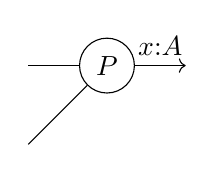
\begin{tikzpicture}
      \graph [nodes={draw}, math nodes,->=o-] {
        { / [coordinate, > "$x_1{:}A_1$"] , / [coordinate] }
        --
        P [circle]
        -> ["$x{:}A$"]
        / [coordinate];
      };
    \end{tikzpicture}

    $\downsquigarrow$

    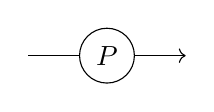
\begin{tikzpicture}
      \graph [nodes={draw}, math nodes] {
        / [coordinate] -- P [circle] -> / [coordinate];
      };
    \end{tikzpicture}
  }

  In data pipelines, the computational processes are arranged in a linear topology, with each process having exactly one upstream provider -- no more and no less.
  To study pipelines, a \enquote{single-provider restriction} is needed -- a type-theoretic analogue of the single-antecedent restriction.
\end{description}


\section{A sequent calculus for propositional singleton logic}\label{sec:singleton-logic:seq-calc}

Having sketched proof-theoretic, category-theoretic, and type-theoretic reasons to investigate the single-antecedent restriction, we now turn to identifying a sequent calculus that satisfies that restriction.

% \subsection{Deriving the sequent calculus rules}\label{sec:singleton-logic:seq-calc:derive}

% The single-antecedent restriction described above
% The sequents of singleton logic have exactly one consequent and, more characteristically, exactly one antecedent: $\slseq{A |- B}$ instead of $\oseq{\octx |- B}$.

% In addition to providing sequents with this elegant symmetry, the single-antecedent restriction is also natural from a category-theoretic perspective.
% In a category, each morphism $f\colon X \rightarrow Y$ has exactly one object -- no more and no less -- as its domain.
% Because sequents should represent a kind of function, single antecedents are just as natural as single object domains.

% Once we impose the single-antecedent restriction upon sequents, all of the rules from the sequent calculus for intuitionistic ordered logic must be reconsidered.

\newthought{One approach} to constructing a singleton sequent calculus is to take the intuitionistic ordered sequent calculus of \cref{??}, apply the single-antecedent restriction to each rule's sequents, and solve the constraints that that restriction imposes.
% upon the ordered sequent calculus's rules.

For instance, consider the ordered cut rule (see neighboring display).
%
\begin{marginfigure}[8.5\baselineskip]
  \normalsize
  \vspace*{-\abovedisplayskip}
  \begin{gather*}
    \infer[\jrule{CUT}^B]{\oseq{\octx'_L \oc \octx \oc \octx'_R |- C}}{
      \oseq{\octx |- B} & \oseq{\octx'_L \oc B \oc \octx'_R |- C}}
    \\
    \mathord{\downsquigarrow}\hspace{5pt}\hphantom{\jrule{CUT}^B}
    \\
    \infer[\jrule{CUT}^B]{\slseq{A |- C}}{
      \slseq{A |- B} & \slseq{B |- C}}
  \end{gather*}
  \caption{Deriving the singleton sequent calculus's cut rule from the corresponding ordered sequent calculus rule}\label{fig:singleton-logic:seq-calc:derive-cut}
\end{marginfigure}
%
% \begin{equation*}
%   \infer[\jrule{CUT}^B]{\oseq{\octx'_L \oc \octx \oc \octx'_R |- C}}{
%     \oseq{\octx |- B} & \oseq{\octx'_L \oc B \oc \octx'_R |- C}}
% \end{equation*}
For the first premise to satisfy the single-antecedent restriction, the finitary context $\octx$ must be exactly a single antecedent, $A$.
Because the second premise already contains the antecedent $B$, the contexts $\octx'_L$ and $\octx'_R$ must also be empty.
After these revisions, the rule contains only well-formed singleton sequents and is a candidate for inclusion in the singleton sequent calculus.

% With these revisions, all sequents of the resulting rule are well-formed singleton sequents, 


% Because the second premise already contains the antecedent $B$, the contexts $\octx'_L$ and $\octx'_R$ must be empty if the premise is to satisfy the single-antecedent restriction.
% % Under this constraint, the cut principle becomes:
% % \begin{equation*}
% %   \infer[\jrule{CUT}^B]{\oseq{\octx'_L \oc \octx \oc \octx'_R |- C}}{
% %     \oseq{\octx |- B} & \oseq{\octx'_L \oc B \oc \octx'_R |- C}}
% %   \rightsquigarrow
% %   \infer{\oseq{\octx |- C}}{
% %     \oseq{\octx |- B} & \oseq{B |- C}}
% % \end{equation*}
% We then replace the finitary context $\octx$ with a single antecedent, $A$, so that the rule's first premise and conclusion also satisfy the [characteristic] restriction.
% All sequents of the resulting rule are well-formed, making it a candidate for inclusion in the singleton sequent calculus.
% % \begin{equation*}
% %   \begin{array}{@{}ccl@{}}
% %     \text{\scshape ordered logic} && \text{\scshape singleton logic}
% %     \\[3\jot]
% %     \infer[\jrule{CUT}^B]{\oseq{\octx'_L \oc \octx \oc \octx'_R |- C}}{
% %       \oseq{\octx |- B} & \oseq{\octx'_L \oc B \oc \octx'_R |- C}}
% %   % \rightsquigarrow
% %   % \infer{\oseq{\octx |- C}}{
% %   %   \oseq{\octx |- B} & \oseq{B |- C}}
% %     & \rightsquigarrow &
% %     \infer[\jrule{CUT}^B]{\slseq{A |- C}}{
% %       \slseq{A |- B} & \slseq{B |- C}}
% %   \end{array}
% % \end{equation*}
% % We could equally well justify this cut rule for singleton logic by first principles, as it expresses the composition of two well-formed sequents\alertinline{proofs?} in singleton logic.

We could equally well justify this new cut rule by first principles, as it expresses the composition of two well-formed singleton sequents [proofs?].
But the above method of considering the constraints imposed by the single-antecedent restriction is a straightforward, mechanical way ahead for the other inference rules.
For example, singleton sequent calculus rules for additive disjunction may also be constructed in this way\parencref[see]{fig:singleton-logic:seq-calc:derive-plus}.
%
\begin{figure*}[tbp]
  \captionsetup{captionskip=0pt,farskip=0pt,nearskip=0pt}
  \vspace*{-\abovecaptionskip}
  
  $\begin{array}{@{}l@{}ccc@{}}
    & \text{\itshape Ordered sequent calculus} && \text{\itshape Singleton sequent calculus}
    \\
%    \subfloat[\label{fig:singleton-logic:seq-calc:derive-cut}]{\quad}
    % &
    % \infer[\mathrlap{\jrule{CUT}^B}]{\oseq{\octx'_L \oc \octx \oc \octx'_R |- C}}{
    %   \oseq{\octx |- B} & \oseq{\octx'_L \oc B \oc \octx'_R |- C}}
    % &
    % \mathrel{\phantom{\rrule{\plus}_2}\mathord{\rightsquigarrow}}
    % &
    % \infer[\mathrlap{\jrule{CUT}^B}]{\slseq{A |- C}}{
    %   \slseq{A |- B} & \slseq{B |- C}}      
    % \\
%    \subfloat[\label{fig:singleton-logic:seq-calc:derive-plus}]{\quad}
    &\!
    \begin{gathered}[t]
      \infer[\rrule{\plus}_1]{\oseq{\octx |- B_1 \plus B_2}}{
        \oseq{\octx |- B_1}}
      \quad
      \infer[\mathrlap{\rrule{\plus}_2}]{\oseq{\octx |- B_1 \plus B_2}}{
        \oseq{\octx |- B_2}}
      \\
      \infer[\mathrlap{\lrule{\plus}}]{\oseq{\octx'_L \oc (B_1 \plus B_2) \oc \octx'_R |- C}}{
        \oseq{\octx'_L \oc B_1 \oc \octx'_R |- C} &
        \oseq{\octx'_L \oc B_2 \oc \octx'_R |- C}}
    \end{gathered}
    &
    \mathrel{\phantom{\rrule{\plus}_2}\mathord{\rightsquigarrow}}
    &\!
    \begin{gathered}[t]
      \infer[\rrule{\plus}_1]{\slseq{A |- B_1 \plus B_2}}{
        \slseq{A |- B_1}}
      \quad
      \infer[\mathrlap{\rrule{\plus}_2}]{\slseq{A |- B_1 \plus B_2}}{
        \slseq{A |- B_2}}
      \\
      \infer[\mathrlap{\lrule{\plus}}]{\slseq{B_1 \plus B_2 |- C}}{
        \slseq{B_1 |- C} & \slseq{B_2 |- C}}
    \end{gathered}
  \end{array}$
  \caption{Deriving the singleton sequent calculus rules for \protect\subref{fig:singleton-logic:seq-calc:derive-cut}~cut and \protect\subref{fig:singleton-logic:seq-calc:derive-plus}~additive disjunction from the corresponding ordered sequent calculus rules}\label{fig:singleton-logic:seq-calc:derive}
\end{figure*}
%
Rules for the other additive connectives ($\with$, $\top$, and $\zero$) can be constructed, too, but we will momentarily postpone displaying them.
% Similarly, the other additive connectives ($\with$, $\top$, and $\zero$) can be given singleton sequent calculus rules.

\newthought{%
However, not all} ordered logical connectives fare as well under the single-antecedent restriction as the additive connectives do.
In particular, the multiplicative connectives do not have analogues in singleton logic.
[, precisely because their multiplicative nature involves splitting antecedents among several premises and, in other rules, extending the context with additional antecedents.]

\begin{marginfigure}[12\baselineskip]
  \normalsize
  \begin{gather*}
    \infer[\rrule{\limp}]{\oseq{\octx |- B_1 \limp B_2}}{
      \oseq{B_1 \oc \octx |- B_2}}
    \\
    \mathord{\downsquigarrow}\hspace{5pt}\hphantom{\rrule{\limp}}
    \\
    \infer[\rrule{\limp}\mathrlap{?}]{\slseq{A |- B_1 \limp B_2}}{
      \slseq{B_1 \oc A |- B_2}}
    \\
    \mathord{\downsquigarrow}\hspace{5pt}\hphantom{\rrule{\limp}}
    \\
    \infer[\rrule{\limp}\mathrlap{?}]{\slseq{A |- B_1 \limp B_2}}{
      \slseq{B_1 \fuse A |- B_2}}
  \end{gather*}
  \caption{A failed attempt at constructing a right rule for left-handed implication}\label{fig:singleton-logic:seq-calc:derive-limp}
\end{marginfigure}
%
Consider, for example, left-handed implication and its right rule (see neighboring \lcnamecref{fig:singleton-logic:seq-calc:derive-limp}).
% \begin{equation*}
%   \infer[\rrule{\limp}]{\oseq{\octx |- B_1 \limp B_2}}{
%     \oseq{B_1 \oc \octx |- B_2}}
% \end{equation*}
The finitary context $\octx$ must be replaced with a single antecedent, $A$, if the rule's conclusion is to be a well-formed singleton sequent.
% \begin{equation*}
%   \infer[\rrule{\limp}]{\oseq{\octx |- B_1 \limp B_2}}{
%     \oseq{B_1 \oc \octx |- B_2}}
%   \rightsquigarrow
%   \infer[\rrule{\limp}?]{\oseq{A |- B_1 \limp B_2}}{
%     \oseq{B_1 \oc A |- B_2}}
% \end{equation*}
Now the revised rule's conclusion is well-formed, but its premise is not.

From a category-theoretic perspective, it would be quite natural to rewrite the premise using ordered conjunction so that the two antecedents are packaged together as one.
% \begin{equation*}
%   \infer[\rrule{\limp}?]{\slseq{A |- B_1 \limp B_2}}{
%     \slseq{B_1 \fuse A |- B_2}}
% \end{equation*}
% 
% Viewed through a category-theoretic lens, this rule is quite innocuous, even natural.
However, from a proof-theoretic perspective, this rule is not suitable -- with this rule, the meaning of left-handed implication depends on the meaning of another connective, namely multiplicative conjunction.
% From a proof-theoretic perspective, however, the meaning of a logical connective should be independent from other connectives, and this rule creates an objectionable dependence of left-handed implication upon ordered conjunction.
As a practical consequence, the subformula property and related cut elimination theorem would fail to hold if the singleton sequent calculus adopted this rule.

In trying to construct singleton sequent calculus rules for left-handed implication, the fundamental problem is that the $\rrule{\limp}$ rule introduces an additional antecedent to a context that is, and must remain, a singleton.
Changing the size of the context by introducing, or sometimes removing, antecedents is an essential characteristic of multiplicative connectives, and so the multiplicative connectives, by their very nature, cannot appear in singleton logic.

% The left rule for left-handed implication is equally problematic:
% \begin{equation*}
%   \infer[\lrule{\limp}]{\oseq{\octx_L \oc \octx \oc (B_1 \limp B_2) \oc  \octx_R |- C}}{
%     \oseq{\octx |- B_1} & \oseq{\octx_L \oc B_2 \oc \octx_R |- C}}
%   \rightsquigarrow
%   \infer[\lrule{\limp}?]{\slseq{A \oc (B_1 \limp B_2) |- C}}{
%     \slseq{A |- B_1} & \slseq{B_2 |- C}}
% \end{equation*}

% Attempting to give singleton calculus rules for the other multiplicative connectives fails similarly.







% \begin{marginfigure}
%   \normalsize
%   \begin{inferences}
%     \infer[\lrule{\limp}?]{\slseq{A \oc (B_1 \limp B_2) |- C}}{
%       \slseq{A |- B_1} & \slseq{B_2 |- C}}
%   \end{inferences}
%   \caption{A left rule for left-handed implication is equally problematic.}
% \end{marginfigure}

% \begin{inferences}
%   \infer[\rrule{\fuse}?]{\slseq{A_1 \fuse A_2 |- B_1 \fuse B_2}}{
%     \slseq{A_1 |- B_1} & \slseq{A_2 |- B_2}}
%   \and
%   \infer[\lrule{\fuse}?]{\slseq{B_1 \fuse B_2 |- C}}{
%     \slseq{B_1 \fuse B_2 |- C}}
% \end{inferences}

% \subsection{A sequent calculus for propositional singleton logic}\label{sec:singleton-logic:seq-calc:full}

\newthought{%
\Cref{fig:singleton-logic:seq-calc}} presents the complete set of rules for propositional singleton logic's sequent calculus.
%
\begin{figure}[tbp]
  \vspace*{\dimexpr-\abovedisplayskip-\abovecaptionskip\relax}
  \begin{syntax*}
    Propositions &
      A,B,C & \alpha \mid A \plus B \mid \zero \mid A \with B \mid \top
  \end{syntax*}
  \begin{inferences}
    \infer[\jrule{CUT}^B]{\slseq{A |- C}}{
      \slseq{A |- B} & \slseq{B |- C}}
    \and
    \infer[\jrule{ID}^A]{\slseq{A |- A}}{}
    \\
    \infer[\rrule{\plus}_1]{\slseq{A |- B_1 \plus B_2}}{
      \slseq{A |- B_1}}
    \and
    \infer[\rrule{\plus}_2]{\slseq{A |- B_1 \plus B_2}}{
      \slseq{A |- B_2}}
    \and
    \infer[\lrule{\plus}]{\slseq{B_1 \plus B_2 |- C}}{
      \slseq{B_1 |- C} & \slseq{B_2 |- C}}
    \\
    \text{(no $\rrule{\zero}$ rule)}
    \and
    \infer[\lrule{\zero}]{\slseq{\zero |- C}}{}
    \\
    \infer[\rrule{\with}]{\slseq{A |- B_1 \with B_2}}{
      \slseq{A |- B_1} & \slseq{A |- B_2}}
    \and
    \infer[\lrule{\with}_1]{\slseq{B_1 \with B_2 |- C}}{
      \slseq{B_1 |- C}}
    \and
    \infer[\lrule{\with}_2]{\slseq{B_1 \with B_2 |- C}}{
      \slseq{B_2 |- C}}
    \\
    \infer[\rrule{\top}]{\slseq{A |- \top}}{}
    \and
    \text{(no $\lrule{\top}$ rule)}
  \end{inferences}
  \vspace*{-\belowdisplayskip}
  \caption{A sequent calculus for propositional singleton logic\label{fig:singleton-logic:seq-calc}}
\end{figure}
%
% The well-formed propositions are exactly the additive propositions of ordered logic, and the complete set of inference rules has been derived from those of the ordered sequent calculus by 

% There is an important observation to be made here.
Although the propositions of singleton logic are exactly the additive propositions of ordered logic, singleton logic is \emph{not} the additive fragment of ordered logic.
For instance, the sequent $\oseq{A \oc B |- \top}$ is provable in the additive fragment of ordered logic, but it
% $\slseq{A \oc B |- \top}$
is not even a well-formed sequent in the singleton sequent calculus [, for the simple reason that it violates the single-antecedent restriction].

That said, singleton logic only differs from the additive fragment of ordered logic in its treatment of $\zero$ and $\top$ -- the $\zero$,$\top$-free fragment of singleton logic coincides exactly with the $\zero$,$\top$-free, additive fragment (that is, the $\plus$,$\with$-fragment) of ordered logic.
% 
% That said, the two logics are related once $\zero$ and $\top$ are excluded -- the $\zero,\top$-free fragment of singleton logic is exactly the $\zero,\top$-free additive fragment of ordered logic.
% Stated differently, the $\plus,\with$-fragment of singleton sequent calculus coincides with the $\plus,
% 
% That said, if $\top$ and $\zero$ are removed, the remainder of singleton logic is indeed exactly the $\plus,\with$-fragment of ordered logic.
A simple structural induction proves this:
\begin{theorem}
  If\/ $\oseq{\octx |- B}$ in the $\plus$,$\with$-fragment of the ordered sequent calculus, then there exists a proposition $A$ such that $\slseq{\octx = A |- B}$ in the $\plus$,$\with$-frag\-ment of the singleton sequent calculus.
\end{theorem}

[Should I mention problems with $\top$ and $\zero$ and how singleton logic sanitizes them?]

% Second, it is worth reiterating that singleton logic, peculiarly, has no form of implication.
% % as mentioned previously, singleton logic contains no multipicative connectives and, most peculiarly, no form of implication.
% It is odd to contemplate that a logic without an implication connective to internalize the logic's underlying hypothetical judgment could possibly be well-defined.
% But as the metatheoretic results of the following \lcnamecref{sec:singleton-logic:seq-calc:metatheory} verify, singleton sequent caluculus is indeed well-defined, resting on the solid foundation of a verificationist meaning-theory.

\subsection{Metatheory: Cut elimination and identity expansion}\label{sec:singleton-logic:seq-calc:metatheory}

The rules shown in \cref{fig:singleton-logic:seq-calc} certainly have the appearance of sequent calculus rules, but do they truly constitute a well-defined sequent calculus?
Most peculiarly, the singleton sequent calculus has no implication connective that internalizes the underlying hypothetical judgment.
Can such a calculus possibly be well-defined?

Because it coincides exactly with a fragment of the ordered sequent calculus, the singleton sequent calculus is indeed well-defined.
However, for our subsequent development, it will prove useful to examine the singleton sequent calculus's metatheory, especially cut elimination, natively.

\newthought{In the tradition} of \citeauthor{Gentzen:MZ35}, \citeauthor{Dummett:HUP91}, and \citeauthor{Martin-Lof:NJPL96}\autocites{Gentzen:MZ35}{Dummett:HUP91}{Martin-Lof:NJPL96}, a sequent calculus is well-defined if it rests on the solid foundation of a verificationist meaning-explanation.
That is, the meaning of each logical connective must be given entirely by its right [and left inference] rules, and those rules must exist in harmony [with the left rules].%
\alertnote{Right rules only, because it is verificationist?}

A \emph{verification}, then, is a proof that relies only on the right and left inference rules and the $\jrule{ID}^{\alpha}$ rule for propositional variables $\alpha$ -- stated differently, verifications may not contain instances of the $\jrule{CUT}$ or general $\jrule{ID}^A$ rules.

If every proof has a corresponding verification, then we can be sure that neither the $\jrule{CUT}$ nor $\jrule{ID}$ rules play any role in defining the logical connectives.


In the tradition of \citeauthor{Gentzen:??}, \citeauthor{Dummett:??}, and \citeauthor{Martin-Lof:??}\autocites{Gentzen:??}{Dummett:??}{Martin-Lof:??}, a sequent calculus is well-defined if it rests on the solid foundation of a verificationist meaning-theory.
That is, the meaning of each logical connective must be given entirely by its right [and left inference] rules, and those rules must exist in harmony [with the left rules].%
\alertnote{Right rules only, because it is verificationist?}

In \citeauthor{Martin-Lof:??}'s words, the meaning of a logical connective must be given by what counts as a verification of it.
A \emph{verification}, then, is a proof that relies only on the right and left inference rules and the $\jrule{ID}^{\alpha}$ rule for propositional variables $\alpha$ -- stated differently, verifications may not contain instances of the $\jrule{CUT}$ or general $\jrule{ID}^A$ rules.


For this program to succeed, we need to be sure that for every proof there is a corresponding verification -- we need a weak 

In this sense, the usual cut elimination metatheorem states a weak normalization result.
%
\begin{theorem}[Cut elimination]\label{thm:singleton-logic:seq-calc:cut-elimination}
  If a proof of $\slseq{A |- C}$ exists, then there exists a cut-free proof of $\slseq{A |- C}$.
\end{theorem}
%
As usual, the cut elimination \lcnamecref{thm:singleton-logic:seq-calc:cut-elimination} may be proved by a straightforward induction on the structure of the given proof, provided that a cut principle for cut-free proofs is admissible:
% 
\begin{lemma*}[Admissibility of cut]\label{lem*:singleton-logic:seq-calc:cut-admissibility}
  If cut-free proofs of $\slseq{A |- B}$ and $\slseq{B |- C}$ exist, then there exists a cut-free proof of $\slseq{A |- C}$.
\end{lemma*}

\newthought{Before proceeding} to this \lcnamecref{lem:singleton-logic:seq-calc:cut-admissibility}'s proof, it is worth emphasizing a subtle distinction between the singleton sequent calculus's primitive $\jrule{CUT}$ rule and the admissible cut principle that this \lcnamecref{lem:singleton-logic:seq-calc:cut-admissibility} establishes.

To be completely formal, we could treat cut-freeness as an extrinsic, Curry-style property of proofs%
\footnote{Contrast this with a separate, intrinsically cut-free sequent calculus in the style of Church \parencite{Pfenning:Andrews??}.}
and indicate cut-freeness by decorating the turnstile: $\cfslseq{A |- C}$ is a cut-free proof of $\slseq{A |- C}$.
The admissible cut principle stated in \cref{lem:singleton-logic:seq-calc:cut-admissibility} could then be expressed as the rule
\begin{equation*}
  \infer-[\jrule{A-CUT}\smash{^B}]{\cfslseq{A |- C}}{
    \cfslseq{A |- B} & \cfslseq{B |- C}}
  ,
\end{equation*}
with the dotted line indicating that it is an admissible, not primitive, rule.
Writing it in this way emphasizes that proving \cref{lem:singleton-logic:seq-calc:cut-admissibility} amounts to defining a meta-level function that takes cut-free proofs of $\slseq{A |- B}$ and $\slseq{B |- C}$ and produces a \emph{cut-free} proof of $\slseq{A |- C}$.
% Moreover, the decorated turnstile makes it clear that all three proofs are cut-free by construction.
% 
Contrast this with the primitive $\jrule{CUT}$ rule of the singleton sequent calculus%
\marginnote[-.5\baselineskip]{
  \normalsize
  $\infer[\jrule{CUT}\smash{^B}]{\slseq{A |- C}}{
     \slseq{A |- B} & \slseq{B |- C}}$%
}%
, which forms a (cut-full) proof of $\slseq{A |- C}$ from (potentially cut-full) proofs of $\slseq{A |- B}$ and $\slseq{B |- C}$.
% \footnote{Which are not necessarily cut-free.}.

From here on, we won't bother to be quite so pedantic, instead often omitting the turnstile decoration on cut-free proofs with the understanding that the admissible $\jrule{A-CUT}$ rule may only be applied to cut-free proofs.

%  writing the admissible cut principle as
% \begin{equation*}
%   \infer-[\jrule{A-CUT}^B]{\slseq{A |- C}}{
%     \slseq{A |- B} & \slseq{B |- C}}
% \end{equation*}
% with the understanding that this admissible rule may only be applied to cut-free proofs.


\newthought{With that} clarification out of the way, we are finally ready to prove the admissibility of cut \lcnamecref{lem:singleton-logic:cut-admissibility}.

\begin{lemma}[Admissibility of cut]\label{lem:singleton-logic:cut-admissibility}
  If cut-free proofs of $\slseq{A |- B}$ and $\slseq{B |- C}$ exist, then there exists a cut-free proof of $\slseq{A |- C}$.
\end{lemma}
%
\begin{proof}
  Just as in the proof of admissibility of cut for the ordered sequent calculus\parencref{lem:ordered-logic:cut-admissibility}, we use a standard lexicographic structural induction, first on the structure of the cut formula, and then on the structures of the given proofs.

  As usual, the cases can be classified into three categories: principal cases, identity cases, and commutative cases.
  % We show a few sample cases.
  \begin{description}[listparindent=\parindent, parsep=0pt]
  \item[Principal cases]
    As usual, the principal cases pair a proof ending in a right rule together with a proof ending in a corresponding left rule.
    % , so that the last inference of each proof introduces the cut formula.
    % For example, one of the principal cases pairs a proof ending in the $\rrule{\plus}_1$ rule with one ending in the $\lrule{\plus}$ rule; it is resolved as follows.
    One such principal case is:
    \begin{gather*}
      \infer-[\jrule{A-CUT}\smash{^{B_1 \plus B_2}}]{\slseq{A |- C}}{
        \infer[\rrule{\plus}_1]{\slseq{A |- B_1 \plus B_2}}{
          \deduce{\slseq{A |- B_1}}{\DD_1}} &
        \infer[\lrule{\plus}]{\slseq{B_1 \plus B_2 |- C}}{
          \deduce{\slseq{B_1 |- C}}{\EE_1} &
          \deduce{\slseq{B_2 |- C}}{\EE_2}}}
      % 
      \\=\\
      % 
      \infer-[\jrule{A-CUT}\smash{^{B_1}}]{\slseq{A |- C}}{
        \deduce{\slseq{A |- B_1}}{\DD_1} &
        \deduce{\slseq{B_1 |- C}}{\EE_1}}
      \qquad
    \end{gather*}
    Notice that the interaction between proofs here is synchronous -- the case is resolved by appealing to the inductive hypothesis at a smaller cut formula.
  
  \item[Identity cases]
    In the identity cases, one of the proofs is the $\jrule{ID}$ rule alone.
    For example:
    % One of the identity cases pairs the $\jrule{ID}$ rule with a proof of $\slseq{A |- C}$:
    \begin{equation*}
      \infer-[\jrule{A-CUT}\smash{^A}]{\slseq{A |- C}}{
        \infer[\jrule{ID}\smash{^A}]{\slseq{A |- A}}{} &
        \deduce{\slseq{A |- C}}{\EE}}
      % 
      \quad=\quad
      % 
      \deduce{\slseq{A |- C}}{\EE}
      \,.
    \end{equation*}
    % That $\jrule{CUT}$ and $\jrule{ID}$ are inverses here is consistent with the idea that the cut and identity principles are dual.
    
  \item[Commutative cases]
    As in the proof of ordered logic's admissible cut principle\parencref{lem:ordered-logic:cut-admissibility}, the commutative cases are those in which one of the proofs ends by introducing a side formula.
    % the last inference in one of the proofs introduces a formula other than the cut formula;
    % the cases are subcategorized as left- or right-commutative according to the proof involved.
    % In both scenarios, the cut and involved inference rule commute, with an appeal to the inductive hypothesis at the same cut formula but smaller proofs.

    % % The left commutative cases pair a proof of $\slseq{A |- B}$ ending in a left rule together with a proof of $\slseq{B |- C}$.
    % For example, one left-commutative case
    % % of the left commutative cases
    % pairs a proof of $\slseq{A_1 \plus A_2 |- B}$ ending in the $\lrule{\plus}$ rule together with a proof of $\slseq{B |- C}$:
    % \begin{gather*}
    %   \infer-[\mathrlap{\jrule{A-CUT}\smash{^B}}]{\slseq{A_1 \plus A_2 |- C}}{
    %     \infer[\lrule{\plus}]{\slseq{A_1 \plus A_2 |- B}}{
    %       \deduce{\slseq{A_1 |- B}}{\DD_1} &
    %       \deduce{\slseq{A_2 |- B}}{\DD_2}} &
    %     \deduce{\slseq{B |- C}}{\EE}}
    %   % 
    %   \\=\\
    %   % 
    %   \infer[\lrule{\plus}]{\slseq{A_1 \plus A_2 |- C}}{
    %     \infer-[\jrule{A-CUT}\smash{^B}]{\slseq{A_1 |- C}}{
    %       \deduce{\slseq{A_1 |- B}}{\DD_1} &
    %       \deduce{\slseq{B |- C}}{\EE}} &
    %     \infer-[\mathrlap{\jrule{A-CUT}\smash{^B}}]{\slseq{A_2 |- C}}{
    %       \deduce{\slseq{A_2 |- B}}{\DD_2} &
    %       \deduce{\slseq{B |- C}}{\EE}}}
    % \end{gather*}

  % \item[Right commutative cases]
    % The right commutative cases pair a proof of $\slseq{A |- B}$ together with a proof of $\slseq{B |- C}$ ending in a right rule.
    % For example, one such case
    As an example, one right-commutative case
    % of the right commutative cases
    pairs a proof of $\slseq{A |- B}$ with a proof of $\slseq{B |- C_1 \plus C_2}$ ending in the $\rrule{\plus}_1$ rule:
    % ; it is resolved as follows.
    \begin{equation*}
      \infer-[\jrule{A-CUT}\smash{^B}]{\slseq{A |- C_1 \plus C_2}}{
        \deduce{\slseq{A |- B}}{\DD} &
        \infer[\rrule{\plus}_1]{\slseq{B |- C_1 \plus C_2}}{
          \deduce{\slseq{B |- C_1}}{\EE_1}}}
      % 
      \quad=\quad
      % 
      \infer[\rrule{\plus}_1]{\slseq{A |- C_1 \plus C_2}}{
        \infer-[\jrule{A-CUT}\smash{^B}]{\slseq{A |- C_1}}{
          \deduce{\slseq{A |- B}}{\DD} &
          \deduce{\slseq{B |- C_1}}{\EE_1}}}
    \end{equation*}
    Unlike in ordered logic, there can be no right-commutative cases involving left rules because the cut formula is the only antecedent in the sequent $\slseq{B |- C}$.
    % In this way, the proof of admissibility of cut for the singleton sequent calculus is more symmetric than that of the ordered sequent calculus.
    In this way, the symmetry of singleton sequents is manifest even in proving the admissibility of cut.
    \qedhere
  \end{description}
\end{proof}


\newthought{With the admissibility} of cut established, we can finally prove cut elimination for the singleton sequent calculus.
%
\begin{theorem}[Cut elimination]
  If a proof of $\slseq{A |- C}$ exists, then a cut-free proof of $\slseq{A |- C}$ exists.
\end{theorem}
%
\begin{proof}
  By structural induction on the proof of $\slseq{A |- C}$, appealing to the admissibility of cut\parencref{lem:singleton-logic:seq-calc:cut-admissibility} when encountering a $\jrule{CUT}$ rule.

  If we display the inductive hypothesis as an admissible rule, then the crucial case in the proof of cut elimination is resolved as follows.
  \begin{equation*}
    \infer-[\jrule{CE}]{\cfslseq{A |- C}}{
      \infer[\jrule{CUT}\smash{^B}]{\slseq{A |- C}}{
        \deduce{\slseq{A |- B}}{\DD_1} & \deduce{\slseq{B |- C}}{\DD_2}}}
    \quad=\quad
    \infer-[\jrule{A-CUT}\smash{^B}]{\cfslseq{A |- C}}{
      \infer-[\jrule{CE}]{\cfslseq{A |- B}}{
        \deduce{\slseq{A |- B}}{\DD_1}} &
      \infer-[\jrule{CE}]{\cfslseq{B |- C}}{
        \deduce{\slseq{B |- C}}{\DD_2}}}
  \end{equation*}
  All other cases are handled compositionally.

  This proof amounts to defining a meta-level function for normalizing proofs to cut-free form.
\end{proof}



\section{A Hilbert-style axiomatization of singleton logic}\label{sec:singleton-logic:hilbert}

Sequent calculi are not the only way to present logics, so
% natural deduction calculi and Hilbert systems are also commonly used, for instance.
in this \lcnamecref{sec:singleton-logic:hilbert} we also consider a Hilbert-style axiomatization of singleton logic.
Our interest in a Hilbert system for singleton logic is not taxonomic, however.
Rather, over the course of the next \lcnamecref{ch:process-chains} and a half, we shall see that normalization of Hilbert-style proofs serves as the basis of a Curry--Howard isomorphism with chains of asynchronously communicating processes.

% \subsection{A Hilbert-style axiomatization of linear logic}

\newthought{In a sequent calculus}, the meaning of a connective is given by its right and left inference rules.
Hilbert-style axiomatizations, on the other hand, strive to use as few rules of inference as possible, with the meaning of a connective instead given by a small collection of axiom schemas.

The term \enquote*{axiom schema} is often interpreted narrowly to mean only categorical judgments like $\vdash A \imp B \imp A \land B$, not hypothetical judgments like $\ctx , A , B \vdash A \land B$ adopted as zero-premise rules of inference.
Consequently, Hilbert-style axiomatizations usually rely heavily on implication and a \emph{modus ponens} rule
%
\begin{marginfigure}
  \begin{equation*}
    \infer[\jrule{MP}]{\vdash B}{
      \vdash A \imp B & \vdash A}
  \end{equation*}
  \caption{\emph{Modus ponens} for a Hilbert-style axiomatization of intuitionistic logic}
\end{marginfigure}%
%
to effect the meanings of the logical connectives.

However, as explained in \cref{??}, singleton logic does not enjoy the luxury of an implication connective.
So in a Hilbert-style axiomatization of singleton logic, we will have to content ourselves with a broad interpretation of the term \enquote*{axiom schema} that encompasses zero-premise rules.

\newthought{To construct} a Hilbert-style axiomatization of singleton logic, we will ask, in turn, whether each sequent calculus rule can be reduced to an axiom schema.

First, consider the judgmental rules, $\jrule{ID}$ and $\jrule{CUT}$, for the identity and cut principles (see neighboring display).%
\marginnote{%
  \begin{inferences}
    \infer[\mathrlap{\jrule{ID}^A}]{\slseq{A |- A}}{}
    \hphantom{\jrule{CUT}^B}
    \\
    \infer[\mathrlap{\jrule{CUT}^B}]{\slseq{A |- C}}{
      \slseq{A |- B} & \slseq{B |- C}}
    \hphantom{\jrule{CUT}^B}
  \end{inferences}
}
With zero premises, the $\jrule{ID}$ rule itself is already an axiom schema and can be adopted directly in singleton logic's Hilbert system.

The $\jrule{CUT}$ rule is not quite so accommodating.
As a rule for composing proofs, the $\jrule{CUT}$ rule serves a similar purpose to the traditional \emph{modus ponens} rule.
Just as \emph{modus ponens} cannot be reduced to an axiom schema, so must $\jrule{CUT}$ remain a rule of inference [in our Hilbert system].
Moreover, because singleton logic has no implication connective, the rule's hypothetical judgments cannot even be simplified to categorical judgments.
Therefore, the $\jrule{CUT}$ rule is adopted wholesale in the Hilbert system.

% Because singleton logic does not have an implication connective to internalize the hypothetical judgment, there is no obvious way to turn this rule into an axiom.
% Both rules are therefore adopted wholesale in the Hilbert-style axiomatization.

Next, consider the sequent calculus's $\rrule{\plus}_1$ inference rule.
% ; how much can we push this rule toward an axiom?
Using the $\jrule{ID}$ axiom schema, we can obtain a zero-premise derived rule from $\rrule{\plus}_1$:
\begin{equation*}
  \infer[\rrule{\plus}_1]{\slseq{A_1 |- A_1 \plus A_2}}{
    \infer[\jrule{ID}]{\slseq{A_1 |- A_1}}{}}
  %
  \quad\leftrightsquigarrow\quad
  %
  \infer[\rrule{\plus}'_1]{\slseq{A_1 |- A_1 \plus A_2}}{}
\end{equation*}
Moreover, by combining this new $\rrule{\plus}'_1$ axiom schema with $\jrule{CUT}$, we can recover the original $\rrule{\plus}_1$ rule as a derived rule:
\begin{equation*}
  \infer[\jrule{CUT}]{\slseq{A |- B_1 \plus B_2}}{
    \slseq{A |- B_1} &
    \infer[\rrule{\plus}'_1]{\slseq{B_1 |- B_1 \plus B_2}}{}}
  %
  \quad\leftrightsquigarrow\quad
  %
  \infer[\rrule{\plus}_1]{\slseq{A |- B_1 \plus B_2}}{
    \slseq{A |- B_1}}
\end{equation*}
Together, these two observations suggest that $\rrule{\plus}'_1$ be adopted as an axiom schema in the Hilbert-style axiomatization of singleton logic.
A symmetric $\rrule{\plus}'_2$ axiom schema should be adopted, too.

What about the sequent calculus's $\lrule{\plus}$ rule (see neighboring display)?%
\marginnote{%
  \begin{equation*}
    \infer[\lrule{\plus}]{\slseq{B_1 \plus B_2 |- C}}{
      \slseq{B_1 |- C} &
      \slseq{B_2 |- C}}
  \end{equation*}%
}
Can it also be reduced to an axiom schema?
Once again, singleton logic's lack of an implication connective prevents us from even simplifying the $\lrule{\plus}$ rule's hypothetical judgments to categorical judgments.
Like $\jrule{CUT}$, the sequent calculus's $\lrule{\plus}$ rule is thus adopted wholesale in singleton logic's Hilbert system.
Including the additive $\lrule{\plus}$ rule as a primitive rule of inference is perhaps not unexpected.
It is consistent with Hilbert-style axiomatizations of linear logic\autocite{Avron:TCS88}, which include an adjunction rule -- essentially the linear sequent calculus's $\rrule{\with}$ rule -- to effect the additive behavior that linear implication and its multiplicative \emph{modus ponens} rule cannot.

% means that we will just
% Because singleton logic does not have an implication connective to internalize the hypothetical judgment, there is really no way to turn this rule into an axiom.
% Instead, we will
% carry the $\lrule{\plus}$ sequent calculus rule over to our Hilbert-style axiomatization [of singleton logic] as a primitive rule of inference.

The axiomatization of additive conjunction is dual to that of $A_1 \plus A_2$:
The sequent calculus's $\rrule{\with}$ rule will be adopted wholesale, and $\lrule{\with}'_1$ and $\lrule{\with}'_2$ axiom schemas will be derived from the sequent calculus's $\lrule{\with}_1$, $\lrule{\with}_2$, and $\jrule{ID}$ rules.
%
\begin{marginfigure}
  \begin{inferences}
    \infer[\rrule{\with}]{\slseq{A |- C_1 \with C_2}}{
      \slseq{A |- C_1} &
      \slseq{A |- C_2}}
    \\
    \infer[\lrule{\with}'_1]{\slseq{C_1 \with C_2 |- C_1}}{}
    \and
    \infer[\lrule{\with}'_2]{\slseq{C_1 \with C_2 |- C_2}}{}
  \end{inferences}
  \caption{A Hilbert-style axiomatization of additive conjunction from singleton logic}
\end{marginfigure}%
%
And finally, the axiomatizations of $\zero$ and $\top$ are the nullary analogues of those of the binary $\plus$ and $\with$ connectives, respectively.

\Cref{fig:singleton-logic:hilbert} summarizes this Hilbert-style axiomatization of singleton logic.
%
\begin{figure}[tbp]
  \vspace*{\dimexpr-\abovedisplayskip-\abovecaptionskip\relax}
  \begin{syntax*}
    Propositions &
      A & \alpha \mid A \plus B \mid \zero \mid A \with B \mid \top
  \end{syntax*}
  \begin{inferences}
    \infer[\jrule{CUT}^B]{\slseq{A |- C}}{
      \slseq{A |- B} & \slseq{B |- C}}
    \and
    \infer[\jrule{ID}^A]{\slseq{A |- A}}{}
    \\
    \infer[\rrule{\plus}_1']{\slseq{A_1 |- A_1 \plus A_2}}{}
    \and
    \infer[\rrule{\plus}_2']{\slseq{A_2 |- A_1 \plus A_2}}{}
    \and
    \infer[\lrule{\plus}]{\slseq{A_1 \plus A_2 |- C}}{
      \slseq{A_1 |- C} & \slseq{A_2 |- C}}
    \\
    \text{(no $\rrule{\zero}$ rule)}
    \and
    \infer[\lrule{\zero}]{\slseq{\zero |- C}}{}
    \\
    \infer[\rrule{\with}]{\slseq{A |- C_1 \with C_2}}{
      \slseq{A |- C_1} & \slseq{A |- C_2}}
    \and
    \infer[\lrule{\with}_1']{\slseq{C_1 \with C_2 |- C_1}}{}
    \and
    \infer[\lrule{\with}_2']{\slseq{C_1 \with C_2 |- C_2}}{}
    \\
    \infer[\rrule{\top}]{\slseq{A |- \top}}{}
    \and
    \text{(no $\lrule{\top}$ rule)}
  \end{inferences}
  \vspace{-\belowdisplayskip}
  \caption{A Hilbert system for singleton logic}%
  \label{fig:singleton-logic:hilbert}
\end{figure}

% \newthought{In a sequent calculus}, the meaning of a connective is given by its right and left inference rules.
% Hilbert-style axiomatizations, on the other hand, strive to use as few rules of inference as possible, with the meaning of a connective instead given by a small collection of axioms.
% % For example, the neighboring display shows a possible axiomatization of intuitionistic conjunction.%
% % \marginnote{%
% %   $\begin{lgathered}
% %     \vdash A \imp B \imp A \land B \\
% %     \vdash (A \land B \imp A \imp C) \imp (A \land B \imp C) \\
% %     \vdash (A \land B \imp B \imp C) \imp (A \land B \imp C)
% %   \end{lgathered}$
% % }

% The term \enquote*{axiom} is often interpreted narrowly to mean only categorical judgments [logical tautologies?] like $\vdash A \imp B \imp A \land B$, not hypothetical judgments like $\ctx , A , B \vdash A \land B$ adopted as zero-premise rules of inference.
% Consequently, Hilbert-style axiomatizations rely heavily on implication and a \emph{modus ponens} rule to effect the maximum ...

% Although categorical axioms are usually preferred, they are equivalent to the hypothetical axioms.
% The deduction theorem, used to bridge ..., captures this equivalence.
% For example, the following deduction theorem for intuitionistic logic, together with weakening, shows that the categorical axiom $\vdash A \imp B \imp A \land B$ is equivalent to the hypothetical axiom $\ctx , A , B \vdash A \land B$.


% As explained in \cref{??}, singleton logic does not have the luxury of an implication connective, so in a Hilbert-style axiomatization, we will have to satisfy ourselves with hypothetical axioms.


% Next, take the sequent calculus's $\rrule{\plus}_1$ inference rule; how much can we push this rule toward an axiom?
% Consider the derived rule obtained from $\rrule{\plus}_1$ and $\jrule{ID}$:
% \begin{equation*}
%   \infer[\rrule{\plus}_1]{\slseq{A_1 |- A_1 \plus A_2}}{
%     \infer[\jrule{ID}]{\slseq{A_1 |- A_1}}{}}
%   %
%   \infer[\rrule{\plus}'_1]{\slseq{A_1 |- A_1 \plus A_2}}{}
% \end{equation*}

% Given a sequent calculus and Hilbert system, we would like to be sure that the sequent- and Hilbert-style meanings of the logical connectives coincide.
% To bridge the gap between the categorical judgment preferred in a Hilbert-style axiomatization and the hypothetical judgment at the heart of a sequent calculus, a hypothetical Hilbert system and accompanying deduction theorem are used.
% The deduction theorem captures the idea that implication embodies a hypothetical judgment as a logical connective.
% For intuitionistic logic, that theorem would be:
% \begin{theorem*}[Deduction theorem]
%   $\ctx , A \vdash B$ if and only if\/ $\ctx \vdash A \imp B$.
% \end{theorem*}


% Although categorical judgments are preferred, a hypothetical Hilbert system 

% Central to this endeavor is often a deduction theorem which shows that implication embodies the logic's underlying hypothetical judgment as a logical connective.
% For example, a Hilbert-style axiomatization of intuitionistic logic would enjoy the following theorem.
% \begin{theorem*}[Deduction theorem]
%   $\ctx , A \vdash B$ if and only if $\ctx \vdash A \imp B$.
% \end{theorem*}
% On the basis of this theorem, 


% As explained in \cref{??}, singleton logic does not have the luxury of an implication connective and consequently no deduction theorem, so the final  in a Hilbert-style axiomatization, we will have to 


% Often, the term \enquote*{axiom} is interpreted narrowly to mean only 
% \begin{equation*}
%   \begin{lgathered}
%     \vdash A \imp B \imp A \land B \\
%     \vdash (A \imp C) \imp (A \land B \imp C) \\
%     \vdash (B \imp C) \imp (A \land B \imp C)
%   \end{lgathered}
% \end{equation*}


% To avoid unnecessarily introducing rules of inference,
% % Most of the time,
% these axioms rely heavily on implication and a \textit{modus ponens} rule to effect ... 

% To avoid unnecessarily introducing rules of inference,
% % Most of the time,
% these axioms rely heavily on implication and a \textit{modus ponens} rule to effect ... 
% For example, in a Hilbert-style axiomatization of intuitionistic ordered logic\autocite{Avron:??}, ordered conjunction is described by the following axioms.
% \begin{equation*}
%   \begin{lgathered}
%     \vdash B \limp (A \limp A \fuse B) \\
%     \vdash (B \limp (A \limp C)) \limp (A \fuse B \limp C)
%   \end{lgathered}
% \end{equation*}
% The axioms are suggestive of the right and left sequent calculus rules for 
% \begin{equation*}
%   \begin{lgathered}
%     \vdash A \lolli B \lolli A \tensor B \\
%     \vdash (A \lolli B \lolli C) \lolli (A \tensor B \lolli C)
%   \end{lgathered}
%   \quad\rightsquigarrow\quad
%   \begin{gathered}
%     \infer{A , B \vdash A \tensor B}{} \\
%     \infer{A \tensor B \vdash C}{
%       A, B \vdash C}
%   \end{gathered}
% \end{equation*}



% % Whereas sequent calculi use many inference rules but few axioms, Hilbert systems shift the balance far in favor of axioms.


% % In a Hilbert system, each logical connective is defined by a collection of axioms.
% % For example, in a Hilbert system for intuitionistic ordered logic, additive disjunction would be defined by three axioms:
% \begin{equation*}
%   \begin{lgathered}
%     \infer[\with]{\vdash A \with B}{
%       \vdash A & \vdash B}
%     \\
%     \vdash \bigl((A \limp B_1) \with (A \limp B_2)\bigr) \limp (A \limp B_1 \with B_2)
%   \end{lgathered}
%   \qquad
%   \begin{lgathered}[b]
%     \vdash A_1 \with A_2 \limp A_1 \\
%     \vdash A_1 \with A_2 \limp A_2
%   \end{lgathered}
% \end{equation*}


% \newcommand*{\approxident}{%
%   \mathrel{\vcenter{\offinterlineskip
%   \hbox{$\sim$}\vskip-.35ex\hbox{$\sim$}\vskip-.35ex\hbox{$\sim$}}}}

% % For reasons better explained in future \lcnamecrefs{ch:singleton-logic}, we need a Curry--Howard interpretation of singleton logic as a session-type system for asynchronous processes.

% Notice that there is more than one way to extend a proof of $\slseq{A |- B_1}$ to a proof of $\slseq{A |- B_1 \plus B_2}$.
% Of course, the most obvious way is to simply apply the $\rrule{\plus}_1$ rule to the given proof.
% Another, less direct way is to cut the given proof against an identity embellished with the $\rrule{\plus}_1$ rule.
% \begin{equation*}
%   \infer[\rrule{\plus}_1]{\slseq{A |- B_1 \plus B_2}}{
%     \slseq{A |- B_1}}
%   \qquad\text{and}\qquad
%   \infer[\jrule{CUT}^{B_1}]{\slseq{A |- B_1 \plus B_2}}{
%     \slseq{A |- B_1} &
%     \infer[\rrule{\plus}_1]{\slseq{B_1 |- B_1 \plus }}{
%       \infer[\jrule{ID}]{\slseq{B_1 |- B_1}}{}}}
% \end{equation*}
% In fact, these proofs do not merely conclude with the same sequent -- these proofs are related by cut reduction:
% \begin{equation*}
%   \infer[\jrule{CUT}^{B_1}]{\slseq{A |- B_1 \plus B_2}}{
%     \slseq{A |- B_1} &
%     \infer[\rrule{\plus}_1]{\slseq{B_1 |- B_1 \plus B_2}}{
%       \infer[\jrule{ID}]{\slseq{B_1 |- B_1}}{}}}
%   \longrightarrow\longrightarrow\enspace
%   \infer[\rrule{\plus}_1]{\slseq{A |- B_1 \plus B_2}}{
%     \slseq{A |- B_1}}
% \end{equation*}
% This suggests that the $\rrule{\plus}_1$-embellished identity may be worthy of special consideration.

% Suppose that we replace the usual $\rrule{\plus}_1$ rule with a new primitive rule that collapses the embellished identity.
% \begin{equation*}
%   \infer[\rrule{\plus}_1]{\slseq{B_1 |- B_1 \plus B_2}}{
%     \infer[\jrule{ID}]{\slseq{B_1 |- B_1}}{}}
%   \rightsquigarrow
%   \infer[\rrule{\plus}_1']{\slseq{B_1 |- B_1 \plus B_2}}{}
% \end{equation*}


% \begin{gather*}
%   \infer[\jrule{CUT}^{B_1 \plus B_2}]{\slseq{A |- C}}{
%     \infer[\jrule{CUT}^{B_1}]{\slseq{A |- B_1 \plus B_2}}{
%       \slseq{A |- B_1} &
%       \infer[\rrule{\plus}_1]{\slseq{B_1 |- B_1 \plus B_2}}{
%         \infer[\jrule{ID}]{\slseq{B_1 |- B_1}}{}}} &
%     \infer[\lrule{\plus}]{\slseq{B_1 \plus B_2 |- C}}{
%       \slseq{B_1 |- C} & \slseq{B_2 |- C}}}
%   \\\equiv\\
%   \infer[\jrule{CUT}^{B_1}]{\slseq{A |- C}}{
%     \slseq{A |- B_1} &
%     \infer[\jrule{CUT}^{B_1 \plus B_2}]{\slseq{B_1 |- C}}{
%       \infer[\rrule{\plus}_1]{\slseq{B_1 |- B_1 \plus B_2}}{
%         \infer[\jrule{ID}]{\slseq{B_1 |- B_1}}{}} &
%       \infer[\lrule{\plus}]{\slseq{B_1 \plus B_2 |- C}}{
%         \slseq{B_1 |- C} & \slseq{B_2 |- C}}}}
%   \\\longrightarrow\longrightarrow\\
%   \infer[\jrule{CUT}^{B_1}]{\slseq{A |- C}}{
%     \slseq{A |- B_1} & \slseq{B_1 |- C}}
% \end{gather*}

% \begin{gather*}
%   \infer[\jrule{CUT}^{B_1 \plus B_2}]{\slseq{A |- C}}{
%     \infer[\rrule{\plus}_1]{\slseq{A |- B_1 \plus B_2}}{
%       \slseq{A |- B_1}} &
%     \infer[\lrule{\plus}]{\slseq{B_1 \plus B_2 |- C}}{
%       \slseq{B_1 |- C} & \slseq{B_2 |- C}}}
%   \\\longrightarrow\\
%   \infer[\jrule{CUT}^{B_1}]{\slseq{A |- C}}{
%     \slseq{A |- B_1} & \slseq{B_1 |- C}}
% \end{gather*}


% \begin{equation*}
%   \selectR{\kay}[P]
%   \approxident
%   \spawn{P}{(\selectR{\kay}[\fwd])}
% \end{equation*}

% \begin{marginfigure}
%   \begin{gather*}
%     \infer[\rrule{\plus}_1]{\slof{A |- \selectR{\kay}[P] : B_1 \plus B_2}}{
%       \slseq{A |- P : B_1}}
%     \\\approxident\\
%     \infer[\jrule{CUT}^{B_1}]{\slseq{A |- \spawn{P}{(\selectR{\kay}[\fwd])} : B_1 \plus B_2}}{
%       \slseq{A |- P : B_1} &
%       \infer[\rrule{\plus}_1]{\slseq{B_1 |- \selectR{\kay}[\fwd] : B_1 \plus B_2}}{
%         \infer[\jrule{ID}]{\slseq{B_1 |- \fwd : B_1}}{}}}
%   \end{gather*}
%   \caption{}
% \end{marginfigure}


  
% \begin{gather*}
%   \begin{lgathered}
%     \spawn{(\selectR{\kay}[P])}{\caseL[\ell \in L]{\ell => Q_{\ell}}}
%       \longrightarrow \spawn{P}{Q_{\kay}}
%     \\
%     \begin{aligned}
%       \MoveEqLeft[.5]
%       \spawn{\bigl(\spawn{P}{(\selectR{\kay}[\fwd])}\bigr)}{\caseL[\ell \in L]{\ell => Q_{\ell}}} \\[-.75\jot]
%         &\equiv \spawn{P}{\bigl(\spawn{(\selectR{\kay}[\fwd])}{\caseL[\ell \in L]{\ell => Q_{\ell}}}\bigr)} \\[-.75\jot]
%         % &\longrightarrow \spawn{P}{(\spawn{\fwd}{Q_{\kay}})} \\[-.75\jot]
%         &\longrightarrow\longrightarrow \spawn{P}{Q_{\kay}}
%     \end{aligned}
%   \end{lgathered}
% \end{gather*}

% % \begin{gather*}
% %   \infer-[\jrule{CUT}^{B_1 \plus B_2}]{\slseq{A |- C}}{
% %     \infer[\rrule{\plus}_1]{\slseq{A |- B_1 \plus B_2}}{
% %       \slseq{A |- B_1}} &
% %     \infer[\lrule{\plus}]{\slseq{B_1 \plus B_2 |- C}}{
% %       \slseq{B_1 |- C} & \slseq{B_2 |- C}}}
% %   =
% %   \infer-[\jrule{CUT}^{B_1}]{\slseq{A |- B_1 \plus B_2}}{
% %     \slseq{A |- B_1} & \slseq{B_1 |- C}}
% %   \\=\\
% %   \infer-[\jrule{CUT}^{B_1 \plus B_2}]{\slseq{A |- C}}{
% %     \infer[\jrule{CUT}^{B_1}]{\slseq{A |- B_1 \plus B_2}}{
% %       \slseq{A |- B_1} &
% %       \infer[\rrule{\plus}_1]{\slseq{B_1 |- B_1 \plus B_2}}{
% %         \infer[\jrule{ID}]{\slseq{B_1 |- B_1}}{}}} &
% %     \infer[\lrule{\plus}]{\slseq{B_1 \plus B_2 |- C}}{
% %       \slseq{B_1 |- C} & \slseq{B_2 |- C}}}
% %   \equiv
% %   \infer-[\jrule{CUT}^{B_1}]{\slseq{A |- C}}{
% %     \slseq{A |- B_1} &
% %     \infer-[\jrule{CUT}^{B_1 \plus B_2}]{\slseq{B_1 |- C}}{
% %       \infer[\rrule{\plus}_1]{\slseq{B_1 |- B_1 \plus B_2}}{
% %         \infer[\jrule{ID}]{\slseq{B_1 |- B_1}}{}} &
% %       \infer[\lrule{\plus}]{\slseq{B_1 \plus B_2 |- C}}{
% %         \slseq{B_1 |- C} & \slseq{B_2 |- C}}}}
% %   \\=\\
% %   \infer-[\jrule{CUT}^{B_1}]{\slseq{A |- C}}{
% %     \slseq{A |- B_1} &
% %     \infer-[\jrule{CUT}^{B_1 \plus B_2}]{\slseq{B_1 |- C}}{
% %       \infer[\jrule{ID}]{\slseq{B_1 |- B_1}}{} &
% %       \slseq{B_1 |- C}}}
% %   \\=\\
% %   \infer-[\jrule{CUT}^{B_1}]{\slseq{A |- C}}{
% %     \slseq{A |- B_1} & \slseq{B_1 |- C}}
% % \end{gather*}


% \begin{equation*}
%   \infer[\rrule{\plus}_1]{\slseq{B_1 |- B_1 \plus B_2}}{
%     \infer[\jrule{ID}]{\slseq{B_1 |- B_1}}{}}
%   \leftrightsquigarrow
%   \infer[\rrule{\plus}_1']{\slseq{B_1 |- B_1 \plus B_2}}{}
% \end{equation*}


% \begin{equation*}
%   \infer[\rrule{\plus}_1]{\slseq{A |- B_1 \plus B_2}}{
%     \slseq{A |- B_1}}
%   \leftrightsquigarrow
%   \infer[\jrule{CUT}^{B_1}]{\slseq{A |- B_1 \plus B_2}}{
%     \slseq{A |- B_1} &
%     \infer[\rrule{\plus}_1']{\slseq{B_1 |- B_1 \plus B_2}}{}}
% \end{equation*}


% \begin{equation*}
%   \infer-[\jrule{CUT}^{A_1}]{\slseq{A_1 |- C}}{
%     \infer[\rrule{\plus}_1']{\slseq{A_1 |- A_1 \plus A_2}}{} &
%     \infer[\lrule{\plus}]{\slseq{A_1 \plus A_2 |- C}}{
%       \deduce{\slseq{A_1 |- C}}{\EE_1} &
%       \deduce{\slseq{A_2 |- C}}{\EE_2}}}
%   \rightsquigarrow
%   \deduce{\slseq{A_1 |- C}}{\EE_1}
% \end{equation*}



% \begin{inferences}
%   \infer[\jrule{MP}]{\slseq{|- C}}{
%     \slseq{|- B} & \slseq{|- B \limp C}}
%   \\
%   \begin{lgathered}
%   \vdash A \limp A
%   \\
%   \vdash A_1 \limp A_1 \plus A_2 \\
%   \vdash A_2 \limp A_1 \plus A_2 \\
%   \vdash (A_2 \limp C) \limp (A_1 \limp C) \limp (A_1 \plus A_2 \limp C)
% \end{lgathered}
% \end{inferences}





\newthought{The Hilbert system} of \cref{fig:singleton-logic:hilbert} shares so many rules with the singleton sequent calculus\parencref{fig:singleton-logic:seq-calc} that it can be viewed as a variant in which each connective's non-invertible rules have been replaced with zero-premise rules.
As such, we should seek to prove the usual sequent calculus metatheorems -- cut elimination and identity expansion -- for this Hilbert-style variant.

Strictly speaking, cut elimination does not hold for the Hilbert system.
As a concrete [counter]example, there is no cut-free Hilbert-style proof of $\slseq{\alpha_2 |- \alpha_1 \plus (\alpha_2 \plus \alpha_3)}$, even though the same sequent is provable using cut:
\begin{equation*}
  \infer[\jrule{CUT}]{\slseq{\alpha |- \top \plus \top}}{
    \infer[\rrule{\top}]{\slseq{\alpha |- \top}}{} &
    \infer[\rrule{\plus}'_1]{\slseq{\top |- \top \plus \top}}{}}
\end{equation*}
\begin{equation*}
  \infer[\jrule{CUT}]{\slseq{\alpha_2 |- \alpha_1 \plus (\alpha_2 \plus \alpha_3)}}{
    \infer[\rrule{\plus}'_1]{\slseq{\alpha_2 |- \alpha_2 \plus \alpha_3}}{} &
    \infer[\rrule{\plus}'_2]{\slseq{\alpha_2 \plus \alpha_3 |- \alpha_1 \plus (\alpha_2 \plus \alpha_3)}}{}}
\end{equation*}
Although cut elimination does not hold, normal forms nevertheless exist.
% , we will still be able to prove a weak normalization result.
Normal Hilbert-style proofs will contain cuts, but those cuts will have a particular, analytic form.
In other words, although full cut elimination does not hold,
% of all cuts is not possible, but
elimination of \emph{non-analytic} cuts does.

\subsection{A proof term assignment for the Hilbert system}

Before presenting a proof of non-analytic cut elimination, we will take a moment to introduce a proof term assignment for the Hilbert system.
These proof terms will be a convenient, succinct notation with which to describe the elimination procedure.
To keep the proof terms compact, we will also take this opportunity to introduce labeled, $n$-ary forms of additive disjunction and conjunction.

\begin{figure}[tbp]
  \vspace*{\dimexpr-\abovedisplayskip-\abovecaptionskip\relax}
  \begin{syntax*}
    Propositions &
      A & \alpha \mid \plus*[sub=_{\ell \in L}]{\ell:A_{\ell}}
                 \mid \with*[sub=_{\ell \in L}]{\ell:A_{\ell}}
    \\
    Proof terms &
      P & \spawn{P_1}{P_2} \mid \fwd
          \begin{array}[t]{@{{} \mid {}}l@{}}
            \selectR{\kay} \mid \caseL[\ell \in L]{\ell => P_{\ell}} \\
            \caseR[\ell \in L]{\ell => P_{\ell}} \mid \selectL{\kay}
          \end{array}
  \end{syntax*}
  \begin{inferences}
    \infer[\jrule{CUT}^B]{\slseq{A |- \spawn{P_1}{P_2} : C}}{
      \slseq{A |- P_1 : B} & \slseq{B |- P_2 : C}}
    \and
    \infer[\jrule{ID}^A]{\slseq{A |- \fwd : A}}{}
    \\
    \infer[\rrule{\plus}']{\slseq{A_{\kay} |- \selectR{\kay} : \plus*[sub=_{\ell \in L}]{\ell:A_{\ell}}}}{
      \text{($\kay \in L$)}}
    \and
    \infer[\lrule{\plus}]{\slseq{\plus*[sub=_{\ell \in L}]{\ell:A_{\ell}} |- \caseL[\ell \in L]{\ell => P_{\ell}} : C}}{
      \multipremise{\ell \in L}{\slseq{A_{\ell} |- P_{\ell} : C}}}
    \\
    \infer[\rrule{\with}]{\slseq{A |- \caseR[\ell \in L]{\ell => P_{\ell}} : \with*[sub=_{\ell \in L}]{\ell:C_{\ell}}}}{
      \multipremise{\ell \in L}{\slseq{A |- P_{\ell} : C_{\ell}}}}
    \and
    \infer[\lrule{\with}']{\slseq{\with*[sub=_{\ell \in L}]{\ell:C_{\ell}} |- \selectL{\kay} : C_{\kay}}}{
      \text{($\kay \in L$)}}
  \end{inferences}
  \vspace{-\belowdisplayskip}%
  \caption{Proof terms for a labeled, $n$-ary variant of the Hilbert system of \cref{fig:singleton-logic:hilbert}}%
  \label{fig:singleton-logic:hilbert-terms}
\end{figure}
%
\Cref{fig:singleton-logic:hilbert-terms} presents the labeled, $n$-ary generalization of the singleton Hilbert system, equipped with proof terms.
Individual labels $\ell$ and $\kay$ are drawn from an unspecified universe of labels, and the metavariable $L$ is used for index sets of labels.
The labeled, $n$-ary proposition $\plus*[sub=_{\ell \in L}]{\ell:A_{\ell}}$ generalizes binary additive disjunction, $A \plus B$, and, because the label set $L$ may even be empty, it also generalizes additive falsehood, $\zero$.
Likewise, $\with*[sub=_{\ell \in L}]{\ell:A_{\ell}}$ generalizes both $A \with B$ and $\top$.

Because the $\jrule{CUT}$ rule serves to compose two proofs of compatible sequents, the proof term $\spawn{P_1}{P_2}$ was chosen for its suggestion of function compostion, $f_2 \circ f_1$.%
\footnote{Notice that the order of composition in the $\spawn{P_1}{P_2}$ term matches the order of premises in the $\jrule{CUT}$ rule, but is opposite the order traditionally used for function composition.}
The proof term $\fwd$ is used for the $\jrule{ID}$ rule.
%
Because of their similar structure, the $\rrule{\plus}'$ and $\lrule{\with}'$ rules are assigned the similar proof terms $\selectR{\kay}$ and $\selectL{\kay}$; the direction of the underlying arrow distinguishes them.
Similarly, the $\lrule{\plus}$ and $\rrule{\with}$ rules are assigned the proof terms $\caseL[\ell \in L]{\ell => P_{\ell}}$ and $\caseR[\ell \in L]{\ell => P_{\ell}}$.

\begin{itemize}
\item Variable-free combinators
\end{itemize}


\subsection{Non-analytic cut elimination for the singleton Hilbert system}

With proof terms in hand, we can now return to our goal of establishing a \emph{non-analytic} cut elimination \lcnamecref{thm:singleton-logic:hilbert:cut-elimination} for the singleton Hilbert system.

The cut elimination procedure will normalize a Hilbert-style proof so that any remaining cuts are analytic, specifically of the forms $\spawn{\selectL{\kay}}{P}$ or $\spawn{P}{\selectR{\kay}}$.
As shown in the neighboring display,%
%
\marginnote{
  \begin{gather*}
    \infer[\jrule{CUT}^{A_{\kay}}]{\slof{\with*[sub=_{\ell \in L}]{\ell:A_{\ell}} |- \spawn{\selectL{\kay}}{P} : C}}{
      \infer[\lrule{\with}']{\slof{\with*[sub=_{\ell \in L}]{\ell:A_{\ell}} |- \selectL{\kay} : A_{\kay}}}{
        \text{($\kay \in L$)}} &
      \slof{A_{\kay} |- P : C}}
    \\[2\jot]
    \infer[\jrule{CUT}^{C_{\kay}}]{\slof{A |- \spawn{P}{\selectR{\kay}} : \plus*[sub=_{\ell \in L}]{\ell:C_{\ell}}}}{
      \slof{A |- P : C_{\kay}} &
      \infer[\rrule{\plus}']{\slof{C_{\kay} |- \selectR{\kay} : \plus*[sub=_{\ell \in L}]{\ell:C_{\ell}}}}{
        \text{($\kay \in L$)}}}
  \end{gather*}
}
%
cuts of these forms are analytic because the cut formula is a subformula of the conclusion sequent.

We say that a term is \emph{normal} if it contains only cuts of these analytic forms;
the normal terms are generated by the following grammar.
\begin{syntax*}
  Normal terms &
    N,M & \begin{array}[t]{@{}l@{}}
            \fwd \mid \spawn{N}{\selectR{\kay}} \mid \spawn{\selectL{\kay}}{N} \\
            \begin{array}[t]{@{\mathllap{\mid {}}}l@{}}
              \selectR{\kay} \mid \caseL[\ell \in L]{\ell => N_{\ell}} \\
              \caseR[\ell \in L]{\ell => N_{\ell}} \mid \selectL{\kay}
            \end{array}
          \end{array}
\end{syntax*}
In other words, normality is an extrinsic property of terms that is judged by membership in the above grammar.

Non-analytic cut elimination then amounts to proof term normalization:
%
\begin{theorem*}[Non-analytic cut elimination]
  If $\slof{A |- P : C}$, then $\slof{A |- N : C}$ for some normal term $N$.
\end{theorem*}
%
As for the [singleton] sequent calculus's cut elimination result\parencref{thm:singleton-logic:seq-calc:cut-elimination}, this \lcnamecref{thm:singleton-logic:hilbert:cut-elimination} can be proved by a straightforward structural induction, this time on the given term, $P$.
First, however, we need admissibility of non-analytic cut as a \lcnamecref{lem:singleton-logic:hilbert:cut-admissibility}:
%
\begin{lemma}[Admissibility of non-analytic cut]\label{lem:singleton-logic:hilbert:cut-admissibility}
  If $\slof{A |- N : B}$ and $\slof{B |- M : C}$, then $\slof{A |- N' : C}$ for some normal term $N'$.
\end{lemma}
%
\begin{proof}
  As with \cref{lem:singleton-logic:seq-calc:cut-admissibility} for the sequent calculus, this \lcnamecref{lem:singleton-logic:hilbert:cut-admissibility} states the admissibility of a cut principle, and its proof amounts to the definition of a meta-level function on proofs.
  However, with proof terms, we can now make that function definition more apparent.

  Let $\nspawn{}{}$ be a nondeterministic binary function on normal terms $N$ and $M$ of compatible types such that $\nspawn{N}{M}$ is a normal term of the corresponding type:
  % We will define $\nspawn{}{}$ as a meta-level function from pairs of normal terms of compatible types to normal terms of the corresponding type.
  \begin{equation*}
    \infer-[\jrule{A-CUT}\smash{^B}]{\slof{A |- \nspawn{N}{M} : C}}{
      \slof{A |- N : B} & \slof{B |- M : C}}
    \,.
  \end{equation*}

  Once again, we will prove the cut principle by a lexicographic induction, first on the cut formula, $B$, and then on the structures of the given terms, $N$ and $M$.
  However, because the Hilbert system uses different rules than the sequent calculus, the proof's cases are organized a bit differently.
  In addition to the usual classes of principal, identity, and commutative cases, a new class of associative cases is introduced.
  \begin{description}[listparindent=\parindent, parsep=0pt]
  \item[Associative cases]
    Consider, for example, the case $\nspawn{(\spawn{N_0}{\selectR{\kay}})}{M}$.
    Because the term $\selectR{\kay}$ is itself normal, the above term can be reassociated, suggesting that we adopt 
    \begin{equation*}
      \nspawn{(\spawn{N_0}{\selectR{\kay}})}{M}
        = \nspawn{N_0}{(\nspawn{\selectR{\kay}}{M})}
    \end{equation*}
    as a clause in the definition of $\nspawn{}{}$.
    But is this clause terminating?

    Yes, indeed it is.
    In $\nspawn{N_0}{(\nspawn{\selectR{\kay}}{M})}$, the inner $\nspawn{\selectR{\kay}}{M}$ terminates because the terms have become smaller -- $\selectR{\kay}$ is a proper subterm of $\spawn{N_0}{\selectR{\kay}}$ -- while the cut formula and other term remain unchanged.
    The outer $\nspawn{N_0}{(\nspawn{\selectR{\kay}}{M})}$ also terminates, despite $\nspawn{\selectR{\kay}}{M}$ possibly being larger than $M$, because the cut formula has become smaller.%
    \footnote{To aid the reader in tracking the types, \cref{fig:singleton-logic:hilbert:associative-cut} shows the full typing derivations.}%
    %
    \begin{figure}[tbp]
      \vspace*{\dimexpr-\abovedisplayskip-\abovecaptionskip\relax}
      \begin{gather*}
        \infer-[\jrule{A-CUT}\smash{^B}]{\slof{A |- \nspawn{(\spawn{N_0}{\selectR{\kay}})}{M} : C}}{
          \infer[\jrule{CUT}\smash{^{B_{\kay}}}]{\slof{A |- \spawn{N_0}{\selectR{\kay}} : \plus*[sub=_{\ell \in L}]{\ell:B_{\ell}}}}{
            \slof{A |- N_0 : B_{\kay}} &
            \infer[\rrule{\plus}']{\slof{B_{\kay} |- \selectR{\kay} : \plus*[sub=_{\ell \in L}]{\ell:B_{\ell}}}}{
              \text{($\kay \in L$)}}} &
          \slof{\plus*[sub=_{\ell \in L}]{\ell:B_{\ell}} |- M : C}}
        \\=\\
        \infer-[\jrule{A-CUT}\smash{^{B_{\kay}}}]{\slof{A |- \nspawn{N_0}{(\nspawn{\selectR{\kay}}{M})} : C}}{
          \slof{A |- N_0 : B_{\kay}} &
          \infer-[\jrule{A-CUT}\smash{^B}]{\slof{B_{\kay} |- \nspawn{\selectR{\kay}}{M} : C}}{
            \infer[\rrule{\plus}']{\slof{B_{\kay} |- \selectR{\kay} : \plus*[sub=_{\ell \in L}]{\ell:B_{\ell}}}}{
              \text{($\kay \in L$)}} &
            \slof{\plus*[sub=_{\ell \in L}]{\ell:B_{\ell}} |- M : C}}}
      \end{gather*}
      \vspace{-\belowdisplayskip}
      \caption{One of the associative cases in the proof of non-analytic cut admissibility\parencref{lem:singleton-logic:hilbert:cut-admissibility}}%
      \label{fig:singleton-logic:hilbert:associative-cut}
    \end{figure}

    The symmetric case, $\nspawn{N}{(\spawn{\selectL{\kay}}{M_0})}$, is also an associative case and is handled similarly.
    The complete set of associative clauses is therefore:
    \begin{align*}
      \nspawn{(\spawn{N_0}{\selectR{\kay}})}{M}
        &= \nspawn{N_0}{(\nspawn{\selectR{\kay}}{M})}
      \\
      \nspawn{N}{(\spawn{\selectL{\kay}}{M_0})}
        &= \nspawn{(\nspawn{N}{\selectL{\kay}})}{M_0}
    \end{align*}
    Both of these associative cases detach a label and group it together with the neighboring term, thereby enabling interactions between the label and term.

  \item[Principal cases]
    Because the above associative cases decompose the analytic cuts $\spawn{N_0}{\selectR{\kay}}$ and $\spawn{\selectL{\kay}}{M_0}$, the principal cases need only cover those pairings of the $\rrule{\plus}'$ rule with a proof ending in the $\lrule{\plus}$ rule and the symmetric pairings involving the $\rrule{\with}$ and $\lrule{\with}'$ rules:
    \begin{align*}
      \nspawn{\selectR{\kay}}{\caseL[\ell \in L]{\ell => M_{\ell}}}
        &= M_{\kay}
      \\
      \nspawn{\caseR[\ell \in L]{\ell => N_{\ell}}}{\selectL{\kay}}
        &= N_{\kay}
    \end{align*}
    If $\selectR{\kay}$ and $\selectL{\kay}$ are viewed as directed messages, then these principal clauses in $\nspawn{}{}$'s definition look much like rules for asynchronous message-passing communication.
    This observation is at the heart of the Curry--Howard interpretation of the singleton Hilbert system that we develop in the following \lcnamecref{ch:process-chains}.

  \item[Identity cases]
    As in the proof of admissibility of cut for the sequent calculus\parencref{lem:singleton-logic:seq-calc:cut-admissibility}, the identity cases cover pairings involving the $\jrule{ID}$ rule and yield the following clauses.
    \begin{align*}
      \nspawn{\fwd}{M} &= M \\
      \nspawn{N}{\fwd} &= N
    \end{align*}


\item[Commutative cases]
  In the remaining cases, one of the two terms has a top-level constructor that introduces a side formula.
  For instance, in $\nspawn{\caseL[\ell \in L]{\ell => N_{\ell}}}{M}$, the constructor $\caseL[\ell \in L]{\ell => \mathord{-}}$ introduces the side formula $\plus*[sub=_{\ell \in L}]{\ell:A_{\ell}}$.
  The left-commutative cases yield the following clauses for the definition of $\nspawn{}{}$.
  \begin{align*}
    \nspawn{(\spawn{\selectL{\kay}}{N_0})}{M}
      &= \spawn{\selectL{\kay}}{(\nspawn{N_0}{M})}
    \\
    \nspawn{\selectL{\kay}}{M} &= \spawn{\selectL{\kay}}{M}
    \\
    \nspawn{\caseL[\ell \in L]{\ell => N_{\ell}}}{M}
      &= \caseL[\ell \in L]{\ell => \nspawn{N_{\ell}}{M}}
  \end{align*}
  In these clauses, the $\nspawn{}{}$ is permuted with a normal term's top-lovel constructor.

  There are also several right-commutative cases that are symmetric to the preceding left-commutative cases:
  \begin{align*}
    \nspawn{N}{(\spawn{M_0}{\selectR{\kay}})}
      &= \spawn{(\nspawn{N}{M_0})}{\selectR{\kay}}
    \\
    \nspawn{N}{\selectR{\kay}} &= \spawn{N}{\selectR{\kay}}
    \\
    \nspawn{N}{\caseR[\ell \in L]{\ell => M_{\ell}}}
      &= \caseR[\ell \in L]{\ell => \nspawn{N}{M_{\ell}}}
  \end{align*}
\end{description}
\end{proof}

Notice that the function $\nspawn{}{}$ defined by this \lcnamecref{lem:singleton-logic:hilbert:cut-admissibility} is, in fact, nondeterministic.
Many nontrivial critical pairs exist, due to overlapping clauses in the function's definition.
For instance, both
\begin{align*}
  \MoveEqLeft[.75]
  \nspawn{\caseL[\ell \in L]{\ell => N_{\ell}}}
         {\caseR[\kay \in K]{\kay => M_{\kay}}} \\
    &= \caseL[\ell \in L]{\ell =>
         \caseR[\kay \in K]{\kay => \nspawn{N_{\ell}}{M_{\kay}}}}
%
\shortintertext{and}
%
  \MoveEqLeft[.75]
  \nspawn{\caseL[\ell \in L]{\ell => N_{\ell}}}
         {\caseR[\kay \in K]{\kay => M_{\kay}}} \\
    &= \caseR[\kay \in K]{\kay =>
         \caseL[\ell \in L]{\ell => \nspawn{N_{\ell}}{M_{\kay}}}}
\end{align*}
hold.
We conjecture that $\nspawn{}{}$ is deterministic up to commuting conversions, but will not attempt to prove that result here.

Of course, with the addition of enough side conditions, the function $\nspawn{}{}$ could be refined into one that is also deterministic at a purely syntactic level.
But many of the choices that would be made in breaking ties, such as between the two above terms, seem rather arbitrary, so we prefer to have $\nspawn{}{}$ remain nondeterministic.

\newthought{With this \lcnamecref{lem:sinlgeton-logic:hilbert:cut-admissibility}} in hand, we may finally proceed to proving non-analytic cut elimination.
%
\begin{theorem}[Non-analytic cut elimination]
  If $\slof{A |- P : C}$, then $\slof{A |- N : C}$ for some normal term $N$.
\end{theorem}
%
\begin{proof}
  \begin{equation*}
    \infer-[\jrule{CE}]{\slof{A |- \ce{P} : C}}{
      \slof{A |- P : C}}
  \end{equation*}

  \begin{equation*}
    \infer-[\jrule{CE}]{\slof{A |- \ce{\spawn{P_1}{P_2}} : C}}{
      \infer[\jrule{CUT}^B]{\slof{A |- \spawn{P_1}{P_2} : C}}{
        \slof{A |- P_1 : B} & \slof{B |- P_2 : C}}}
    =
    \infer-[\jrule{A-CUT}^B]{\slof{A |- \nspawn{\ce{P_1}}{\ce{P_2}} : C}}{
      \infer-[\jrule{CE}]{\slof{A |- \ce{P_1} : C}}{
        \slof{A |- P_1 : B}} &
      \infer-[\jrule{CE}]{\slof{B |- \ce{P_2} : C}}{
        \slof{B |- P_2 : C}}}
  \end{equation*}

  \begin{equation*}
    \begin{lgathered}
      \ce{\spawn{P_1}{P_2}} = \nspawn{\ce{P_1}}{\ce{P_2}} \\
      \ce{\fwd} = \fwd \\
      \ce{\selectR{\kay}} = \selectR{\kay} \\
      \ce{\caseL[\ell \in L]{\ell => P_{\ell}}} = \caseL[\ell \in L]{\ell => \ce{P_{\ell}}} \\
      \ce{\caseR[\ell \in L]{\ell => P_{\ell}}} = \caseR[\ell \in L]{\ell => \ce{P_{\ell}}} \\
      \ce{\selectL{\kay}} = \selectL{\kay}
    \end{lgathered}
  \end{equation*}
\end{proof}


We posit that normalization is unique up to commuting conversions and identity reductions.

% \subsection{Operational semantics}

% \begin{syntax*}
%   Configurations & \cnf & \cnf_1 \cc \cnf_2 \mid \cnfe \mid P
% \end{syntax*}

% \begin{equation*}
%   \begin{gathered}
%     \!\begin{aligned}
%       \fwd &\reduces \cdot \\
%       \spawn{P_1}{P_2} &\reduces P_1 \cc P_2
%     \end{aligned} \\
%     \selectR{\kay} \cc \caseL[\ell \in L]{\ell => P_{\ell}}
%       \reduces P_{\kay} \\
%     \caseR[\ell \in L]{\ell => P_{\ell}} \cc \selectL{\kay}
%       \reduces P_{\kay}
%     \\[2\jot]
%     \cnf \cc \cnfe = \cnf = \cnfe \cc \cnf \\
%     (\cnf_1 \cc \cnf_2) \cc \cnf_3 = \cnf_1 \cc (\cnf_2 \cc \cnf_3)
%   \end{gathered}
% \end{equation*}

% \begin{equation*}
%   \begin{aligned}
%     (\cnf_1 \cc \cnf_2)^\sharp &= \spawn{\cnf_1^\sharp}{\cnf_2^\sharp} \\
%     (\cnfe)^\sharp &= \fwd \\
%     P^\sharp &= P
%   \end{aligned}
% \end{equation*}


\section{}

\begin{equation*}
  \begin{lgathered}
    \eta(\alpha) = \fwd \\
    \eta(\plus*[sub=_{\ell \in L}]{\ell:A_{\ell}}) = \caseL[\ell \in L]{\ell => \selectR{\ell}} \\
    \eta(\with*[sub=_{\ell \in L}]{\ell:A_{\ell}}) = \caseR[\ell \in L]{\ell => \selectL{\ell}}
  \end{lgathered}
\end{equation*}

\begin{equation*}
  \begin{lgathered}
    \eta(\alpha) = \fwd \\
    \eta(\plus*[sub=_{\ell \in L}]{\ell:A_{\ell}}) = \caseL[\ell \in L]{\ell => \spawn{\eta(A_{\ell})}{\selectR{\ell}}} \\
    \eta(\with*[sub=_{\ell \in L}]{\ell:A_{\ell}}) = \caseR[\ell \in L]{\ell => \spawn{\selectL{\ell}}{\eta(A_{\ell})}}
  \end{lgathered}
\end{equation*}

\begin{equation*}
  \begin{lgathered}
    n(A, \spawn{P}{^B Q}, C) = \nspawn{n(A, P, B)}{n(B, Q, C)} \\
    n(A, \fwd, A) = \eta(A) \\
    n(\plus*[sub=_{\ell \in L}]{\ell:A_{\ell}}, \caseL[\ell \in L]{\ell => P_{\ell}}, C) = \caseL[\ell \in L]{\ell => n(A_{\ell}, P_{\ell}, C)}
  \end{lgathered}
\end{equation*}





\section{Extensions of singleton logic}\label{sec:singleton-logic:extensions}

The singleton sequent calculus and singleton Hilbert system support various extensions.
One simple but useful extension is to introduce universal and existential quantifiers, $\forall x{:}\tau.A$ and $\exists x{:}\tau.A$, over well-sorted data.
Variable typing assumptions, $x{:}\tau$, are not subject to the single-antecedent restriction -- the usual weakening, contraction, and exchange properties apply to variable typing assumptions.

\newthought{Another direction} for extension is to slightly relax the single-antecedent restriction.
Instead of demanding that sequents have exactly one antecedent and exactly one consequent, we could allow each sequent to have zero or one antecedents and zero or one consequents.
So now, instead of sequents $\slseq{A |- C}$, we have sequents $\slseq{\sctx |- \cseq}$, where $\sctx$ and $\cseq$ adhere to the following grammars.
\begin{syntax*}
  Subsingleton antecedents & \sctx & A \mid \sctxe \\
  Subsingleton conseq{}uents & \cseq & C \mid \cseqe
\end{syntax*}
With this relaxation, we arrive at \emph{sub}singleton logic.

The multiplicative units $\one$ and $\bot$ can now be characterized by right and left rules:
\begin{inferences}
  \infer[\rrule{\one}]{\slseq{\sctxe |- \one}}{}
  \and
  \infer[\lrule{\one}]{\slseq{\one |- \cseq}}{
    \slseq{\sctxe |- \cseq}}
  \\
  \infer[\rrule{\bot}]{\slseq{\sctx |- \bot}}{
    \slseq{\sctx |- \cseqe}}
  \and
  \infer[\lrule{\bot}]{\slseq{\bot |- \cseqe}}{}
\end{inferences}
These rules apply to both the sequent calculus and Hilbert system presentations of subsingleton logic.

Without the binary multiplicative connectives $\tensor$ and ...

\begin{syntax*}
  Propositions & A & \dotsb \mid \bang A \\
  Persistent contexts & \uctx & \uctxe \mid \uctx, A
\end{syntax*}

\begin{inferences}
  \infer[\jrule{CUT!}^A]{\slseq{\uctx, A ; \sctx |- \cseq}}{
    \slseq{\uctx ; \sctxe |- A} & \slseq{\uctx, A ; \sctx |- \cseq}}
  \and
  \infer[\jrule{COPY}]{\slseq{\uctx, A ; \sctxe |- \cseq}}{
    \slseq{\uctx, A ; A |- \cseq}}
  \\
  \infer[\rrule{\bang}]{\slseq{\uctx ; \sctxe |- \bang A}}{
    \slseq{\uctx ; \sctxe |- A}}
  \and
  \infer[\lrule{\bang}]{\slseq{\uctx ; \bang A |- \cseq}}{
    \slseq{\uctx, A ; \sctxe |- \cseq}}
\end{inferences}

\begin{inferences}
  \infer[\rrule{\bang\tensor}]{\slseq{\uctx ; \sctx |- A_1 \mathbin{\bang\tensor} A_2}}{
    \slseq{\uctx ; \sctxe |- A_1} & \slseq{\uctx ; \sctx |- A_2}}
  \and
  \infer[\lrule{\bang\tensor}]{\slseq{\uctx ; A_1 \mathbin{\bang\tensor} A_2 |- \cseq}}{
    \slseq{\uctx, A_1 ; A_2 |- \cseq}}
\end{inferences}

\begin{inferences}
  \infer[\rrule{\bang}]{\slseq{\uctx, A ; \sctxe |- \bang A}}{}
  \and
  \infer[\rrule{\bang\tensor}]{\slseq{\uctx, A_1 ; A_2 |- A_1 \mathbin{\bang\tensor} A_2}}{}
\end{inferences}


\section{Related work}\label{sec:singleton-logic:related-work}

\begin{itemize}
\item Fortier and Santocanale paper using (synchronous) singleton logic
\item CSL '12 paper on asynchronous Curry--Howard for linear logic
\end{itemize}


\section{Hilbert}

\subsection{Hypothetical Hilbert system}

\NewDocumentCommand{\hil}{}{\:\mathit{hil}}

\begin{inferences}
  \infer[\jrule{MP}]{\Gamma \vdash B \hil}{
    \Gamma \vdash A \to B \hil & \Gamma \vdash A \hil}
  \and
  \infer[\jrule{HYP}]{\Gamma, A \hil \vdash A \hil}{}
  \\
  \begin{array}{l}
    \Gamma \vdash A \to A \hil \\
    \Gamma \vdash A \to (B \to A) \hil \\
    \Gamma \vdash (A \to B \to C) \to (A \to B) \to (A \to C) \hil
  \end{array}
\end{inferences}

\begin{theorem}
  If $\Gamma \vdash A$, then $\hat{\Gamma} \vdash A \hil$.
\end{theorem}
\begin{proof}
  \begin{equation*}
    \infer[\rrule{\to}]{\Gamma \vdash A \to B}{
      \Gamma, A \vdash B}
  \end{equation*}
  We need a deduction theorem.

  \begin{equation*}
    \infer[\lrule{\to}]{\Gamma, A \to B \vdash C}{
      \Gamma, A \to B \vdash A & \Gamma, A \to B, B \vdash C}
  \end{equation*}
  We have $\Gamma, A \to B \vdash A \hil$ by induction.
  We also have $\Gamma, A \to B \vdash B \to C \hil$ by induction and the deduction theorem.
  Prove $\Gamma, A \to B \vdash B \hil$ by $\jrule{HYP}$ and $\jrule{MP}$.
  Conclude $\Gamma, A \to B \vdash C \hil$ by $\jrule{MP}$.

  \begin{equation*}
    \infer[\jrule{CUT}]{\Gamma \vdash C}{
      \Gamma \vdash A & \Gamma, A \vdash C}
  \end{equation*}
  Apply the inductive hypothesis and deduction theorem, then $\jrule{MP}$.
\end{proof}

\subsection{}

\NewDocumentCommand{\sem}{m}{\llbracket#1\rrbracket}

\begin{equation*}
  \begin{lgathered}
    \sem{x}\,\rho = \rho(x) \\
    \sem{\lambda x.M}\,\rho\,v = \sem{M}\,(\rho[x \mapsto v]) \\
    \sem{M\,N}\,\rho = \sem{M}\,\rho\,(\sem{N}\,\rho)
  \end{lgathered}
\end{equation*}

\begin{equation*}
  \begin{lgathered}
    \sem{0}\,(\rho, v_0) = v_0 \qquad \sem{n+1}\,(\rho, v_0) = \sem{n}\,\rho \\
    \sem{\lambda x.M}\,\rho\,v_0 = \sem{M}\,(\rho, v_0) \\
    \sem{M\,N}\,\rho = \sem{M}\,\rho\,(\sem{N}\,\rho)
  \end{lgathered}
\end{equation*}

\begin{equation*}
  \begin{lgathered}
    \sem{n} = \pi\,n \\
    \sem{\lambda x.M} = \Lambda\,\sem{M} \\
    \sem{M\,N} = S\,\sem{M}\,\sem{N}
  \end{lgathered}
\end{equation*}

\begin{equation*}
  \begin{lgathered}
    \pi\,0\,(x,y) = y \qquad \pi\,(n+1)\,(x,y) = \pi\,n\,x \\
    \Lambda\,f\,x\,y = f\,(x,y) \\
    S\,x\,y\,z = x\,z\,(y\,z)
  \end{lgathered}
\end{equation*}


\begin{equation*}
  \begin{lgathered}
    \vdash \circ : (B \to C) \to (A \to B) \to (A \to C) \\
    \vdash \iota_1 : A \to A \lor B \\
    \vdash \iota_2 : B \to A \lor B \\
    f{:}A \to C, g{:}B \to C \vdash [f,g] : A \lor B \to C
  \end{lgathered}
\end{equation*}

\begin{equation*}
  \begin{lgathered}
    [f_1,f_2]\,(\iota_i\,x) = f_i\,x \\
    [f_1,f_2] \circ \iota_i = f_i
  \end{lgathered}
\end{equation*}


\begin{equation*}
  \begin{lgathered}
    \sem{\selectR{i_1}[P]} = S_1\,\sem{P} \\
    \sem{\caseL{i_1 => Q_1 | i_2 => Q_2}} = [\sem{Q_1}, \sem{Q_2}] \\
    \sem{\spawn{P}{Q}} = \sem{Q} \circ \sem{P}
  \end{lgathered}
\end{equation*}

\begin{equation*}
  [g_1, g_2](S_1\,f\,x) = g_1(f\,x) and S_1\,f\,x = \iota_1\,(f\,x)
\end{equation*}

\section{Natural deduction}

\begin{inferences}
  \infer[\jrule{HYP}]{A \vdash A}{}
  \and
  \infer-[\jrule{SUBST}]{A \vdash C}{
    A \vdash B & B \vdash C}
  \\
  \infer[{\plus}\text{\scshape i}]{A \vdash \plus*[sub=_{\ell \in L}]{\ell:B_{\ell}}}{
    A \vdash B_{\kay} & \text{($\kay \in L$)}}
  \and
  \infer[{\plus}\text{\scshape e}]{A \vdash C}{
    A \vdash \plus*[sub=_{\ell \in L}]{\ell:B_{\ell}} &
    \multipremise{\ell \in L}{\!\!\!B_{\ell} \vdash C}}
  \\
  \infer[{\with}\text{\scshape i}]{A \vdash \with*[sub=_{\ell \in L}]{\ell:B_{\ell}}}{
    \multipremise{\ell \in L}{\!\!\!A \vdash B_{\ell}}}
  \and
  \infer[{\with}\text{\scshape e}]{A \vdash B_{\kay}}{
    A \vdash \with*[sub=_{\ell \in L}]{\ell:B_{\ell}} & \text{($\kay \in L$)}}
\end{inferences}

\begin{theorem}
  If $A \vdash B$ in natural deduction, then $\slseq{A |- B}$ in the sequent calculus.
\end{theorem}
\begin{proof}
  \begin{equation*}
    \infer[{\with}\text{\scshape e}]{A \vdash B_{\kay}}{
      A \vdash \with*[sub=_{\ell \in L}]{\ell:B_{\ell}} & \text{($\kay \in L$)}}  
    \rightsquigarrow
    \infer[\jrule{CUT}]{\slseq{A |- B_{\kay}}}{
      \slseq{A |- \with*[sub=_{\ell \in L}]{\ell:B_{\ell}}} &
      \infer[\lrule{\with}]{\slseq{\with*[sub=_{\ell \in L}]{\ell:B_{\ell}} |- B_{\kay}}}{
        \text{($\kay \in L$)}}}
  \end{equation*}
\end{proof}

\begin{theorem}
  If $A \vdash B$ in sequent calculus, then $\slseq{A |- B}$ in the natural deduction.
\end{theorem}
\begin{proof}
  \begin{gather*}
    \infer[\lrule{\with}]{\with*[sub=_{\ell \in L}]{\ell:A_{\ell}} \vdash C}{
      A_{\kay} \vdash C & \text{($\kay \in L$)}}
    \\\rightsquigarrow\\
    \infer-[\jrule{SUBST}]{\with*[sub=_{\ell \in L}]{\ell:A_{\ell}} \vdash C}{
      \infer[{\with}\text{\scshape e}]{\with*[sub=_{\ell \in L}]{\ell:A_{\ell}} \vdash A_{\kay}}{
        \infer[\jrule{HYP}]{\with*[sub=_{\ell \in L}]{\ell:A_{\ell}} \vdash \with*[sub=_{\ell \in L}]{\ell:A_{\ell}}}{} &
        \text{($\kay \in L$)}} &
      A_{\kay} \vdash C}
  \end{gather*}

  \begin{gather*}
    \infer[\lrule{\plus}]{\plus*[sub=_{\ell \in L}]{\ell:A_{\ell}} \vdash C}{
      \multipremise{\ell \in L}{\!\!\!A_{\ell} \vdash C}}
    \\\rightsquigarrow\\
    \infer[{\plus}\text{\scshape e}]{\plus*[sub=_{\ell \in L}]{\ell:A_{\ell}} \vdash C}{
      \infer[\jrule{HYP}]{\plus*[sub=_{\ell \in L}]{\ell:A_{\ell}} \vdash \plus*[sub=_{\ell \in L}]{\ell:A_{\ell}}}{} &
      \multipremise{\ell \in L}{\!\!\!A_{\ell} \vdash C}}
  \end{gather*}
\end{proof}


\begin{inferences}
  \infer[\jrule{HYP}]{A \dn \vdash A \dn}{}
  \and
  \infer-[\jrule{SUBST}]{A \dn \vdash C \up}{
    A \dn \vdash B \dn & B \dn \vdash C \up}
  \and
  \infer-[\jrule{SUBST}]{A \dn \vdash C \dn}{
    A \dn \vdash B \dn & B \dn \vdash C \dn}
  \\
  \infer[{\plus}\text{\scshape i}]{A \dn \vdash \plus*[sub=_{\ell \in L}]{\ell:B_{\ell}} \up}{
    A \dn \vdash B_{\kay} \up & \text{($\kay \in L$)}}
  \and
  \infer[{\plus}\text{\scshape e}]{A \dn \vdash C \up}{
    A \dn \vdash \plus*[sub=_{\ell \in L}]{\ell:B_{\ell}} \up &
    \multipremise{\ell \in L}{\!\!\!B_{\ell} \dn \vdash C \up}}
  \\
  \infer[{\with}\text{\scshape i}]{A \dn \vdash \with*[sub=_{\ell \in L}]{\ell:B_{\ell}} \up}{
    \multipremise{\ell \in L}{\!\!\!A \dn \vdash B_{\ell} \up}}
  \and
  \infer[{\with}\text{\scshape e}]{A \dn \vdash B_{\kay} \dn}{
    A \dn \vdash \with*[sub=_{\ell \in L}]{\ell:B_{\ell}} \dn & \text{($\kay \in L$)}}
\end{inferences}

  
%%% Local Variables:
%%% mode: latex
%%% TeX-master: "thesis"
%%% End:

\chapter[Semi-axiomatic singleton seq{}uent proofs as session-typed process chains]{Semi-axiomatic singleton seq{}uent\\proofs as session-typed process chains}\label{ch:process-chains}

In the previous \lcnamecref{ch:singleton-logic}, we took a purely proof-theoretic view of singleton logic and its semi-axiomatic sequent calculus.
The proof terms assigned to semi-axiomatic sequent proofs were simply syntactic objects,
% and the proof of the admissibility of non-analytic cuts\parencref{lem:singleton-logic:hilbert:cut-admissible} described a meta-level function for manipulating these syntactic objects.
and the proof of non-analytic cut elimination~\parencref{thm:singleton:hilbert:cutelim} described a meta-level function for normalizing these syntactic objects.

Even in a purely proof-theoretic setting, however, the computational suggestions of these syntactic manipulations were much too strong to ignore:
% In proving the admissibility of non-analytic cuts\parencref{lem:singleton-logic:hilbert:cut-admissible},
We saw that the principal cases in the proof of admissibility of non-analytic cuts \parencref{lem:singleton-logic:hilbert:cut-admissibility}%
\marginnote{%
  \vspace*{-\abovedisplayskip}
  \begin{align*}
    \nspawn{\selectR{\kay}}{\caseL[\ell \in L]{\ell => M_{\ell}}}
      &= M_{\kay}
    \\
    \nspawn{\caseR[\ell \in L]{\ell => N_{\ell}}}{\selectL{\kay}}
      &= N_{\kay}
  \end{align*}
% \end{marginfigure}
}
are reminiscent of asynchronous message-passing communication.
Following the rich tradition of Curry--Howard isomorphisms between logics and computational systems, this \lcnamecref{ch:process-chains} therefore pursues a concurrent computational interpretation of the semi-axiomatic sequent calculus for singleton logic.

In particular, we will see that singleton propositions can be interpreted as session types that describe patterns of interprocess communication~\parencref{sec:process-chains:typed-processes}; semi-axiomatic sequent proofs can be interpreted as chains of session-typed processes~\parencref{sec:process-chains:typed-chains}; and cut reduction can be interpreted as asynchronous message-passing communication~\parencref{sec:process-chains:reductions}.
% \footnote{As we will see in \cref{??}, Hilbert-style proofs may also be viewed as well-behaved chains of the communicating automata familiar from \cref{??}.}
For instance, a proof of $\plus*[sub=_{\ell \in L}]{\ell:A_{\ell}}$ corresponds to a process that sends a message carrying some label $\kay \in L$ and then continues communicating according to pattern $A_{\kay}$.

This roughly parallels a recent line of research into a Curry--Howard isomorphism, dubbed \acs{SILL}, between the intuitionistic linear sequent calculus and session-typed concurrent computation\autocites{Caires+:MSCS16}{Caires+:TLDI12} -- with two key differences.
First, unlike \ac{SILL}, we use singleton logic, not intuitionistic linear logic.
This restricts the process topology to chains,\footnote{\Textcite{Dezani-Ciancaglini+:PLACES14} also consider chains of session-typed processes with unnamed left- and right-hand channels, but not from the logical perspective of a Curry--Howard correspondence.} rather than the tree topology that \ac{SILL} permits.
But this restriction should not be seen as a weakness;
by leveraging this restriction, computation pipelines can be expressed as a logically motivated fragment.
% However, as sketched in \cref{??}, 

Second and most importantly, we use the \emph{semi-axiomatic} sequent calculus, rather than a standard sequent calculus like \ac{SILL} does.
% Third, and most importantly,
The use of semi-axiomatic sequent proofs enables a clean and direct interpretation of cut reductions as asynchronous communication, unlike the cut-reductions-as-syn\-chro\-nous-communication view espoused by \ac{SILL}.%
\footnote{It is possible to give a rather ad hoc treatment of asynchronous communication using \ac{SILL}'s sequent proofs~\parencite{DeYoung+:CSL12}, but, in our view, the treatment of asynchronous communication using semi-axiomatic sequent proofs is far more elegant.}


% In particular, this parallels a recent line of research into a Curry--Howard isomorphism between the intuitionistic linear sequent calculus and session-typed concurrent computation\autocites{Caires+:MSCS16}{Caires+:TLDI12}.
% In that work, linear propositions are interpreted as session types that describe patterns of interprocess communication; sequent proofs, as session-typed processes; and cut reduction, as synchronous message-passing communication.
% For instance, a proof of $A \lolli B$ corresponds to a process that inputs a channel that communicates according to the pattern $A$, and then continues connumicating according to pattern $B$.


% We will see that 
% propositions can be interpreted as session types that specify patterns of communication; Hilbert-style proofs, as chains of session-typed processes; and cut reduction, as asynchronous message-passing communication.

% Alternatively, Hilbert-style proofs can be seen as well-behaved chains of communicating automata from \cref{??}.


\newthought{We begin}, in \cref{sec:process-chains:untyped-chains}, by introducing process chains in their untyped form as finite sequences of processes arranged in a chain topology.
Then, in \cref{sec:process-chains:typed-processes}, we describe the structure of well-typed process expressions that may be used in these chains, and show that the session-typing rules for process expressions correspond to the rules of the semi-axiomatic sequent calculus;
\cref{sec:process-chains:typed-chains} presents session-typing rules for the process chains themselves.
In \cref{sec:process-chains:reductions}, we assign an operational semantics to process chains; this operational semantics arises naturally from the semi-axiomatic proof normalization procedure given in the previous \lcnamecref{ch:singleton-logic}.
Lastly, \cref{sec:process-chains:coinductive} describes coinductively defined type and process definitions.


\section{Process chains and process expressions}\label{sec:process-chains:interpretation}

\subsection{Untyped process chains}\label{sec:process-chains:untyped-chains}

We envision a process chain, $\chn$, as a (possibly empty) finite sequence of processes $(P_i)_{i=1}^{n}$, each with its own independent thread of control and arranged in a chain topology.
As depicted in the adjacent \lcnamecref{fig:singleton-processes:chain-topology},%
%
\begin{marginfigure}
  \centering
  \begin{tikzcd}[
    ampersand replacement = \&,
    execute at end picture = {
      \node [fit = (P_1) (P_i) (P_n), inner xsep = .5em,
             draw = gray,
             label distance = 2em, label = {[gray]$\chn$}]
        {};
    },
  ]
    {} \rar[dash] \&
    |[circle, draw, alias=P_1]| P_1 \rar[dash][description, text height=1ex]{\displaystyle\dotsb} \&[1.2em]
    |[circle, draw, alias=P_i]| P_i \rar[dash][description, text height=1ex]{\displaystyle\dotsb} \&[1.2em]
    |[circle, draw, alias=P_n]| P_{\mathrlap{n}\phantom{i}} \rar[dash] \&
    {}
  \end{tikzcd}
  % \begin{tikzpicture}
  %   \graph [math nodes, nodes={circle, draw}] {
  %     P_0 / [coordinate]
  %      --
  %     P_1
  %      --
  %     / \dotsb [rectangle, text height=1ex, draw=none]
  %      --
  %     P_i
  %      --
  %     / \dotsb [rectangle, text height=1ex, draw=none]
  %      --
  %     P_n
  %      --
  %     / [coordinate];
  %   };
  %   \node [fit=(P_1) (P_i) (P_n), inner xsep=.5em,
  %          draw=gray,
  %          label distance=2em, label={[gray]$\chn$}] {};
  % \end{tikzpicture}
  \caption{A prototypical process chain, $\chn$}\label{fig:singleton-processes:chain-topology}
\end{marginfigure}
%
% each process $P_i$ shares a unique channel with its left-hand neighbor and a unique channel with its right-hand neighbor.
each process $P_i$ shares unique channels with its left- and right-hand neighbors.
Along these channels, neighboring processes may interact and react, changing their own internal state.
Because process chains always maintain a chain topology, the channels need not be named -- they can instead be referred to as simply the left- and right-hand channels of $P_i$.

A chain $\chn$ does not compute in isolation, however.
The left-hand channel of $P_1$ and the right-hand channel of $P_n$ enable the chain to interact with its surroundings.
Because these two channels are the only ones exposed to the external environment, they may be referred to as the left- and right-hand channels of $\chn$.

Chains may even be composed end to end by conjoining the right-hand channel of one chain with the left-hand channel of another.

As finite sequences of processes $P_i$, chains form a free monoid:
\begin{equation*}
  \chn,\chn* \Coloneqq (\chn_1 \cc \chn_2) \mid (\chne) \mid P
  \,,
\end{equation*}
where $\cc$ denotes end-to-end composition of chains and $(\chne)$ denotes the empty chain.
As a monoid, chains are subject to associativity and unit laws (see adjacent \lcnamecref{fig:chains:monoid-laws}).
\begin{marginfigure}
\begin{gather*}
  (\chn_1 \cc \chn_2) \cc \chn_3 = \chn_1 \cc (\chn_2 \cc \chn_3) \\
  (\chne) \cc \chn = \chn = \chn \cc (\chne)
\end{gather*}
\caption{Monoid laws for process chains}\label{fig:chains:monoid-laws}
\end{marginfigure}
We do not distinguish chains that are equivalent up to these laws, instead treating such chains as syntactically identical.

The notation for a composition $\chn_1 \cc \chn_2$ is intended to recall parallel composition of $\pi$-calculus processes, $P_1 \mid P_2$.
However, unlike $\pi$-calculus composition, parallel composition of chains is \emph{not} commutative because the sequential order of processes within a chain matters.


\subsection{Session-typed process expressions}\label{sec:process-chains:typed-processes}

Thus far, we have examined the overall structure of (untyped) process chains without detailing the internal structure of individual processes.
% Thus far, we have diligently avoided describing the specific internals of processes.
We now turn to the specifics of well-typed processes.

As previously alluded, each of a chain's processes constitutes its own, independent thread of control dedicated to executing the instructions described by a process expression $P$.
Processes are thus dynamic realizations of the static process expressions, in the same way that executables run source code.\footnote{It is occasionally convenient to blur this distinction, so we sometimes abuse terminology and refer to a process expression $P$ as a \enquote{process}.}

% To follow a Curry--Howard isomorphism, we will adopt the propositions as session types; Hilbert-style proof terms as process expressions; and Hilbert system's inference rules as session-typing rules.

% To describe the patterns by which a process $P$ communicates with its left- and right-hand neighbors, % we will use a session-typing judgment
\newthought{Reinterpreting the proof-term judgment} of singleton logic's semi-axiomatic sequent calculus, we arrive at a session-typing judgment for process expressions.
The judgment
\begin{equation*}
  \slof{A |- P : B} % \,,
\end{equation*}
now means that $P$ is the expression for a process that
% that the process $P$
offers, along its right-hand channel, the service described by the session type $B$, while concurrently using, along its left-hand channel, the service described by the type $A$.
In other words, the right-hand neighbor acts as a client of service $B$ from $P$, while the left-hand neighbor of process $P$ acts as a provider of service $A$ to $P$.

Session types describe the patterns by which a process is permitted to communicate with its left- and right-hand neighbors.

Under this reinterpretation of the basic judgment, the proof rules of the singleton Hilbert system become session-typing rules for process expressions.
Specifically, the right rules define what it means for a provider to offer a particular service, while the left rules show how a client may use that service.


\begin{table}[tbp]
  \aboverulesep=1.25ex
  \belowrulesep=1.25ex
  \renewcommand{\arraystretch}{1.2}
  \centering
  \begin{tabular}{@{}lll@{}}
    \toprule
    % \quad & \emph{Process expressions} & \emph{Description}
    % \\ \midrule
    \rlap{\emph{Judgmental rules}} \\
      & $\spawn{P_1}{P_2}$
          & \renewcommand{\arraystretch}{0.95}%
            \begin{tabular}[t]{@{}l@{}}
              Spawn new, neighboring threads of control for $P_1$ and\\
              \quad $P_2$, then terminate the current thread of control
            \end{tabular} \\
      & $\fwd$ & Terminate the current thread of control
    \\[.5ex] % \midrule
    \rlap{\emph{Internal choice, $\plus*[sub=_{\ell \in L}]{\ell:A_{\ell}}$}} \\
      & $\selectR{\kay}$, with $\kay \in L$
          & A message to the right-hand client, carrying label $\kay$ \\
      & $\caseL[\ell \in L]{\ell => P_{\ell}}$
          & \renewcommand{\arraystretch}{0.95}%
            \begin{tabular}[t]{@{}l@{}}
              Await a message $\selectR{\kay}$ from the left-hand provider,\\
              \quad then continue as $P_{\kay}$
            \end{tabular}
    \\[5ex] % \midrule
    \rlap{\emph{External choice, $\with*[sub=_{\ell \in L}]{\ell:A_{\ell}}$}} \\
      & $\caseR[\ell \in L]{\ell => P_{\ell}}$
          & \renewcommand{\arraystretch}{0.95}%
            \begin{tabular}[t]{@{}l@{}}
              Await a message $\selectL{\kay}$ from the right-hand client,\\
              \quad then continue as $P_{\kay}$
            \end{tabular} \\
      & $\selectL{\kay}$, with $\kay \in L$ & A message to the left-hand provider, carrying label $\kay$
    \\ \bottomrule    
  \end{tabular}
  \caption{Singleton session types}\label{tab:singleton-processes:types}%
\end{table}

% \begin{table*}[tbp]
%   \centering
%   \begin{tabular}{lll}
%     \toprule
%     \emph{Type} & \emph{Process expressions} & \emph{Description}
%     \\ \midrule
%     -- & $\spawn{P_1}{P_2}$ & Spawn new, neighboring threads of control for $P_1$ and $P_2$
%     \\
%     -- & $\fwd$ & Terminate the current thread of control
%     \\
%     $\plus*[sub=_{\ell \in L}]{\ell:A_{\ell}}$
%       & $\selectR{\kay}$ & message \\
%       & $\caseL[\ell \in L]{\ell => P_{\ell}}$ & Await a message $\selectR{\kay}$ from the left
%     \\
%     $\with*[sub=_{\ell \in L}]{\ell:A_{\ell}}$
%       & $\caseR[\ell \in L]{\ell => P_{\ell}}$ & Await a message $\selectL{\kay}$ from the right \\
%       & $\selectL{\kay}$ & message
%     \\ \bottomrule    
%   \end{tabular}
%   \caption{Singleton session types}\label{tab:singleton-processes:types}
% \end{table*}


% As an example, consider additive disjunction and its proof rules.
% From a computational perspective, additive disjunction is interpreted as \emph{internal choice}.
% The service ... is 
% The internal choice $\plus*[sub=_{\ell \in L}]{\ell:A_{\ell}}$ is the service in which the provider chooses which one of the services $(A_{\ell})_{\ell \in L}$ it will offer its client.

% type of a process that sends some label $\kay \in L$ to its right-hand client and then behaves like $A_{\kay}$.

As an example, consider additive disjunction and its proof rules.
% Consider the rules involving additive disjunction, for example.
From a computational perspective, an additive disjunction $\plus*[sub=_{\ell \in L}]{\ell:A_{\ell}}$ is interpreted as an internal choice, the type of a process that sends some label $\kay \in L$ to its right-hand client and then behaves like $A_{\kay}$.
Recall the $\rrule{\plus}'$ and $\lrule{\plus}$ rules:
% The $\rrule{\plus}'$ and $\lrule{\plus}$ proof rules become session-typing rules for process expressions.
\begin{inferences}
  \infer[\rrule{\plus}']{\slof{A_{\kay} |- \selectR{\kay} : \plus*[sub=_{\ell \in L}]{\ell:A_{\ell}}}}{
    \text{($\kay \in L$)}}
  \and
  \infer[\lrule{\plus}]{\slof{\plus*[sub=_{\ell \in L}]{\ell:A_{\ell}} |- \caseL[\ell \in L]{\ell => P_{\ell}} : C}}{
    \multipremise{\ell \in L}{\slof{A_{\ell} |- P_{\ell} : C}}}
\end{inferences}
The proof term $\selectR{\kay}$ is now reinterpreted as the expression for a message, sent to the right-hand client (as the arrow suggests), that carries the label $\kay$ as its payload.
The proof term $\caseL[\ell \in L]{\ell => P_{\ell}}$ is reinterpreted as the expression for a client process that awaits a message $\selectR{\kay}$ from its left-hand provider and then continues the thread of control with the corresponding branch, $P_{\kay}$.

% Dually, additive conjunction becomes a form of external choice.
% A provider of service $\with*[sub=_{\ell \in L}]{\ell:A_{\ell}}$ offers its client its choice of services $(A_{\ell})_{\ell \in L}$.
% \begin{inferences}
%   \infer[\rrule{\with}]{\slof{A |- \caseR[\ell \in L]{\ell => P_{\ell}} : \with*[sub=_{\ell \in L}]{\ell: C_{\ell}}}}{
%     \multipremise{\ell \in L}{\slof{A |- P_{\ell} : C_{\ell}}}}
%   \and
%   \infer[\lrule{\with}']{\slof{\with*[sub=_{\ell \in L}]{\ell:C_{\ell}} |- \selectL{\kay} : C_{\kay}}}{
%     \text{($\kay \in L$)}}
% \end{inferences}
% The client is a message $\selectL{\kay}$ that uses its payload [of label $k \in L$] to indicate the client's choice.
% The provider, $\caseR[\ell \in L]{\ell => P_{\ell}}$, is an input process that awaits a message indicating the client's choice and then continues along the chosen branch.

Additive conjunction, $\with*[sub=_{\ell \in L}]{\ell:A_{\ell}}$, is interpreted dually as external choice, the type of a process that awaits a label $\kay \in L$ from its client and then behaves like $A_{\kay}$.
\begin{inferences}
  \infer[\rrule{\with}]{\slof{A |- \caseR[\ell \in L]{\ell => P_{\ell}} : \with*[sub=_{\ell \in L}]{\ell: C_{\ell}}}}{
    \multipremise{\ell \in L}{\slof{A |- P_{\ell} : C_{\ell}}}}
  \and
  \infer[\lrule{\with}']{\slof{\with*[sub=_{\ell \in L}]{\ell:C_{\ell}} |- \selectL{\kay} : C_{\kay}}}{
    \text{($\kay \in L$)}}
\end{inferences}
As might be expected, the proof terms $\caseR[\ell \in L]{\ell => P_{\ell}}$ and $\selectL{\kay}$ are interpreted symmetrically to internal choice's $\selectR{\kay}$ and $\caseL[\ell \in L]{\ell => P_{\ell}}$ expressions: $\selectL{\kay}$ is a message to the left-hand provider, and $\caseR[\ell \in L]{\ell => P_{\ell}}$ is an input process that awaits a message from the right-hand client.

The proof term $\spawn{P_1}{P_2}$ for composition of proofs is now reinterpreted as the expression for a process that will spawn new, neighboring threads of control for $P_1$ and $P_2$ and then terminate the original thread of control.
In effect, $\spawn{P_1}{P_2}$ now composes process expressions.
\begin{equation*}
  \infer[\jrule{CUT}^B]{\slof{A |- \spawn{P_1}{P_2} : C}}{
    \slof{A |- P_1 : B} & \slof{B |- P_2 : C}}
\end{equation*}
For $\spawn{P_1}{P_2}$ to be a well-typed composition, $P_1$ must offer the same service that $P_2$ uses.

% Reflecting the intuition 
% \begin{equation*}
%   \infer{\spawn{P_1}{P_2} \reduces P_1 \cc P_2}{}
% \end{equation*}

Proof-theoretically, the identity and cut rules are inverses, so we should expect their process interpretations to be similarly inverse.
The process expression $\spawn{P_1}{P_2}$ spawns threads of control, so $\fwd$, as its inverse, terminates the thread of control.
\begin{equation*}
  \infer[\jrule{ID}^A]{\slof{A |- \fwd : A}}{}
\end{equation*}
% \begin{equation*}
%   \infer{\fwd \reduces \chne}{}
% \end{equation*}


% Additive conjunction, $\with*[sub=_{\ell \in L}]{\ell:A_{\ell}}$, is interpreted dually as external choice.
% \begin{inferences}
%   \infer[\rrule{\with}]{\slof{A |- \caseR[\ell \in L]{\ell => P_{\ell}} : \with*[sub=_{\ell \in L}]{\ell:C_{\ell}}}}{
%     \multipremise{\ell \in L}{\slof{A |- P_{\ell} : C_{\ell}}}}
%   \and
%   \infer[\lrule{\with}']{\slof{\with*[sub=_{\ell \in L}]{\ell:C_{\ell}} |- \selectL{\kay} : C_{\kay}}}{
%     \text{($\kay \in L$)}}
% \end{inferences}
% % \begin{equation*}
% %   \infer{\caseR[\ell \in L]{\ell => P_{\ell}} \cc \selectL{\kay} \reduces P_{\kay}}{
% %     \text{($\kay \in L$)}}
% % \end{equation*}



% Discussion of operational semantics here?

% Interpret additive disjunction as internal choice, and $\selectR{\kay}$ as a message, and $\caseL[\ell \in L]{\ell => P_{\ell}}$ as a process that waits for a message...

% Interpret additive conjunction dually...



% \begin{marginfigure}
%   \begin{tikzpicture}
%     \graph [math nodes, nodes={draw, circle}] {
%       / [coordinate]
%        --
%       k / {\,\smash[b]{\selectR{\kay}}\!}
%        --
%       P / {\caseL[\ell \in L]{\ell => P_{\ell}}} [rounded rectangle]
%        --
%       / [coordinate];
%     };
%   \end{tikzpicture}
% \end{marginfigure}

% Process expressions, $P$, and their session-typing rules are isomorphic to the Hilbert-style proof terms and inference rules of \cref{??}.
% [Propositions are reinterpreted as session types.]


% Additive disjunction, $\plus*[sub=_{\ell \in L}]{\ell:A_{\ell}}$, is interpreted as internal choice, the type of a process that sends a label.
% \begin{inferences}
%   \infer[\rrule{\plus}']{\slof{A_{\kay} |- \selectR{\kay} : \plus*[sub=_{\ell \in L}]{\ell:A_{\ell}}}}{
%     \text{($\kay \in L$)}}
%   \and
%   \infer[\lrule{\plus}]{\slof{\plus*[sub=_{\ell \in L}]{\ell:A_{\ell}} |- \caseL[\ell \in L]{\ell => P_{\ell}} : C}}{
%     \multipremise{\ell \in L}{\slof{A_{\ell} |- P_{\ell} : C}}}
% \end{inferences}
% The proof term $\selectR{\kay}$ is now viewed as a message, sent to the right-hand neighbor (as the arrow suggests), that carries the label $\kay$ as its payload.
% % \begin{equation*}
% %   \infer{\selectR{\kay} \cc \caseL[\ell \in L]{\ell => P_{\ell}} \reduces P_{\kay}}{
% %     \text{($\kay \in L$)}}
% % \end{equation*}
% % Clearly reminiscent of the principal cut reduction $\nspawn{\selectR{\kay}}{\caseL[\ell \in L]{\ell => N_{\ell}}} = N_{\kay}$.

\subsection{Session-typed process chains}\label{sec:process-chains:typed-chains}

With the session-typing system for process expressions in hand, session types can be assigned to process chains, too.
We use a session-typing judgment
\begin{equation*}
  \slcof{A |- \chn : B} \,,
\end{equation*}
%
\begin{marginfigure}[-4\baselineskip]
  \centering
  \begin{tikzpicture}
    \graph [math nodes, nodes={draw}] {
      / [coordinate]
       -- ["$A$"]
      P_1 / \phantom{P} [circle] 
       --
      / \dotsb [text height=1ex, text width=1.375em, draw=none]
       --
      P_n / \phantom{P} [circle]
       -- ["$B$"]
      / [coordinate];
    };

    \node [fit=(P_1) (P_n), draw=gray, label=$\chn$] {};
  \end{tikzpicture}
  % \caption{A well-typed process chain that offers service $B$ to its right-hand client, while using service $A$ from its left-hand provider}
  \caption{A well-typed process chain that uses service $A$ to offer service $B$}\label{fig:singleton-processes:well-typed-chain}
\end{marginfigure}%
%
meaning that the chain $\chn$ offers, along its right-hand channel, the service $B$, while concurrently using, along its left-hand channel, the service $A$.
Similar to individual processes, a chain $\chn$ thus enjoys client and provider relationships with its left- and right-hand environments, respectively.

The simplest session-typing rule for chains is the one that types a chain consisting of a single running process $P$:
\begin{equation*}
  \infer[\jrule{C-PROC}]{\slcof{A |- P : B}}{
    \slof{A |- P : B}}
\end{equation*}
%
\begin{marginfigure}[-3\baselineskip]
  \centering
  \begin{tikzpicture}
    \graph [math nodes, nodes={draw}] {
      / [coordinate]
       -- ["$A$"]
      P [circle]
       -- ["$B$"]
      / [coordinate];
    };
 
    \node [fit=(P), draw=gray] {};
  \end{tikzpicture}
  \caption{A chain made of one well-typed process that uses service $A$ to offer service $B$}\label{fig:singleton-processes:single-process-chain}
\end{marginfigure}%
%
In other words, a running process has the same type as its underlying process expression.


The session-typing rule for the empty chain, $(\chne)$, is also fairly direct.
The empty chain offers a service $A$ to its right-hand client by using the service of its left-hand provider:
\begin{equation*}
  \infer[\jrule{C-ID}\smash{^A}]{\slcof{A |- \chne : A}}{}
\end{equation*}
%
\begin{marginfigure}
  \centering
  \begin{tikzpicture}
    \graph [math nodes, nodes={draw}] {
      / [coordinate]
       -- ["$A$"]
      P_1 / \phantom{P} [circle, draw=none]
       -- ["$A$"]
      / [coordinate];

      (P_1.west) -- (P_1.east);
    };
 
    \node [fit=(P_1), draw=gray] {};
  \end{tikzpicture}
  \caption{A well-typed empty chain that uses service $A$ to offer service $A$}\label{fig:singleton-processes:empty-chain}
\end{marginfigure}%
%
Save for the contrasting $\slcof{|-}$ turnstile and the empty chain in place of a forwarding process expression, this mirrors the $\jrule{ID}\smash{^A}$, the identity rule for process expressions.
We will see shortly that this is not a coincidence.

Finally, a parallel composition of chains, $\chn_1 \cc \chn_2$, is well-typed only if $\chn_1$ offers the same service that $\chn_2$ uses, otherwise communication between $\chn_1$ and $\chn_2$ would be mismatched.
This condition is reflected in a cut principle for the session-typing judgment:
\begin{equation*}
  \infer[\jrule{C-CUT}\smash{^B}]{\slcof{A |- \chn_1 \cc \chn_2 : C}}{
    \slcof{A |- \chn_1 : B} & \slcof{B |- \chn_2 : C}}
\end{equation*}
%
\begin{marginfigure}[-4\baselineskip]
  \centering
  % \begin{tikzpicture}
  %   \graph [math nodes, nodes={draw}] {
  %     / [coordinate]
  %      -- ["$A$"]
  %     P_1 / [circle] 
  %      --
  %     / \dotsb [text height=1ex, text width=1.375em, draw=none]
  %      --
  %     P_n / [circle]
  %      -- ["$B$"]
  %     Q_1 / [circle] 
  %      --
  %     / \dotsb [text height=1ex, text width=1.375em, draw=none]
  %      --
  %     Q_n / [circle]
  %      -- ["$C$"]
  %     / [coordinate];
  %   };
  %
  %   \node [fit=(P_1) (P_n), draw, label=$\chn_1$] {};
  %   \node [fit=(Q_1) (Q_n), draw, label=$\chn_2$] {};
  % \end{tikzpicture}
  % \vspace{\baselineskip}
  %
  \begin{tikzpicture}
    \graph [math nodes, nodes={draw}] {
      / [coordinate]
       -- ["$A$"]
      C_1 / \chn_1
       -- ["$B$" {name=B}]
      C_2 / \chn_2
       -- ["$C$"]
      / [coordinate];
    };

    \node [fit=(C_1) (C_2) (C_1.north), draw=gray, label={[gray]above:$\chn_1 \cc \chn_2$}] {};
  \end{tikzpicture}
  \caption{A well-typed process chain that uses service $A$ to offer service $B$}\label{fig:singleton-processes:well-typed-cut}
\end{marginfigure}%
%
% The notation $\chn_1 \cc \chn_2$ is intended to recall parallel composition of processes, $P_1 \mid P_2$, in the $\pi$-calculus.
% However, unlike $\pi$-calculus composition, parallel composition of chains is \emph{not} commutative because the sequential order of processes within a chain matters.
%
Once again, there are strong similarities to a process expression -- $\spawn{P_1}{P_2}$ and its $\jrule{CUT}^B$ session-typing rule, in this case.
We can make these similarities explicit by defining a homomorphism, $\pf*{-}$, from chains to process expressions:
\begin{marginfigure}
  \begin{align*}
    \pf*{\chn_1 \cc \chn_2} &= \spawn{\pf{\chn_1}}{\pf{\chn_2}} \\
    \pf*{\chne} &= \fwd \\
    \pf{P} &= P
  \end{align*}
  \caption{A homomorphism from chains to process expressions}
\end{marginfigure}%
%
This homomorphism is type-preserving:
\begin{theorem}
  If $\slcof{A |- \chn : B}$, then $\slof{A |- \pf{\chn} : B}$.
\end{theorem}
\begin{proof}
  By structural induction on the session-typing derivation.
\end{proof}


% The empty chain, $\chne$, offers a service $A$ to its right-hand client by directly using the service of its left-hand provider.
% This is reflected in an identity principle:
% \begin{equation*}
%   \infer[\jrule{C-ID}\smash{^A}]{\slcof{A |- \chne : A}}{}
% \end{equation*}
% %
% \begin{marginfigure}
%   \centering
%   \begin{tikzpicture}
%     \graph [math nodes, nodes={draw}] {
%       / [coordinate]
%        -- ["$A$"]
%       P_1 / \phantom{P} [circle, draw=none]
%        -- ["$A$"]
%       / [coordinate];

%       (P_1.west) -- (P_1.east);
%     };
 
%     \node [fit=(P_1), draw=gray] {};
%   \end{tikzpicture}
%   \caption{A well-typed empty chain that uses service $A$ to offer service $A$}\label{fig:singleton-processes:empty-chain}
% \end{marginfigure}%
% %

% Lastly, a chain consisting of a single process, $P$, offers
% \begin{equation*}
%   \infer[\jrule{C-PROC}]{\slcof{A |- P : B}}{
%     \slof{A |- P : B}}
% \end{equation*}
% %
% \begin{marginfigure}
%   \centering
%   \begin{tikzpicture}
%     \graph [math nodes, nodes={draw}] {
%       / [coordinate]
%        -- ["$A$"]
%       P [circle]
%        -- ["$B$"]
%       / [coordinate];
%     };
 
%     \node [fit=(P), draw=gray] {};
%   \end{tikzpicture}
%   \caption{A chain made of one well-typed process that uses service $A$ to offer service $B$}\label{fig:singleton-processes:single-process-chain}
% \end{marginfigure}%


% This judgment is similar in structure to the singleton sequent $\slseq{A |- B}$, but the difference in turnstile


% \begin{marginfigure}
%   \centering
%   \begin{tikzpicture}
%     \graph [math nodes, nodes={draw}] {
%       / [coordinate]
%        -- ["$A$"]
%       C_1 / \chn_1
%        -- ["$B$" name=B]
%       C_2 / \chn_2
%        -- ["$C$"]
%       / [coordinate];
%     };

%     \node [fit=(C_1) (B) (C_2), draw, dashed,
%            label=$\chn_1 \cc \chn_2$]
%       {};
%   \end{tikzpicture}
%   \caption{A prototypical process chain, $\chn$}\label{fig:singleton-processes:chain-topology}
% \end{marginfigure}

At first, the distinction between offering and using a service may seem a bit odd, given that we placed so much emphasis on the symmetry of singleton sequents $\slseq{A |- B}$.
Singleton sequents are indeed symmetric, as \cref{thm:singleton-logic:symmetry} showed.
But imposing a provider--client, offer--use distinction is useful for placing our process chains and expressions within existing conceptual frameworks for session-typed concurrency.
In particular, the distinction helps to relate this process interpretation of singleton logic back to the \ac{SILL} interpretation of linear logic\autocites{Caires+Pfenning:CONCUR10}{Caires+:TLDI12}{Caires+:MSCS16}{Toninho+:ESOP13}.

% but because we view them as (binary) hypothetical judgments, a judgmental asymmetry between the antecedent and consequent remains.
% It is this judgmental asymmetry that is reflected in the provider--client, offer--use asymmetry.


% If a chain $\chn_1$ offers a service $B$ along its right-hand channel and a chain $\chn_2$ uses the same service $B$ along its left-hand channel, then the two chains may be composed end to end as $\chn_1 \cc \chn_2$:
% \begin{equation*}
%   \infer[\jrule{C-CUT}\smash{^B}]{\slcof{A |- \chn_1 \cc \chn_2 : C}}{
%     \slcof{A |- \chn_1 : B} & \slcof{B |- \chn_2 : C}}
% \end{equation*}
% The notation $\chn_1 \cc \chn_2$ for chain composition is intended to suggest that $\chn_1$ and $\chn_2$ execute in parallel.

% If the left-hand surroundings offer service $A$
% \begin{equation*}
%   \infer[\jrule{C-ID}\smash{^A}]{\slcof{A |- \chne : A}}{}
% \end{equation*}


\begin{figure}[tbp]
  \begin{syntax*}
    Session types & A,B,C &
      \alpha \mid \plus*[sub=_{\ell \in L}]{\ell:A_{\ell}}
             \mid \with*[sub=_{\ell \in L}]{\ell:A_{\ell}}
    \\
    Process chains & \chn,\chn* &
      (\chn_1 \cc \chn_2) \mid \chne \mid P
  \end{syntax*}
  \begin{gather*}
    (\chn_1 \cc \chn_2) \cc \chn_3 = \chn_1 \cc (\chn_2 \cc \chn_3) \\
    (\chne) \cc \chn = \chn = \chn \cc (\chne)
  \end{gather*}
  \begin{inferences}
    \infer[\jrule{C-CUT}\smash{^B}]{\slcof{A |- \chn_1 \cc \chn_2 : C}}{
      \slcof{A |- \chn_1 : B} & \slcof{B |- \chn_2 : C}}
    \and
    \infer[\jrule{C-ID}\smash{^A}]{\slof{A |- \chne : A}}{}
    \and
    \infer[\jrule{C-PROC}]{\slcof{A |- P : B}}{
      \slof{A |- P : B}}
  \end{inferences}

  \begin{syntax*}
    Process expressions & P,Q &
      \spawn{P_1}{P_2} \mid \fwd
      \begin{array}[t]{@{{} \mid {}}l@{}}
        \selectR{\kay} \mid \caseL[\ell \in L]{\ell => P_{\ell}} \\
        \caseR[\ell \in L]{\ell => P_{\ell}} \mid \selectL{\kay}
      \end{array}
  \end{syntax*}
  \begin{inferences}
    \infer[\jrule{CUT}\smash{^B}]{\slof{A |- \spawn{P_1}{P_2} : C}}{
      \slof{A |- P_1 : B} & \slof{B |- P_2 : C}}
    \and
    \infer[\jrule{ID}\smash{^A}]{\slof{A |- \fwd : A}}{}
    \\
    \infer[\rrule{\plus}']{\slof{A_{\kay} |- \selectR{\kay} : \plus*[sub=_{\ell \in L}]{\ell:A_{\ell}}}}{
      \text{($\kay \in L$)}}
    \and
    \infer[\lrule{\plus}]{\slof{\plus*[sub=_{\ell \in L}]{\ell:A_{\ell}} |- \caseL[\ell \in L]{\ell => P_{\ell}} : C}}{
      \multipremise{\ell \in L}{\slof{A_{\ell} |- P_{\ell} : C}}}
    \\
    \infer[\rrule{\with}]{\slof{A |- \caseR[\ell \in L]{\ell => P_{\ell}} : \with*[sub=_{\ell \in L}]{\ell:C_{\ell}}}}{
      \multipremise{\ell \in L}{\slof{A |- P_{\ell} : C_{\ell}}}}
    \and
    \infer[\lrule{\with}']{\slof{\with*[sub=_{\ell \in L}]{\ell:C_{\ell}} |- \selectL{\kay} : C_{\kay}}}{
      \text{($\kay \in L$)}}
  \end{inferences}
  \caption{Well-typed process expressions and process chains}
  \label{fig:process-chains:session-typed-summary}
\end{figure}

% \clearpage
\subsection{From admissibility of non-analytic cuts to an operational semantics}\label{sec:process-chains:reductions}

In the previous \lcnamecref{ch:singleton-logic}, we presented a procedure for normalizing semi-axio\-matic sequent proofs in singleton logic.
Proof normalization was important to establish that the singleton logic has a well-defined meaning-theoretic explanation.

In this \lcnamecref{ch:process-chains}, however, our perspective has shifted from proof theory to concurrent computation, from proofs to processes.
And so normalization is no longer appropriate -- we now want to expose the concurrent computational behavior, not just normal forms.
The situation is analogous to that of intuitionistic natural deduction and simply-typed functional computation: there, proof normalization occurs in the premise of the implication introduction rule but the usual operational semantics for functional computation does not reduce under function abstractions.

In fact, the difference is even starker here because, once recursive process definitions are introduced~\parencref{sec:process-chains:coinductive}, many useful processes will be nonterminating.
Thus, there is no clear notion of value, as exists in functional computation.
Nevertheless, in good Curry--Howard fashion, the principal cases of semi-axiomatic proof normalization will still directly inform the operational semantics of processes.

\newthought{In the previous \lcnamecref{sec:process-chains:typed-processes},} the description of how proof terms are reinterpreted as process expressions already hinted at a computational strategy.
Here we present that operational semantics in its full detail.

The operational semantics for process chains is centered around \emph{reduction}, a binary relation on chains which we write as $\reduces$;
we will use $\Reduces$ for the reflexive, transitive closure of reduction.
Reductions may occur among any of the chain's processes, and thus the relation is compatible with the monoid operation, $\cc$:
\begin{inferences}
  \infer{\chn_1 \cc \chn_2 \reduces \chn'_1 \cc \chn_2}{
    \chn_1 \reduces \chn'_1}
  \and
  \infer{\chn_1 \cc \chn_2 \reduces \chn_1 \cc \chn'_2}{
    \chn_2 \reduces \chn'_2}
\end{inferences}

At the heart of reduction are two symmetric rules that describe how messages are received:
\begin{inferences}
  \infer{\selectR{\kay} \cc \caseL[\ell \in L]{\ell => P_{\ell}} \reduces P_{\kay}}{
    \text{($\kay \in L$)}}
  \and
  \infer{\caseR[\ell \in L]{\ell => P_{\ell}} \cc \selectL{\kay} \reduces P_{\kay}}{
    \text{($\kay \in L$)}}
\end{inferences}
%
% \begin{marginfigure}
%   \centering
%   \begin{gather*}
%     \begin{tikzpicture}
%       \graph [math nodes, nodes={draw, circle}] {
%         / [coordinate]
%          --
%         k / \selectR{\kay}
%          --
%         P / {\caseL[\ell  \in L]{\ell => P_{\ell}}} [rounded rectangle, inner ysep=.5em]
%          --
%         / [coordinate];
%       };
%     \end{tikzpicture}
%     \\\reduces\\
%     \begin{tikzpicture}
%       \graph [math nodes, nodes={draw, circle, inner sep=.2em}] {
%         / [coordinate]
%          --
%         P_{\kay}
%          --
%         / [coordinate];
%       };
%     \end{tikzpicture}
%   \end{gather*}
%   \\\text{\emph{and}}\\
%   \begin{gather*}
%     \begin{tikzpicture}
%       \graph [math nodes, nodes={draw, circle}] {
%         / [coordinate]
%          --
%         P / {\caseR[\ell  \in L]{\ell => P_{\ell}}} [rounded rectangle, inner ysep=.5em]
%          --
%         k / \selectL{\kay}
%          --
%         / [coordinate];
%       };
%     \end{tikzpicture}
%     \\\reduces\\
%     \begin{tikzpicture}
%       \graph [math nodes, nodes={draw, circle, inner sep=.2em}] {
%         / [coordinate]
%          --
%         P_{\kay}
%          --
%         / [coordinate];
%       };
%     \end{tikzpicture}
%   \end{gather*}

%   \caption{Pictorial representations of the principal reductions}
% \end{marginfigure}%
As suggested earlier, when a process $\caseL[\ell \in L]{\ell => P_{\ell}}$ receives a message from its left-hand provider, it continues the thread of control with the indicated branch, $P_{\kay}$; the rule involving $\caseR[\ell \in L]{\ell => P_{\ell}}$ is symmetric.
These two reduction rules mimic the principal proof normalization steps for singleton logic's semi-axiomatic sequent proofs: $\nspawn{\selectR{\kay}}{\caseL[\ell \in L]{\ell => M_{\ell}}} = M_{\kay}$ and $\nspawn{\caseR[\ell \in L]{\ell => N_{\ell}}}{\selectL{\kay}} = N_{\kay}$.

As suggested earlier, a process $\spawn{P_1}{P_2}$ spawns, in place, new neighboring threads of control for $P_1$ and $P_2$, respectively, while the original thread of control terminates; and a process $\fwd$ terminates its thread of control.
The operational semantics formalizes these notions in rules that decompose $\spawn{P_1}{P_2}$ and $\fwd$:
\begin{inferences}
  \infer{\spawn{P_1}{P_2} \reduces P_1 \cc P_2}{}
  \and
  \infer{\fwd \reduces (\chne)}{}
\end{inferences}
%
% \begin{marginfigure}
%   \begin{gather*}
%     \begin{tikzpicture}
%       \graph [math nodes, nodes={draw, circle}] {
%         / [coordinate]
%          --
%         P / \spawn{P_1}{P_2} [rounded rectangle, inner ysep=.5em]
%          --
%         / [coordinate];
%       };
%     \end{tikzpicture}
%     \\\reduces\\
%     \begin{tikzpicture}
%       \graph [math nodes, nodes={draw, circle, inner sep=.2em}] {
%         / [coordinate]
%          --
%         P_1
%          --
%         P_2
%          --
%         / [coordinate];
%       };
%     \end{tikzpicture}
%   \\\text{\emph{and}}\\
%     \begin{tikzpicture}
%       \graph [math nodes, nodes={draw, circle, inner sep=.2em}] {
%         / [coordinate]
%          --
%         P / \fwd
%          --
%         / [coordinate];
%       };
%     \end{tikzpicture}
%     \\\reduces\\
%     \begin{tikzpicture}
%       \graph [math nodes, nodes={draw, circle, inner sep=.2em}] {
%         / [coordinate]
%          --
%         P / \phantom{\fwd} [draw=none]
%          --
%         / [coordinate];
%         (P.west) -- (P.east);
%       };
%     \end{tikzpicture}
%   \end{gather*}
%   \caption{Pictorial representations of the reductions for $\spawn{P_1}{P_2}$ and $\fwd$}
% \end{marginfigure}%
Because process chains are always considered up to associativity and unit laws, these reduction rules (along with the above $\cc$-compatibility rules) reflect the associative and identity normalization steps in the proof of admissibility of non-analytic cuts~\parencref{lem:singleton-logic:hilbert:cut-admissibility}.
For example, just as
\begin{gather*}
  \nspawn{(\spawn{N_0}{\selectR{\kay}})}{M} = \nspawn{N_0}{(\nspawn{\selectR{\kay}}{M})} \\
%
\intertext{is an associative normalization step,}
%
  (\spawn{P_0}{\selectR{\kay}}) \cc P_1
    \reduces % (P_0 \cc \selectR{\kay}) \cc P_1
    = P_0 \cc (\selectR{\kay} \cc P_1)
\end{gather*}
is a reduction.
Similarly, $\fwd \cc P \reduces= P$ is a reduction that reflects the normalization step $\nspawn{\fwd}{M} = M$.

% For example:
% \begin{align*}
%   (\spawn{P_0}{\selectR{\kay}}) \cc P_1 \reduces= P_0 \cc (\selectR{\kay} \cc P_1)
%   &\quad\text{just as}\quad
%   \nspawn{(\spawn{N_0}{\selectR{\kay}})}{M} = \nspawn{N_0}{(\nspawn{\selectR{\kay}}{M})}
% \shortintertext{and}
%   \fwd \cc P \reduces= % \chne \cc P
%     P
%   &\quad\text{just as}\quad
%   \nspawn{\fwd}{M} = M
%     \,.
% \end{align*}


These rules witness the close connection between proof normalization and the operational semantics of processes%
% and non-analytic cut elimination
, but one class of normalization steps does not have a direct analogue in the operational semantics: the class of commutative normalization steps.
As a prototypical example, recall the step involving $\caseL{}$:
\begin{equation*}
  \nspawn{\caseL[\ell \in L]{\ell => N_{\ell}}}{M} = \caseL[\ell \in L]{\ell => \nspawn{N_{\ell}}{M}}
  \,.
\end{equation*}
As part of proof normalization, this step is quite natural because it progresses toward a normal form by pushing the admissible cut, represented by the $\nspawn{}{}$ constructor, further in and pulling the $\caseL[\ell \in L]{\ell => {-}}$ construction out.
In the operational semantics, however, it would be wrong to have the corresponding
\begin{equation*}
  \caseL[\ell \in L]{\ell => P_{\ell}} \cc \chn \reduces \caseL[\ell \in L]{\ell => P_{\ell} \cc \chn}
\end{equation*}
as a reduction -- it inappropriately mixes dynamic and static objects by bringing the chain $\chn$ within the process expression $\caseL[\ell \in L]{\ell => {-}}$.

% Recall 
% \begin{gather*}
%   \begin{aligned}
%     \nspawn{(\spawn{N_0}{\selectR{\kay}})}{M}
%       &= \nspawn{N_0}{(\nspawn{\selectR{\kay}}{M})}
%     \\
%     \nspawn{N}{(\spawn{\selectL{\kay}}{M_0})}
%       &= \nspawn{(\nspawn{N}{\selectL{\kay}})}{M_0}
%   \end{aligned}
%   \\[2\jot]
%   \begin{aligned}
%     \nspawn{\fwd}{M}
%       &= M
%     \\
%     \nspawn{N}{\fwd}
%       &= N
%   \end{aligned}
%   \\[2\jot]
%   \begin{aligned}
%     \nspawn{\selectR{\kay}}{\caseL[\ell \in L]{\ell => M_{\ell}}}
%       &= M_{\kay}
%     \\
%     \nspawn{\caseR[\ell \in L]{\ell => N_{\ell}}}{\selectL{\kay}}
%       &= N_{\kay}
%   \end{aligned}
%   \\[2\jot]
%   \begin{aligned}
%     \nspawn{(\spawn{\selectL{\kay}}{N_0})}{M}
%       &= \spawn{\selectL{\kay}}{(\nspawn{N_0}{M})}
%     \\
%     \nspawn{N}{(\spawn{M_0}{\selectR{\kay}})}
%       &= \spawn{(\nspawn{N}{M_0})}{\selectR{\kay}}
%     \\
%     \nspawn{\selectL{\kay}}{M}
%       &= \spawn{\selectL{\kay}}{M}
%     \\
%     \nspawn{N}{\selectR{\kay}}
%       &= \spawn{N}{\selectR{\kay}}
%     \\
%     \nspawn{\caseL[\ell \in L]{\ell => N_{\ell}}}{M}
%       &= \caseL[\ell \in L]{\ell => \nspawn{N_{\ell}}{M}}
%     \\
%     \nspawn{N}{\caseR[\ell \in L]{\ell => M_{\ell}}}
%       &= \caseR[\ell \in L]{\ell => \nspawn{N}{M_{\ell}}}
%   \end{aligned}
% \end{gather*}
% etc.

The session-typing rules and operational semantics enjoy preservation and progress theorems.

\begin{theorem}[Preservation]
  If $\slcof{A |- \chn : B}$ and $\chn \reduces \chn'$, then $\slcof{A |- \chn' : B}$.
\end{theorem}
\begin{proof}
  By structural induction on the given reduction, $\chn \reduces \chn'$.
\end{proof}

\begin{theorem}[Progress]
  If $\slcof{A |- \chn : B}$, then either:
  \begin{itemize}[nosep]
  \item chain $\chn$ can reduce, that is, $\chn \reduces \chn'$;
  \item chain $\chn$ is waiting to interact with its right-hand client, that is, $\chn = \chn' \cc \selectR{\kay}$ or $\chn = \chn' \cc \caseR[\ell \in L]{\ell => P_{\ell}}$;
  \item chain $\chn$ is waiting to interact with its left-hand provider, that is, $\chn = \selectL{\kay} \cc \chn'$ or $\chn = \caseL[\ell \in L]{\ell => P_{\ell}} \cc \chn'$; or
  \item chain $\chn$ is empty, that is, $\chn = (\chne)$.
  \end{itemize}
\end{theorem}
\begin{proof}
  By structural induction on the typing derivation, $\slcof{A |- \chn : B}$.
\end{proof}

% \clearpage
\section{Coinductively defined types and process expressions}\label{sec:process-chains:coinductive}

Unfortunately, there are many relatively simple computational behaviors that cannot be described by the finitary session types thus far.
For instance, a transducer process that receives, one-by-one, a stream of input symbols and forms an output stream by replacing each $b$ with an $a$ cannot be represented.

The solution is to introduce coinductively defined types, in a manner reminiscent of the coinductively defined propositions, $\n{\defp{p}} \defd \n{A}$, seen in \cref{sec:formula-as-process:coinductive}.
We will often write coinductively defined types with Greek letters, such as $\alpha \defd A$.
Coinductively defined types are not particularly useful if process expressions remain finitary, so we also introduce mutually coinductively defined process expressions: $\slof{A |- \defp{p} : C} \defd P$.

That these definitions are coinductive is guaranteed by requiring that along every cycle among defined types and processes there is a type constructor or process expression constructor.\footnote{This generalizes the local contractivity condition described by \textcite{Gay+Hole:AI05}.}
This justifies an \emph{equi}\-recursive treatment of types in which type definitions may be silently unfolded (or re-folded) at will.

These mutually coinductive definitions are collected into signatures $\sig$.
To verify that the definitions are well-formed, we use a judgment $\vdash_{\sig'} \sig$, where the definitions $\sig$ are judged according to the definitions $\sig'$.
The mutually coinductive knot can be tied by using $\vdash_{\sig} \sig$ at the top level: $\sig$ is well-formed if $\vdash_{\sig} \sig$ holds.
\begin{equation*}
  \infer{\vdash_{\sig'} (\sige)}{}
  \qquad
  \infer{\vdash_{\sig'} \sig, (\slof{A |- \defp{p} : C} \defd P)}{
    \vdash_{\sig'} \sig & \slof{A |-_{\sig'} P : C}}
\end{equation*}

All of the process expression typing judgments are indexed by a well-formed signature $\sig$.
A call to $\defp{p}$ has type $\slof{A |- C}$ if $\slof{A |- \defp{p} : C} \defp P$ is listed in $\sig$:
\begin{equation*}
  \infer{\slof{A |-_{\sig} \defp{p} : C}}{
    (\slof{A |- \defp{p} : C} \defd P) \in \sig}
\end{equation*}

As with coinductively defined propositions, these type and process expression definitions are coinductive in only a syntactic sense.
In particular, the coinductively defined process expressions are not necessarily behaviorally coinductive, \ie, productive.
For example, $\defp{p} \defd \caseL{a => \spawn{\selectR{a}}{p}}$ is not a productive process -- after receiving an initial message $\selectR{a}$, $p$ diverges without sending or receiving any further messages.

Once coinductively defined types and process expressions are added, there is, strictly speaking, no longer a Curry--Howard isomorphism between session-typed process chains and the semi-axiomatic proofs of singleton logic.
% Extending the session-type system for process chains with recursive type and process definitions means that, strictly speaking, there is no longer a Curry--Howard isomorphism with singleton logic's Hilbert system.
Importantly, however, the core system remains unchanged and still enjoys the isomorphism because the unbounded behavior is added modularly.
The situation is once again analogous to the Curry--Howard isomorphism between intuitionistic natural deduction and the simply-typed $\lambda$-calculus:
When the $\lambda$-calculus is extended with recursive types and functions, the meaning of the type constructor for simple function types remains unchanged and still isomorphic with intuitionistic implication.

Just as a Curry--Howard isomorphism can be recovered in the $\lambda$-calculus when general recursive types are restricted to inductive and coinductive types, work by \textfootcite{Derakhshan+Pfenning:LMCS20} and \textfootcite{Somayyajula+Pfenning:20} shows that a Curry--Howard isomorphism between session-typed process chains and (sub-)singleton sequent calculus proofs can be recovered if types are inductive or behaviorally coinductive.


\section{Examples}\label{sec:process-chains:examples}

\subsection{Binary counter}\label{sec:process-chains:binary-counter}

We can once again revisit binary counters, this time as an example of session-typed process chains.

\paragraph*{Session types}

A natural number in binary will be represented by a process chain of type $\slcof{\ctre |- \ctr}$, where $\ctr$ is a session type that 
describes the service that a counter offers
% offers the client a choice between incrementing and decrementing the counter
and $\ctre$ is a type parameter that represents a terminated counter.

The type $\ctr$ of counters is given by
\begin{equation*}
  \ctr \defd \with*{ i: \ctr , d: \plus*{ z: \ctre , s: \ctr } }
  \,
\end{equation*}
and describes a service that offers the client a choice between incrementing ($i$ branch) and decrementing ($d$ branch) the counter:
\begin{itemize}
\item
  If the client chooses to increment the counter, then the incremented counter again offers the same service, $\ctr$, to the client.
\item
  Otherwise, if the client chooses to decrement the counter, then the provider replies with either $\selectR{z}$ or $\selectR{s}$ depending on the counter's value.
  \begin{itemize}
  \item
    If the counter's value is $0$, it cannot be decremented further and so it emits $\selectR{z}$ and then terminates at type $\ctre$.
  \item
    If the counter's value is some strictly positive natural number $n$, then the provider signals that by emitting $\selectR{s}$ and then continues as a counter of value $n-1$ that offers service $\ctr$.
  \end{itemize}
\end{itemize}
As a shorthand, we can introduce a type $\ctrd$ of decrement responses:
\begin{equation*}
  \begin{lgathered}
    \ctr \defd \with*{ i: \ctr , d: \ctrd } \\
    \ctrd \defd \plus*{ z: \ctre , s: \ctr }
    \,.
  \end{lgathered}
\end{equation*}

\paragraph*{Process expressions}

A counter will be a big-endian chain of processes $\defp{b}_0$ and $\defp{b}_1$, prefixed by a process $\defp{e}$.
For example, the chain $\defp{e} \cc \defp{b}_1 \cc \defp{b}_0$ would represent a counter of value $2$.
For these chains to have type $\slcof{\ctre |- \ctr}$, the process expressions $\defp{b}_0$ and $\defp{b}_1$ must have type $\slof{\ctr |- \ctr}$, while $\defp{e}$ must have type $\slof{\ctre |- \ctr}$.
%
In addition, to implement decrements involving $\defp{b}_0$, it is also convenient to have a coinductively defined process expression $\defp{b}'_0$ of type $\slof{\ctrd |- \ctrd}$.

These process expressions are defined by 
\begin{equation*}
  \begin{lgathered}
    \slof{ \ctre |- \defp{e} : \ctr } \defd
      \caseR{ i => \spawn{\defp{e}}{\defp{b}_1}
            | d => \selectR{z} }
    \\
    \slof{ \ctr |- \defp{b}_0 : \ctr } \defd
      \caseR{ i => \defp{b}_1
            | d => \spawn{\selectL{d}}{\defp{b}'_0} }
    \\
    \slof{ \ctr |- \defp{b}_1 : \ctr } \defd
      \caseR{ i => \spawn{\selectL{i}}{\defp{b}_0}
            | d => \spawn{\defp{b}_0}{\selectR{s}} }
    \\
    \slof{ \ctrd |- \defp{b}'_0 : \ctrd } \defd
      \caseL{ z => \selectR{z}
            | s => \spawn{\defp{b}_1}{\selectR{s}} }
  \end{lgathered}
\end{equation*}
For instance, a $\defp{b}_1$ process that receives the $\selectL{i}$ increment message will spawn, in place, neighboring threads of control for $\selectL{i}$ and $\defp{b}_0$ and then terminate the original thread of control.
In effect, this sends the $\selectL{i}$ increment message to the more significant bits as a carry and flips this bit to $\defp{b}_1$.

As a second example, a $\defp{b}_0$ process that receives the $\selectL{d}$ decrement message should decrement the counter formed by the more significant bits and then analyze the response with a $\defp{b}'_0$ process.
% We need to introduce one more coinductively defined process expression, $\defp{b}'_0$, that serves to analyze the response and then produce its own response; $\defp{b}'_0$ therefore must have type $\slof{\ctrd |- \ctrd}$.
% \begin{equation*}
%   \slof{ \ctrd |- \defp{b}'_0 : \ctrd } \defd
%     \caseL{ z => \selectR{z}
%           | s => \spawn{\defp{b}_1}{\selectR{s}} }
% \end{equation*}
\begin{itemize}
\item If that $\defp{b}'_0$ process receives a response of $\selectR{z}$, then the more significant bits had value $0$ and so must the counter as a whole.
  According to the type $\ctrd$, the current thread of control must produce a response of type $\slof{\ctre |- \ctrd}$, which is easily done by sending $\selectR{z}$.
\item Otherwise, if the $\defp{b}'_0$ process receives a response of $\selectR{s}$, then the more significant bits had value $n+1$, for some $n \geq 0$, and the counter as a whole must have value $2n+1$ after the decrement.
  This is accomplished by emitting $\selectR{s}$ and replacing $\defp{b}'_0$ with a recursive call to $\defp{b}_1$.
\end{itemize}

As an example of these processes in action, observe that $\defp{e} \cc \defp{b}_1 \cc \selectL{i} \cc \selectL{d}$ has the following trace, among others.
\begin{align*}
  \MoveEqLeft[.5]
  \defp{e} \cc \defp{b}_1 \cc \selectL{i} \cc \selectL{d} \\
    &\reduces \defp{e} \cc (\spawn{\selectL{i}}{\defp{b}_0}) \cc \selectL{d}
     \reduces \defp{e} \cc \selectL{i} \cc \defp{b}_0 \cc \selectL{d} \\
    &\reduces \defp{e} \cc \selectL{i} \cc (\spawn{\selectL{d}}{\defp{b}'_0})
     \reduces \defp{e} \cc \selectL{i} \cc \selectL{d} \cc \defp{b}'_0 \\
    &\reduces (\spawn{\defp{e}}{\defp{b}_1}) \cc \selectL{d} \cc \defp{b}'_0
     \reduces \defp{e} \cc \defp{b}_1 \cc \selectL{d} \cc \defp{b}'_0 \\
    &\reduces \defp{e} \cc (\spawn{\defp{b}_0}{\selectR{s}}) \cc \defp{b}'_0
     \reduces \defp{e} \cc \defp{b}_0 \cc \selectR{s} \cc \defp{b}'_0 \\
    &\reduces \defp{e} \cc \defp{b}_0 \cc (\spawn{\defp{b}_1}{\selectR{s}})
     \reduces \defp{e} \cc \defp{b}_0 \cc \defp{b}_1 \cc \selectR{s}
\end{align*}


Alternatively, we can give process definitions for $i$ and $d$ and treat $e$, $b_0$, and $b_1$ as messages.  This is the analogue of the functional choreography from \cref{sec:formula-as-process:counters-functional}, as we will discuss more in \cref{ch:correspond}.
\begin{equation*}
  \begin{lgathered}
    \defp{\imath} \defd \caseL{e => \spawn{\selectR{e}}{\selectR{b}_1}
                             | b_0 => \selectR{b}_1
                             | b_1 => \spawn{\defp{\imath}}{\selectR{b}_0}}
    \\
    \defp{d} \defd \caseL{e => \selectR{z}
                        | b_0 => \spawn{\defp{d}}{\defp{b}'_0}
                        | b_1 => \spawn{\selectR{b}_0}{\selectR{s}}}
    \\
    \defp{b}'_0 \defd \caseL{z => \selectR{z}
                           | s => \spawn{\defp{d}}{\defp{b}'_0}}
  \end{lgathered}
\end{equation*}



\subsection{Sequential transducers}\label{sec:process-chains:transducer}

By this point in this document, the reader will likely expect either \acp{DFA} or \acp{NFA} as our next example of session-typed process chains.
Instead, we will use sequential transducers, as introduced in \cref{ch:finite-automata}.

\paragraph*{Session types}

We should first construct a type that describes the words over an alphabet $\ialph$, respectively.
However, because the language formulated in this \lcnamecref{ch:process-chains} does not have inductive types, we cannot describe the finite words $\finwds{\ialph}$ alone.
With the inductive session types studied by \textfootcite{Derakhshan+Pfenning:LMCS20} and \textfootcite{Somayyajula+Pfenning:20}, that would be possible, but we do not pursue that extension here.

Instead, we will construct a type that describes the \emph{infinite} words over alphabet $\ialph$:
\begin{equation*}
  % \begin{lgathered}
    \infinwds{\ialph} \defd \plus*[sub=_{a \in \ialph}]{ a: \infinwds{\ialph} } % \\
    % \infinwds{\oalph} \defd \plus*[sub=_{b \in \oalph}]{ b: \infinwds{\oalph} }
  \,.
  % \end{lgathered}
\end{equation*}
A process that offers type $\infinwds{\ialph}$ is one that emits a sequence of messages that correspond to an infinite word over $\ialph$.
For instance, when given by the following definition, $\slof{\epsilon |- \defp{w} : \infinwds{\ialph}}$ is a process that corresponds to the infinite word $w = abbabb\dotsm$:
\begin{equation*}
  \slof{\epsilon |- \defp{w} : \infinwds{\ialph}} \defd
    \spawn{\defp{w}}{(\spawn{\spawn{\selectR{b}}{\selectR{b}}}{\selectR{a}})}
  \,.
\end{equation*}
Notice that the type parameter $\epsilon$ is never used directly and could be replaced with any type $A$.

Using this type, we can now implement \emph{infinite}-word sequential transducers with well-typed process expressions.



% Nevertheless, we can use the following types to describe \emph{all} words, finite or infinite, over $\ialph$ and $\oalph$, respectively:
% \begin{equation*}
%   \begin{lgathered}
%     \str \defd \plus*[sub=_{a \in \ialph}]{ a: \str , \eow: \stre } \\
%     \str[\oalph] \defd \plus*[sub=_{b \in \oalph}]{ b: \str[\oalph] , \eow: \stre }
%   \,.
%   \end{lgathered}
% \end{equation*}
% A process of type $\slof{\stre |- \str[\ialph]}$ is then one that emits a sequence of messages that corresponds to a word over $\ialph$.

\paragraph*{Process expressions}

Let $\aut{T} = (Q, \sftnext, \sftout)$ be an infinite-word sequential transducer over the input and output alphabets $\ialph$ and $\oalph$, respectively.
Each state $q \in Q$ maps words from $\infinwds{\ialph}$ to $\infinwds{\oalph}$, and therefore ought to correspond to a process expression $\defp{q}$ of type $\slof{\infinwds{\ialph} |- \infinwds{\oalph}}$:
\begin{equation*}
  \slof{\infinwds{\ialph} |- \defp{q} : \infinwds{\oalph}} \defd
    \caseL[a \in \ialph]{ a => \spawn{\defp{q}'}{\rev{\selectR{w}}} }  \text{\enspace where $\sftnext(q, a) = q'$ and $\sftout(q, a) = w$.}
\end{equation*}
(The anti-homomorphism $\rev{\selectR{w}}$ is defined in the adjacent \lcnamecref{fig:process-chains:transducer-rev}.
It is notationally identical to, but formally distinct from, the anti-homomorphism from words to contexts of right-directed atoms~(\cref{fig:formula-as-process:msg-rev}).
However, as we will see in \cref{ch:correspond}, the two anti-homomorphisms are conceptually related.)%
\begin{marginfigure}[-5\baselineskip]
  \begin{equation*}
    \rev{\selectR{w}} =
    \begin{cases*}
      \fwd & if $w = \emp$ \\
      \spawn{\rev{\selectR{w}_0}}{\selectR{a}} & if $w = a \wc w_0$
    \end{cases*}
  \end{equation*}
  \caption{An anti-homomorphism from $\finwds{\oalph}$ to processes of type $\slof{\infinwds{\oalph} |- \infinwds{\oalph}}$}\label{fig:process-chains:transducer-rev}
\end{marginfigure}

For a concrete example, recall from \cref{ch:finite-automata} the infinite-word sequential transducer over $\ialph = \oalph = \Set{ a , b }$ (repeated in the adjacent \lcnamecref{fig:process-chains:sft-example}) that compresses each run of $b$s within the input word into a single $b$.%
\begin{marginfigure}[-1\baselineskip]
  \begin{equation*}
    \mathllap{\aut{T} = {}}
    \begin{tikzpicture}[baseline=(q_0.base)]
      \graph [automaton] {
        q_0
         -> [loop above, "$\tio{a | a}$"]
        q_0
         -> [bend left, "$\tio{b | b}$"]
        q_1 [right=-0.5em of q_0]
         -> [loop above, "$\tio{b | \emp}$"]
        q_1
         -> [bend left, "$\tio{a | a}$"]
        q_0 ;
        % e_0 [coordinate, below=-1.75em of q_0.south];
        % e_1 [coordinate, below=-5.25em of q_1.south];
        % (q_0.south) -> ["$\emp$", swap] e_0 ;
        % (q_1.south) -> ["$\vphantom{\emp}\smash{b}$"] e_1 ;
      };
    \end{tikzpicture}
  \end{equation*}
  \caption{An infinite-word sequential transducer that compresses runs of consecutive $b$s.  (Repeated from \cref{fig:finite-automata:sft-example}.)}\label{fig:process-chains:sft-example}
\end{marginfigure}
Because $\ialph = \oalph = \Set{ a , b }$, the types for input and output words are defined as:
\begin{equation*}
  \begin{lgathered}
    \infinwds{\ialph} \defd
      \plus*{ a: \infinwds{\ialph} , b: \infinwds{\ialph} }
    \\
    \infinwds{\oalph} \defd
      \plus*{ a: \infinwds{\oalph} , b: \infinwds{\oalph} }
    \,.
  \end{lgathered}
\end{equation*}
Following the encoding laid out above, the states $q_0$ and $q_1$ become process expressions $\defp{q}_0$ and $\defp{q}_1$ of type $\slof{ \infinwds{\ialph} |- \infinwds{\oalph} }$ defined by:
\begin{equation*}
  \begin{lgathered}
    \slof{ \infinwds{\ialph} |- \defp{q}_0 : \infinwds{\oalph} } \defd
      \caseL{ a => \spawn{\defp{q}_0}{\selectR{a}}
            | b => \spawn{\defp{q}_1}{\selectR{b}} }
    \\
    \slof{ \infinwds{\ialph} |- \defp{q}_1 : \infinwds{\oalph} } \defd
      \caseL{ a => \spawn{\defp{q}_0}{\selectR{a}}
            | b => \spawn{\defp{q}_1}{\fwd} }
    \,.
  \end{lgathered}
\end{equation*}

Sequential transducers are closed under composition.
To represent the composition of two infinite-word sequential transducers $\aut{T}_1$ and $\aut{T}_2$ as a well-typed process, we could simply construct their composition, $\aut{T} = \aut{T}_2 \circ \aut{T}_1$, as a sequential transducer in its own right and then represent the transducer $\aut{T}$ as a well-typed process.

Even easier, however, is to directly compose the processes that represent the transducers $\aut{T}_1$ and $\aut{T}_2$.
If $\aut{T}_1$ and $\aut{T}_2$ are in states $q$ and $s$, respectively, then the processes $\slof{\infinwds{\ialph} |- \defp{q} : \infinwds{\oalph}}$ and $\slof{\infinwds{\oalph} |- \defp{s} : \infinwds{\Delta}}$ are well-typed and the process $\slof{\infinwds{\ialph} |- \spawn{\defp{q}}{\defp{s}} : \infinwds{\Delta}}$  describes the current state of the composition, $\aut{T} = \aut{T}_2 \circ \aut{T}_1$.
In fact, \textfootcite{DeYoung+Pfenning:APLAS16} prove -- in a very closely related, if slightly different, framework -- that cut elimination actually constructs a normal-form process for the transducer $\aut{T}$.

\subsection{Turing machines}\label{sec:process-chains:turing-machines}

\paragraph*{Two-way infinite tape Turing machine}

Let $\aut{M} = (Q, \delta)$ be a two-way infinite tape Turing machine over alphabet $\ialph$.
We imagine the two-way infinite tape as divided into two one-way infinite halves with the machine's finite control, or head, sitting between them.
Each of these halves will be represented as a stream of symbols from $\ialph$, directed inward toward $\aut{M}$'s head.
As such, these two one-way infinite halves are described by the following dual types:%
\footnote{The involution $\sym*{}$ was defined in \cref{fig:singleton-logic:involution}, but not for coinductively defined propositions.
  Here we use $\sym*{\infinwds{\ialph}}$ merely as the name of a coinductively defined type, though the choice of name is intended to evoke the duality with the type $\infinwds{\ialph}$.}%
\begin{equation*}
  \begin{lgathered}
    \infinwds{\ialph} \defd \plus*[sub=_{a \in \ialph}]{ a: \infinwds{\ialph} } \\
    \sym*{\infinwds{\ialph}} \defd \with*[sub=_{a \in \ialph}]{ a : \sym*{\infinwds{\ialph}} }
  \,.
  \end{lgathered}
\end{equation*}
% The type $\infinwds{\ialph}$ describes the left half of the two-way infinite tape: a process that offers $\infinwds{\ialph}$ will emit to its right-hand client an infinite stream of tape symbols.
% Dually, the type $\sym*{\infinwds{\ialph}}$ describes the right half of the two-way infinite tape: a process that uses $\sym*{\infinwds{\ialph}}$ will emit to its left-hand provider an infinite stream of tape symbols.
That is, a process of type $\slof{ A |- \infinwds{\ialph} }$, for some $A$, acts as the left-hand one-way infinite half of the tape, whereas a process of the dual type, $\slof{ \sym*{\infinwds{\ialph}} |- B }$ for some $B$, acts as the right-hand one-way infinite half of the tape.

Because the machine's head sits between these two halves of the two-way infinite tape,
% As the finite control sits between the two halves of the two-way infinite tape,
it ought to correspond to a process of type $\slof{\infinwds{\ialph} |- \sym*{\infinwds{\ialph}}}$.
Indeed, for each state $q \in Q$, we will define two process expressions, $\slof{\infinwds{\ialph} |- \tlhead{\defp{q}} : \sym*{\infinwds{\ialph}}}$ and $\slof{\infinwds{\ialph} |- \trhead{\defp{q}} : \sym*{\infinwds{\ialph}}}$, for the two heads possible in state $q$:
\begin{equation*}
  \begin{lgathered}
    \slof{ \infinwds{\ialph} |- \tlhead{\defp{q}} : \sym*{\infinwds{\ialph}} } \defd
      \mathsf{caseL}_{a \in \ialph}\left(
        a \Rightarrow
          \begin{cases*}
            \spawn{\tlhead{\defp{q}'}}{\selectL{b}} & if $\delta(q, a) = (q', b, \mathsf{L})$ \\
            \spawn{\selectR{b}}{\trhead{\defp{q}'}} & if $\delta(q, a) = (q', b, \mathsf{R})$
          \end{cases*} \right)
  \\
    \slof{ \infinwds{\ialph} |- \trhead{\defp{q}} : \sym*{\infinwds{\ialph}} } \defd
      \mathsf{caseR}_{a \in \ialph}\left(
        a \Rightarrow
          \begin{cases*}
            \spawn{\tlhead{\defp{q}'}}{\selectL{b}} & if $\delta(q, a) = (q', b, \mathsf{L})$ \\
            \spawn{\selectR{b}}{\trhead{\defp{q}'}} & if $\delta(q, a) = (q', b, \mathsf{R})$
          \end{cases*} \right)
  \end{lgathered}
\end{equation*}
That is, a left-facing head begins by reading a symbol from its left.
Depending on the symbol that is read, the machine writes a new symbol in its place and then either advances the head to the left or otherwise turns the head to face the right.
Writing a new symbol is accomplished by spawning a message directed toward the head.
Right-facing heads are symmetric.

Notice that the tape in this process implementation is truly two-way infinite.
This is consistent with the model presented in \cref{ch:finite-automata}, but differs from the traditional model of a Turing machine.
In the traditional model, the tape might more accurately be described as two-way \emph{unbounded} -- at any given moment, the tape is finite, but can be extended.
If we wanted to prove the adequacy of our process implementation adequate with respect to traditional Turing machines, we would have to prove adequacy for infinite tapes that behave as merely unbounded, using a distinguished blank symbol.


% Notice a subtle difference between this implementation and the mathematical model described in \cref{ch:??}.
% In the mathematical model, configurations used finite strings to represent the two one-way halves of the two-way infinite tape.
% This was possible because of an invariant on the tape's contents: after a finite number of moves, the tape contained only finitely many non-blank symbols.%
% \footnote{In this sense, the tape might more accurately be described as two-way \emph{unbounded}.}
% However, in the implementation presented here, the types $\infinwds{\ialph}$ and $\sym*{\infinwds{\ialph}}$ do not make the same guarantee -- as previously explained, our language's types do not include the inductive types that would be necessary to enforce the finiteness invariant.
% Instead, we are the mercy of the processes of types $\slof{A |- \infinwds{\ialph}}$ and $\slof{\sym*{\infinwds{\ialph}} |- B}$ that represent the two tape halves to behave properly and eventually emit only blank symbols.

\paragraph*{One-way infinite tape Turing machine}

Because the head of a two-way infinite tape machine corresponds to a process of type $\slof{ \infinwds{\ialph} |- \sym*{\infinwds{\ialph}} }$, it is not possible to easily compose two such machines using cut, as we had done for sequential transducers.
The types simply do not match:
\begin{equation*}
  \slof{ \infinwds{\ialph} |- \tlhead{\defp{q}} : \sym*{\infinwds{\ialph}} } \neq \slof{ \infinwds{\ialph} |- \trhead{\defp{s}} : \sym*{\infinwds{\ialph}} }
  \,.
\end{equation*}
However, if we use one-way infinite tape Turing machines, composition of machines is possible.

We will use the following types.
The type $\infinwds{\ialph}$ is the same as above, but we introduce a type $\sym*{\finwds{\ialph}}$ that will be used in describing the one-way infinite tape's finite end.
\begin{equation*}
  \begin{lgathered}
    \infinwds{\ialph} \defd \plus*[sub=_{a \in \ialph}]{ a : \infinwds{\ialph} } \\
    \sym*{\finwds{\ialph}} \defd \with*[sub=_{a \in \ialph}]{ a : \sym*{\finwds{\ialph}} , \eow : \infinwds{\ialph} }
  \end{lgathered}
\end{equation*}
In particular, the label $\eow$ will be used to mark the tape's finite end.

The type name $\sym*{\finwds{\ialph}}$ was chosen to suggest a left-directed finite string, but should not be taken too literally -- as previously mentioned, the language presented in this \lcnamecref{ch:process-chains} does not have the inductive types that would be necessary to enforce finiteness.
Notice, too, that any process that offers the type $\sym*{\finwds{\ialph}}$ continues by offering $\infinwds{\ialph}$ when $\selectL{\eow}$ is received, which will be crucial in composing machines (although not exactly what would be expected of a strict dual of $\finwds{\ialph}$).

The machine's head ought to correspond to a process of type $\slof{ \infinwds{\ialph} |- \sym*{\finwds{\ialph}} }$.
For each state $q \in Q$, we will define a process $\slof{ \infinwds{\ialph} |- \tlhead{\defp{q}} : \sym*{\finwds{\ialph}} }$ just like we did for the two-way infinite tape machines:
\begin{equation*}
    \slof{ \infinwds{\ialph} |- \tlhead{\defp{q}} : \sym*{\finwds{\ialph}} } \defd
      \mathsf{caseL}_{a \in \ialph}\left(
        a \Rightarrow
          \begin{cases*}
            \spawn{\tlhead{\defp{q}'}}{\selectL{b}} & if $\delta(q, a) = (q', b, \mathsf{L})$ \\
            \spawn{\selectR{b}}{\trhead{\defp{q}'}} & if $\delta(q, a) = (q', b, \mathsf{R})$
          \end{cases*} \right)
\end{equation*}

For each state $q \in Q$, we will also define a process $\slof{ \infinwds{\ialph} |- \trhead{\defp{q}} : \sym*{\finwds{\ialph}} }$ for the right-facing head in state $q$.
This process is mainly like the process definition for a right-facing head in the two-way infinite tape Turing machine.
The difference is that here we have a $\eow$ branch, owing to the presence of label $\eow$ in the type $\sym*{\finwds{\ialph}}$:
\begin{equation*}
    \slof{ \infinwds{\ialph} |- \trhead{\defp{q}} : \sym*{\finwds{\ialph}} } \defd
      \mathsf{caseR}_{a \in \ialph}\left(
        \begin{array}{@{}r@{}l@{}}
          a \Rightarrow {} &
            \begin{cases*}
              \spawn{\tlhead{\defp{q}'}}{\selectL{b}} & if $\delta(q, a) = (q', b, \mathsf{L})$ \\
              \spawn{\selectR{b}}{\trhead{\defp{q}'}} & if $\delta(q, a) = (q', b, \mathsf{R})$
            \end{cases*}
          \\[4\jot]
          \mid \eow \Rightarrow {} &
            \begin{cases*}
              \fwd & if $q \in F$ \\
              \mathrlap{\spawn{\tlhead{\defp{q}}}{\selectL{\eow}}} \hphantom{\spawn{\tlhead{\defp{q}'}}{\selectL{b}}} & otherwise
            \end{cases*}
        \end{array} \right)
\end{equation*}
Just like the mathematical model of a one-way infinite tape Turing machine, the behavior of a right-facing head that reaches the finite end of the tape depends on whether the current state is final.
If it is final, then the forwarding process causes the machine's head to terminate, leaving the tape.
Otherwise, if the state is not final, then the head is turned to the left using $\spawn{\tlhead{\defp{q}}}{\selectL{\eow}}$, where the message $\selectL{\eow}$ is recreated to preserve our marking of the tape's end.

Thus, to start a machine, we would use the process
\begin{equation*}
  \slof{ \infinwds{\ialph} |- \spawn{\tlhead{\defp{q}}}{\selectL{\eow}} : \infinwds{\ialph} }
  \,.
\end{equation*}
Notice that this type can be readily composed.
States $q$ and $s$ from different machines could be easily composed with cut:
\begin{equation*}
  \slof{ \infinwds{\ialph} |- \spawn{(\spawn{\tlhead{\defp{q}}}{\selectL{\eow}})}{(\spawn{\tlhead{\defp{s}}}{\selectL{\eow}})} : \infinwds{\ialph} }
  \,.
\end{equation*}
This form of composition is sequential, not parallel, because the left-facing head $\tlhead{\defp{s}}$ must block until the preceding machine terminates and forwards its tape on to $\tlhead{\defp{s}}$.

% Rather than situating the machine's head below a cell on a two-way infinite tape, it will be convenient to think of the head as \begin{enumerate*}[label=\emph{(\roman*)}] \item occuring between the two one-way halves of the tape, and \item facing either the left half or right half of the tape. \end{enumerate*}
% Thus, each state in the Turing machine will correspond to two processes, $\tlhead{\defp{q}}$ and $\trhead{\defp{q}}$, for the state's left- and right-facing instances, respectively.

% These processes will be typed as $\slof{\tape |- \tlhead{\defp{q}} : \epat}$ and $\slof{\tape |- \trhead{\defp{q}} : \epat}$

% \begin{equation*}
%   \begin{lgathered}
%     \tape \defd \plus*[sub=_{a \in \ialph}]{ a: \tape , \eow: \tapee } \\
%     \epat \defd \with*[sub=_{a \in \ialph}]{ a: \epat , \eow: \tape }
%   \end{lgathered}
% \end{equation*}

% \begin{equation*}
%   \begin{lgathered}
%     \infinwds{\ialph} \defd \plus*[sub=_{a \in \ialph}]{ a: \infinwds{\ialph} } \\
%     \finwds{\ialph}_{\with} \defd \with*[sub=_{a \in \ialph}]{ a: \finwds{\ialph}_{\with} , \eow: \infinwds{\ialph} }
%   \end{lgathered}
% \end{equation*}


% \begin{equation*}
%   \slof{ \infinwds{\ialph} |- \tlhead{\defp{q}} : \finwds{\ialph}_{\with} } \defd
%     \mathsf{caseL}_{a \in \ialph}
%     \left\lparen
%         a \Rightarrow
%           \begin{cases*}
%              \spawn{\tlhead{\defp{q}'_a}}{\selectL{a}'}
%                & if $\delta(q, a) = (q'_a, a', \mathsf{L})$
%              \\
%              \spawn{\selectR{a}'}{\trhead{\defp{q}'_a}}
%                & if $\delta(q, a) = (q'_a, a', \mathsf{R})$
%            \end{cases*}
%     \right\rparen
% \end{equation*}

% \begin{equation*}
%   \slof{ \infinwds{\ialph} |- \trhead{\defp{q}} : \finwds{\ialph}_{\with} } \defd
%     \mathsf{caseR}_{a \in \ialph}
%     \left\lparen
%       \begin{array}{@{}l@{}}
%         \hphantom{\mid {}}
%         a \Rightarrow
%           \begin{cases*}
%             \spawn{\tlhead{\defp{q}'_a}}{\selectL{a}'}
%               & if $\delta(q, a) = (q'_a, a', \mathsf{L})$
%             \\
%             \spawn{\selectR{a}'}{\trhead{\defp{q}'_a}}
%               & if $\delta(q, a) = (q'_a, a', \mathsf{R})$
%           \end{cases*}
%       \\[3ex]
%         \mid \eow \Rightarrow \spawn{\trhead{\defp{q}}}{\selectL{\eow}}
%       \end{array}
%     \right\rparen
% \end{equation*}


% \begin{equation*}
%   \slof{ \tape |- \tlhead{\defp{q}} : \epat } \defd
%     \mathsf{caseL}_{a \in \ialph}
%     \left\lparen
%       \begin{array}{@{}l@{}}
%         \hphantom{\mid {}}
%         a \Rightarrow
%           \begin{cases*}
%              \spawn{\tlhead{\defp{q}'_a}}{\selectL{a}'}
%                & if $\delta(q, a) = (q'_a, a', \mathsf{L})$
%              \\
%              \spawn{\selectR{a}'}{\trhead{\defp{q}'_a}}
%                & if $\delta(q, a) = (q'_a, a', \mathsf{R})$
%            \end{cases*}
%       \\[3ex]
%         \mid \eow \Rightarrow \spawn{\selectR{\eow}}
%                                     {\spawn{\selectR{\tblank}}{\tlhead{\defp{q}}}}
%       \end{array}
%     \right\rparen
% \end{equation*}

% \begin{equation*}
%   \slof{ \tape |- \trhead{\defp{q}} : \epat } \defd
%     \mathsf{caseR}_{a \in \ialph}
%     \left\lparen
%       \begin{array}{@{}l@{}}
%         \hphantom{\mid {}}
%         a \Rightarrow
%           \begin{cases*}
%             \spawn{\tlhead{\defp{q}'_a}}{\selectL{a}'}
%               & if $\delta(q, a) = (q'_a, a', \mathsf{L})$
%             \\
%             \spawn{\selectR{a}'}{\trhead{\defp{q}'_a}}
%               & if $\delta(q, a) = (q'_a, a', \mathsf{R})$
%           \end{cases*}
%       \\[3ex]
%         \mid \eow \Rightarrow \spawn{\spawn{\trhead{\defp{q}}}{\selectL{\tblank}}}
%                                     {\selectL{\eow}}
%       \end{array}
%     \right\rparen
% \end{equation*}


% Tape |- q1 : epaT    q1 reads from either side
% epaT |- q2 : Tape    q2 writes to either side
% Tape |- q3 : Tape    q3 reads from the left and writes to the right
% epaT |- q4 : epaT    q4 writes to the left and reads from the right



% \section{Automata and transducers}

% \begin{equation*}
%   \slof{\infinwds{\Sigma} |- q : \finwds{\Gamma}}
%   \defd
%   \caseL[a \in \Sigma]{a => \spawn{q'_a}{\selectR{w}_{q,a}}}
% \end{equation*}


% \clearpage

% \section{Toward asynchronous SILL}

% Most work on SILL uses a synchronous interpretation of cut reductions as communication.
% \begin{gather*}
%   \infer[\jrule{CUT}]{\lctx'_1, \lctx'_2, \lctx \vdash (\nu x)(x(y).P \mid (\nu y)\overline{x}\langle y\rangle.(Q_1 \mid Q_2)) :: z{:}C}{
%     \infer[\rrule{\lolli}]{\lctx \vdash x(y).P :: x{:}A \lolli B}{
%       \lctx, y{:}A \vdash P :: x{:}B} &
%     \infer[\lrule{\lolli}]{\lctx'_1, \lctx'_2, x{:}A \lolli B \vdash (\nu y)\overline{x}\langle y\rangle.(Q_1 \mid Q_2) :: z{:}C}{
%       \lctx'_1 \vdash Q_1 :: y{:}A &
%       \lctx'_2, x{:}B \vdash Q_2 :: z{:}C}}
%   \\\reduces\\
%   \infer[\jrule{CUT}]{\lctx'_2, \lctx, \lctx'_1 \vdash (\nu x)((\nu y)(Q_1 \mid P) \mid Q_2) :: z{:}C}{
%     \infer[\jrule{CUT}]{\lctx, \lctx'_1 \vdash (\nu y)(Q_1 \mid P) :: x{:}B}{
%       \lctx'_1 \vdash Q_1 :: y{:}A &
%       \lctx, y{:}A \vdash P :: x{:}B} &
%     \lctx'_2, x{:}B \vdash Q_2 :: z{:}C}
% \end{gather*}

% \begin{inferences}
%   \infer[\rrule{\lolli}]{\lctx \vdash x(y,x').P :: x{:}A \lolli B}{
%     \lctx, y{:}A \vdash P :: x'{:}B}
%   \and
%   \infer[\lrule{\lolli}']{x{:}A \lolli B, y{:}A \vdash \overline{x}\langle y,x'\rangle :: x'{:}B}{}
% \end{inferences}

% \begin{inferences}
%   \infer[\rrule{\bang}']{\uctx, u{:}A ; \lctxe \vdash \overline{x}\langle u\rangle :: x{:}\bang A}{}
%   \and
%   \infer[\lrule{\bang}]{\uctx ; \lctx, x{:}\bang A \vdash x(u).P :: z{:}C}{
%     \uctx, u{:}A ; \lctx \vdash P :: z{:}C}
% \end{inferences}

% \begin{inferences}
% %  \infer[\jrule{CUT}
% \infer[\rrule{\bang}']{\uctx, u{:}A ; \lctxe \vdash \overline{x}\langle u\rangle :: x{:}\bang A}{}
%   \and
%   \infer[\lrule{\bang}]{\uctx ; \lctx, x{:}\bang A \vdash x(u).P :: z{:}C}{
%     \uctx, u{:}A ; \lctx \vdash P :: z{:}C}
% \end{inferences}





% \section{}

% \subsection{Process chains}

% % A computational process represents a single thread of control that interacts with its environment.
% %
% % Then,
% By analogy with chains of communicating automata, we envision a process chain, $\chn$, as a (possibly empty) finite sequence of processes $(P_i)_{i=1}^{n}$, each with its own independent thread of control and arranged in a linear topology.
% As depicted in the adjacent \lcnamecref{fig:singleton-processes:chain-topology},%
% %
% \begin{marginfigure}
%   \centering
%   \begin{tikzpicture}
%     \graph [math nodes, nodes={circle, draw}] {
%       P_0 / [coordinate]
%        --
%       P_1
%        --
%       / \dotsb [rectangle, text height=1ex, draw=none]
%        --
%       P_i
%        --
%       / \dotsb [rectangle, text height=1ex, draw=none]
%        --
%       P_n
%        --
%       / [coordinate];
%     };
%     \node [fit=(P_1) (P_i) (P_n), inner xsep=.5em,
%            draw,
%            label distance=2em, label=$\chn$] {};
%   \end{tikzpicture}
%   \caption{A prototypical process chain, $\chn$}\label{fig:singleton-processes:chain-topology}
% \end{marginfigure}
% %
% % each process $P_i$ shares a unique channel with its left-hand neighbor and a unique channel with its right-hand neighbor.
% each process $P_i$ shares unique channels with its left- and right-hand neighbors. %, along which it communicates with those neighbors.
% Along these channels, neighboring processes may interact -- and react, changing their internal state.
% Because process chains always maintain a linear topology, 
% % these
% channels need not be named -- they can instead be referred to as simply the left- and right-hand channels of $P_i$.

% A chain $\chn$ does not compute in isolation, however.
% The left-hand channel of $P_1$ and the right-hand channel of $P_n$ enable the chain to interact with its surroundings.
% Because these two channels are the only ones exposed to the external environment [surroundings], they may be referred to as the left- and right-hand channels of the chain.

% Chains may be composed end to end by conjoining the right-hand channel of one chain with the left-hand channel of another chain.

% \paragraph{Chains as a free monoid}
% % \newthought
% {Moving from} this informal intuition to a more formal characterization, process chains $\chn$ form a free monoid over processes $P$:
% \begin{equation*}
%   \chn \Coloneqq \chne \mid (\chn_1 \cc \chn_2) \mid P
%   \,,
% \end{equation*}
% where $\chne$ denotes the empty chain and $\cc$ denotes the monoid operation, chain composition.
% As the monoid operation, composition is subject to the usual associativity and unit laws%
% \footnote{Unlike composition in most process calculi, chain composition is not commutative.}%
% :
% \begin{gather*}
%   (\chn_1 \cc \chn_2) \cc \chn_3 = \chn_1 \cc (\chn_2 \cc \chn_3) \\
%   \chne \cc \chn = \chn = \chn \cc \chne
% \end{gather*}
% Because these monoid laws may be freely applied, we switch between two alternative views of process chains whenever convenient: the view that a chain $\chn$ is either empty ($\chn = \chne$), a composition ($\chn = \chn_1 \cc \chn_2$), or a single process ($\chn = P$); and 
% % has one of the forms $\chne$, $\chn_1 \cc \chn_2$, or $P$; or
% the view that a chain $\chn$ is a finite sequence of processes ($\chn = P_1 \cc \dotsb \cc P_n$).

% \newthought{To ...}, a session-type system for process chains can be developed.
% to describe how the process chain $\chn$ interacts with its environment, we use a judgment
% \begin{equation*}
%   \slcof{A |- \chn : B}
%   \,,
% \end{equation*}
% meaning that the chain $\chn$ offers service $B$ along its right-hand channel, while concurrently using service $A$ along its left-hand channel.

% For a chain composition $\chn_1 \cc \chn_2$ to be well-typed, the service offered by $\chn_1$ along its right-hand channel must be the same service that $\chn_2$ expects to use along its left-hand channel.
% Otherwise, communication between $\chn_1$ and $\chn_2$
% \begin{equation*}
%   \infer[\jrule{C-CUT}^B]{\slcof{A |- \chn_1 \cc \chn_2 : C}}{
%     \slcof{A |- \chn_1 : B} & \slcof{B |- \chn_2 : C}}
% \end{equation*}

% The empty chain, $\chne$, offers a service $A$ to its right by directly using the same service from its left:
% \begin{equation*}
%   \infer[\jrule{C-ID}^A]{\slcof{A |- \chne : A}}{}
% \end{equation*}

% Lastly, a chain that consists of a single process $P$ is well-typed if its process expression $P$ is well-typed:
% \begin{equation*}
%   \infer[\jrule{C-PROC}]{\slcof{A |- P : C}}{
%     \slof{A |- P : C}}
% \end{equation*}

% \begin{figure}[tbp]
%   \begin{inferences}
%   \infer[\jrule{C-CUT}^B]{\slcof{A |- \chn_1 \cc \chn_2 : C}}{
%     \slcof{A |- \chn_1 : B} & \slcof{B |- \chn_2 : C}}
%   \and
%   \infer[\jrule{C-ID}^A]{\slcof{A |- \chne : A}}{}
%   \and
%   \infer[\jrule{C-PROC}]{\slcof{A |- P : C}}{
%       \slof{A |- P : C}}  
%   \end{inferences}
%   \caption{Process chains and their session-type system}%
%   \label{fig:process-chains:chains}
% \end{figure}

% Offers/uses distinction: retained for consistency with the hypothetical judgement asymmetry and SILL.
% Judgmental asymmetry between antecedents and consequents of a sequent.


% A chain $\chn$ does not compute in isolation, but instead interacts with its environment along two channels:
% % A chain $\chn$ may interact with its environment along two channels:
% to its left along the left-hand channel of $P_1$, and to its right along the right-hand channel of $P_n$.
% Chains can be composed end to end by
% %
% The left-hand channel of $P_1$ and the right-hand channel of 

% More formally, as ordered lists of processes, process chains form a free monoid.

% Alternatively, process chains may be characterized algebraically as forming a free monoid over processes.


% Process chains form a free monoid...

% Process chains communicate with their environment...

% The judgment $\slcof{A |- \chn : B}$ describes the pattern of communication...

% Chain composition
% \begin{equation*}
%   \infer[\jrule{C-CUT}^B]{\slcof{A |- \chn_1 \cc \chn_2 : C}}{
%     \slcof{A |- \chn_1 : B} & \slcof{B |- \chn_2 : C}}
% \end{equation*}

% Empty chain
% \begin{equation*}
%   \infer[\jrule{C-ID}^A]{\slcof{A |- \chne : A}}{}
% \end{equation*}

% Monoid laws applies silently  ...

% Chain consisting of one process
% \begin{equation*}
%   \infer[\jrule{C-PROC}]{\slcof{A |- P : B}}{
%     \slof{A |- P : B}}
% \end{equation*}

% \section{Session-typed asynchronous process chains}

% \begin{itemize}
% \item Foreshadow theorem about relationship with communicating automata
% \end{itemize}

% By analogy with chains of communicating automata, we envision a process chain, $\chn$, as a finite sequence of processes $(P_i)_{i=1}^{n}$, each with its own independent thread of control and arranged in a linear topology.
% As depicted in the adjacent \lcnamecref{fig:singleton-processes:chain-topology},%
% %
% \begin{marginfigure}
%   \centering
%   \begin{tikzpicture}
%     \graph [math nodes, nodes={circle, draw}] {
%       P_0 / [coordinate]
%        --
%       P_1
%        --
%       / \dotsb [rectangle, text height=1ex, draw=none]
%        --
%       P_i
%        --
%       / \dotsb [rectangle, text height=1ex, draw=none]
%        --
%       P_n
%        --
%       / [coordinate];
%     };
%     \node [fit=(P_1) (P_i) (P_n), inner xsep=.5em,
%            draw,
%            label distance=2em, label=$\chn$] {};
%   \end{tikzpicture}
%   \caption{A process chain, $\chn$}\label{fig:singleton-processes:chain-topology}
% \end{marginfigure}
% %
% each process $P_i$ shares a unique channel with its left-hand neighbor and a unique channel with its right-hand neighbor.
% % Because process chains always have a linear topology, 
% These channels need not be named -- they can instead be referred to as simply the left- and right-hand channels of $P_i$.

% Process chains are never isolated from the surrounding environment.
% Both the left-hand channel of $P_1$ and the right-hand channel of $P_n$ continue to allow external communication, even as communication among neighboring processes changes the chain's internal state.


% As a string of processes, 

% Formally, then, process chains $\chn$ form a free monoid over processes $P$:
% % As a free monoidSyntactically, chains are generated by the following grammar.
% \begin{equation*}
%   \chn \Coloneqq \chne \mid (\chn_1 \cc \chn_2) \mid P
%   \,,
% \end{equation*}
% where we write $\chne$ for the empty chain and $\cc$ for the monoid operation, which is subject to the usual associativity and unit laws:
% \begin{gather*}
%   (\chn_1 \cc \chn_2) \cc \chn_3 = \chn_1 \cc (\chn_2 \cc \chn_3) \\
%   \chne \cc \chn = \chn = \chn \cc \chne
% \end{gather*}
% \Cref{fig:process-chains:chain-shapes} gives a graphical depiction of the three basic shapes that chains may take.
% %
% \begin{figure}[tbp]
%   \centering
%   \begin{tikzpicture}
%     \graph [math nodes, nodes={circle}] {
%       / [coordinate]
%        --
%       P_1 / \phantom{P}
%        --
%       / [coordinate];
%       (P_1.west) -- (P_1.east);
%     };
%     \node [fit=(P_1), inner xsep=.5em, draw,
%            label distance=2em, label={$\chn = \chne$}] {};
%   \end{tikzpicture}
%   \qquad
%   \begin{tikzpicture}
%     \graph [math nodes, nodes={circle, draw}] {
%       / [coordinate]
%        --
%       P_1 / P
%        --
%       / [coordinate];
%     };
%     \node [fit=(P_1), inner xsep=.5em, draw,
%            label distance=2em, label={$\chn = P$}] {};
%   \end{tikzpicture}

%   \begin{tikzpicture}
%     \graph [math nodes, nodes={circle, draw}] {
%       / [coordinate]
%        --
%       P_1 /
%        --
%       / \dotsb [rectangle, text height=1ex, draw=none]
%        --
%       P_n /
%        --
%       P_{n+1} /
%        --
%       / \dotsb [rectangle, text height=1ex, draw=none]
%        --
%       P_{n+m} /
%        --
%       / [coordinate];
%     };
%     \node (C1)
%           [fit=(P_1) (P_n), inner xsep=.5em, draw, dashed,
%            label distance=2em, label=$\chn_1$]
%           {};
%     \node (C2)
%           [fit=(P_{n+1}) (P_{n+m}), inner xsep=.5em, draw, dashed,
%            label distance=2em, label=$\chn_2$]
%           {};
%     \node [fit=(C1) (C2), inner xsep=.5em, draw,
%            label distance=2em, label={$\chn = \chn_1 \cc \chn_2$}] {};
%   \end{tikzpicture}
%   \caption{A graphical depiction of process chain constructors}%
%   \label{fig:process-chains:chain-shapes}
% \end{figure}

% \newthought{So far,} this definition of process chains has intentionally abstracted from what exactly a process is, and how exactly communication occurs over channels.


% \begin{figure}[tbp]
%   \vspace*{\dimexpr-\abovedisplayskip-\abovecaptionskip\relax}
%   \begin{syntax*}
%     Session types &
%       A & \alpha \mid \plus*[sub=_{\ell \in L}]{\ell:A_{\ell}} \mid \with*[sub=_{\ell \in L}]{\ell:A_{\ell}}
%     \\
%     Process expressions &
%       P & \spawn{P_1}{P_2} \mid \fwd
%         \begin{array}[t]{@{{} \mid {}}l@{}}
%           \selectR{\kay} \mid \caseL[\ell \in L]{\ell => P_{\ell}} \\
%           \caseR[\ell \in L]{\ell => P_{\ell}} \mid \selectL{\kay}
%         \end{array}
%   \end{syntax*}

%   \begin{inferences}
%     \infer[\jrule{CUT}^B]{\slof{A |- \spawn{P_1}{P_2} : C}}{
%       \slof{A |- P_1 : B} & \slof{B |- P_2 : C}}
%     \and
%     \infer[\jrule{ID}^A]{\slof{A |- \fwd : A}}{}
%     \\
%     \infer[\rrule{\plus}']{\slof{A_{\kay} |- \selectR{\kay} : \plus*[sub=_{\ell \in L}]{\ell:A_{\ell}}}}{
%       \text{($\kay \in L$)}}
%     \and
%     \infer[\lrule{\plus}]{\slof{\plus*[sub=_{\ell \in L}]{\ell:A_{\ell}} |- \caseL[\ell \in L]{\ell => P_{\ell}} : C}}{
%       \multipremise{\ell \in L}{\slof{A_{\ell} |- P_{\ell} : C}}}
%     \\
%     \infer[\rrule{\with}]{\slof{A |- \caseR[\ell \in L]{\ell => P_{\ell}} : \with*[sub=_{\ell \in L}]{\ell:C_{\ell}}}}{
%       \multipremise{\ell \in L}{\slof{A |- P_{\ell} : C_{\ell}}}}
%     \and
%     \infer[\lrule{\with}']{\slof{\with*[sub=_{\ell \in L}]{\ell:C_{\ell}} |- \selectL{\kay} : C_{\kay}}}{
%       \text{($\kay \in L$)}}
%   \end{inferences}
%   \vspace*{-\belowdisplayskip}
%   \caption{Asynchronous process chains and their session-type system}\label{fig:singleton-processes:typing-rules}
% \end{figure}
% %
% \Cref{fig:singleton-processes:typing-rules} presents the syntax of process chains and their session-type system.
% Formally, the session types are identical to the propositions of singleton logic; the process terms, identical to the Hilbert-style proof terms; and the session-typing rules, identical to the Hilbert-style inference rules.
% In fact, the whole of this \lcnamecref{fig:singleton-processes:typing-rules} is identical to \cref{fig:singleton-logic:hilbert}, save for the small difference in terminology.

% This size of this difference, however, belies its significance.
% \begin{itemize}
% \item The proof term $\spawn{P_1}{P_2}$ for composition of proofs is now reinterpreted as the expression for a process that will spawn, to the immediate left, a new thread of control for $P_1$, while the original thread of control continues with $P_2$.
%   In effect, $\spawn{P_1}{P_2}$ now composes process behaviors.

% \item The proof term $\fwd$ is reinterpreted as the expression for a process that terminates its thread of control, excising the process from the chain.

% \item The proof terms $\selectL{\kay}$ and $\selectR{\kay}$ are now viewed as messages carrying the label $\kay$ as their payloads.
%   The direction of the underlying arrow indicates the message's intended recipient: $\selectL{\kay}$ is being sent to the left-hand neighbor; $\selectR{\kay}$, to the right-hand neighbor.

% \item The proof term $\caseL[\ell \in L]{\ell => P_{\ell}}$ is reinterpreted as the expression for a process that waits to receive a message $\selectR{\kay}$ from its left-hand neighbor and then branches on the received label, so that the thread of control continues with $P_{\kay}$.
%   The proof term $\caseR[\ell \in L]{\ell => P_{\ell}}$ is interpreted dually as the expression for a process that branches on a message from its right-hand neighbor.
% \end{itemize}

% Just as session types characterize the communication behavior of individual process expressions, the same types can be used to describe the behavior of entire process chains.
% The judgment $\slcof{A |- \chn : B}$ indicates that the process chain $\chn$ is well-typed, with the left-hand channel of $\chn$ having type $A$ and the right-hand channel having type $B$.
% % Using the session-type system for process expressions, process chains can also be typed.
% % The judgment $\slcof{A |- \chn : C}$ indicates that the left-hand channel of chain $\chn$ has type $A$ and the right-hand channel of $\chn$ has type $C$.

% The simplest chain is the one that consists of a single process $P$; the chain inherits the process's type:
% \begin{equation*}
%   \infer[\jrule{C-PROC}]{\slcof{A |- P : C}}{
%     \slof{A |- P : C}}
% \end{equation*}

% The composition $\chn_1 \cc \chn_2$ is typable if the two chains assign the same type to their shared channel.
% \begin{equation*}
%   \infer[\jrule{C-CUT}^B]{\slcof{A |- \chn_1 \cc \chn_2 : C}}{
%     \slcof{A |- \chn_1 : B} & \slcof{B |- \chn_2 : C}}
% \end{equation*}
% \begin{equation*}
%   \infer[\jrule{C-ID}^A]{\slcof{A |- \chne : A}}{}
% \end{equation*}

% \begin{figure}[tbp]
%   \begin{syntax*}
%     Process chains &
%       \chn & \chne \mid (\chn_1 \cc \chn_2) \mid P
%   \end{syntax*}

%   \begin{inferences}
%     \infer[\jrule{CUT}^B]{\slcof{A |- \chn_1 \cc \chn_2 : C}}{
%       \slcof{A |- \chn_1 : B} & \slcof{B |- \chn_2 : C}}
%     \and
%     \infer[\jrule{ID}^A]{\slcof{A |- \chne : A}}{}
%     \and
%     \infer[\jrule{PROC}]{\slcof{A |- P : C}}{
%       \slof{A |- P : C}}
%   \end{inferences}

%   \begin{gather*}
%     (\chn_1 \cc \chn_2) \cc \chn_3 = \chn_1 \cc (\chn_2 \cc \chn_3) \\
%     \chne \cc \chn = \chn = \chn \cc \chne
%   \end{gather*}
%   \vspace*{-\abovedisplayskip}
%   \caption{Syntax and session-typing rules for process chains}%
%   \label{fig:process-chains:session-types}
% \end{figure}

% Chains can be reified as process expressions.
% Let $\pf*{-}$ be a function from chains to process expressions given by 
% \begin{align*}
%     \pf*{\chne} &= \fwd \\
%     \pf*{\chn_1 \cc \chn_2} &= \spawn{\pf{\chn_1}}{\pf{\chn_2}} \\
%     \pf{P} &= P
% \end{align*}

% \begin{theorem}
%   If $\slcof{A |- \chn : B}$, then $\slof{A |- \pf{\chn} : B}$.
% \end{theorem}

% \subsection{From admissibility of non-analytic cuts to an operational semantics}

% In the previous \lcnamecref{ch:singleton-logic}, we presented a procedure for normalizing Hilbert-style [singleton?] proofs.
% Full proof normalization was important to ...

% In this \lcnamecref{ch:process-chains}, however, our perspective has shifted from proof theory to concurrent computation, from proofs to processes.
% And so full normalization is no longer appropriate -- we now want to expose the concurrent computational behavior, not just ...
% The situation is analogous to that of intuitionistic natural deduction and simply-typed functional computation:

% In fact, the difference is even starker here because, once recursive process definitions are introduced\parencref{sec:??}, many useful processes will be nonterminating.
% Thus, there is no clear notion of value, as exists in functional computation.
% Nevertheless, in good Curry--Howard fashion, the principal cases of Hilbert-style proof normalization will still directly inform the operational semantics of processes.

% \begin{itemize}
% \item Operational semantics does not observe processes, observes only messages
% \end{itemize}

% \newthought{In the previous \lcnamecref{sec:??},} the description of how proof terms are reinterpreted as process expressions already hinted at a computational strategy.
% Here we present that operational semantics in its full detail.


% At the heart of the operational semantics for process chains is \emph{reduction}, a binary relation on chains which we write as $\reduces$.
% Reductions may occur among any of the chain's processes, and thus the relation is compatible with the monoid operation, $\cc$:
% \begin{inferences}
%   \infer{\chn_1 \cc \chn_2 \reduces \chn'_1 \cc \chn_2}{
%     \chn_1 \reduces \chn'_1}
%   \and
%   \infer{\chn_1 \cc \chn_2 \reduces \chn_1 \cc \chn'_2}{
%     \chn_2 \reduces \chn'_2}
% \end{inferences}

% A process $\spawn{P_1}{P_2}$ spawns, to its immediate left, a new thread of control for $P_1$, while the original thread of control continues with $P_2$.
% \begin{equation*}
%   \infer{\spawn{P_1}{P_2} \reduces P_1 \cc P_2}{}
% \end{equation*}
% Because process chains are always ... up to associativity and unit laws, these reductions 

% Recall 
% \begin{gather*}
%   \begin{aligned}
%     \nspawn{(\spawn{N_0}{\selectR{\kay}})}{M}
%       &= \nspawn{N_0}{(\nspawn{\selectR{\kay}}{M})}
%     \\
%     \nspawn{N}{(\spawn{\selectL{\kay}}{M_0})}
%       &= \nspawn{(\nspawn{N}{\selectL{\kay}})}{M_0}
%   \end{aligned}
%   \\[2\jot]
%   \begin{aligned}
%     \nspawn{\fwd}{M}
%       &= M
%     \\
%     \nspawn{N}{\fwd}
%       &= N
%   \end{aligned}
%   \\[2\jot]
%   \begin{aligned}
%     \nspawn{\selectR{\kay}}{\caseL[\ell \in L]{\ell => M_{\ell}}}
%       &= M_{\kay}
%     \\
%     \nspawn{\caseR[\ell \in L]{\ell => N_{\ell}}}{\selectL{\kay}}
%       &= N_{\kay}
%   \end{aligned}
%   \\[2\jot]
%   \begin{aligned}
%     \nspawn{(\spawn{\selectL{\kay}}{N_0})}{M}
%       &= \spawn{\selectL{\kay}}{(\nspawn{N_0}{M})}
%     \\
%     \nspawn{N}{(\spawn{M_0}{\selectR{\kay}})}
%       &= \spawn{(\nspawn{N}{M_0})}{\selectR{\kay}}
%     \\
%     \nspawn{\selectL{\kay}}{M}
%       &= \spawn{\selectL{\kay}}{M}
%     \\
%     \nspawn{N}{\selectR{\kay}}
%       &= \spawn{N}{\selectR{\kay}}
%     \\
%     \nspawn{\caseL[\ell \in L]{\ell => N_{\ell}}}{M}
%       &= \caseL[\ell \in L]{\ell => \nspawn{N_{\ell}}{M}}
%     \\
%     \nspawn{N}{\caseR[\ell \in L]{\ell => M_{\ell}}}
%       &= \caseR[\ell \in L]{\ell => \nspawn{N}{M_{\ell}}}
%   \end{aligned}
% \end{gather*}
% etc.

% \begin{itemize}
% \item The operational semantics uses a particular strategy: $\reduces$ is the least compatible relation that satisfies the following.
%   \begin{gather*}
%     \spawn{P_1}{P_2} \reduces P_1 \cc P_2 \\
%     \fwd \reduces \cnfe \\
%     \selectR{\kay} \cc \caseL[\ell \in L]{\ell => P_{\ell}} \reduces P_{\kay} \\
%     \caseR[\ell \in L]{\ell => P_{\ell}} \cc \selectL{\kay} \reduces P_{\kay}
%   \end{gather*}
%   We denote the reflexive, transitive closure of $\reduces$ by $\Reduces$.

%   \begin{theorem}[Type preservation]
%     If $\slcof{A |- \chn : B}$ and $\chn \reduces \chn'$, then $\slcof{A |- \chn' : B}$.
%   \end{theorem}
%   %
%   \begin{proof}
%     By structural induction on the given chain.
%   \end{proof}


%   \begin{lemma}
%     If $\slcof{A |- \chn : B}$ and $\chn = \chn'$, then $\slcof{A |- \chn' : B}$.
%   \end{lemma}

%   \begin{theorem}[Progress]
%     If $\slcof{A |- \chn : B}$, then either:
%     \begin{itemize}
%     \item $\chn \reduces \chn'$ for some $\chn'$;
%     \item $\chn$ is empty: $\chn = \chne$;
%     \item $\chn$ is ready to communicate along its left-hand channel: $\chn = \selectL{\kay} \cc \chn_0$ or $\chn = \caseL[\ell \in L]{\ell => P_{\ell}} \cc \chn_0$ for some $\chn_0$; or
%     \item $\chn$ is ready to communicate along its right-hand channel: $\chn = \chn_0 \cc \selectR{\kay}$ or $\chn = \chn_0 \cc \caseR[\ell \in L]{\ell => P_{\ell}}$ for some $\chn_0$.
%     \end{itemize}
%   \end{theorem}
%   %
%   \begin{proof}
%     By structural induction on the given process chain.
%   \end{proof}

%   \begin{theorem}
%     $\chn^\sharp \Reduces \chn$ for all $\chn$.
%   \end{theorem}
%   \begin{proof}
%     By structural induction on the given chain.
%   \end{proof}

%   % \begin{conjecture}
%   %   If $\cnf_0 \Reduces \cnf \longarrownot\reduces$, then $\wn{\cnf_0^\sharp} = \cnf^\sharp$.
%   %   \begin{itemize}
%   %   \item If $\cnf_0 \longarrownot\reduces$, then $\wn{\cnf_0^\sharp} = \cnf_0^\sharp$.
%   %   \item If $\cnf_0 \reduces \cnf_1$ and $\wn{\cnf_1^\sharp} = P$, then $\wn{\cnf_0^\sharp} = P$, 
%   %   \end{itemize}
%   % \end{conjecture}

%   % \begin{corollary}
%   %   If $P \Reduces \cnf \longarrownot\reduces$, then $\wn{P} = \cnf^\sharp$.
%   % \end{corollary}
% \end{itemize}




% \begin{example}
%   An expression for a process that will wait for an $a$- or $b$-message to arrive from its left-hand neighbor and then send to its right-hand neighbor either two consecutive $a$-messages or a single $b$-message, respectively, is:
%   \begin{equation*}
%     \slof{
%       \plus*{a:\epsilon, b:\epsilon}
%       |-
%       \caseL{a => \spawn{\selectR{a}}{\selectR{a}}
%            | b => \selectR{b}}
%       :
%       \plus*{a:\plus*{a:\epsilon}, b:\epsilon}
%     }
%     \mathrlap{\,.}
%   \end{equation*}
%   Indeed, the process chain in which that process is sent an $a$-message computes as follows.
%   \begin{equation*}
%     \selectR{a} \cc \caseL{a => \spawn{\selectR{a}}{\selectR{a}}
%                          | b => \selectR{b}}
%       \reduces \spawn{\selectR{a}}{\selectR{a}}
%       \reduces \selectR{a} \cc \selectR{a}
%   \end{equation*}
% \end{example}



%%% Local Variables:
%%% mode: latex
%%% TeX-master: "thesis"
%%% End:

% \chapter{Session-typed processes}\label{ch:singleton-processes}

\begin{itemize}
\item Connections to SILL
\end{itemize}

\section{Session-typed processes: A Curry--Howard interpretation of singleton logic}

\begin{syntax*}
  Session types &
    A & \alpha \mid \plus*[sub=_{\ell \in L}]{\ell:A_{\ell}} \mid \with*[sub=_{\ell \in L}]{\ell:A_{\ell}}
  \\
  Process terms &
    P,Q & \spawn{P}{Q} \mid \fwd
            \begin{array}[t]{@{{} \mid {}}l@{}}
              \selectR{\kay} \mid \caseL[\ell \in L]{\ell => Q_{\ell}} \\
              \caseR[\ell \in L]{\ell => P_{\ell}} \mid \selectL{\kay}
            \end{array}
\end{syntax*}

\begin{inferences}
  \infer[\jrule{CUT}^A]{\slof{\sctx |- \spawn{P}{Q} : C}}{
    \slof{\sctx |- P : A} & \slof{A |- Q : C}}
  \and
  \infer[\jrule{ID}^A]{\slof{A |- \fwd : A}}{}
  \\
  \infer[\rrule{\plus}]{\slof{A_{\kay} |- \selectR{\kay} : \plus*[sub=_{\ell \in L}]{\ell:A_{\ell}}}}{
    \text{($\kay \in L$)}}
  \and
  \infer[\lrule{\plus}]{\slof{\plus*[sub=_{\ell \in L}]{\ell:A_{\ell}} |- \caseL[\ell \in L]{\ell => Q_{\ell}} : C}}{
    \multipremise{\ell \in L}{\slof{A_{\ell} |- Q_{\ell} : C}}}
  \\
  \infer[\rrule{\with}]{\slof{\sctx |- \caseR[\ell \in L]{\ell => P_{\ell}} : \with*[sub=_{\ell \in L}]{\ell:A_{\ell}}}}{
    \multipremise{\ell \in L}{\slof{\sctx |- P_{\ell} : A_{\ell}}}}
  \and
  \infer[\lrule{\with}]{\slof{\with*[sub=_{\ell \in L}]{\ell:A_{\ell}} |- \selectL{\kay} : A_{\kay}}}{
    \text{($\kay \in L$)}}
\end{inferences}

\subsection{Cut reduction}

\begin{gather*}
  \infer[\jrule{CUT}]{\slof{A_{\kay} |- \spawn{\selectR{\kay}}{\caseL[\ell \in L]{\ell => Q_{\ell}}} : C}}{
  \infer[\rrule{\plus}]{\slof{A_{\kay} |- \selectR{\kay} : \plus*[sub=_{\ell \in L}]{\ell:A_{\ell}}}}{
    \text{($\kay \in L$)}} &
  \infer[\lrule{\plus}]{\slof{\plus*[sub=_{\ell \in L}]{\ell:A_{\ell}} |- \caseL[\ell \in L]{\ell => Q_{\ell}} : C}}{
    \multipremise{\ell \in L}{\slof{A_{\ell} |- Q_{\ell} : C}}}}
  \\
  \cutreduces
  \\
  \slof{A_{\kay} |- Q_{\kay} : C}
\end{gather*}

Discussion of cut reduction vs.\ admissibility

\subsection{An operational semantics}

\begin{syntax*}
  Configurations &
    \cnf & \cnfe \mid (\cnf_1 \cc \cnf_2) \mid P
\end{syntax*}

\begin{inferences}
  \infer[\jrule{CUT}^{\sctx'}]{\slcof{\sctx |- \cnf_1 \cc \cnf_2 : \sctx''}}{
    \slcof{\sctx |- \cnf_1 : \sctx'} & \slcof{\sctx' |- \cnf_2 : \sctx''}}
  \and
  \infer[\jrule{ID}^{\sctx}]{\slcof{\sctx |- \cnfe : \sctx}}{}
  \and
  \infer[\jrule{PROC}]{\slcof{\sctx |- P : A}}{
    \slof{\sctx |- P : A}}
\end{inferences}

\begin{inferences}
  \infer{\spawn{P}{Q} \reduces P \cc Q}{}
  \and
  \infer{\fwd \reduces \cnfe}{}
  \\
  \infer{\selectR{\kay} \cc \caseL[\ell \in L]{\ell => Q_{\ell}} \reduces Q_{\kay}}{}
  \and
  \infer{\caseR[\ell \in L]{\ell => P_{\ell}} \cc \selectL{\kay} \reduces P_{\kay}}{}
\end{inferences}

\begin{itemize}
\item SSOS is an ordered rewriting specification.  (How does this work with definitions?)
\end{itemize}

\begin{equation*}
  \begin{lgathered}
    \proc{\spawn{P}{Q}} \defd \proc{P} \fuse \proc{Q} \\
    \proc{\fwd} \defd \one \\
    \proc{\caseL[\ell \in L]{\ell => Q_{\ell}}} \defd \bigwith_{\ell \in L}\bigl(\proc{\selectR{\ell}} \limp \proc{Q_{\ell}}\bigr) \\
    \proc{\caseR[\ell \in L]{\ell => P_{\ell}}} \defd \bigwith_{\ell \in L}\bigl(\proc{P_{\ell}} \pmir \proc{\selectL{\ell}}\bigr)
  \end{lgathered}
\end{equation*}

\paragraph{Hypersequent}



\subsection{Example: Binary counter}

\begin{equation*}
  \proc{b_1} \defd (\msgL{i} \fuse \proc{b_0} \pmir \msgL{i}) \with (\proc{b_0} \fuse \msgR{s} \pmir \msgL{d})
\end{equation*}

\subsection{Example: \Aclp*{DFA}}

Contrast with inability to express \acp{NFA} (languages vs.\ operational semantics)

%%% Local Variables:
%%% mode: latex
%%% TeX-master: "thesis"
%%% End:

\chapter{Typed bisimilarity}\label{ch:typed-bisim}

\begin{definition}
  \emph{Typed bisimilarity} is the largest \emph{symmetric} typed binary relation that satisfies the following conditions.
  \begin{thmdescription}
  \item[Output bisimilarity]
    If $\slcof{\sctx |- \cnf' \cc \selectR{\kay} \secudeR\tsim \dnf : \plus*[sub=_{\ell \in L}]{\ell:A_{\ell}}}$, then $\dnf \Reduces \dnf' \cc \selectR{\kay}$ for some $\dnf'$ such that $\slcof{\sctx |- \cnf' \tsim \dnf' : A_{\kay}}$.
    Symmetrically, if $\slcof{\with*[sub=_{\ell \in L}]{\ell:A_{\ell}} |- \selectL{\kay} \cc \cnf' \secudeR\tsim \dnf : \sctx'}$, then $\dnf \Reduces \selectL{\kay} \cc \dnf'$ for some $\dnf'$ such that $\slcof{A_{\kay} |- \cnf' \tsim \dnf' : \sctx'}$.

  \item[Input bisimilarity]
    If $\slcof{\sctx |- \cnf \tsim \dnf : \with*[sub=_{\ell \in L}]{\ell:A_{\ell}}}$ and $\cnf' \secudeR \cnf \cc \selectL{\kay}$, then $\slcof{\sctx |- \dnf \cc \selectL{\kay} \Reduces\mist \cnf' : A_{\kay}}$.
    Symmetrically, if $\slcof{\plus*[sub=_{\ell \in L}]{\ell:A_{\ell}} |- \cnf \tsim \dnf : \sctx'}$ and $\cnf' \secudeR \selectR{\kay} \cc \cnf$, then $\slcof{A_{\kay} |- \selectR{\kay} \cc \dnf \Reduces\mist \cnf' : \sctx'}$.

  \item[Reduction bisimilarity]
    If $\slcof{\sctx |- \dnf \mist\Reduces \cnf' : \sctx'}$, then $\slcof{\sctx |- \dnf \Reduces\mist \cnf' : \sctx'}$.
  \end{thmdescription}
\end{definition}

What about reduction closure?
Compare with ordered bisimilarity.


\begin{lemma}
  Let $\simu{R}$ be a symmetric typed binary relation for which $\slcof{\sctx |- \dnf \simu{R}^{-1}\reduces \cnf' : \sctx'}$ implies $\slcof{\sctx |- \dnf \Reduces\simu{R}^{-1} \cnf' : \sctx'}$.
  Then $\slcof{\sctx |- \dnf \congrel*{\refl{\simu{R}}}^{-1}\reduces \cnf' : \sctx'}$ implies $\slcof{\sctx |- \dnf \Reduces\congrel*{\refl{\simu{R}}}^{-1} \cnf' : \sctx'}$.
\end{lemma}


\begin{conjecture}
  Let $\simu{R}$ be a typed binary relation that satisfies the following conditions.
  Then $\simu{R}$ is included in typed bisimilarity.
  \begin{thmdescription}
  \item[Immediate output bisimulation]
    If $\slcof{\sctx |- (\cnf' \cc \selectR{\kay}) \simu{R} \dnf : \plus*[sub=_{\ell \in L}]{\ell:A_{\ell}}}$, then $\dnf \Reduces \dnf' \cc \selectR{\kay}$ for some $\dnf'$ such that $\slcof{\sctx |- \cnf' \refl{\simu{R}} \dnf' : A_{\kay}}$.
    Symmetrically, if $\slcof{\with*[sub=_{\ell \in L}]{\ell:A_{\ell}} |- (\selectL{\kay} \cc \cnf') \simu{R} \dnf : \sctx'}$, then $\dnf \Reduces \selectL{\kay} \cc \dnf'$ for some $\dnf'$ such that $\slcof{A_{\kay} |- \cnf' \refl{\simu{R}} \dnf' : \sctx'}$.

  \item[Immediate input bisimulation]
    If $\slcof{\sctx |- (\cnf' \cc \caseR[\ell \in L]{\ell => P_{\ell}}) \simu{R} \dnf : \with*[sub=_{\ell \in L}]{\ell:A_{\ell}}}$, then $\slcof{\sctx |- \dnf \cc \selectL{\kay} \Reduces\refl*{\simu{R}}^{-1} \cnf' \cc P_{\kay} : A_{\kay}}$, for all $\kay \in L$.
    Symmetrically, if $\slcof{\plus*[sub=_{\ell \in L}]{\ell:A_{\ell}} |- (\caseL[\ell \in L]{\ell => Q_{\ell}} \cc \cnf') \simu{R} \dnf : \sctx'}$, then $\slcof{A_{\kay} |- \selectR{\kay} \cc \dnf \Reduces\refl*{\simu{R}}^{-1} Q_{\kay} \cc \cnf' : \sctx'}$, for all $\kay \in L$.

  \item[Reduction bisimulation]
    If $\slcof{\sctx |- \dnf \simu{R}^{-1}\reduces \cnf' : \sctx'}$, then $\slcof{\sctx |- \dnf \Reduces\refl*{\simu{R}}^{-1} \cnf' : \sctx'}$.

  \item[Emptiness bisimulation]
  \end{thmdescription}
\end{conjecture}
%
\begin{proof}
  We must establish the output, input, and reduction bisimilarity properties:
  \begin{description}
  \item[Output bisimilarity]
    Assume that $\slcof{\sctx |- \dnf \congrel*{\refl{\simu{R}}}^{-1}\Reduces \cnf' \cc \selectR{\kay} : \plus*[sub=_{\ell \in L}]{\ell:A_{\ell}}}$;
    we must exhibit $\dnf'$ such that $\dnf \Reduces \dnf' \cc \selectR{\kay}$ and $\slcof{\sctx |- \cnf' \congrel{\refl{\simu{R}}} \dnf' : A_{\kay}}$.

    Because $\congrel{\refl{\simu{R}}}$ is a reduction bisimulation\pcref{lem:congrel-reduction-bisim}, $\slcof{\sctx |- \dnf \Reduces\congrel*{\refl{\simu{R}}}^{-1} \cnf' \cc \selectR{\kay} : \plus*[sub=_{\ell \in L}]{\ell:A_{\ell}}}$.
    The relation $\congrel{\refl{\simu{R}}}$ is also an imediate output bisimulation, so, indeed, $\dnf \Reduces \dnf' \cc \selectR{\kay}$ for some $\dnf'$ such that $\slcof{\sctx |- \cnf' \congrel{\refl{\simu{R}}} \dnf' : A_{\kay}}$.
    \begin{itemize}
    \item In case $\slcof{\sctx |- \dnf \Reduces= \cnf' \cc \selectR{\kay} : \plus*[sub=_{\ell \in L}]{\ell:A_{\ell}}}$, then choose $\dnf'$ to be $\cnf'$ and note that $\slcof{\sctx |- \cnf' \refl{\simu{R}} \dnf' : A_{\kay}}$.
    \item In case $\slcof{\sctx |- \dnf \Reduces\simu{R}^{-1} \cnf' \cc \selectR{\kay} : \plus*[sub=_{\ell \in L}]{\ell:A_{\ell}}}$, then appeal to immediate output bisimilarity: there must exist a configuration $\dnf'$ such that $\dnf \Reduces\Reduces \dnf' \cc \selectR{\kay}$ and $\slcof{\sctx |- \cnf' \refl{\simu{R}} \dnf' : A_{\kay}}$.
    \end{itemize}
    In either case, $\dnf \Reduces \dnf' \cc \selectR{\kay}$ for some $\dnf'$ such that $\slcof{\sctx |- \cnf' \refl{\simu{R}} \dnf' : A_{\kay}}$.

  \item[Input bisimilarity]
    Assume that $\slcof{\sctx |- \cnf \congrel{\refl{\simu{R}}} \dnf : \with*[sub=_{\ell \in L}]{\ell:A_{\ell}}}$ and $\cnf \cc \selectL{\kay} \Reduces \cnf'$;
    we must show that $\slcof{\sctx |- \dnf \cc \selectL{\kay} \Reduces\congrel*{\refl{\simu{R}}}^{-1} \cnf' : A_{\kay}}$.

    By the definition of $\congrel{\refl{\simu{R}}}$, we have $\slcof{\sctx |- \dnf \cc \selectL{\kay} \congrel*{\refl{\simu{R}}}^{-1}\Reduces \cnf' : A_{\kay}}$.
    Because $\congrel{\refl{\simu{R}}}$ is a reduction bisimulation\pcref{lem:congrel-reduction-bisim}, $\slcof{\sctx |- \dnf \cc \selectL{\kay} \Reduces\congrel*{\refl{\simu{R}}}^{-1} \cnf' : A_{\kay}}$, as required.

    
    \begin{itemize}
    \item In case $\cnf \cc \selectL{\kay} = \cnf'$, then...
    \item In case $\cnf \cc \selectL{\kay} \reduces\Reduces \cnf'$, there are two subcases according to whether the message is read during the first reduction step.
      \begin{itemize}
      \item Consider the subcase in which the message is read during the first step -- that is, $\cnf = \cnf'_0 \cc \caseR[\ell \in L]{\ell => P_{\ell}}$ and $\cnf'_0 \cc P_{\kay} \Reduces \cnf'$.
        By immediate input bisimilarity, $\slcof{\sctx |- \dnf \cc \selectL{\kay} \Reduces\refl*{\simu{R}}^{-1} \cnf'_0 \cc P_{\kay} : A_{\kay}}$.
        Upon appealing to reduction bisimilarity, we obtain the required $\slcof{\sctx |- \dnf \cc \selectL{\kay} \Reduces\refl*{\simu{R}}^{-1} \cnf' : A_{\kay}}$.
      \item Consider the subcase in which the message is \emph{not} read during the first step -- that is, $\cnf \reduces \cnf'_0$ and $\cnf'_0 \cc \selectL{\kay} \Reduces \cnf'$ for some $\cnf'_0$.
        By reduction bisimilarity, $\slcof{\sctx |- \dnf \Reduces\refl*{\simu{R}}^{-1} \cnf'_0 : \with*[sub=_{\ell \in L}]{\ell:A_{\ell}}}$.
        \begin{itemize}
        \item In case $\slcof{\sctx |- \dnf \Reduces= \cnf'_0 : \with*[sub=_{\ell \in L}]{\ell:A_{\ell}}}$, then the frame property for reduction yields $\slcof{\sctx |- \dnf \cc \selectL{\kay} \Reduces= \cnf' : A_{\kay}}$.
        \item In case $\slcof{\sctx |- \dnf \Reduces\simu{R}^{-1} \cnf'_0 : \with*[sub=_{\ell \in L}]{\ell:A_{\ell}}}$, then we may obtain $\slcof{\sctx |- \dnf \cc \selectL{\kay} \Reduces\refl*{\simu{R}}^{-1} \cnf' : A_{\kay}}$ by appealing to the inductive hypothesis (and the frame property for reduction).
        \end{itemize}
      \end{itemize}
    \end{itemize}
    In all cases, $\slcof{\sctx |- \dnf \cc \selectL{\kay} \Reduces\refl*{\simu{R}}^{-1} \cnf' : A_{\kay}}$.

  \item[Reduction bisimilarity]
  \end{description}
\end{proof}


What about closed bisimilarity?
Transducers from the example would be closed bisimilar, I think, but they are not (open) bisimilar.


\begin{definition}
  \emph{Typed closed bisimilarity} is the largest \emph{symmetric} typed binary relation that satisfies the following conditions.
  \begin{thmdescription}
  \item[Closure]
    If $\sctx$ is a compound type, then $\slcof{\sctx |- \cnf \tsim \dnf : \sctx'}$ if and only if $\slcof{\alpha |- \cnf_0 \tsim \dnf_0 : \sctx}$ implies $\slcof{\alpha |- \cnf_0 \cc \cnf \tsim \dnf_0 \cc \dnf : \sctx'}$.
  \item[Output bisimilarity]
    If $\slcof{\alpha |- \cnf \tsim \dnf : \plus*[sub=_{\ell \in L}]{\ell:A_{\ell}}}$ and $\cnf \Reduces \cnf' \cc \selectR{\kay}$, then $\dnf \Reduces \dnf' \cc \selectR{\kay}$ for some $\dnf'$ such that $\slcof{\alpha |- \cnf' \tsim \dnf' : A_{\kay}}$.
  \item[Input bisimilarity]
    If $\slcof{\alpha |- \cnf \tsim \dnf : \with*[sub=_{\ell \in L}]{\ell:A_{\ell}}}$ and $\cnf \cc \selectL{\kay} \Reduces \cnf'$, then $\slcof{\alpha |- \dnf \cc \selectL{\kay} \Reduces\mist \cnf' : A_{\kay}}$.
  \end{thmdescription}
\end{definition}


\begin{conjecture}
  Let $\simu{R}$ be a typed binary relation that satisfies the following conditions.
  Then $\simu{R}$ is included in closed typed bisimilarity.
  \begin{thmdescription}
  \item[Closure]
    If $\sctx$ is a compound type, then $\slcof{\sctx |- \cnf \tsim \dnf : \sctx'}$ if and only if $\slcof{\alpha |- \cnf_0 \tsim \dnf_0 : \sctx}$ implies $\slcof{\alpha |- \cnf_0 \cc \cnf \tsim \dnf_0 \cc \dnf : \sctx'}$.
  \item[Immediate output bisimulation]
    If $\slcof{\alpha |- \cnf' \cc \selectR{\kay} \simu{R} \dnf : \plus*[sub=_{\ell \in L}]{\ell:A_{\ell}}}$, then $\dnf \Reduces \dnf' \cc \selectR{\kay}$ for some $\dnf'$ such that $\slcof{\alpha |- \cnf' \simu{R} \dnf' : A_{\kay}}$.
  \item[Immediate input bisimulation]
    If $\slcof{\alpha |- \cnf' \cc \caseR[\ell \in L]{\ell => P_{\ell}} \simu{R} \dnf : \with*[sub=_{\ell \in L}]{\ell:A_{\ell}}}$, then $\slcof{\alpha |- \dnf \cc \selectL{\kay} \Reduces\simu{R}^{-1} \cnf' \cc P_{\kay} : A_{\kay}}$.
  \item[Reduction bisimulation]
    If $\slcof{\alpha |- \dnf \simu{R}^{-1}\reduces \cnf' : A}$, then $\slcof{\alpha |- \dnf \Reduces\simu{R}^{-1} \cnf' : A}$.
  \end{thmdescription}
\end{conjecture}


\subsection{Example}

Given the type $\alpha \defd \plus*{a:\alpha}$, the following are well-typed at $\slseq{\alpha |- \alpha}$.
\begin{equation*}
  q \defd \caseL{a => \spawn{q}{\selectR{a}}}
  \qquad
  \begin{lgathered}[t]
    s_0 \defd \caseL{a => s_1} \\
    s_1 \defd \caseL{a => \spawn{\spawn{s_0}{\selectR{a}}}{\selectR{a}}}
  \end{lgathered}
\end{equation*}
We would like to prove that $q$ and $s_0$ are typed-bisimilar configurations, but that is false for open typed bisimilarity.
Suppose, for the sake of deriving a contradiction, that $q \tsim s_0$.
By input bisimilarity, $\slcof{\alpha |- \selectR{a} \cc s_0 \Reduces\mist q \cc \selectR{a} : \alpha}$.
By output bisimilarity, $\selectR{a} \cc s_0 \Reduces \dnf' \cc \selectR{a}$ for some $\dnf'$ such that $\slcof{\alpha |- q \tsim \dnf' : \alpha}$.
This is impossible because $\selectR{a} \cc s_0$ reduces only to $s_1$ (and itself).


\begin{equation*}
  g \defd \spawn{g}{\selectR{a}}
\end{equation*}

\begin{description}
\item{}
\item[Immediate input bisimulation]
  Assume that $\slcof{\epsilon |- g \cc q \simu{R} g \cc s_0 : \alpha}$;
  we must show that $\slcof{\epsilon |- g \cc s_0 \ \tsim \dnf' : \alpha}$.
\end{description}

%%% Local Variables:
%%% mode: latex
%%% TeX-master: "thesis"
%%% End:


\part{Comparing the two approaches}

\chapter{From processes to rewriting}

\section{A shallow embedding of processes in ordered rewriting}

\alertnote{Is this a shallow embedding?
Is HOAS deep or shallow?}

Here we give a translation, $\trconf{}$, of process configurations into ordered contexts from the formula-as-process rewriting framework of \cref{ch:formula-as-process}.
% More specifically, we first define two mutually inductive translations, $\trproc[+]{}$ and $\trproc[-]{}$, that map process expressions to positive and negative propositions, respectively, and then define a homomorphism, $\trconf{}$, that maps process configurations to ordered contexts.
For the translation to be adequate, it should serve as a reduction bisimulation between the reduction semantics for process configurations and formula-as-process rewriting for ordered contexts.
Ideally, $\trconf{}$ ought to be a strong reduction bisimulation, so that the operational correspondence is as tight as possible.
Because the translation will be a total function, the strong bisimulation requirement amounts to the diagrams
\begin{equation*}
  \begin{tikzcd}
    \cnf \rar[reduces] \dar[relation][swap]{\trconf{}} & \cnf\mathrlap{'} \dar[relation]{\trconf{}}
    \\
    \trconf{\cnf} \rar[reduces, exists] & \trconf{\cnf'}
  \end{tikzcd}
  \qquad\text{and}\qquad
  \begin{tikzcd}
    \cnf \rar[reduces, exists] \dar[relation][swap]{\trconf{}} & \cnf\mathrlap{'} \dar[relation, exists]{\trconf{}}
    \\
    \trconf{\cnf} \rar[reduces] & \octx\mathrlap{'\,.}
  \end{tikzcd}\hphantom{'\,.}
\end{equation*}

We expect that $\trconf{}$ be a monoid homomorphism from process configurations to ordered contexts;
consequently, we will need an auxiliary translation, $\trproc{}$.
\begin{equation*}
  \begin{aligned}
    \trconf{\cnfe} &= (\octxe) \\
    \trconf{\cnf_1 \cc \cnf_2} &= \trconf{\cnf_1} \oc \trconf{\cnf_2} \\
    \trconf{P} &= \trproc{P}
  \end{aligned}
\end{equation*}
So that $\trconf{\cnf}$ is a well-formed ordered context in the formula-as-process focused ordered rewriting framework, $\trproc{}$ should map process expressions to either atoms or negative propositions.%
\footnote{Recall from \cref{??} that formula-as-process ordered contexts may not contain non-atomic positive propositions.}

With this definition for $\trconf{}$ in hand, we can then run each process reduction axiom through the first bisimulation diagram to generate constraints on $\trproc{}$ that must be satisfied if $\trconf{}$ is to be a strong bisimulation.
These axioms and induced constraints are summarized in \cref{tbl:trconf-constraints}.%
%
\begin{table}[tb]
  \renewcommand{\arraystretch}{1.2}
  \begin{tabular}{@{}cc@{\enspace}l@{}}
    \toprule
    \emph{Process reduction} & \emph{Formula-as-process rewriting constraint}
    \\ \midrule
    $\spawn{P}{Q} \reduces P \cc Q$ & $\trproc{\spawn{P}{Q}} \dreduces \trproc{P} \oc \trproc{Q}$
    \\
    $\fwd \reduces (\cnfe)$ & $\trproc{\fwd} \dreduces (\octxe)$
    \\
    $\selectR{\kay} \cc \caseL[\ell \in L]{\ell => Q_{\ell}} \reduces Q_{\kay}$ & $\trproc{\selectR{\kay}} \oc \trproc{\caseL[\ell \in L]{\ell => Q_{\ell}}} \dreduces \trproc{Q_{\kay}}$ & $\!(\kay \in L)$
    \\
    $\caseR[\ell \in L]{\ell => P_{\ell}} \cc \selectL{\kay} \reduces P_{\kay}$ & $\trproc{\caseR[\ell \in L]{\ell => P_{\ell}}} \oc \trproc{\selectL{\kay}} \dreduces \trproc{P_{\kay}}$ & $\!(\kay \in L)$
    \\ \addlinespace \bottomrule
  \end{tabular}
  \caption{Constraints on $\trproc{}$ that must be satisfied if $\trconf{}$ is to be a strong reduction bisimulation}\label{tbl:trconf-constraints}
\end{table}

For example, the process reduction axiom $\spawn{P}{Q} \reduces P \cc Q$ induces the constraint $\trproc{\spawn{P}{Q}} \dreduces \trproc{P} \oc \trproc{Q}$.
In other words, we would like to find a definition for $\trproc{\spawn{P}{Q}}$, compositional in $\trproc{P}$ and $\trproc{Q}$, such that $\trproc{\spawn{P}{Q}}$  decomposes to $\trproc{P} \oc \trproc{Q}$ in a single step.

The obvious candidate is to define
\begin{equation*}
  \trproc{\spawn{P}{Q}} = \trproc{P} \fuse \trproc{Q}
  \,,
\end{equation*}
but there are two obstacles to such a definition.
First, $\trproc{P} \fuse \trproc{Q}$ is not a non-atomic positive proposition.
But, second and more troublingly, positive propositions are decomposed all at once during the focusing bipole that constitutes a rewriting step in the formula-as-process \emph{focused} ordered rewriting framework.
This leads to a mismatch between the small-step process reductions and the big-step formula-as-process focused ordered rewriting, as shown in the adjacent \lcnamecref{fig:translation:focused-mismatch}.%
%
\begin{marginfigure}
  \begin{equation*}
    \begin{tikzcd}
      \spawn{(\spawn{P}{Q})}{R} \rar[reduces] \arrow[relation]{dd}[swap]{\trconf{}}
        & (\spawn{P}{Q}) \cc R \dar[relation]{\trconf{}}
      \\
        & (\trproc{P} \fuse \trproc{Q}) \oc \trproc{R} \dar[phantom]{\neq}
      \\[-2ex]
      (\trproc{P} \fuse \trproc{Q}) \fuse \trproc{R} \rar[reduces]
        & (\trproc{P} \oc \trproc{Q}) \oc \trproc{R}
    \end{tikzcd}
  \end{equation*}
  \caption{Mismatch between process reduction and big-step decomposition of positive propositions}\label{fig:translation:focused-mismatch}
\end{marginfigure}%


\begin{equation*}
  \trproc{\caseL[\ell \in L]{\ell => Q_{\ell}}} = \dn \bigwith_{\ell \in L} \bigl(\trproc{\selectR{\ell}} \limp \up \trproc{Q_{\ell}}\bigr)
  \,.
\end{equation*}

\begin{equation*}
  \trproc{\selectR{\kay}} = \atmR{\kay}
\end{equation*}


\begin{equation*}
  \!\begin{aligned}[b]
    \trproc{\spawn{P}{Q}} &= \trproc{P} \fuse \trproc{Q} \\
    \trproc{\fwd} &= \one \\
    \trproc{\selectR{\kay}} &= \atmR{\kay} \\
    \trproc{\selectL{\kay}} &= \atmL{\kay} \\
    \trproc{\defp{p}} &= \dn \n{\defp{p}}
  \end{aligned}
  \quad
  \!\begin{aligned}[b]
    \trproc{\caseL[\ell \in L]{\ell => Q_{\ell}}} &= \dn {\textstyle \bigwith_{\ell \in L}\bigl(\atmR{\ell} \limp \up \trproc{Q_{\ell}}\bigr)} \\
    \trproc{\caseR[\ell \in L]{\ell => P_{\ell}}} &= \dn {\textstyle \bigwith_{\ell \in L}\bigl(\up \trproc{P_{\ell}} \pmir \atmL{\ell}\bigr)} \\\\
  \end{aligned}
\end{equation*}


\begin{equation*}
  \begin{lgathered}
    \defp{e} \defd \caseR{i => \spawn{\defp{e}}{\defp{b}_1}
                        | d => \selectR{z}}
    \\
    \defp{b}_0 \defd \caseR{i => \defp{b}_1
                          | d => \spawn{\selectL{d}}{\defp{b}'_0}}
    \\
    \defp{b}_1 \defd \caseR{i => \spawn{\selectL{i}}{\defp{b}_0}
                          | d => \spawn{\defp{b}_0}{\selectR{s}}}
    \\
    \defp{b}'_0 \defd \caseL{z => \selectR{z}
                           | s => \spawn{\defp{b}_1}{\selectR{s}}}
  \end{lgathered}
  \qquad
  \begin{lgathered}
    \n{\defp{e}} \defd \dn \bigl((\up (\dn \n{\defp{e}} \fuse \dn \n{\defp{b}_1}) \pmir \atmL{i}) \with (\up \atmR{z} \pmir \atmL{d})\bigr)
    \\
    \n{\defp{b}_0} \defd \dn \bigl((\up \dn \n{\defp{b}_1} \pmir \atmL{i}) \with (\up (\atmL{d} \fuse \dn \n{\defp{b}'_0{}}) \pmir \atmL{d})\bigr)
    \\
    \n{\defp{b}_1} \defd \dn \bigl((\up (\atmL{i} \fuse \dn \n{\defp{b}_1}) \pmir \atmL{i}) \with (\up (\dn \n{\defp{b}_0} \fuse \atmR{s}) \pmir \atmL{d})\bigr)
    \\
    \n{\defp{b}'_0{}} \defd \dn \bigl((\atmR{z} \limp \up \atmR{z}) \with (\atmR{s} \limp \up (\dn \n{\defp{b}_1} \fuse \atmR{s})\bigr)
  \end{lgathered}
  \qquad
  \begin{lgathered}
    \n{\defp{e}} \defd \dn \bigl(\n{\defp{e}} \fuse \n{\defp{b}_1} \pmir \atmL{i}) \with (\atmR{z} \pmir \atmL{d})\bigr)
    \\
    \n{\defp{b}_0} \defd \dn \bigl((\up \dn \n{\defp{b}_1} \pmir \atmL{i}) \with (\atmL{d} \fuse \n{\defp{b}'_0{}} \pmir \atmL{d})\bigr)
    \\
    \n{\defp{b}_1} \defd \dn \bigl((\atmL{i} \fuse \n{\defp{b}_1} \pmir \atmL{i}) \with (\n{\defp{b}_0} \fuse \atmR{s} \pmir \atmL{d})\bigr)
    \\
    \n{\defp{b}'_0{}} \defd \dn \bigl((\atmR{z} \limp \atmR{z}) \with (\atmR{s} \limp \n{\defp{b}_1} \fuse \atmR{s}\bigr)
  \end{lgathered}
\end{equation*}


\begin{equation*}
  \!\begin{aligned}[b]
    \trproc{\spawn{P}{Q}} &= \trproc{P} \fuse \trproc{Q} \\
    \trproc{\fwd} &= \one \\
    \trproc{\selectR{\kay}} &= \atmR{\kay} \\
    \trproc{\selectL{\kay}} &= \atmL{\kay} \\
    \trproc{P} &= \dn \trproc[-]{P}
  \end{aligned}
  \quad
  \!\begin{aligned}[b]
    \trproc[-]{\defp{p}} &= \n{\defp{p}} \\
    \trproc[-]{\caseL[\ell \in L]{\ell => Q_{\ell}}} &= {\textstyle \bigwith_{\ell \in L}\bigl(\atmR{\ell} \limp \up \trproc{Q_{\ell}}\bigr)} \\
    \trproc[-]{\caseR[\ell \in L]{\ell => P_{\ell}}} &= {\textstyle \bigwith_{\ell \in L}\bigl(\up \trproc{P_{\ell}} \pmir \atmL{\ell}\bigr)} \\
    \trproc[-]{P} &= \up \trproc{P}
  \end{aligned}
\end{equation*}





\begin{equation*}
  \!\begin{aligned}[t]
    \trproc[+]{\spawn{P}{Q}} &= \trproc[+]{P} \fuse \trproc[+]{Q} \\
    \trproc[+]{\fwd} &= \one \\
    \trproc[+]{\selectR{\kay}} &= \atmR{\kay} \\
    \trproc[+]{\selectL{\kay}} &= \atmL{\kay} \\
    \trproc[+]{P} &= \dn \trproc[-]{P}
  \end{aligned}
  \qquad
  \!\begin{aligned}[t]
    \trproc[-]{\caseL[\ell \in L]{\ell => Q_{\ell}}} &= \bigwith_{\ell \in L}\bigl(\atmR{\ell} \limp \up \trproc[+]{Q_{\ell}}\bigr) \\
    \trproc[-]{\caseR[\ell \in L]{\ell => P_{\ell}}} &= \bigwith_{\ell \in L}\bigl(\up \trproc[+]{P_{\ell}} \pmir \atmL{\ell}\bigr) \\
    \trproc[-]{P} &= \up \trproc[+]{P}
  \end{aligned}
  \qquad
  \!\begin{aligned}[t]
    \trproc{P} &= \trproc[-]{\caseL[\ell \in L]{\ell => Q_{\ell}}} &= \bigwith_{\ell \in L}\bigl(\atmR{\ell} \limp \up \trproc[+]{Q_{\ell}}\bigr) \\
    \trproc[-]{\caseR[\ell \in L]{\ell => P_{\ell}}} &= \bigwith_{\ell \in L}\bigl(\up \trproc[+]{P_{\ell}} \pmir \atmL{\ell}\bigr) \\
    \trproc[-]{P} &= \up \trproc[+]{P}
  \end{aligned}
\end{equation*}



\begin{equation*}
  \!\begin{aligned}[t]
    \trproc[+]{\spawn{P}{Q}} &= \trproc[+]{P} \fuse \trproc[+]{Q} \\
    \trproc[+]{\fwd} &= \one \\
    \trproc[+]{\selectR{\kay}} &= \atmR{\kay} \\
    \trproc[+]{\selectL{\kay}} &= \atmL{\kay} \\
    \trproc[+]{P} &= \dn \trproc[-]{P}
  \end{aligned}
  \qquad
  \!\begin{aligned}[t]
    \trproc[-]{\caseL[\ell \in L]{\ell => Q_{\ell}}} &= \bigwith_{\ell \in L}\bigl(\atmR{\ell} \limp \up \trproc[+]{Q_{\ell}}\bigr) \\
    \trproc[-]{\caseR[\ell \in L]{\ell => P_{\ell}}} &= \bigwith_{\ell \in L}\bigl(\up \trproc[+]{P_{\ell}} \pmir \atmL{\ell}\bigr) \\
    \trproc[-]{P} &= \up \trproc[+]{P}
  \end{aligned}
\end{equation*}


\begin{theorem}
  $\trconf{}$ constitutes a (strong) reduction bisimulation.
  That is:
  \begin{itemize}[nosep]
  \item If $\cnf \reduces \cnf'$, then $\trconf{\cnf} \reduces \trconf{\cnf'}$.
  \item If $\trconf{\cnf} = \octx \reduces \octx'$, then $\cnf \reduces \cnf'$ for some $\cnf'$ such that $\trconf{\cnf'} = \octx'$.
  \end{itemize}
\end{theorem}

Notice that neither this \lcnamecref{??} nor a corresponding weak reduction bisimulation \lcnamecref{??} would hold if the unfocused form of ordered rewriting were used.%
\footnote{For example, $\trconf{\caseL[\ell \in L]{\ell => P_{\ell}}} = \bigwith_{\ell \in L}(\atmR{\ell} \limp \trproc{Q_{\ell}}) \reduces (\atmR{\kay} \limp \trproc{Q_{\kay}})$ if $\kay \in L$, but there is no configuration $\cnf'$ such that $\caseL[\ell \in L]{\ell => P_{\ell}} \Reduces \cnf'$ and $\trconf{\cnf'} = \atmR{\kay} \limp \trproc{Q_{\kay}}$.}


\section{A session type system for ordered rewriting}

\begin{inferences}
  \infer[\jrule{CUT}\smash{^B}]{\slof{A |- \p{A}_1 \fuse \p{A}_2 : C}}{
    \slof{A |- \p{A}_1 : B} & \slof{B |- \p{A}_2 : C}}
  \and
  \infer[\jrule{ID}\smash{^A}]{\slof{A |- \one : A}}{}
  \\
  \infer[\rrule{\plus}']{\slof{A_{\kay} |- \selectR{\kay} : \plus*[sub=_{\ell \in L}]{\ell:A_{\ell}}}}{
    \text{($\kay \in L$)}}
  \and
  \infer[\lrule{\plus}]{\slof{\plus*[sub=_{\ell \in L}]{\ell:A_{\ell}} |- \dn \bigwith_{\ell \in L} (\selectR{\ell} \limp \up \p{A}_{\ell}) : C}}{
    \multipremise{\ell \in L}{\slof{A_{\ell} |- \p{A}_{\ell} : C}}}
  \\
  \infer[\rrule{\with}]{\slof{A |- \dn \bigwith_{\ell \in L} (\p{A}_{\ell} \pmir \selectL{\ell}) : \with*[sub=_{\ell \in L}]{\ell:B_{\ell}}}}{
    \multipremise{\ell \in L}{\slof{A |- \p{A}_{\ell} : B_{\ell}}}}
  \and
  \infer[\lrule{\with},]{\slof{\with*[sub=_{\ell \in L}]{\ell:B_{\ell}} |- \selectL{\kay} : B_{\kay}}}{
    \text{($\kay \in L$)}}
  \\
  \infer[\jrule{C-CUT}\smash{^B}]{\slcof{A |- \octx_1 \oc \octx_2 : C}}{
    \slcof{A |- \octx_1 : B} & \slcof{B |- \octx_2 : C}}
  \and
  \infer[\jrule{C-ID}\smash{^A}]{\slcof{A |- \octxe : A}}{}
  \and
  \infer[\jrule{C-PROC}]{\slcof{A |- \p{A} : B}}{
    \slof{A |- \p{A} : B}}
\end{inferences}

\footnote{Careful with the 0-ary forms because you could end up with $\slof{\zero |- \top : C}$ and \emph{also} $\slof{A |- \top : \top}$.}

\begin{theorem}
  If $\slof{A |- P : B}$, then $\slof{A |- \trproc[+]{P} : B}$.
  Conversely, if $\slof{A |- \p{A} : B}$, then $\slof{A |- P : B}$ for some process $P$ such that $\trproc[+]{P} = \p{A}$.

  Similarly, if $\slcof{A |- \cnf : B}$, then $\slcof{A |- \trconf{\cnf} : B}$.
  Conversely, if $\slcof{A |- \octx : B}$, then $\slcof{A |- \cnf : B}$ for some configuration $\cnf$ such that $\trconf{\cnf} = \octx$.
\end{theorem}


\section{Examples}

\begin{equation*}
  \dfa{q} \defd \caseL[a \in \ialph]{a => \dfa{q}'_a | \emp => \dfa{F}(q)}
\end{equation*}
where $\dfa{F}(q) = \selectR{?}$ if $q \in F$ and $\dfa{F}(q) = \selectR{?}$ if $q \notin F$.

\begin{align*}
  \trproc[-]{\dfa{q}}
    &\defd \trproc[-]{\caseL[a \in \ialph]{a => \dfa{q}'_a | \emp => \dfa{F}(q)}} \\
    &= \bigwith_{a \in \ialph} (\atmR{a} \limp \up \trproc[+]{\dfa{q}'_a}) \with (\atmR{\emp} \limp \up \trproc[+]{\dfa{F}(q)}) \\
    &= \bigwith_{a \in \ialph} (\atmR{a} \limp \up \dn \trproc[-]{\dfa{q}'_a}) \with (\atmR{\emp} \limp \up \trproc[+]{\dfa{F}(q)})
\end{align*}


\begin{equation*}
  \begin{lgathered}
    e \defd (e \fuse b_1 \pmir \atmL{i}) \with (\atmR{z} \pmir \atmL{d})
  \end{lgathered}
\end{equation*}

\begin{equation*}
  \begin{lgathered}
    \trproc[-]{e} \defd \bigl(\up (\dn \trproc[-]{e} \fuse \dn \trproc[-]{b_1}) \pmir \atmL{i}\bigr) \with (\up \atmR{z} \pmir \atmL{d})
    \\
    \trproc[-]{b_0} \defd (\up \dn \trproc[-]{b_1} \pmir \atmL{i}) \with \bigl(\up (\atmL{d} \fuse \dn \trproc[-]{b'_0}) \pmir \atmL{d}\bigr)
    \\
    \trproc[-]{b_1} \defd \bigl(\up (\atmL{i} \fuse \dn \trproc[-]{b_0}) \pmir \atmL{i}\bigr) \with \bigl(\up (\dn \trproc[-]{b_0} \fuse \atmR{s}) \pmir \atmL{d}\bigr)
    \\
    \trproc[-]{b'_0} \defd (\atmR{z} \limp \up \atmR{z}) \with \bigl(\atmR{s} \limp \up (\dn \trproc[-]{b_1} \fuse \atmR{s})\bigr)
  \end{lgathered}
  \qquad
  \begin{lgathered}
    e \defd (e \fuse b_1 \pmir \atmL{i}) \with (\atmR{z} \pmir \atmL{d}) \\
    b_0 \defd (\up \dn b_1 \pmir \atmL{i}) \with (\atmL{d} \fuse b'_0 \pmir \atmL{d}) \\
    b_1 \defd (\atmL{i} \fuse b_0 \pmir \atmL{i}) \with (b_0 \fuse \atmR{s} \pmir \atmL{d}) \\
    b'_0 \defd (\atmR{z} \limp \atmR{z}) \with (\atmR{s} \limp b_1 \fuse \atmR{s})
  \end{lgathered}
\end{equation*}


\section{}

\begin{equation*}
  \left\lbag
    \infer{a \oc \dfa{q} \reduces \dfa{q}'_a}{
      (q \dfareduces[a] q'_a)}
  \right\rbag_{(q, a) \in Q \times \ialph}
  \qquad\text{and}\qquad
  \left\lbag
    \infer{\emp \oc \dfa{q} \reduces \dfa{F}(q)}{}
  \right\rbag_{q \in Q}
\end{equation*}

Either $\atmR{a} \oc \dfa{q}$ or $a \oc \atmL{\dfa{q}}$.

\begin{equation*}
  \begin{lgathered}
    a \defd \bigwith_{q \in Q} (\atmL{q}'_a \pmir \atmL{q}) \\
    \emp \defd \bigwith_{q \in Q} (\dfa{F}(q) \pmir \atmL{q})
  \end{lgathered}
\end{equation*}

Previously, we argued that the state-oriented encoding  required adequacy to be judged up to bisimilarity: $\atmR{a} \oc \dfa{q} \reduces \dfa{q}'$ did not imply $q \dfareduces[a] q'$ because the equivirecursive treatment of definitions means that the encoding is not injective.

In the symbol-oriented encoding, adequacy no longer needs to be judged up to bisimilarity: $a \oc \atmL{q} \reduces \atmL{q}'$ does indeed imply $q \dfareduces[a] q'$.
By inversion on the given rewriting, it suffices to show that $q \dfareduces[a] q'_a$ and $\atmL{q}'_a = \atmL{q}'$ together imply $q \dfareduces[a] q'$.
This time, because states are encoded as atoms, which have an uncomplicated notion of equality, the encoding is injective.

These differences in equality of atoms and recursively defined propositions should perhaps not be unexpected given the correspondence between atoms and messages; recursively defined propositions and processes.
Being observable, messages are easy to compare for equality.
But processes' internal structures are hidden, and therefore it shouldn't be possible to compare them for equality,

We could try to reverse engineer an equivalence on input symbols from the rewriting bisimilarity of their encodings.
The encodings of symbols $a$ and $b$ are bisimilar if, and only if:
\begin{itemize}
\item $q \dfareduces[a] q'_a$ implies $q \dfareduces[b] q'_a$, for all $q$ and $q'_a$; and
  % $q \dfareduces[a] q'_a$ implies $b \oc \atmL{q} \Reduces\lframe{\atmL{q}'_a}{\osim} \atmL{q}'_a$
  % which implies $b \oc \atmL{q} \Reduces \atmL{q}'_a$
  % which implies $q \dfareduces[b] q'_a$.
\item $q \dfareduces[b] q'_b$ implies $q \dfareduces[a] q'_b$, for all $q$ and $q'_b$.
  % and vice versa.
\end{itemize}
In other words, symbols $a$ and $b$ have bisimilar encodings exactly when those encodings are equal.


$\atmR{\emp} \oc \rev{\atmR{w}} \oc \dfa{q} \osim \emp \oc \rev{w} \oc \atmL{q}$ for all $w \in \finwds{\ialph}$ and $q \in Q$.

\begin{inferences}
  \infer{\atmR{\emp} \oc \dfa{q} \simu{R} \dfa{F}(q)}{}
  \and 
  \infer{\octx \oc \atmR{a} \oc \dfa{q} \simu{R} \p{A}}{
    \octx \oc \dfa{q}'_a \simu{R} \p{A} & \text{($q \dfareduces[a] q'_a$)}}
  \and
  \infer{\octx \simu{R} \octxe}{
    \octx \simu{R} \one}
\end{inferences}

\begin{inferences}
  \infer{\emp \oc \atmL{q} \simu{S} \dfa{F}(q)}{}
  \and 
  \infer{\lctx \oc a \oc \atmL{q} \simu{S} \p{A}}{
    \lctx \oc \atmL{q}'_a \simu{S} \p{A} & \text{($q \dfareduces[a] q'_a$)}}
  \and
  \infer{\octx \simu{S} \octxe}{
    \octx \simu{S} \one}
\end{inferences}

The relation $\simu{R}\simu{S}^{-1} \union \simu{R} \union \simu{S}^{-1}$ is a labled bisimulation up to reflexivity.

% If $q \dfareduces[a] q'_a$ and $\dfa{q}'_a = \dfa{q}'$, then $q \dfareduces[a] q'$.

% If $a \oc \atmL{q} \reduces \atmL{q}'$, then $q \dfareduces[a] q'$.

% If $q \dfareduces[a] q'_a$ and $\atmL{q}'_a = \atmL{q}'$, then $q \dfareduces[a] q'$.

% \begin{itemize}
% \item $q \dfareduces[a] q'$ if, and only if, $a \oc \atmL{q} \reduces \atmL{q}'$.
% \item $q \dfareduces[w] q'$ if, and only if, $\rev{w} \oc \atmL{q} \Reduces \atmL{q}'$.
% \item $q \in F$ if, and only if, $\emp \oc \atmL{q} \reduces \one$.
% \item If $q \asim s$, then $a \oc \atmL{q} \reduces \atmL{q}'_a$ implies $a \oc \atmL{s} \reduces \atmL{s}'_a$ for some $s'_a$ such that $q'_a \asim s'_a$.
% \end{itemize}

% $a \osim b$ if and only if $b \oc \atmL{q} \Reduces\osim \atmL{q}'_a$ for all $q$.

% $a \osim b$ if and only if $b \oc \atmL{q} \reduces \atmL{q}'_a$ for all $q$.

% $\octx \osim \octxe$ only if $\octx \Reduces \octxe$.
% $\octx \osim \octxe$ only if $\atmR{x} \oc \octx \Reduces\osim \atmR{x}$ only if $\atmR{x} \oc \octx \Reduces \octx' \oc \atmR{x}$ and $\octx' \osim \octxe$ only if $\octx \Reduces \octx' = \octxe$.

% $a \sim b$ if $q \dfareduces[a] q'_a$ if and only if $q \dfareduces[b] q'_a$ for all $q$.


\clearpage
\section{}

% \section{Open bisimilarity}

% \begin{falseclaim}
%   If $\slcof{A |- \cnf \tsim \dnf : B}$, then $\trconf{\cnf} \osim \trconf{\dnf}$.
% \end{falseclaim}

% Consider $\slcof{\plus*[sub=_{\ell \in L}]{\ell:A_{\ell}} |- \cnf = \cnfe : \plus*[sub=_{\ell \in L}]{\ell:A_{\ell}}}$ and $\slcof{\plus*[sub=_{\ell \in L}]{\ell:A_{\ell}} |- \dnf = \caseL[\ell \in L]{\ell => \selectR{\ell}} : \plus*[sub=_{\ell \in L}]{\ell:A_{\ell}}}$.
% We do not have $\octxe \osim \bigwith_{\ell \in L}(\selectR{\ell} \limp \selectR{\ell})$ because of atoms from outside $L$ -- for example, $\selectR{a} \oc \bigwith_{\ell \in L}(\selectR{\ell} \limp \selectR{\ell})$ can not emit $\selectR{a}$ when $a \notin L$.

% \begin{conjecture}
%   If $\slcof{A |- \cnf : B}$ and $\trconf{\cnf} \osim \octx$, then there exists a configuration $\dnf$ such that $\slcof{A |- \cnf \tsim \dnf : B}$ and $\trconf{\dnf} = \octx$.
% \end{conjecture}
% \begin{proof}[Proof idea]
%   By structural induction on $\cnf$, using the following.
%   \begin{quotation}
%     If $\slof{A |- P : B}$ and $\trproc{P} \osim \octx$, then there exists a process $Q$ such that $\slof{A |- P \tsim Q : B}$ and $\trproc{Q} \secudeR \octx$.
%   \end{quotation}

%   Suppose $\slof{A_{\ell} |- P_{\ell} ; B}$ and $\bigwith_{\ell \in L}(\selectR{\ell} \limp \trproc{P_{\ell}}) \osim \octx$; we must exibit a configuation $Q$ such that $\slof{\plus*[sub=_{\ell \in L}]{\ell;A_{\ell}} |- \caseL[\ell \in L]{\ell => P_{\ell}} \tsim Q : B}$ and $\trproc{Q} \secudeR \octx$.
%   By input bisimilarity, $\selectR{\ell} \oc \octx \Reduces\miso \trproc{P_{\ell}}$ for all $\ell \in L$.
%   By the inductive hypothesis, there exist processes $Q_{\ell}$ such that $\slof{A_{\ell} |- P_{\ell} \tsim Q_{\ell} : B}$ and $\trproc{Q_{\ell}} \secudeR \selectR{\ell} \oc \octx$.
%   Is $\slof{\plus*[sub=_{\ell \in L}]{\ell:A_{\ell}} |- \caseL[\ell \in L]{\ell => P_{\ell}} \tsim \caseL[\ell \in L]{\ell => Q_{\ell}} : B}$ true?
%   I think so. 
%   Is $\trproc{\caseL[\ell \in L]{\ell => Q_{\ell}}} = \bigwith_{\ell \in L}(\selectR{\ell} \limp \trproc{Q_{\ell}}) \secudeR \octx$ true?
% \end{proof}


% \begin{conjecture}
%   If $\slcof{A |- \cnf : B}$ and $\slcof{A |- \dnf : B}$ and $\trconf{\cnf} \osim \trconf{\dnf}$, then $\slcof{A |- \cnf \tsim \dnf : B}$.
% \end{conjecture}
% \begin{proof}[Proof idea]
%   By structural induction on $\cnf$, using the following.
%   \begin{quotation}
%     If $\slof{A |- P : B}$ and $\slof{A |- Q : B}$ and $\trproc{P} \osim \trproc{Q}$, then $\slof{A |- P \tsim Q : B}$.
%   \end{quotation}

%   Suppose that $P = \caseL[\ell \in L]{\ell => P_{\ell}}$ and $\slof{A_{\ell} |- P_{\ell} : B}$; we must show that $\slof{\plus*[sub=_{\ell \in L}]{\ell:A_{\ell}} |- \caseL[\ell \in L]{\ell => P_{\ell}} \tsim Q : B}$.
%   By input bisimilarity, we have $\selectR{\ell} \oc \trproc{Q} \Reduces \octx_{\ell} \miso \trproc{P_{\ell}}$.
%   I'm not sure how to continue from here.
% \end{proof}

%%% Local Variables:
%%% mode: latex
%%% TeX-master: "thesis"
%%% End:

\chapter{Session-typed ordered rewriting}\label{ch:session-typed-rewriting}

\begin{itemize}
\item Reverse-engineer session typing rules for ordered specifications
\item The translation is invertible for well-typed ordered contexts
\item Typed bisimilarity is somehow equivalent to ordered bisimilarity, when contexts are typed\footnote{Different chapter?}
\item Type inference for ordered specifications\footnote{Different chapter?}
\end{itemize}

%%% Local Variables:
%%% mode: latex
%%% TeX-master: "thesis"
%%% End:

% \chapter{Isomorphisms}

\section{Analytic cuts}

\begin{syntax*}
  Propositions & A,B &
    \alpha \mid \plus*[sub=_{\ell \in L}]{\ell:A_{\ell}} \mid \with*[sub=_{\ell \in L}]{\ell:A_{\ell}}
  \\
  Proof terms & P,Q &
    \begin{array}[t]{@{}l@{}}
      \spawn{P}{Q} \mid \fwd \mid \spawnL{\kay}{P} \mid \spawnR{P}{\kay} \\
        \mathllap{\mid {}} \selectR{\kay} \mid \caseL[\ell \in L]{\ell => P_{\kay}} \\
        \mathllap{\mid {}} \caseR[\ell \in L]{\ell => P_{\kay}} \mid \selectL{\kay}
    \end{array}
\end{syntax*}

\begin{inferences}
  \infer[\jrule{CUT}^B]{\slof{A |- \spawn{P}{Q} : C}}{
    \slof{A |- P : B} & \slof{B |- Q : C}}
  \and
  \infer[\jrule{ID}]{\slof{A |- \fwd : A}}{}
  \\
  \infer[\jrule{$\plus$-CUT}]{\slof{A |- \spawnR{P}{\kay} : \plus*[sub=_{\ell \in L}]{\ell:C_{\ell}}}}{
    \text{($\kay \in L$)} & \slof{A |- P : C_{\kay}}}
  \and
  \infer[\jrule{$\with$-CUT}]{\slof{\with*[sub=_{\ell \in L}]{\ell:A_{\ell}} |- \spawnL{\kay}{P} : C}}{
    \text{($\kay \in L$)} & \slof{A_{\kay} |- P : C}}
  \\
  \infer[\rrule{\plus}]{\slof{A_{\kay} |- \selectR{\kay} : \plus*[sub=_{\ell \in L}]{\ell:A_{\ell}}}}{
    \text{($\kay \in L$)}}
  \and
  \infer[\lrule{\plus}]{\slof{\plus*[sub=_{\ell \in L}]{\ell:A_{\ell}} |- \caseL[\ell \in L]{\ell => P_{\ell}} : C}}{
    \multipremise{\ell \in L}{\slof{A_{\ell} |- P_{\ell} : C}}}
  \\
  \infer[\rrule{\with}]{\slof{A |- \caseR[\ell \in L]{\ell => P_{\ell}} : \with*[sub=_{\ell \in L}]{\ell:B_{\ell}}}}{
    \multipremise{\ell \in L}{\slof{A |- P_{\ell} : B_{\ell}}}}
  \and
  \infer[\lrule{\with}]{\slof{\with*[sub=_{\ell \in L}]{\ell:B_{\ell}} |- \selectL{\kay} : B_{\kay}}}{
    \text{($\kay \in L$)}}
\end{inferences}

\subsection{Cut elimination}

% \begin{equation*}
%   \infer[\jrule{CUT}]{\slof{A_{\kay} |- \spawn{\selectR{\kay}}{\caseL[\ell \in L]{\ell => Q_{\ell}}} : C}}{
%     \infer[\rrule{\plus}]{\slof{A_{\kay} |- \selectR{\kay} : \plus*[sub=_{\ell \in L}]{\ell:A_{\ell}}}}{
%       \text{($\kay \in L$)}} &
%     \infer[\lrule{\plus}]{\slof{\plus*[sub=_{\ell \in L}]{\ell:A_{\ell}} |- \caseL[\ell \in L]{\ell => Q_{\ell}} : C}}{
%       \multipremise{\ell \in L}{\slof{A_{\ell} |- Q_{\ell} : C}}}}
%   \reduces
%   \slof{A_{\ell} |- Q_{\kay} : C}
% \end{equation*}

To keep things simple, we'll start with the fragment that does not contain external choice and the $\jrule{$\with$-CUT}$, $\rrule{\with}$, and $\lrule{\with}$ rules.

Some of the cut reductions naturally carry over from the sequent calculus:
\begin{gather*}
  \spawn{\fwd}{Q} \reduces Q \\
  \spawn{P}{\fwd} \reduces P
  \\
  \spawn{\selectR{\kay}}{\caseL[\ell \in L]{\ell => Q_{\ell}}} \reduces Q_{\kay}
  \\
  \spawn{\caseL[\ell \in L]{\ell => P_{\ell}}}{Q} \reduces \caseL[\ell \in L]{\ell => \spawn{P_{\ell}}{Q}}
\end{gather*}
The question is what to do with $\spawn{P}{\selectR{\kay}}$.
Because $\selectR{\kay}$ has no continuation, a right commutative cut reduction, like $\spawn{P}{(\selectR{\kay}[Q])} \reduces \selectR{\kay}[(\spawn{P}{Q})]$ in the sequent calculus, is not possible.

We could try to adopt the following as a reduction.
\begin{equation*}
  \infer[\jrule{CUT}]{\slof{A |- \spawn{P}{\selectR{\kay}} : \plus*[sub=_{\ell \in L}]{\ell:C_{\ell}}}}{
    \slof{A |- P : C_{\kay}} &
    \infer[\rrule{\plus}]{\slof{C_{\kay} |- \selectR{\kay} : \plus*[sub=_{\ell \in L}]{\ell:C_{\ell}}}}{
      \text{($\kay \in L$)}}}
  \reduces
  \infer[\jrule{$\plus$-CUT}]{\slof{A |- \spawnR{P}{\kay} : \plus*[sub=_{\ell \in L}]{\ell:C_{\ell}}}}{
      \text{($\kay \in L$)} & \slof{A |- P : C_{\kay}}}
\end{equation*}
One problem with adopting this as a reduction is that cut reduction is then not confluent.
\begin{align*}
  \MoveEqLeft[0.5]
  \spawn{(\spawn{\fwd}{\selectR{\kay}})}{\caseL[\ell \in L]{\ell => Q_{\ell}}} \\
    &\reduces \spawn{(\spawnR{\fwd}{\kay})}{\caseL[\ell \in L]{\ell => Q_{\ell}}} \\
    &\longarrownot\reduces
%
\shortintertext{but}
%
  \MoveEqLeft[0.5]
  \spawn{(\spawn{\fwd}{\selectR{\kay}})}{\caseL[\ell \in L]{\ell => Q_{\ell}}} \\
    &\equiv \spawn{\fwd}{(\spawn{\selectR{\kay}}{\caseL[\ell \in L]{\ell => Q_{\ell}}})} \\
    &\reduces \spawn{\fwd}{Q_{\kay}}
\end{align*}
I suppose that confluence could be restored by adopting 
\begin{equation*}
  \spawn{(\spawnR{P}{\kay})}{\caseL[\ell \in L]{\ell => Q_{\ell}}} \reduces \spawn{P}{Q_{\kay}}
\end{equation*}
as a reduction, but it feels odd to allow this reduction if our goal is a close correspondence between cut reduction and asynchronous communication.

Maybe $\spawn{P}{\selectR{\kay}}$ and $\spawnR{P}{\kay}$ should be related only with a commuting conversion?
\begin{equation*}
  \spawn{P}{\selectR{\kay}} \equiv \spawnR{P}{\kay}
\end{equation*}
We would also have a commuting conversion when a $\jrule{$\plus$-CUT}$ appears in the right premise of a $\jrule{CUT}$:
\begin{gather*}
  \infer[\jrule{CUT}]{\slof{A |- \spawn{P}{(\spawnR{Q}{\kay})} : \plus*[sub=_{\ell \in L}]{\ell:C_{\ell}}}}{
    \slof{A |- P : B} &
    \infer[\jrule{$\plus$-CUT}]{\slof{B |- \spawnR{Q}{\kay} : \plus*[sub=_{\ell \in L}]{\ell:C_{\ell}}}}{
      \text{($\kay \in L$)} & \slof{B |- Q : C_{\kay}}}}
  \\\equiv\\
  \infer[\jrule{$\plus$-CUT}]{\slof{A |- \spawnR{(\spawn{P}{Q})}{\kay} : \plus*[sub=_{\ell \in L}]{\ell:C_{\ell}}}}{
      \text{($\kay \in L$)} &
      \infer[\jrule{CUT}]{\slof{A |- \spawn{P}{Q} : C_{\kay}}}{
        \slof{A |- P : B} & \slof{B |- Q : C_{\kay}}}}
\end{gather*}


\begin{inferences}
  \infer[\jrule{CUT}]{\slof{A |- C}}{
    \slof{A |- B} & \slof{B |- C}}
  \and
  \infer[\jrule{ID}]{\slof{A |- A}}{}
  \and
  \infer[\jrule{$\plus$-CUT}_1]{\slof{A |- B_1 \plus B_2}}{
    \slof{A |- B_1}}
  \and
  \infer[\jrule{$\plus$-CUT}_2]{\slof{A |- B_1 \plus B_2}}{
    \slof{A |- B_2}}
  \\
  \infer[\rrule{\plus}_1]{\slof{A_1 |- A_1 \plus A_2}}{}
  \and
  \infer[\rrule{\plus}_2]{\slof{A_2 |- A_1 \plus A_2}}{}
  \and
  \infer[\lrule{\plus}]{\slof{A_1 \plus A_2 |- C}}{
    \slof{A_1 |- C} & \slof{A_2 |- C}}
\end{inferences}


\section{Isomorphism with transducers}

\begin{syntax*}
  Transducers & T &
    q \mid \spawnR{T}{\kay} \mid \caseL[\ell \in L]{\ell => T_{\ell}} \mid \selectR{\kay}
\end{syntax*}
Transducers are isomorphic to the $\eta$-long circular proofs constructed from the above grammar.
Such a proof is $\eta$-long if the axiom for $\selectR{\kay}$ is used only at atomic type:
\begin{equation*}
  \infer[\rrule{\plus}]{\slof{\alpha |- \selectR{\kay} : \plus*[sub=_{\ell \in L}]{\ell:A_{\ell}}}}{
    \text{($\kay \in L$)} & \text{($A_{\kay} = \alpha$)}}
\end{equation*}
From the perspective of a transducer, this means that the $\rrule{\plus}$ rule may be used only for terminal symbols in the output alphabet.

\section{}

Only perform $\spawn{P}{\selectR{\kay}} \reduces \spawnR{P}{\kay}$ in right premises of ordinary cuts?
This way, there will be no recipient for $\selectR{\kay}$.


\section{Only one form of cut?}

What about reconsidering the system with only one form of cut?
To keep things simpler, start with just internal choice and no circularity.
I claim that, up to associativity of cuts, the $\beta$-normal terms are given by the following grammar.
\begin{syntax*}
  Normal terms & M,N &
    \fwd \mid Q^{\plus} \mid \caseL[\ell \in L]{\ell => N_{\ell}}
  \\
  Q{ueues} & Q^{\plus} &
    \selectR{\kay} \mid \spawn{Q^{\plus}}{\selectR{\kay}}
\end{syntax*}
By analogy with standard cut elimination, consider the reductions that may occur when two $\beta$-normal terms are joined by a cut.
There are sixteen different possibilities.

Seven of these possibilities are straightforward identity reductions:
\begin{gather*}
  \spawn{\fwd}{N} \reduces N
  \\
  \spawn{M}{\fwd} \reduces M
\end{gather*}
Two other possibilities are natural as essential reductions:
\begin{gather*}
  \spawn{\selectR{\kay}}
        {\caseL[\ell \in L]{\ell => N_{\ell}}}
    \reduces
    N_{\kay}
  \\
  \spawn{(\spawn{Q^{\plus}}{\selectR{\kay}})}
        {\caseL[\ell \in L]{\ell => N_{\ell}}}
    \reduces
    \spawn{Q^{\plus}}{N_{\kay}}
\end{gather*}
The second of these essential reductions seems redundant if we allow cuts to be reassociated during cut elimination.
It also seems to conflict with our goal of asynchronous cut reduction.
Maybe we should drop this as an explicit reduction?

The remaining possibilities are covered by commutative cut reductions:
\begin{gather*}
  \spawn{\caseL[\ell \in L]{\ell => M_{\ell}}}
        {N}
    \reduces
    \caseL[\ell \in L]{\ell => \spawn{M_{\ell}}{N}}
  \\
  \spawn{M}{(\spawn{Q^{\plus}}{\selectR{\kay}})}
    \reduces
    \spawn{(\spawn{M}{Q^{\plus}})}{\selectR{\kay}}
\end{gather*}
The second of these reductions makes (a specific instance of) associativity into a directional reduction.
Is this okay, do you think?

\subsection{External choice}

We could try to revise the grammar of $\beta$-normal terms as follows.
\begin{syntax*}
  Normal terms & M,N &
    \fwd \mid Q^{\plus} \mid Q^{\with}
  \\
  Q{ueues} & Q^{\plus} &
    \selectR{\kay} \mid \caseR[\ell \in L]{\ell => N_{\ell}} \mid \spawn{Q^{\plus}}{\selectR{\kay}}
  \\
  & Q^{\with} &
    \selectL{\kay} \mid \caseL[\ell \in L]{\ell => N_{\ell}} \mid \spawn{\selectL{\kay}}{Q^{\with}}
\end{syntax*}
Missing are terms like $\spawn{\selectL{\kay}_0}{\selectR{\kay}_1}$.
Unfortunately, we cannot simply add $\spawn{Q^{\with}}{Q^{\plus}}$ as a production because terms like $\spawn{(\spawn{\selectL{\kay}_0}{\caseL[\ell \in L]{\ell => N_{\ell}}})}{\selectR{\kay}_1}$ would be incorrectly allowed -- incorrectly, that is, if we want to retain the commutative cut reductions as reductions and also allow associativity of cuts.

Notice that revising the grammars of queues as follows is \emph{not} a solution.
\begin{syntax*}
  Q{ueues} & Q^{\plus} &
    \selectR{\kay} \mid \caseR[\ell \in L]{\ell => N_{\ell}} \mid Q^{\with} \mid \spawn{Q^{\plus}}{\selectR{\kay}}
  \\
  & Q^{\with} &
    \selectL{\kay} \mid \caseL[\ell \in L]{\ell => N_{\ell}} \mid Q^{\plus} \mid \spawn{\selectL{\kay}}{Q^{\with}}
\end{syntax*}
These grammars also incorrectly allow terms like $\spawn{(\spawn{\selectL{\kay}_0}{\caseL[\ell \in L]{\ell => N_{\ell}}})}{\selectR{\kay}_1}$.

One grammar that does work is:
\begin{syntax*}
  Normal terms & M,N &
    \fwd \mid Q^{\plus} \mid Q^{\with} \mid R \mid L
  \\
  Q{ueues} & Q^{\plus} &
    \selectR{\kay} \mid \spawn{Q^{\plus}}{\selectR{\kay}}
  \\
  & Q^{\with} &
    \selectL{\kay} \mid \spawn{\selectL{\kay}}{Q^{\with}}
  \\
  Right terms & R &
    \caseR[\ell \in L]{\ell => N_{\ell}} \mid Q^{\with} \mid \spawn{R}{\selectR{\kay}}
  \\
  Left terms & L &
    \caseL[\ell \in L]{\ell => N_{\ell}} \mid Q^{\plus} \mid \spawn{\selectL{\kay}}{L}
\end{syntax*}


\begin{gather*}
  \spawn{\caseR[\ell \in L]{\ell => M_{\ell}}}
        {\selectL{\kay}}
    \reduces
    M_{\kay}
  \\
  \spawn{\caseR[\ell \in L]{\ell => M_{\ell}}}
        {(\spawn{\selectL{\kay}}{Q^{\with}})}
    \reduces
    \spawn{M_{\kay}}{Q^{\with}}
  \\
  \spawn{M}
        {\caseR[\ell \in L]{\ell => N_{\ell}}}
    \reduces
    \caseR[\ell \in L]{\ell => \spawn{M}{N_{\ell}}}
  \\
  \spawn{(\spawn{\selectL{\kay}}{Q^{\with}})}
        {N}
    \reduces
    \spawn{\selectL{\kay}}{(\spawn{Q^{\with}}{N})}
\end{gather*}


\section{Circularity}

\begin{syntax*}
  Weak-head normal terms & E &
    \lambda x.e \mid x\,e_1 \dotsm\mkern1mu e_n
\end{syntax*}


\begin{syntax*}
  Weak-head normal terms & N &
    \begin{array}[t]{@{}l@{}}
      \fwd \mid \selectR{\kay} \mid \selectL{\kay} \\
      \mathllap{\mid {}} \caseL[\ell \in L]{\ell => P_{\ell}} \mid \caseR[\ell \in L]{\ell => P_{\ell}} \\
      \mathllap{\mid {}} \spawn{P}{\selectR{\kay}} \mid \spawn{\selectL{\kay}}{P}
    \end{array}
\end{syntax*}

\section{Normal-form processes}

The following is a revised spine-like grammar for normal forms.
\begin{syntax*}
  Normal-form processes & N &
    \fwd
    \begin{array}[t]{@{{} \mid {}}l@{}}
      Q^{\with} \mid Q^{\plus}
      \begin{array}[t]{@{{} \mid {}}l@{}}
        \caseR[\ell \in L]{\ell => N_{\ell}} \\
        \caseL[\ell \in L]{\ell => N_{\ell}}
      \end{array}
    \\
    \spawn{Q^{\with}}{Q^{\plus}}
      \begin{array}[t]{@{{} \mid {}}l@{}}
        \spawn{\caseR[\ell \in L]{\ell => N_{\ell}}}{Q^{\plus}} \\
        \spawn{Q^{\with}}{\caseL[\ell \in L]{\ell => N_{\ell}}}
      \end{array}
    \end{array}
  \\
  Right q{}ueues & Q^{\plus} &
    \spawn{Q^{\plus}}{\selectR{\kay}} \mid \selectR{\kay}
  \\
  Left q{}ueues & Q^{\with} &
    \spawn{\selectL{\kay}}{Q^{\with}} \mid \selectL{\kay}
\end{syntax*}
By reasoning similar to that used earlier, I would expect the following results.
\begin{theorem}
  If $\slof{A |- P : C}$, then $P \equiv\reduces P'$ for some $P'$, or $P \equiv\mathrel{\mathsf{normal}}$.
  Also, if $N \;\mathsf{normal}$, then $N \longarrownot\reduces$.
\end{theorem}

Consider the following two transducer processes over the alphabet $\ialph = \{a\}$ that map $a^n \mapsto a^{n+1}$.
\begin{equation*}
  \begin{lgathered}
    \finwds{\ialph} \defd \plus*{a:\finwds{\ialph}, \emp:\varepsilon}
    \\
    \slof{\finwds{\ialph} |- q : \finwds{\ialph}}
      \defd \spawn{\caseL{a => q
                        | \emp => \selectR{\emp}}}{\selectR{a}}
    \\
    \slof{\finwds{\ialph} |- s : \finwds{\ialph}}
      \defd \caseL{a => \spawn{s}{\selectR{a}}
                 | \emp => \spawn{\selectR{\emp}}{\selectR{a}}}
  \end{lgathered}
\end{equation*}
The process $q$ can be reduced to $s$ by an infinite sequence of reductions:
\begin{equation*}
  \slof{\finwds{\ialph} |- q : \finwds{\ialph}}
    \defd \begin{aligned}[t]
            \MoveEqLeft[0.5]
            \spawn{\caseL{a => q | \emp => \selectR{\emp}}}{\selectR{a}}
            \\
              &\reduces \caseL{a => \spawn{q}{\selectR{a}} | \emp => \spawn{\selectR{\emp}}{\selectR{a}}}
            \\
              &\reduces^\omega \caseL{a => \spawn{s}{\selectR{a}}
                                   | \emp => \spawn{\selectR{\emp}}{\selectR{a}}}
      \defd \slof{\finwds{\ialph} |- s : \finwds{\ialph}}
  \end{aligned}
\end{equation*}
In this sense, $s$ is ``more normal'' than $q$.
But if we interpret the definition of $s$ equirecursively, then is $s$ really normal?
For instance, we have the reduction
\begin{align*}
  s &= \caseL{a => \spawn{\caseL{a => \spawn{s}{\selectR{a}}
                               | \emp => \spawn{\selectR{\emp}}{\selectR{a}}}}
                         {\selectR{a}}
            | \emp => \spawn{\selectR{\emp}}{\selectR{a}}}
    \\
    &\reduces \caseL{a => \caseL{a => \spawn{(\spawn{s}{\selectR{a}})}{\selectR{a}}
                               | \emp => \spawn{(\spawn{\selectR{\emp}}{\selectR{a}})}{\selectR{a}}}
            | \emp => \spawn{\selectR{\emp}}{\selectR{a}}}
\end{align*}

Notice that the left commutative cut reduction
\begin{gather*}
  \infer[\jrule{CUT}]{\slof{\plus*[sub=_{\ell \in L}]{\ell:A_{\ell}} |- \spawn{\caseL[\ell \in L]{\ell => P_{\ell}}}{\selectR{\kay}} : \plus*[sub=_{i \in I}]{i:C_i}}}{
    \infer[\lrule{\plus}]{\slof{\plus*[sub=_{\ell \in L}]{\ell:A_{\ell}} |- \caseL[\ell \in L]{\ell => P_{\ell}} : C_{\kay}}}{
      \multipremise{\ell \in L}{\slof{A_{\ell} |- P_{\ell} : C_{\kay}}}} &
    \infer[\rrule{\plus}]{\slof{C_k |- \selectR{\kay} : \plus*[sub=_{i \in I}]{i:C_i}}}{
      \text{($\kay \in I$)}}}
  \\\reduces\\
  \infer[\lrule{\plus}]{\slof{\plus*[sub=_{\ell \in L}]{\ell:A_{\ell}} |- \caseL[\ell \in L]{\ell => \spawn{P_{\ell}}{\selectR{\kay}}} : \plus*[sub=_{i \in I}]{i:C_i}}}{
    \multipremise{\ell \in L}{
      \infer[\jrule{CUT}]{\slof{A_{\ell} |- \spawn{P_{\ell}}{\selectR{\kay}} : \plus*[sub=_{i \in I}]{i:C_i}}}{
        \slof{A_{\ell} |- P_{\ell} : C_{\kay}} &
        \infer[\rrule{\plus}]{\slof{C_{\kay} |- \selectR{\kay} : \plus*[sub=_{i \in I}]{i:C_i}}}{
        \text{($\kay \in I$)}}}}}
\end{gather*}
is effectively the commuting conversion between the $\rrule{\plus}$ and $\lrule{\plus}$ rules:
\begin{gather*}
  \infer[\rrule{\plus}]{\slof{\plus*[sub=_{\ell \in L}]{\ell:A_{\ell}} |- \selectR{\kay}[{\caseL[\ell \in L]{\ell => P_{\ell}}}] : \plus*[sub=_{i \in I}]{i:C_i}}}{
    \text{($\kay \in I$)} &
    \infer[\lrule{\plus}]{\slof{\plus*[sub=_{\ell \in L}]{\ell:A_{\ell}} |- \caseL[\ell \in L]{\ell => P_{\ell}} : C_{\kay}}}{
      \multipremise{\ell \in L}{\slof{A_{\ell} |- P_{\ell} : C_{\kay}}}}}
  \\\equiv\\
  \infer[\lrule{\plus}]{\slof{\plus*[sub=_{\ell \in L}]{\ell:A_{\ell}} |- \caseL[\ell \in L]{\ell => \selectR{\kay}[P_{\ell}]} : \plus*[sub=_{i \in I}]{i:C_i}}}{
    \multipremise{\ell \in L}{
      \infer[\rrule{\plus}]{\slof{A_{\ell} |- \selectR{\kay}[P_{\ell}] : \plus*[sub=_{i \in I}]{i:C_i}}}{
        \text{($\kay \in I$)} &
        \slof{A_{\ell} |- P_{\ell} : C_{\kay}}}}}
\end{gather*}
So, should that left commutative cut reduction even be considered a reduction?

\section{}

In the APLAS isomorphism, proofs were $\eta$-long so that the $\jrule{ID}$ rule did not appear.
With the revised $\rrule{\plus}$ rule, there is a similar problem.
Consider the process
\begin{equation*}
  \infer[\rrule{\plus}]{\slof{\finwds{\ialph} |- \selectR{a} : \finwds{\ialph}}}{}
\end{equation*}
where $\finwds{\ialph} \defd \plus*[sub=_{a \in \ialph}]{a:\finwds{\ialph}, \emp:\varepsilon}$.
This process is certainly irreducible and $\eta$-long, but there is no transducer that directly matches the process.
% \begin{equation*}
%   \begin{lgathered}
%     \finwds{\ialph} \defd \plus*[sub=_{a \in \ialph}]{a:\finwds{\ialph}, \emp:\varepsilon}
%     \\
%     \slof{\finwds{\ialph} |- n : \finwds{\ialph}}
%       \defd \fwd
%     \\
%     \slof{\finwds{\ialph} |- n : \finwds{\ialph}}
%       \defd Q^{\plus}
%     \\
%     \slof{\finwds{\ialph} |- n : \finwds{\ialph}}
%       \defd \caseL[a \in \ialph]{a => n'_a | \emp => Q^{\plus}}
%   \end{lgathered}
% \end{equation*}
% This isn't quite right for an isomorphism.
% We shouldn't have $\fwd$, but that is easy to remove by requiring $\eta$-long form.
% The main problem is having $Q^{\plus}$ instead of $\spawn{n'}{Q^{\plus}}$.
% If we had the usual right rule for $\plus$, then $\eta$-long form would rule out such a normal form.
% But

The problem is that there is an implicit forward in the ``asynchronous'' right rule:
\begin{equation*}
  \infer{\slof{A_{\kay} |- \selectR{\kay} : \plus*[sub=_{\ell \in L}]{\ell:A_{\ell}}}}{
    \text{($\kay \in L$)}}
  \qquad\raisebox{0.75\baselineskip}{$\leftrightsquigarrow$}\qquad
  \infer{\slof{A_{\kay} |- \selectR{\kay}[\fwd] : \plus*[sub=_{\ell \in L}]{\ell:A_{\ell}}}}{
    \text{($\kay \in L$)} &
    \infer{\slof{A_{\kay} |- \fwd : A_{\kay}}}{}}
\end{equation*}
Simply demanding that $A_{\kay}$ always be atomic is much too strong of a requirement.
What about giving the types a (more prominent) role in normal forms?
\begin{inferences}
  \infer{\slof{\alpha |- \fwd \Downarrow \alpha}}{}
  \and
  \infer{\slof{\alpha |- \selectR{\kay} \Downarrow \plus*[sub=_{\ell \in L}]{\ell:A_{\ell}}}}{
    \text{($\kay \in L$)} & \text{($A_{\kay} = \alpha$)}}
  \and
  \infer{\slof{A |- \spawn{P}{\selectR{\kay}} \Downarrow \plus*[sub=_{\ell \in L}]{\ell:B_{\ell}}}}{
    \text{($\kay \in L$)} & \slof{A |- P : B_{\kay}}}
\end{inferences}
But isn't this just $\selectR{\kay}[P]$ in another guise?

%%% Local Variables:
%%% mode: latex
%%% TeX-master: "thesis"
%%% End:


\appendix

% \chapter{Miscellaneous notes}

\begin{itemize}
\item Negative propositions as processes; positive propositions and contexts as configurations?
\end{itemize}

%%% Local Variables:
%%% mode: latex
%%% TeX-master: "thesis"
%%% End:


\backmatter

\printbibliography

\end{document}
